\documentclass[twoside]{book}

% Packages required by doxygen
\usepackage{fixltx2e}
\usepackage{calc}
\usepackage{doxygen}
\usepackage[export]{adjustbox} % also loads graphicx
\usepackage{graphicx}
\usepackage[utf8]{inputenc}
\usepackage{makeidx}
\usepackage{multicol}
\usepackage{multirow}
\PassOptionsToPackage{warn}{textcomp}
\usepackage{textcomp}
\usepackage[nointegrals]{wasysym}
\usepackage[table]{xcolor}

% Font selection
\usepackage[T1]{fontenc}
\usepackage[scaled=.90]{helvet}
\usepackage{courier}
\usepackage{amssymb}
\usepackage{sectsty}
\renewcommand{\familydefault}{\sfdefault}
\allsectionsfont{%
  \fontseries{bc}\selectfont%
  \color{darkgray}%
}
\renewcommand{\DoxyLabelFont}{%
  \fontseries{bc}\selectfont%
  \color{darkgray}%
}
\newcommand{\+}{\discretionary{\mbox{\scriptsize$\hookleftarrow$}}{}{}}

% Page & text layout
\usepackage{geometry}
\geometry{%
  a4paper,%
  top=2.5cm,%
  bottom=2.5cm,%
  left=2.5cm,%
  right=2.5cm%
}
\tolerance=750
\hfuzz=15pt
\hbadness=750
\setlength{\emergencystretch}{15pt}
\setlength{\parindent}{0cm}
\setlength{\parskip}{3ex plus 2ex minus 2ex}
\makeatletter
\renewcommand{\paragraph}{%
  \@startsection{paragraph}{4}{0ex}{-1.0ex}{1.0ex}{%
    \normalfont\normalsize\bfseries\SS@parafont%
  }%
}
\renewcommand{\subparagraph}{%
  \@startsection{subparagraph}{5}{0ex}{-1.0ex}{1.0ex}{%
    \normalfont\normalsize\bfseries\SS@subparafont%
  }%
}
\makeatother

% Headers & footers
\usepackage{fancyhdr}
\pagestyle{fancyplain}
\fancyhead[LE]{\fancyplain{}{\bfseries\thepage}}
\fancyhead[CE]{\fancyplain{}{}}
\fancyhead[RE]{\fancyplain{}{\bfseries\leftmark}}
\fancyhead[LO]{\fancyplain{}{\bfseries\rightmark}}
\fancyhead[CO]{\fancyplain{}{}}
\fancyhead[RO]{\fancyplain{}{\bfseries\thepage}}
\fancyfoot[LE]{\fancyplain{}{}}
\fancyfoot[CE]{\fancyplain{}{}}
\fancyfoot[RE]{\fancyplain{}{\bfseries\scriptsize Generated by Doxygen }}
\fancyfoot[LO]{\fancyplain{}{\bfseries\scriptsize Generated by Doxygen }}
\fancyfoot[CO]{\fancyplain{}{}}
\fancyfoot[RO]{\fancyplain{}{}}
\renewcommand{\footrulewidth}{0.4pt}
\renewcommand{\chaptermark}[1]{%
  \markboth{#1}{}%
}
\renewcommand{\sectionmark}[1]{%
  \markright{\thesection\ #1}%
}

% Indices & bibliography
\usepackage{natbib}
\usepackage[titles]{tocloft}
\setcounter{tocdepth}{3}
\setcounter{secnumdepth}{5}
\makeindex

% Hyperlinks (required, but should be loaded last)
\usepackage{ifpdf}
\ifpdf
  \usepackage[pdftex,pagebackref=true]{hyperref}
\else
  \usepackage[ps2pdf,pagebackref=true]{hyperref}
\fi
\hypersetup{%
  colorlinks=true,%
  linkcolor=blue,%
  citecolor=blue,%
  unicode%
}

% Custom commands
\newcommand{\clearemptydoublepage}{%
  \newpage{\pagestyle{empty}\cleardoublepage}%
}

\usepackage{caption}
\captionsetup{labelsep=space,justification=centering,font={bf},singlelinecheck=off,skip=4pt,position=top}

%===== C O N T E N T S =====

\begin{document}

% Titlepage & ToC
\hypersetup{pageanchor=false,
             bookmarksnumbered=true,
             pdfencoding=unicode
            }
\pagenumbering{alph}
\begin{titlepage}
\vspace*{7cm}
\begin{center}%
{\Large A\+ST Utilities \\[1ex]\large 0.\+4.\+0 }\\
\vspace*{1cm}
{\large Generated by Doxygen 1.8.13}\\
\end{center}
\end{titlepage}
\clearemptydoublepage
\pagenumbering{roman}
\tableofcontents
\clearemptydoublepage
\pagenumbering{arabic}
\hypersetup{pageanchor=true}

%--- Begin generated contents ---
\chapter{Version History}
\label{CHANGES}
\Hypertarget{CHANGES}
\section*{Version 0.\+6.\+0}

{\itshape Date\+: 2021-\/01-\/13}


\begin{DoxyItemize}
\item Removed some warnings emitted by MS compilers.
\item Fixed missing {\ttfamily \#pragma once} in Ast\+Utils0.\+h
\item Added {\ttfamily Rotate\+Deg} method to {\ttfamily Vector2} class.
\item Added class \textquotesingle{} {\ttfamily Color\+Hsv} to cover H\+SV color space as well.
\item Better encapsulation of internal functions for S\+DL applications (A\+P\+I-\/\+Level 0).
\item Added {\ttfamily Render\+Regular\+Polygon} function for S\+DL application (A\+P\+I-\/\+Level 0).
\end{DoxyItemize}

\section*{Version 0.\+5.\+3}

{\itshape Date\+: 2020-\/12-\/16}
\begin{DoxyItemize}
\item Extended {\ttfamily Color} class.
\end{DoxyItemize}

\section*{Version 0.\+5.\+2}

{\itshape Date\+: 2020-\/12-\/10}


\begin{DoxyItemize}
\item Extended {\ttfamily Vector2} template with multiplication operator between two vectors.
\item Fixed issue regarding outdated version information.
\end{DoxyItemize}

\section*{Version 0.\+5.\+1}

{\itshape Date\+: 2020-\/12-\/09}


\begin{DoxyItemize}
\item Added convenient function {\ttfamily Say\+Error()} for easy error output.
\item Refactored {\ttfamily Vector2} class to be a template class.
\item Added {\ttfamily Vector2d} alias for {\ttfamily astu\+::\+Vector2$<$double$>$}.
\item Improved support for S\+D\+L-\/based applications using A\+P\+I-\/level 0.
\end{DoxyItemize}

\section*{Version 0.\+4.\+0}

{\itshape Date\+: 2020-\/11-\/25}


\begin{DoxyItemize}
\item Added service facility for simulations and games.
\item Added Entity Component System (E\+CS) to be used for simulations and games.
\item Added template for mathematical vectors in three dimensional space.
\item Started to add basic support for S\+D\+L-\/based application for A\+P\+I-\/level 0.
\end{DoxyItemize}

\section*{Version 0.\+3.\+0}

{\itshape Date\+: 2020-\/10-\/21}


\begin{DoxyItemize}
\item Initial public release.
\item Fixed bug in ask functions causing {\ttfamily Ask\+String} not to work after calling {\ttfamily Ask\+Int} etc.
\item Improved error module.
\item Added additional math functions.
\item Fixed some issues, e.\+g, compiler warnings and errors on mac\+OS and Windows.
\item Started to work on full access level functions and classes.
\item Improved Image class.
\end{DoxyItemize}

\section*{Version 0.\+2.\+0}

{\itshape Date\+: 2020-\/08-\/19}


\begin{DoxyItemize}
\item Output methods can optionally omit end-\/of-\/line from output.
\item Added module for error handling.
\item Added module for audio processing (A\+P\+I-\/\+Level 0).
\end{DoxyItemize}

\section*{Version 0.\+1.\+0}

{\itshape Date\+: 2020-\/08-\/14}


\begin{DoxyItemize}
\item Initial version. 
\end{DoxyItemize}
\chapter{Module Index}
\section{Modules}
Here is a list of all modules\+:\begin{DoxyCompactList}
\item \contentsline{section}{Service}{\pageref{group__srv__group}}{}
\item \contentsline{section}{Entity component system}{\pageref{group__ecs__group}}{}
\item \contentsline{section}{Input}{\pageref{group__input__group}}{}
\item \contentsline{section}{Simple Direct Layer}{\pageref{group__sdl__group}}{}
\item \contentsline{section}{Graphics}{\pageref{group__gfx__group}}{}
\end{DoxyCompactList}

\chapter{Hierarchical Index}
\section{Class Hierarchy}
This inheritance list is sorted roughly, but not completely, alphabetically\+:\begin{DoxyCompactList}
\item \contentsline{section}{astu\+:\+:Color}{\pageref{classastu_1_1Color}}{}
\item enable\+\_\+shared\+\_\+from\+\_\+this\begin{DoxyCompactList}
\item \contentsline{section}{astu\+:\+:Entity}{\pageref{classastu_1_1Entity}}{}
\item \contentsline{section}{astu\+:\+:I\+Service}{\pageref{classastu_1_1IService}}{}
\begin{DoxyCompactList}
\item \contentsline{section}{astu\+:\+:Base\+Service}{\pageref{classastu_1_1BaseService}}{}
\begin{DoxyCompactList}
\item \contentsline{section}{astu\+:\+:Base\+Sdl\+Render\+Layer}{\pageref{classastu_1_1BaseSdlRenderLayer}}{}
\item \contentsline{section}{astu\+:\+:Sdl\+Service}{\pageref{classastu_1_1SdlService}}{}
\item \contentsline{section}{astu\+:\+:Sdl\+Video\+Service}{\pageref{classastu_1_1SdlVideoService}}{}
\item \contentsline{section}{astu\+:\+:State\+Service}{\pageref{classastu_1_1StateService}}{}
\item \contentsline{section}{astu\+:\+:Updatable\+Base\+Service}{\pageref{classastu_1_1UpdatableBaseService}}{}
\begin{DoxyCompactList}
\item \contentsline{section}{astu\+:\+:Entity\+Service}{\pageref{classastu_1_1EntityService}}{}
\item \contentsline{section}{astu\+:\+:Sdl\+Event\+Service}{\pageref{classastu_1_1SdlEventService}}{}
\item \contentsline{section}{astu\+:\+:Sdl\+Render\+Service}{\pageref{classastu_1_1SdlRenderService}}{}
\item \contentsline{section}{astu\+:\+:Sdl\+Time\+Service}{\pageref{classastu_1_1SdlTimeService}}{}
\item \contentsline{section}{astu\+:\+:Signal\+Service$<$ T $>$}{\pageref{classastu_1_1SignalService}}{}
\end{DoxyCompactList}
\item \contentsline{section}{astu\+:\+:Update\+Service}{\pageref{classastu_1_1UpdateService}}{}
\end{DoxyCompactList}
\end{DoxyCompactList}
\end{DoxyCompactList}
\item \contentsline{section}{astu\+:\+:Entity\+Component}{\pageref{classastu_1_1EntityComponent}}{}
\item \contentsline{section}{astu\+:\+:Entity\+Family}{\pageref{classastu_1_1EntityFamily}}{}
\item \contentsline{section}{astu\+:\+:I\+Entity\+Listener}{\pageref{classastu_1_1IEntityListener}}{}
\item \contentsline{section}{astu\+:\+:Image}{\pageref{classastu_1_1Image}}{}
\item \contentsline{section}{astu\+:\+:Image\+Renderer}{\pageref{classastu_1_1ImageRenderer}}{}
\item \contentsline{section}{astu\+:\+:I\+Sdl\+Render\+Layer}{\pageref{classastu_1_1ISdlRenderLayer}}{}
\begin{DoxyCompactList}
\item \contentsline{section}{astu\+:\+:Base\+Sdl\+Render\+Layer}{\pageref{classastu_1_1BaseSdlRenderLayer}}{}
\end{DoxyCompactList}
\item \contentsline{section}{astu\+:\+:I\+Signal\+Listener$<$ T $>$}{\pageref{classastu_1_1ISignalListener}}{}
\item \contentsline{section}{astu\+:\+:I\+Time\+Service}{\pageref{classastu_1_1ITimeService}}{}
\begin{DoxyCompactList}
\item \contentsline{section}{astu\+:\+:Sdl\+Time\+Service}{\pageref{classastu_1_1SdlTimeService}}{}
\end{DoxyCompactList}
\item \contentsline{section}{astu\+:\+:I\+Updatable}{\pageref{classastu_1_1IUpdatable}}{}
\begin{DoxyCompactList}
\item \contentsline{section}{astu\+:\+:Updatable\+Base\+Service}{\pageref{classastu_1_1UpdatableBaseService}}{}
\end{DoxyCompactList}
\item \contentsline{section}{astu\+:\+:I\+Window\+Manager}{\pageref{classastu_1_1IWindowManager}}{}
\begin{DoxyCompactList}
\item \contentsline{section}{astu\+:\+:Sdl\+Video\+Service}{\pageref{classastu_1_1SdlVideoService}}{}
\end{DoxyCompactList}
\item \contentsline{section}{astu\+:\+:Mouse}{\pageref{classastu_1_1Mouse}}{}
\item \contentsline{section}{astu\+:\+:Mouse\+Button\+Event}{\pageref{classastu_1_1MouseButtonEvent}}{}
\item \contentsline{section}{astu\+:\+:Service\+Manager}{\pageref{classastu_1_1ServiceManager}}{}
\end{DoxyCompactList}

\chapter{Class Index}
\section{Class List}
Here are the classes, structs, unions and interfaces with brief descriptions\+:\begin{DoxyCompactList}
\item\contentsline{section}{\hyperlink{classastu_1_1BaseSdlRenderLayer}{astu\+::\+Base\+Sdl\+Render\+Layer} }{\pageref{classastu_1_1BaseSdlRenderLayer}}{}
\item\contentsline{section}{\hyperlink{classastu_1_1BaseService}{astu\+::\+Base\+Service} }{\pageref{classastu_1_1BaseService}}{}
\item\contentsline{section}{\hyperlink{classastu_1_1Color}{astu\+::\+Color} }{\pageref{classastu_1_1Color}}{}
\item\contentsline{section}{\hyperlink{classastu_1_1Entity}{astu\+::\+Entity} }{\pageref{classastu_1_1Entity}}{}
\item\contentsline{section}{\hyperlink{classastu_1_1EntityComponent}{astu\+::\+Entity\+Component} }{\pageref{classastu_1_1EntityComponent}}{}
\item\contentsline{section}{\hyperlink{classastu_1_1EntityFamily}{astu\+::\+Entity\+Family} }{\pageref{classastu_1_1EntityFamily}}{}
\item\contentsline{section}{\hyperlink{classastu_1_1EntityService}{astu\+::\+Entity\+Service} }{\pageref{classastu_1_1EntityService}}{}
\item\contentsline{section}{\hyperlink{classastu_1_1IEntityListener}{astu\+::\+I\+Entity\+Listener} }{\pageref{classastu_1_1IEntityListener}}{}
\item\contentsline{section}{\hyperlink{classastu_1_1Image}{astu\+::\+Image} }{\pageref{classastu_1_1Image}}{}
\item\contentsline{section}{\hyperlink{classastu_1_1ISdlRenderLayer}{astu\+::\+I\+Sdl\+Render\+Layer} }{\pageref{classastu_1_1ISdlRenderLayer}}{}
\item\contentsline{section}{\hyperlink{classastu_1_1IService}{astu\+::\+I\+Service} }{\pageref{classastu_1_1IService}}{}
\item\contentsline{section}{\hyperlink{classastu_1_1ISignalListener}{astu\+::\+I\+Signal\+Listener$<$ T $>$} }{\pageref{classastu_1_1ISignalListener}}{}
\item\contentsline{section}{\hyperlink{classastu_1_1ITimeService}{astu\+::\+I\+Time\+Service} }{\pageref{classastu_1_1ITimeService}}{}
\item\contentsline{section}{\hyperlink{classastu_1_1IUpdatable}{astu\+::\+I\+Updatable} }{\pageref{classastu_1_1IUpdatable}}{}
\item\contentsline{section}{\hyperlink{classastu_1_1IWindowManager}{astu\+::\+I\+Window\+Manager} }{\pageref{classastu_1_1IWindowManager}}{}
\item\contentsline{section}{\hyperlink{classastu_1_1Mouse}{astu\+::\+Mouse} }{\pageref{classastu_1_1Mouse}}{}
\item\contentsline{section}{\hyperlink{classastu_1_1MouseButtonEvent}{astu\+::\+Mouse\+Button\+Event} }{\pageref{classastu_1_1MouseButtonEvent}}{}
\item\contentsline{section}{\hyperlink{classastu_1_1SdlEventService}{astu\+::\+Sdl\+Event\+Service} }{\pageref{classastu_1_1SdlEventService}}{}
\item\contentsline{section}{\hyperlink{classastu_1_1SdlRenderService}{astu\+::\+Sdl\+Render\+Service} }{\pageref{classastu_1_1SdlRenderService}}{}
\item\contentsline{section}{\hyperlink{classastu_1_1SdlService}{astu\+::\+Sdl\+Service} }{\pageref{classastu_1_1SdlService}}{}
\item\contentsline{section}{\hyperlink{classastu_1_1SdlTimeService}{astu\+::\+Sdl\+Time\+Service} }{\pageref{classastu_1_1SdlTimeService}}{}
\item\contentsline{section}{\hyperlink{classastu_1_1SdlVideoService}{astu\+::\+Sdl\+Video\+Service} }{\pageref{classastu_1_1SdlVideoService}}{}
\item\contentsline{section}{\hyperlink{classastu_1_1ServiceManager}{astu\+::\+Service\+Manager} }{\pageref{classastu_1_1ServiceManager}}{}
\item\contentsline{section}{\hyperlink{classastu_1_1SignalService}{astu\+::\+Signal\+Service$<$ T $>$} }{\pageref{classastu_1_1SignalService}}{}
\item\contentsline{section}{\hyperlink{classastu_1_1StateService}{astu\+::\+State\+Service} }{\pageref{classastu_1_1StateService}}{}
\item\contentsline{section}{\hyperlink{classastu_1_1UpdatableBaseService}{astu\+::\+Updatable\+Base\+Service} }{\pageref{classastu_1_1UpdatableBaseService}}{}
\item\contentsline{section}{\hyperlink{classastu_1_1UpdateService}{astu\+::\+Update\+Service} }{\pageref{classastu_1_1UpdateService}}{}
\end{DoxyCompactList}

\chapter{File Index}
\section{File List}
Here is a list of all documented files with brief descriptions\+:\begin{DoxyCompactList}
\item\contentsline{section}{include/\hyperlink{AstUtils0_8h}{Ast\+Utils0.\+h} \\*This file defines public functions offered by A\+ST utilities A\+P\+I-\/\+Level 0 }{\pageref{AstUtils0_8h}}{}
\item\contentsline{section}{include/\hyperlink{SdlApplication_8h}{Sdl\+Application.\+h} \\*This file defines public functions related to S\+D\+L-\/based applications using A\+ST utilities A\+P\+I-\/\+Level 0 }{\pageref{SdlApplication_8h}}{}
\end{DoxyCompactList}

\chapter{Module Documentation}
\hypertarget{group__srv__group}{}\section{Service}
\label{group__srv__group}\index{Service@{Service}}


This module contains templates, classes and functions dedicated to services.  


\subsection*{Classes}
\begin{DoxyCompactItemize}
\item 
class \hyperlink{classastu_1_1ActionSignalService}{astu\+::\+Action\+Signal\+Service}
\item 
class \hyperlink{classastu_1_1InteractiveApplication}{astu\+::\+Interactive\+Application}
\item 
class \hyperlink{classastu_1_1RenderService}{astu\+::\+Render\+Service}
\item 
class \hyperlink{classastu_1_1Service}{astu\+::\+Service}
\item 
class \hyperlink{classastu_1_1BaseService}{astu\+::\+Base\+Service}
\item 
class \hyperlink{classastu_1_1ServiceManager}{astu\+::\+Service\+Manager}
\item 
class \hyperlink{classastu_1_1ISignalListener}{astu\+::\+I\+Signal\+Listener$<$ T $>$}
\item 
class \hyperlink{classastu_1_1SignalService}{astu\+::\+Signal\+Service$<$ T $>$}
\item 
class \hyperlink{classastu_1_1SignalListener}{astu\+::\+Signal\+Listener$<$ T $>$}
\item 
class \hyperlink{classastu_1_1StateService}{astu\+::\+State\+Service}
\item 
class \hyperlink{classastu_1_1TimedTask}{astu\+::\+Timed\+Task}
\item 
class \hyperlink{classastu_1_1DelegateTaskBuilder}{astu\+::\+Delegate\+Task\+Builder}
\item 
class \hyperlink{classastu_1_1Task}{astu\+::\+Task}
\item 
class \hyperlink{classastu_1_1TaskBuilder}{astu\+::\+Task\+Builder$<$ T $>$}
\item 
class \hyperlink{classastu_1_1TaskService}{astu\+::\+Task\+Service}
\item 
class \hyperlink{classastu_1_1TimeService}{astu\+::\+Time\+Service}
\item 
class \hyperlink{classastu_1_1TimeClient}{astu\+::\+Time\+Client}
\item 
class \hyperlink{classastu_1_1IUpdatable}{astu\+::\+I\+Updatable}
\item 
class \hyperlink{classastu_1_1UpdateService}{astu\+::\+Update\+Service}
\item 
class \hyperlink{classastu_1_1Updatable}{astu\+::\+Updatable}
\item 
class \hyperlink{classastu_1_1WindowService}{astu\+::\+Window\+Service}
\end{DoxyCompactItemize}
\subsection*{Macros}
\begin{DoxyCompactItemize}
\item 
\#define \hyperlink{group__srv__group_ga5216c57cf872d6a0c05d0e6f33c66fc7}{A\+S\+T\+U\+\_\+\+S\+E\+R\+V\+I\+C\+E\+\_\+\+M\+A\+N\+A\+G\+ER}()~\hyperlink{classastu_1_1ServiceManager_a26941fe98ea3f2792deca62e4124bf15}{astu\+::\+Service\+Manager\+::\+Get\+Instance}()
\item 
\#define \hyperlink{group__srv__group_ga42575546f01bf92989d08916564ffc66}{A\+S\+T\+U\+\_\+\+S\+E\+R\+V\+I\+CE}(type)~($\ast$\hyperlink{group__srv__group_ga5216c57cf872d6a0c05d0e6f33c66fc7}{A\+S\+T\+U\+\_\+\+S\+E\+R\+V\+I\+C\+E\+\_\+\+M\+A\+N\+A\+G\+ER}().Find\+Service$<$type$>$())
\item 
\#define \hyperlink{group__srv__group_ga42e4ee34b527cd82ba6c0013b5d1441e}{A\+S\+T\+U\+\_\+\+G\+E\+T\+\_\+\+S\+E\+R\+V\+I\+CE}(type)~\hyperlink{group__srv__group_ga5216c57cf872d6a0c05d0e6f33c66fc7}{A\+S\+T\+U\+\_\+\+S\+E\+R\+V\+I\+C\+E\+\_\+\+M\+A\+N\+A\+G\+ER}().Find\+Service$<$type$>$()
\item 
\#define \hyperlink{group__srv__group_gadd58983b12766275d79b748307fcd637}{A\+S\+T\+U\+\_\+\+G\+E\+T\+\_\+\+S\+E\+R\+V\+I\+C\+E\+\_\+\+O\+R\+\_\+\+D\+E\+F\+A\+U\+LT}(type,  b)~\hyperlink{group__srv__group_ga5216c57cf872d6a0c05d0e6f33c66fc7}{A\+S\+T\+U\+\_\+\+S\+E\+R\+V\+I\+C\+E\+\_\+\+M\+A\+N\+A\+G\+ER}().Find\+Service$<$type$>$(b)
\item 
\#define \hyperlink{group__srv__group_ga223765690bb6ade99e1e5f954f096cfb}{A\+S\+T\+U\+\_\+\+G\+E\+T\+\_\+\+S\+E\+R\+V\+I\+C\+E\+\_\+\+O\+R\+\_\+\+N\+U\+LL}(type)~\hyperlink{group__srv__group_ga5216c57cf872d6a0c05d0e6f33c66fc7}{A\+S\+T\+U\+\_\+\+S\+E\+R\+V\+I\+C\+E\+\_\+\+M\+A\+N\+A\+G\+ER}().Find\+Service$<$type$>$(nullptr)
\item 
\#define \hyperlink{group__srv__group_ga8b3cd4edfd24593b12bc662acf62e9a1}{A\+S\+T\+U\+\_\+\+H\+A\+S\+\_\+\+S\+E\+R\+V\+I\+CE}(type)~(\hyperlink{group__srv__group_ga223765690bb6ade99e1e5f954f096cfb}{A\+S\+T\+U\+\_\+\+G\+E\+T\+\_\+\+S\+E\+R\+V\+I\+C\+E\+\_\+\+O\+R\+\_\+\+N\+U\+LL}(type) != nullptr)
\item 
\#define \hyperlink{group__srv__group_ga640af14a801ce66a6286ca8bc4862473}{A\+S\+T\+U\+\_\+\+R\+E\+M\+O\+V\+E\+\_\+\+A\+L\+L\+\_\+\+S\+E\+R\+V\+I\+C\+ES}()~\hyperlink{group__srv__group_ga5216c57cf872d6a0c05d0e6f33c66fc7}{A\+S\+T\+U\+\_\+\+S\+E\+R\+V\+I\+C\+E\+\_\+\+M\+A\+N\+A\+G\+ER}().Remove\+All\+Services()
\item 
\#define \hyperlink{group__srv__group_gab16fd0e9f158b318812197ee283a8484}{A\+S\+T\+U\+\_\+\+S\+T\+A\+R\+T\+U\+P\+\_\+\+S\+E\+R\+V\+I\+C\+ES}()~\hyperlink{group__srv__group_ga5216c57cf872d6a0c05d0e6f33c66fc7}{A\+S\+T\+U\+\_\+\+S\+E\+R\+V\+I\+C\+E\+\_\+\+M\+A\+N\+A\+G\+ER}().Startup\+All()
\item 
\#define \hyperlink{group__srv__group_ga97369e673940c499b1cd623c76aaafe5}{A\+S\+T\+U\+\_\+\+S\+H\+U\+T\+D\+O\+W\+N\+\_\+\+S\+E\+R\+V\+I\+C\+ES}()~\hyperlink{group__srv__group_ga5216c57cf872d6a0c05d0e6f33c66fc7}{A\+S\+T\+U\+\_\+\+S\+E\+R\+V\+I\+C\+E\+\_\+\+M\+A\+N\+A\+G\+ER}().Shutdown\+All()
\item 
\#define \hyperlink{group__srv__group_ga8c6572c2ee70b67d9dda0b8b0d77a7d2}{A\+S\+T\+U\+\_\+\+A\+D\+D\+\_\+\+S\+E\+R\+V\+I\+CE}(srv)~\hyperlink{group__srv__group_ga5216c57cf872d6a0c05d0e6f33c66fc7}{A\+S\+T\+U\+\_\+\+S\+E\+R\+V\+I\+C\+E\+\_\+\+M\+A\+N\+A\+G\+ER}().Add\+Service(srv)
\item 
\#define \hyperlink{group__srv__group_ga91256015ad12618b8eda42106056a927}{A\+S\+T\+U\+\_\+\+C\+R\+E\+A\+T\+E\+\_\+\+A\+N\+D\+\_\+\+A\+D\+D\+\_\+\+S\+E\+R\+V\+I\+CE}(srv\+Type, ...)~if(!\hyperlink{group__srv__group_ga8b3cd4edfd24593b12bc662acf62e9a1}{A\+S\+T\+U\+\_\+\+H\+A\+S\+\_\+\+S\+E\+R\+V\+I\+CE}(srv\+Type)) \hyperlink{group__srv__group_ga8c6572c2ee70b67d9dda0b8b0d77a7d2}{A\+S\+T\+U\+\_\+\+A\+D\+D\+\_\+\+S\+E\+R\+V\+I\+CE}(std\+::make\+\_\+shared$<$srv\+Type$>$(\+\_\+\+\_\+\+V\+A\+\_\+\+A\+R\+G\+S\+\_\+\+\_\+) )
\end{DoxyCompactItemize}
\subsection*{Enumerations}
\begin{DoxyCompactItemize}
\item 
enum \hyperlink{group__srv__group_gaf164c3f1c393e1f240458ae4fcd484a0}{astu\+::\+Priority} \{ \newline
{\bfseries Very\+High} = 0, 
{\bfseries High} = 500, 
{\bfseries Normal} = 1000, 
{\bfseries Low} = 1500, 
\newline
{\bfseries Very\+Low} = 2000
 \}
\item 
enum \hyperlink{group__srv__group_ga68a91c7015964dbdea802829ae5ccb3c}{astu\+::\+Resolution} \{ \newline
\hyperlink{group__srv__group_gga68a91c7015964dbdea802829ae5ccb3ca55a1cd59378161f3d8d162f7ab3c688c}{astu\+::\+Resolution\+::\+S\+V\+GA}, 
\hyperlink{group__srv__group_gga68a91c7015964dbdea802829ae5ccb3ca8d1b2ed4d604a6be96ad2f218592b98e}{astu\+::\+Resolution\+::\+X\+GA}, 
\hyperlink{group__srv__group_gga68a91c7015964dbdea802829ae5ccb3ca521265ba830a9825dd75ac96bffc3c04}{astu\+::\+Resolution\+::\+W\+X\+GA}, 
\hyperlink{group__srv__group_gga68a91c7015964dbdea802829ae5ccb3ca0b8f37f43da5e66c4bd58165b40b76f3}{astu\+::\+Resolution\+::\+S\+X\+GA}, 
\newline
\hyperlink{group__srv__group_gga68a91c7015964dbdea802829ae5ccb3ca5f825911c42fe77eab9de44602f7080e}{astu\+::\+Resolution\+::\+H\+D\+\_\+1}, 
\hyperlink{group__srv__group_gga68a91c7015964dbdea802829ae5ccb3ca0019cdc8d430b07dccbbe6453de8f244}{astu\+::\+Resolution\+::\+H\+D\+\_\+2}, 
\hyperlink{group__srv__group_gga68a91c7015964dbdea802829ae5ccb3ca188ce673037fb8cc15ef18b2db6b470b}{astu\+::\+Resolution\+::\+W\+X\+G\+A\+\_\+\+P\+L\+US}, 
\hyperlink{group__srv__group_gga68a91c7015964dbdea802829ae5ccb3ca95c1d10ada9f6c64467275175334744b}{astu\+::\+Resolution\+::\+W\+S\+X\+G\+A\+\_\+\+P\+L\+US}, 
\newline
\hyperlink{group__srv__group_gga68a91c7015964dbdea802829ae5ccb3ca7ff9eb087b5873e5245422ffc8e6f054}{astu\+::\+Resolution\+::\+F\+HD}, 
\hyperlink{group__srv__group_gga68a91c7015964dbdea802829ae5ccb3ca512db9ef494be9c910409a51fbc9eb9c}{astu\+::\+Resolution\+::\+Q\+HD}, 
\hyperlink{group__srv__group_gga68a91c7015964dbdea802829ae5ccb3cab61f857a573f21f72e277339f072402b}{astu\+::\+Resolution\+::\+W\+I\+D\+E\+\_\+\+S\+C\+R\+E\+EN}, 
\hyperlink{group__srv__group_gga68a91c7015964dbdea802829ae5ccb3ca9a4d0ff86f135b89378b858a0d947483}{astu\+::\+Resolution\+::\+U\+H\+D\+\_\+4K}
 \}
\end{DoxyCompactItemize}


\subsection{Detailed Description}
This module contains templates, classes and functions dedicated to services. 



\subsection{Macro Definition Documentation}
\mbox{\Hypertarget{group__srv__group_ga8c6572c2ee70b67d9dda0b8b0d77a7d2}\label{group__srv__group_ga8c6572c2ee70b67d9dda0b8b0d77a7d2}} 
\index{Service@{Service}!A\+S\+T\+U\+\_\+\+A\+D\+D\+\_\+\+S\+E\+R\+V\+I\+CE@{A\+S\+T\+U\+\_\+\+A\+D\+D\+\_\+\+S\+E\+R\+V\+I\+CE}}
\index{A\+S\+T\+U\+\_\+\+A\+D\+D\+\_\+\+S\+E\+R\+V\+I\+CE@{A\+S\+T\+U\+\_\+\+A\+D\+D\+\_\+\+S\+E\+R\+V\+I\+CE}!Service@{Service}}
\subsubsection{\texorpdfstring{A\+S\+T\+U\+\_\+\+A\+D\+D\+\_\+\+S\+E\+R\+V\+I\+CE}{ASTU\_ADD\_SERVICE}}
{\footnotesize\ttfamily \#define A\+S\+T\+U\+\_\+\+A\+D\+D\+\_\+\+S\+E\+R\+V\+I\+CE(\begin{DoxyParamCaption}\item[{}]{srv }\end{DoxyParamCaption})~\hyperlink{group__srv__group_ga5216c57cf872d6a0c05d0e6f33c66fc7}{A\+S\+T\+U\+\_\+\+S\+E\+R\+V\+I\+C\+E\+\_\+\+M\+A\+N\+A\+G\+ER}().Add\+Service(srv)}

Adds a new service to the service manager.

{\bfseries Example}


\begin{DoxyCode}
\hyperlink{group__srv__group_ga8c6572c2ee70b67d9dda0b8b0d77a7d2}{ASTU\_ADD\_SERVICE}( std::make\_shared<SignalService<int>>() );
\end{DoxyCode}



\begin{DoxyParams}{Parameters}
{\em srv} & the service to add \\
\hline
\end{DoxyParams}

\begin{DoxyExceptions}{Exceptions}
{\em std\+::runtime\+\_\+error} & in case the service has alerady been added \\
\hline
\end{DoxyExceptions}
\mbox{\Hypertarget{group__srv__group_ga91256015ad12618b8eda42106056a927}\label{group__srv__group_ga91256015ad12618b8eda42106056a927}} 
\index{Service@{Service}!A\+S\+T\+U\+\_\+\+C\+R\+E\+A\+T\+E\+\_\+\+A\+N\+D\+\_\+\+A\+D\+D\+\_\+\+S\+E\+R\+V\+I\+CE@{A\+S\+T\+U\+\_\+\+C\+R\+E\+A\+T\+E\+\_\+\+A\+N\+D\+\_\+\+A\+D\+D\+\_\+\+S\+E\+R\+V\+I\+CE}}
\index{A\+S\+T\+U\+\_\+\+C\+R\+E\+A\+T\+E\+\_\+\+A\+N\+D\+\_\+\+A\+D\+D\+\_\+\+S\+E\+R\+V\+I\+CE@{A\+S\+T\+U\+\_\+\+C\+R\+E\+A\+T\+E\+\_\+\+A\+N\+D\+\_\+\+A\+D\+D\+\_\+\+S\+E\+R\+V\+I\+CE}!Service@{Service}}
\subsubsection{\texorpdfstring{A\+S\+T\+U\+\_\+\+C\+R\+E\+A\+T\+E\+\_\+\+A\+N\+D\+\_\+\+A\+D\+D\+\_\+\+S\+E\+R\+V\+I\+CE}{ASTU\_CREATE\_AND\_ADD\_SERVICE}}
{\footnotesize\ttfamily \#define A\+S\+T\+U\+\_\+\+C\+R\+E\+A\+T\+E\+\_\+\+A\+N\+D\+\_\+\+A\+D\+D\+\_\+\+S\+E\+R\+V\+I\+CE(\begin{DoxyParamCaption}\item[{}]{srv\+Type,  }\item[{}]{... }\end{DoxyParamCaption})~if(!\hyperlink{group__srv__group_ga8b3cd4edfd24593b12bc662acf62e9a1}{A\+S\+T\+U\+\_\+\+H\+A\+S\+\_\+\+S\+E\+R\+V\+I\+CE}(srv\+Type)) \hyperlink{group__srv__group_ga8c6572c2ee70b67d9dda0b8b0d77a7d2}{A\+S\+T\+U\+\_\+\+A\+D\+D\+\_\+\+S\+E\+R\+V\+I\+CE}(std\+::make\+\_\+shared$<$srv\+Type$>$(\+\_\+\+\_\+\+V\+A\+\_\+\+A\+R\+G\+S\+\_\+\+\_\+) )}

Adds a new service to the service manager.

This macro will create a new dynamic instance of the specified service type and adds it to the service manager.

{\bfseries Example}


\begin{DoxyCode}
\hyperlink{group__srv__group_ga91256015ad12618b8eda42106056a927}{ASTU\_CREATE\_AND\_ADD\_SERVICE}( SignalService<int> );
\hyperlink{group__srv__group_ga91256015ad12618b8eda42106056a927}{ASTU\_CREATE\_AND\_ADD\_SERVICE}( CameraControlService, Priority::HIGH ); * 
\end{DoxyCode}



\begin{DoxyParams}{Parameters}
{\em srv\+Type} & the type service to add \\
\hline
{\em ...} & the optional constructor parameters for the service \\
\hline
\end{DoxyParams}

\begin{DoxyExceptions}{Exceptions}
{\em std\+::runtime\+\_\+error} & in case the service has alerady been added \\
\hline
\end{DoxyExceptions}
\mbox{\Hypertarget{group__srv__group_ga42e4ee34b527cd82ba6c0013b5d1441e}\label{group__srv__group_ga42e4ee34b527cd82ba6c0013b5d1441e}} 
\index{Service@{Service}!A\+S\+T\+U\+\_\+\+G\+E\+T\+\_\+\+S\+E\+R\+V\+I\+CE@{A\+S\+T\+U\+\_\+\+G\+E\+T\+\_\+\+S\+E\+R\+V\+I\+CE}}
\index{A\+S\+T\+U\+\_\+\+G\+E\+T\+\_\+\+S\+E\+R\+V\+I\+CE@{A\+S\+T\+U\+\_\+\+G\+E\+T\+\_\+\+S\+E\+R\+V\+I\+CE}!Service@{Service}}
\subsubsection{\texorpdfstring{A\+S\+T\+U\+\_\+\+G\+E\+T\+\_\+\+S\+E\+R\+V\+I\+CE}{ASTU\_GET\_SERVICE}}
{\footnotesize\ttfamily \#define A\+S\+T\+U\+\_\+\+G\+E\+T\+\_\+\+S\+E\+R\+V\+I\+CE(\begin{DoxyParamCaption}\item[{}]{type }\end{DoxyParamCaption})~\hyperlink{group__srv__group_ga5216c57cf872d6a0c05d0e6f33c66fc7}{A\+S\+T\+U\+\_\+\+S\+E\+R\+V\+I\+C\+E\+\_\+\+M\+A\+N\+A\+G\+ER}().Find\+Service$<$type$>$()}

Returns a (smart-\/) pointer to a service.

Getting a pointer to a service is used to store this pointer for later use. Keeping a pointer of a service is preferable if a service is accessed several times in sequence or, e.\+g., in each cycle of the game loop.

{\bfseries Example}


\begin{DoxyCode}
std::shared\_ptr<TimeService> timeSrv = \hyperlink{group__srv__group_ga42e4ee34b527cd82ba6c0013b5d1441e}{ASTU\_GET\_SERVICE}(TimeService);
\textcolor{keywordtype}{double} dt = timeSrv->GetElapsedTime();
\end{DoxyCode}


\begin{DoxyReturn}{Returns}
the requested service 
\end{DoxyReturn}

\begin{DoxyExceptions}{Exceptions}
{\em std\+::logic\+\_\+error} & in case the requested service is unknown \\
\hline
\end{DoxyExceptions}
\mbox{\Hypertarget{group__srv__group_gadd58983b12766275d79b748307fcd637}\label{group__srv__group_gadd58983b12766275d79b748307fcd637}} 
\index{Service@{Service}!A\+S\+T\+U\+\_\+\+G\+E\+T\+\_\+\+S\+E\+R\+V\+I\+C\+E\+\_\+\+O\+R\+\_\+\+D\+E\+F\+A\+U\+LT@{A\+S\+T\+U\+\_\+\+G\+E\+T\+\_\+\+S\+E\+R\+V\+I\+C\+E\+\_\+\+O\+R\+\_\+\+D\+E\+F\+A\+U\+LT}}
\index{A\+S\+T\+U\+\_\+\+G\+E\+T\+\_\+\+S\+E\+R\+V\+I\+C\+E\+\_\+\+O\+R\+\_\+\+D\+E\+F\+A\+U\+LT@{A\+S\+T\+U\+\_\+\+G\+E\+T\+\_\+\+S\+E\+R\+V\+I\+C\+E\+\_\+\+O\+R\+\_\+\+D\+E\+F\+A\+U\+LT}!Service@{Service}}
\subsubsection{\texorpdfstring{A\+S\+T\+U\+\_\+\+G\+E\+T\+\_\+\+S\+E\+R\+V\+I\+C\+E\+\_\+\+O\+R\+\_\+\+D\+E\+F\+A\+U\+LT}{ASTU\_GET\_SERVICE\_OR\_DEFAULT}}
{\footnotesize\ttfamily \#define A\+S\+T\+U\+\_\+\+G\+E\+T\+\_\+\+S\+E\+R\+V\+I\+C\+E\+\_\+\+O\+R\+\_\+\+D\+E\+F\+A\+U\+LT(\begin{DoxyParamCaption}\item[{}]{type,  }\item[{}]{b }\end{DoxyParamCaption})~\hyperlink{group__srv__group_ga5216c57cf872d6a0c05d0e6f33c66fc7}{A\+S\+T\+U\+\_\+\+S\+E\+R\+V\+I\+C\+E\+\_\+\+M\+A\+N\+A\+G\+ER}().Find\+Service$<$type$>$(b)}

Returns a (smart-\/) pointer to a service.

This macro will return a the requested service or the specified default service in case the service does not exist.

\begin{DoxyReturn}{Returns}
the requested service or the specified default service 
\end{DoxyReturn}
\mbox{\Hypertarget{group__srv__group_ga223765690bb6ade99e1e5f954f096cfb}\label{group__srv__group_ga223765690bb6ade99e1e5f954f096cfb}} 
\index{Service@{Service}!A\+S\+T\+U\+\_\+\+G\+E\+T\+\_\+\+S\+E\+R\+V\+I\+C\+E\+\_\+\+O\+R\+\_\+\+N\+U\+LL@{A\+S\+T\+U\+\_\+\+G\+E\+T\+\_\+\+S\+E\+R\+V\+I\+C\+E\+\_\+\+O\+R\+\_\+\+N\+U\+LL}}
\index{A\+S\+T\+U\+\_\+\+G\+E\+T\+\_\+\+S\+E\+R\+V\+I\+C\+E\+\_\+\+O\+R\+\_\+\+N\+U\+LL@{A\+S\+T\+U\+\_\+\+G\+E\+T\+\_\+\+S\+E\+R\+V\+I\+C\+E\+\_\+\+O\+R\+\_\+\+N\+U\+LL}!Service@{Service}}
\subsubsection{\texorpdfstring{A\+S\+T\+U\+\_\+\+G\+E\+T\+\_\+\+S\+E\+R\+V\+I\+C\+E\+\_\+\+O\+R\+\_\+\+N\+U\+LL}{ASTU\_GET\_SERVICE\_OR\_NULL}}
{\footnotesize\ttfamily \#define A\+S\+T\+U\+\_\+\+G\+E\+T\+\_\+\+S\+E\+R\+V\+I\+C\+E\+\_\+\+O\+R\+\_\+\+N\+U\+LL(\begin{DoxyParamCaption}\item[{}]{type }\end{DoxyParamCaption})~\hyperlink{group__srv__group_ga5216c57cf872d6a0c05d0e6f33c66fc7}{A\+S\+T\+U\+\_\+\+S\+E\+R\+V\+I\+C\+E\+\_\+\+M\+A\+N\+A\+G\+ER}().Find\+Service$<$type$>$(nullptr)}

Returns a (smart-\/) pointer to a service.

This macro will return a the requested service or {\ttfamily nullptr} if the service does not exist. In case the existence of a service is optional, it is faster to query the pointer to a service and then if this pointer is {\ttfamily nullptr} or not, than using calling {\ttfamily A\+S\+T\+U\+\_\+\+H\+A\+S\+\_\+\+S\+E\+R\+V\+C\+IE} and then calling {\ttfamily A\+S\+T\+U\+\_\+\+G\+E\+T\+\_\+\+S\+E\+R\+V\+I\+CE}.

{\bfseries Example}


\begin{DoxyCode}
std::shared\_ptr<SignalService<int>> intSignals = \hyperlink{group__srv__group_ga223765690bb6ade99e1e5f954f096cfb}{ASTU\_GET\_SERVICE\_OR\_NULL}(
      SignalService<int>);

\textcolor{keywordflow}{if} (intSignals) \{
  intSignals->QueueSignal(42);

\}
\end{DoxyCode}


\begin{DoxyReturn}{Returns}
the requested service or {\ttfamily nullptr} if the service does not exist 
\end{DoxyReturn}
\mbox{\Hypertarget{group__srv__group_ga8b3cd4edfd24593b12bc662acf62e9a1}\label{group__srv__group_ga8b3cd4edfd24593b12bc662acf62e9a1}} 
\index{Service@{Service}!A\+S\+T\+U\+\_\+\+H\+A\+S\+\_\+\+S\+E\+R\+V\+I\+CE@{A\+S\+T\+U\+\_\+\+H\+A\+S\+\_\+\+S\+E\+R\+V\+I\+CE}}
\index{A\+S\+T\+U\+\_\+\+H\+A\+S\+\_\+\+S\+E\+R\+V\+I\+CE@{A\+S\+T\+U\+\_\+\+H\+A\+S\+\_\+\+S\+E\+R\+V\+I\+CE}!Service@{Service}}
\subsubsection{\texorpdfstring{A\+S\+T\+U\+\_\+\+H\+A\+S\+\_\+\+S\+E\+R\+V\+I\+CE}{ASTU\_HAS\_SERVICE}}
{\footnotesize\ttfamily \#define A\+S\+T\+U\+\_\+\+H\+A\+S\+\_\+\+S\+E\+R\+V\+I\+CE(\begin{DoxyParamCaption}\item[{}]{type }\end{DoxyParamCaption})~(\hyperlink{group__srv__group_ga223765690bb6ade99e1e5f954f096cfb}{A\+S\+T\+U\+\_\+\+G\+E\+T\+\_\+\+S\+E\+R\+V\+I\+C\+E\+\_\+\+O\+R\+\_\+\+N\+U\+LL}(type) != nullptr)}

Returns whether a certain service exists

{\bfseries Example}


\begin{DoxyCode}
std::shared\_ptr<SignalService<int>> intSignals = \hyperlink{group__srv__group_ga223765690bb6ade99e1e5f954f096cfb}{ASTU\_GET\_SERVICE\_OR\_NULL}(
      SignalService<int>);

\textcolor{keywordflow}{if} (\hyperlink{group__srv__group_ga8b3cd4edfd24593b12bc662acf62e9a1}{ASTU\_HAS\_SERVICE}(SignalService<int>)) \{
  \hyperlink{group__srv__group_ga42575546f01bf92989d08916564ffc66}{ASTU\_SERVICE}(SignalService<int>).QueueSignal(42);
\}
\end{DoxyCode}


\begin{DoxyReturn}{Returns}
{\ttfamily true} if the requested service exists 
\end{DoxyReturn}
\mbox{\Hypertarget{group__srv__group_ga640af14a801ce66a6286ca8bc4862473}\label{group__srv__group_ga640af14a801ce66a6286ca8bc4862473}} 
\index{Service@{Service}!A\+S\+T\+U\+\_\+\+R\+E\+M\+O\+V\+E\+\_\+\+A\+L\+L\+\_\+\+S\+E\+R\+V\+I\+C\+ES@{A\+S\+T\+U\+\_\+\+R\+E\+M\+O\+V\+E\+\_\+\+A\+L\+L\+\_\+\+S\+E\+R\+V\+I\+C\+ES}}
\index{A\+S\+T\+U\+\_\+\+R\+E\+M\+O\+V\+E\+\_\+\+A\+L\+L\+\_\+\+S\+E\+R\+V\+I\+C\+ES@{A\+S\+T\+U\+\_\+\+R\+E\+M\+O\+V\+E\+\_\+\+A\+L\+L\+\_\+\+S\+E\+R\+V\+I\+C\+ES}!Service@{Service}}
\subsubsection{\texorpdfstring{A\+S\+T\+U\+\_\+\+R\+E\+M\+O\+V\+E\+\_\+\+A\+L\+L\+\_\+\+S\+E\+R\+V\+I\+C\+ES}{ASTU\_REMOVE\_ALL\_SERVICES}}
{\footnotesize\ttfamily \#define A\+S\+T\+U\+\_\+\+R\+E\+M\+O\+V\+E\+\_\+\+A\+L\+L\+\_\+\+S\+E\+R\+V\+I\+C\+ES(\begin{DoxyParamCaption}{ }\end{DoxyParamCaption})~\hyperlink{group__srv__group_ga5216c57cf872d6a0c05d0e6f33c66fc7}{A\+S\+T\+U\+\_\+\+S\+E\+R\+V\+I\+C\+E\+\_\+\+M\+A\+N\+A\+G\+ER}().Remove\+All\+Services()}

Removes all previously added services. \mbox{\Hypertarget{group__srv__group_ga42575546f01bf92989d08916564ffc66}\label{group__srv__group_ga42575546f01bf92989d08916564ffc66}} 
\index{Service@{Service}!A\+S\+T\+U\+\_\+\+S\+E\+R\+V\+I\+CE@{A\+S\+T\+U\+\_\+\+S\+E\+R\+V\+I\+CE}}
\index{A\+S\+T\+U\+\_\+\+S\+E\+R\+V\+I\+CE@{A\+S\+T\+U\+\_\+\+S\+E\+R\+V\+I\+CE}!Service@{Service}}
\subsubsection{\texorpdfstring{A\+S\+T\+U\+\_\+\+S\+E\+R\+V\+I\+CE}{ASTU\_SERVICE}}
{\footnotesize\ttfamily \#define A\+S\+T\+U\+\_\+\+S\+E\+R\+V\+I\+CE(\begin{DoxyParamCaption}\item[{}]{type }\end{DoxyParamCaption})~($\ast$\hyperlink{group__srv__group_ga5216c57cf872d6a0c05d0e6f33c66fc7}{A\+S\+T\+U\+\_\+\+S\+E\+R\+V\+I\+C\+E\+\_\+\+M\+A\+N\+A\+G\+ER}().Find\+Service$<$type$>$())}

Returns a reference to a service.

{\bfseries Example}


\begin{DoxyCode}
\textcolor{keywordtype}{double} dt = \hyperlink{group__srv__group_ga42575546f01bf92989d08916564ffc66}{ASTU\_SERVICE}(TimeService).GetElapsedTime();
\end{DoxyCode}


\begin{DoxyReturn}{Returns}
the requested service 
\end{DoxyReturn}

\begin{DoxyExceptions}{Exceptions}
{\em std\+::logic\+\_\+error} & in case the requested service is unknown \\
\hline
\end{DoxyExceptions}
\mbox{\Hypertarget{group__srv__group_ga5216c57cf872d6a0c05d0e6f33c66fc7}\label{group__srv__group_ga5216c57cf872d6a0c05d0e6f33c66fc7}} 
\index{Service@{Service}!A\+S\+T\+U\+\_\+\+S\+E\+R\+V\+I\+C\+E\+\_\+\+M\+A\+N\+A\+G\+ER@{A\+S\+T\+U\+\_\+\+S\+E\+R\+V\+I\+C\+E\+\_\+\+M\+A\+N\+A\+G\+ER}}
\index{A\+S\+T\+U\+\_\+\+S\+E\+R\+V\+I\+C\+E\+\_\+\+M\+A\+N\+A\+G\+ER@{A\+S\+T\+U\+\_\+\+S\+E\+R\+V\+I\+C\+E\+\_\+\+M\+A\+N\+A\+G\+ER}!Service@{Service}}
\subsubsection{\texorpdfstring{A\+S\+T\+U\+\_\+\+S\+E\+R\+V\+I\+C\+E\+\_\+\+M\+A\+N\+A\+G\+ER}{ASTU\_SERVICE\_MANAGER}}
{\footnotesize\ttfamily \#define A\+S\+T\+U\+\_\+\+S\+E\+R\+V\+I\+C\+E\+\_\+\+M\+A\+N\+A\+G\+ER(\begin{DoxyParamCaption}{ }\end{DoxyParamCaption})~\hyperlink{classastu_1_1ServiceManager_a26941fe98ea3f2792deca62e4124bf15}{astu\+::\+Service\+Manager\+::\+Get\+Instance}()}

Returns the instance of the service manager.

{\bfseries Example}


\begin{DoxyCode}
\hyperlink{group__srv__group_ga5216c57cf872d6a0c05d0e6f33c66fc7}{ASTU\_SERVICE\_MANAGER}.RemoveAllServices();
\end{DoxyCode}


\begin{DoxyReturn}{Returns}
the service manager instance 
\end{DoxyReturn}
\mbox{\Hypertarget{group__srv__group_ga97369e673940c499b1cd623c76aaafe5}\label{group__srv__group_ga97369e673940c499b1cd623c76aaafe5}} 
\index{Service@{Service}!A\+S\+T\+U\+\_\+\+S\+H\+U\+T\+D\+O\+W\+N\+\_\+\+S\+E\+R\+V\+I\+C\+ES@{A\+S\+T\+U\+\_\+\+S\+H\+U\+T\+D\+O\+W\+N\+\_\+\+S\+E\+R\+V\+I\+C\+ES}}
\index{A\+S\+T\+U\+\_\+\+S\+H\+U\+T\+D\+O\+W\+N\+\_\+\+S\+E\+R\+V\+I\+C\+ES@{A\+S\+T\+U\+\_\+\+S\+H\+U\+T\+D\+O\+W\+N\+\_\+\+S\+E\+R\+V\+I\+C\+ES}!Service@{Service}}
\subsubsection{\texorpdfstring{A\+S\+T\+U\+\_\+\+S\+H\+U\+T\+D\+O\+W\+N\+\_\+\+S\+E\+R\+V\+I\+C\+ES}{ASTU\_SHUTDOWN\_SERVICES}}
{\footnotesize\ttfamily \#define A\+S\+T\+U\+\_\+\+S\+H\+U\+T\+D\+O\+W\+N\+\_\+\+S\+E\+R\+V\+I\+C\+ES(\begin{DoxyParamCaption}{ }\end{DoxyParamCaption})~\hyperlink{group__srv__group_ga5216c57cf872d6a0c05d0e6f33c66fc7}{A\+S\+T\+U\+\_\+\+S\+E\+R\+V\+I\+C\+E\+\_\+\+M\+A\+N\+A\+G\+ER}().Shutdown\+All()}

Shuts down all services. \mbox{\Hypertarget{group__srv__group_gab16fd0e9f158b318812197ee283a8484}\label{group__srv__group_gab16fd0e9f158b318812197ee283a8484}} 
\index{Service@{Service}!A\+S\+T\+U\+\_\+\+S\+T\+A\+R\+T\+U\+P\+\_\+\+S\+E\+R\+V\+I\+C\+ES@{A\+S\+T\+U\+\_\+\+S\+T\+A\+R\+T\+U\+P\+\_\+\+S\+E\+R\+V\+I\+C\+ES}}
\index{A\+S\+T\+U\+\_\+\+S\+T\+A\+R\+T\+U\+P\+\_\+\+S\+E\+R\+V\+I\+C\+ES@{A\+S\+T\+U\+\_\+\+S\+T\+A\+R\+T\+U\+P\+\_\+\+S\+E\+R\+V\+I\+C\+ES}!Service@{Service}}
\subsubsection{\texorpdfstring{A\+S\+T\+U\+\_\+\+S\+T\+A\+R\+T\+U\+P\+\_\+\+S\+E\+R\+V\+I\+C\+ES}{ASTU\_STARTUP\_SERVICES}}
{\footnotesize\ttfamily \#define A\+S\+T\+U\+\_\+\+S\+T\+A\+R\+T\+U\+P\+\_\+\+S\+E\+R\+V\+I\+C\+ES(\begin{DoxyParamCaption}{ }\end{DoxyParamCaption})~\hyperlink{group__srv__group_ga5216c57cf872d6a0c05d0e6f33c66fc7}{A\+S\+T\+U\+\_\+\+S\+E\+R\+V\+I\+C\+E\+\_\+\+M\+A\+N\+A\+G\+ER}().Startup\+All()}

Starts up all services. 

\subsection{Enumeration Type Documentation}
\mbox{\Hypertarget{group__srv__group_gaf164c3f1c393e1f240458ae4fcd484a0}\label{group__srv__group_gaf164c3f1c393e1f240458ae4fcd484a0}} 
\index{Service@{Service}!Priority@{Priority}}
\index{Priority@{Priority}!Service@{Service}}
\subsubsection{\texorpdfstring{Priority}{Priority}}
{\footnotesize\ttfamily enum \hyperlink{group__srv__group_gaf164c3f1c393e1f240458ae4fcd484a0}{astu\+::\+Priority}}

Priorities define the seqeuence services get started, updated, etc. \mbox{\Hypertarget{group__srv__group_ga68a91c7015964dbdea802829ae5ccb3c}\label{group__srv__group_ga68a91c7015964dbdea802829ae5ccb3c}} 
\index{Service@{Service}!Resolution@{Resolution}}
\index{Resolution@{Resolution}!Service@{Service}}
\subsubsection{\texorpdfstring{Resolution}{Resolution}}
{\footnotesize\ttfamily enum \hyperlink{group__srv__group_ga68a91c7015964dbdea802829ae5ccb3c}{astu\+::\+Resolution}\hspace{0.3cm}{\ttfamily [strong]}}

Describes common resoutions for application windows. \begin{DoxyEnumFields}{Enumerator}
\raisebox{\heightof{T}}[0pt][0pt]{\index{S\+V\+GA@{S\+V\+GA}!Service@{Service}}\index{Service@{Service}!S\+V\+GA@{S\+V\+GA}}}\mbox{\Hypertarget{group__srv__group_gga68a91c7015964dbdea802829ae5ccb3ca55a1cd59378161f3d8d162f7ab3c688c}\label{group__srv__group_gga68a91c7015964dbdea802829ae5ccb3ca55a1cd59378161f3d8d162f7ab3c688c}} 
S\+V\+GA&Aspect ratio 4\+:3, pixels 800 x 600. \\
\hline

\raisebox{\heightof{T}}[0pt][0pt]{\index{X\+GA@{X\+GA}!Service@{Service}}\index{Service@{Service}!X\+GA@{X\+GA}}}\mbox{\Hypertarget{group__srv__group_gga68a91c7015964dbdea802829ae5ccb3ca8d1b2ed4d604a6be96ad2f218592b98e}\label{group__srv__group_gga68a91c7015964dbdea802829ae5ccb3ca8d1b2ed4d604a6be96ad2f218592b98e}} 
X\+GA&Aspect ratio 4\+:3, pixels 1024 x 768. \\
\hline

\raisebox{\heightof{T}}[0pt][0pt]{\index{W\+X\+GA@{W\+X\+GA}!Service@{Service}}\index{Service@{Service}!W\+X\+GA@{W\+X\+GA}}}\mbox{\Hypertarget{group__srv__group_gga68a91c7015964dbdea802829ae5ccb3ca521265ba830a9825dd75ac96bffc3c04}\label{group__srv__group_gga68a91c7015964dbdea802829ae5ccb3ca521265ba830a9825dd75ac96bffc3c04}} 
W\+X\+GA&Aspect ratio 16\+:9, pixels 1280 x 720. \\
\hline

\raisebox{\heightof{T}}[0pt][0pt]{\index{S\+X\+GA@{S\+X\+GA}!Service@{Service}}\index{Service@{Service}!S\+X\+GA@{S\+X\+GA}}}\mbox{\Hypertarget{group__srv__group_gga68a91c7015964dbdea802829ae5ccb3ca0b8f37f43da5e66c4bd58165b40b76f3}\label{group__srv__group_gga68a91c7015964dbdea802829ae5ccb3ca0b8f37f43da5e66c4bd58165b40b76f3}} 
S\+X\+GA&Aspect ratio 5\+:4, pixels 1280 x 1024. \\
\hline

\raisebox{\heightof{T}}[0pt][0pt]{\index{H\+D\+\_\+1@{H\+D\+\_\+1}!Service@{Service}}\index{Service@{Service}!H\+D\+\_\+1@{H\+D\+\_\+1}}}\mbox{\Hypertarget{group__srv__group_gga68a91c7015964dbdea802829ae5ccb3ca5f825911c42fe77eab9de44602f7080e}\label{group__srv__group_gga68a91c7015964dbdea802829ae5ccb3ca5f825911c42fe77eab9de44602f7080e}} 
H\+D\+\_\+1&Aspect ratio $\sim$16\+:9, pixels 1360 x 768. \\
\hline

\raisebox{\heightof{T}}[0pt][0pt]{\index{H\+D\+\_\+2@{H\+D\+\_\+2}!Service@{Service}}\index{Service@{Service}!H\+D\+\_\+2@{H\+D\+\_\+2}}}\mbox{\Hypertarget{group__srv__group_gga68a91c7015964dbdea802829ae5ccb3ca0019cdc8d430b07dccbbe6453de8f244}\label{group__srv__group_gga68a91c7015964dbdea802829ae5ccb3ca0019cdc8d430b07dccbbe6453de8f244}} 
H\+D\+\_\+2&Aspect ratio $\sim$16\+:9, pixels 1366 x 768. \\
\hline

\raisebox{\heightof{T}}[0pt][0pt]{\index{W\+X\+G\+A\+\_\+\+P\+L\+US@{W\+X\+G\+A\+\_\+\+P\+L\+US}!Service@{Service}}\index{Service@{Service}!W\+X\+G\+A\+\_\+\+P\+L\+US@{W\+X\+G\+A\+\_\+\+P\+L\+US}}}\mbox{\Hypertarget{group__srv__group_gga68a91c7015964dbdea802829ae5ccb3ca188ce673037fb8cc15ef18b2db6b470b}\label{group__srv__group_gga68a91c7015964dbdea802829ae5ccb3ca188ce673037fb8cc15ef18b2db6b470b}} 
W\+X\+G\+A\+\_\+\+P\+L\+US&Aspect ratio 16\+:10, pixels 1440 x 900. \\
\hline

\raisebox{\heightof{T}}[0pt][0pt]{\index{W\+S\+X\+G\+A\+\_\+\+P\+L\+US@{W\+S\+X\+G\+A\+\_\+\+P\+L\+US}!Service@{Service}}\index{Service@{Service}!W\+S\+X\+G\+A\+\_\+\+P\+L\+US@{W\+S\+X\+G\+A\+\_\+\+P\+L\+US}}}\mbox{\Hypertarget{group__srv__group_gga68a91c7015964dbdea802829ae5ccb3ca95c1d10ada9f6c64467275175334744b}\label{group__srv__group_gga68a91c7015964dbdea802829ae5ccb3ca95c1d10ada9f6c64467275175334744b}} 
W\+S\+X\+G\+A\+\_\+\+P\+L\+US&Aspect ratio 16\+:10, pixels 1680 x 1050. \\
\hline

\raisebox{\heightof{T}}[0pt][0pt]{\index{F\+HD@{F\+HD}!Service@{Service}}\index{Service@{Service}!F\+HD@{F\+HD}}}\mbox{\Hypertarget{group__srv__group_gga68a91c7015964dbdea802829ae5ccb3ca7ff9eb087b5873e5245422ffc8e6f054}\label{group__srv__group_gga68a91c7015964dbdea802829ae5ccb3ca7ff9eb087b5873e5245422ffc8e6f054}} 
F\+HD&Aspect ratio 16\+:9, pixels 1920 x 1080. \\
\hline

\raisebox{\heightof{T}}[0pt][0pt]{\index{Q\+HD@{Q\+HD}!Service@{Service}}\index{Service@{Service}!Q\+HD@{Q\+HD}}}\mbox{\Hypertarget{group__srv__group_gga68a91c7015964dbdea802829ae5ccb3ca512db9ef494be9c910409a51fbc9eb9c}\label{group__srv__group_gga68a91c7015964dbdea802829ae5ccb3ca512db9ef494be9c910409a51fbc9eb9c}} 
Q\+HD&Aspect ratio 16\+:9, pixels 2560 x 1440. \\
\hline

\raisebox{\heightof{T}}[0pt][0pt]{\index{W\+I\+D\+E\+\_\+\+S\+C\+R\+E\+EN@{W\+I\+D\+E\+\_\+\+S\+C\+R\+E\+EN}!Service@{Service}}\index{Service@{Service}!W\+I\+D\+E\+\_\+\+S\+C\+R\+E\+EN@{W\+I\+D\+E\+\_\+\+S\+C\+R\+E\+EN}}}\mbox{\Hypertarget{group__srv__group_gga68a91c7015964dbdea802829ae5ccb3cab61f857a573f21f72e277339f072402b}\label{group__srv__group_gga68a91c7015964dbdea802829ae5ccb3cab61f857a573f21f72e277339f072402b}} 
W\+I\+D\+E\+\_\+\+S\+C\+R\+E\+EN&Aspect ratio 21\+:9, pixels 3440 x 1440. \\
\hline

\raisebox{\heightof{T}}[0pt][0pt]{\index{U\+H\+D\+\_\+4K@{U\+H\+D\+\_\+4K}!Service@{Service}}\index{Service@{Service}!U\+H\+D\+\_\+4K@{U\+H\+D\+\_\+4K}}}\mbox{\Hypertarget{group__srv__group_gga68a91c7015964dbdea802829ae5ccb3ca9a4d0ff86f135b89378b858a0d947483}\label{group__srv__group_gga68a91c7015964dbdea802829ae5ccb3ca9a4d0ff86f135b89378b858a0d947483}} 
U\+H\+D\+\_\+4K&Aspect ratio 16\+:9, pixels 3840 x 2160. \\
\hline

\end{DoxyEnumFields}

\hypertarget{group__ecs__group}{}\section{Entity component system}
\label{group__ecs__group}\index{Entity component system@{Entity component system}}


This module contains templates, classes and functions dedicated to the entity component system (E\+CS).  


\subsection*{Classes}
\begin{DoxyCompactItemize}
\item 
class \hyperlink{classastu_1_1EntityFactoryService}{astu\+::\+Entity\+Factory\+Service}
\item 
class \hyperlink{classastu_1_1EntityComponent}{astu\+::\+Entity\+Component}
\item 
class \hyperlink{classastu_1_1Entity}{astu\+::\+Entity}
\item 
class \hyperlink{classastu_1_1EntityFamily}{astu\+::\+Entity\+Family}
\item 
class \hyperlink{classastu_1_1IEntityListener}{astu\+::\+I\+Entity\+Listener}
\item 
class \hyperlink{classastu_1_1EntityService}{astu\+::\+Entity\+Service}
\item 
class \hyperlink{classastu_1_1OneFamilyEntitySystem}{astu\+::\+One\+Family\+Entity\+System}
\item 
class \hyperlink{classastu_1_1IteratingEntitySystem}{astu\+::\+Iterating\+Entity\+System}
\item 
class \hyperlink{classastu_1_1EntityListener}{astu\+::\+Entity\+Listener}
\end{DoxyCompactItemize}
\subsection*{Typedefs}
\begin{DoxyCompactItemize}
\item 
using \hyperlink{group__ecs__group_gace2fb790b86c3908a65e4222f7ac2f4e}{astu\+::\+Entity\+View} = std\+::vector$<$ std\+::shared\+\_\+ptr$<$ \hyperlink{classastu_1_1Entity}{astu\+::\+Entity} $>$ $>$
\end{DoxyCompactItemize}


\subsection{Detailed Description}
This module contains templates, classes and functions dedicated to the entity component system (E\+CS). 



\subsection{Typedef Documentation}
\mbox{\Hypertarget{group__ecs__group_gace2fb790b86c3908a65e4222f7ac2f4e}\label{group__ecs__group_gace2fb790b86c3908a65e4222f7ac2f4e}} 
\index{Entity component system@{Entity component system}!Entity\+View@{Entity\+View}}
\index{Entity\+View@{Entity\+View}!Entity component system@{Entity component system}}
\subsubsection{\texorpdfstring{Entity\+View}{EntityView}}
{\footnotesize\ttfamily using \hyperlink{group__ecs__group_gace2fb790b86c3908a65e4222f7ac2f4e}{astu\+::\+Entity\+View} = typedef std\+::vector$<$std\+::shared\+\_\+ptr$<$\hyperlink{classastu_1_1Entity}{astu\+::\+Entity}$>$ $>$}

Type alias that represents an entity view.

An entity view is a vector to (shared) pointers to entities. 
\hypertarget{group__input__group}{}\section{Input}
\label{group__input__group}\index{Input@{Input}}


This module contains templates, classes and functions dedicated user input.  


\subsection*{Classes}
\begin{DoxyCompactItemize}
\item 
class \hyperlink{classastu_1_1Mouse}{astu\+::\+Mouse}
\item 
class \hyperlink{classastu_1_1MouseButtonEvent}{astu\+::\+Mouse\+Button\+Event}
\end{DoxyCompactItemize}
\subsection*{Typedefs}
\begin{DoxyCompactItemize}
\item 
using \hyperlink{group__input__group_ga720d9f880198971a77aad9ba69cc3633}{astu\+::\+Mouse\+Button\+Event\+Service} = \hyperlink{classastu_1_1SignalService}{Signal\+Service}$<$ \hyperlink{classastu_1_1MouseButtonEvent}{Mouse\+Button\+Event} $>$
\item 
using \hyperlink{group__input__group_ga4358d168fa211f641ec8176f279f421b}{astu\+::\+Mouse\+Button\+Listener} = \hyperlink{classastu_1_1ISignalListener}{I\+Signal\+Listener}$<$ \hyperlink{classastu_1_1MouseButtonEvent}{Mouse\+Button\+Event} $>$
\end{DoxyCompactItemize}


\subsection{Detailed Description}
This module contains templates, classes and functions dedicated user input. 



\subsection{Typedef Documentation}
\mbox{\Hypertarget{group__input__group_ga720d9f880198971a77aad9ba69cc3633}\label{group__input__group_ga720d9f880198971a77aad9ba69cc3633}} 
\index{Input@{Input}!Mouse\+Button\+Event\+Service@{Mouse\+Button\+Event\+Service}}
\index{Mouse\+Button\+Event\+Service@{Mouse\+Button\+Event\+Service}!Input@{Input}}
\subsubsection{\texorpdfstring{Mouse\+Button\+Event\+Service}{MouseButtonEventService}}
{\footnotesize\ttfamily using \hyperlink{group__input__group_ga720d9f880198971a77aad9ba69cc3633}{astu\+::\+Mouse\+Button\+Event\+Service} = typedef \hyperlink{classastu_1_1SignalService}{Signal\+Service}$<$\hyperlink{classastu_1_1MouseButtonEvent}{Mouse\+Button\+Event}$>$}

Type definition for signal services used to transmit mouse button events. \mbox{\Hypertarget{group__input__group_ga4358d168fa211f641ec8176f279f421b}\label{group__input__group_ga4358d168fa211f641ec8176f279f421b}} 
\index{Input@{Input}!Mouse\+Button\+Listener@{Mouse\+Button\+Listener}}
\index{Mouse\+Button\+Listener@{Mouse\+Button\+Listener}!Input@{Input}}
\subsubsection{\texorpdfstring{Mouse\+Button\+Listener}{MouseButtonListener}}
{\footnotesize\ttfamily using \hyperlink{group__input__group_ga4358d168fa211f641ec8176f279f421b}{astu\+::\+Mouse\+Button\+Listener} = typedef \hyperlink{classastu_1_1ISignalListener}{I\+Signal\+Listener}$<$\hyperlink{classastu_1_1MouseButtonEvent}{Mouse\+Button\+Event}$>$}

Type definition for signal listeners which receive mouse button events. 
\hypertarget{group__sdl__group}{}\section{S\+DL Application}
\label{group__sdl__group}\index{S\+D\+L Application@{S\+D\+L Application}}


Functions to write (simple) S\+D\+L-\/based applications.  


\subsection*{Functions}
\begin{DoxyCompactItemize}
\item 
int \hyperlink{group__sdl__group_ga8f43e7993cf196bb0af33a60bc93aa75}{Init\+App} (int width, int height, const char title\mbox{[}$\,$\mbox{]}=\char`\"{}A\+S\+TU/S\+DL Application\char`\"{}, bool vsync=true)
\item 
void \hyperlink{group__sdl__group_gaf4cba1685a7c46bccc7bbdf863114cee}{Quit\+App} ()
\item 
int \hyperlink{group__sdl__group_ga6dfd8bbc85eeeee6922576be9ae65e29}{Set\+Window\+Title} (const char title\mbox{[}$\,$\mbox{]})
\item 
void \hyperlink{group__sdl__group_ga9bf9bfe01e7d336c3a3b13cc923ff850}{Update\+App} ()
\item 
bool \hyperlink{group__sdl__group_ga6d29aa641d22a0299da4710022c8c96b}{Is\+App\+Terminated} ()
\item 
int \hyperlink{group__sdl__group_ga4cc0ada571b47d2b809d441fa6766b52}{Clear\+Canvas} ()
\item 
int \hyperlink{group__sdl__group_gade420aec0a7492d5ac5f320b1ff4a814}{Render\+Line} (double x1, double y1, double x2, double y2)
\item 
int \hyperlink{group__sdl__group_gadd510400a2614b9b8fd8afbe368fc795}{Render\+Point} (double x, double y)
\item 
int \hyperlink{group__sdl__group_gaa5b815a9fcac2b1be46a5957bdbfd13f}{Render\+Rectangle} (double x, double y, double w, double h, bool filled=false)
\item 
int \hyperlink{group__sdl__group_gab01fa8f79d94269a5b9a1cb7d2e51843}{Set\+Render\+Color} (int r, int g, int b, int a=255)
\item 
int \hyperlink{group__sdl__group_ga540012b7df5eddd0b109543deaa66a22}{Set\+Background\+Color} (int r, int g, int b)
\item 
int \hyperlink{group__sdl__group_gaa938d3f784d26ccd4ed8c2d83bbc6ab4}{Get\+Window\+Width} ()
\item 
int \hyperlink{group__sdl__group_gac27ddd893a70056c55278b33d7bd2c62}{Get\+Window\+Height} ()
\item 
double \hyperlink{group__sdl__group_gaf9e3349b29171ad58521f5a7a6238fca}{Get\+Delta\+Time} ()
\item 
double \hyperlink{group__sdl__group_ga9b9387d774c6bc63e5e3c6c91296dedb}{Get\+Absolute\+Time} ()
\item 
void \hyperlink{group__sdl__group_ga5b39467f3664fad21ce3c0f14c4506ff}{Reset\+Absolute\+Time} ()
\end{DoxyCompactItemize}


\subsection{Detailed Description}
Functions to write (simple) S\+D\+L-\/based applications. 

Simple Direct\+Media Layer (S\+DL) is a cross-\/platform development library providing low level access to audio, keyboard, mouse, joystick, and graphics hardware. The developer versions of the S\+DL library must be installed separately, although the procedure differs for the different operating systems. The developer versions of the S\+DL library are available here\+: \href{https://www.libsdl.org/}{\tt https\+://www.\+libsdl.\+org/}\hypertarget{group__sdl__group_sdl_example_sect}{}\subsection{Minimal S\+D\+L-\/based Application}\label{group__sdl__group_sdl_example_sect}

\begin{DoxyCode}
\textcolor{preprocessor}{#include <iostream>}
\textcolor{preprocessor}{#include <AstUtils.h>}

\textcolor{keywordtype}{void} ReportError()
\{
    std::cout << \textcolor{stringliteral}{"An error has occurred: "} << \hyperlink{group__error__group_gac9be83c8ac2a5d80a2be46487c596eab}{GetLastErrorMessage}() << std::endl;
    std::cout << \hyperlink{group__error__group_ga8258f5044a56ed71aeed5633fc8341b6}{GetErrorDetails}() << std::endl;
\}

\textcolor{keywordtype}{int} main()
\{
    \textcolor{keywordflow}{if} (\hyperlink{group__sdl__group_ga8f43e7993cf196bb0af33a60bc93aa75}{InitApp}(640, 480) != \hyperlink{group__error__group_gga59e56af19e754a6aa26a612ebf91d05fabf350750d0d4fabd8954c0f1e9bbae94}{NO\_ERROR}) \{
        ReportError();
        \textcolor{keywordflow}{return} -1;
    \}

    \textcolor{keywordflow}{while}(!\hyperlink{group__sdl__group_ga6d29aa641d22a0299da4710022c8c96b}{IsAppTerminated}()) \{
        \hyperlink{group__sdl__group_ga4cc0ada571b47d2b809d441fa6766b52}{ClearCanvas}();
        \hyperlink{group__sdl__group_ga9bf9bfe01e7d336c3a3b13cc923ff850}{UpdateApp}();
    \}

    \hyperlink{group__sdl__group_gaf4cba1685a7c46bccc7bbdf863114cee}{QuitApp}();
\} 
\end{DoxyCode}
 

\subsection{Function Documentation}
\mbox{\Hypertarget{group__sdl__group_ga4cc0ada571b47d2b809d441fa6766b52}\label{group__sdl__group_ga4cc0ada571b47d2b809d441fa6766b52}} 
\index{S\+D\+L Application@{S\+D\+L Application}!Clear\+Canvas@{Clear\+Canvas}}
\index{Clear\+Canvas@{Clear\+Canvas}!S\+D\+L Application@{S\+D\+L Application}}
\subsubsection{\texorpdfstring{Clear\+Canvas()}{ClearCanvas()}}
{\footnotesize\ttfamily int Clear\+Canvas (\begin{DoxyParamCaption}{ }\end{DoxyParamCaption})}

Clears the canvas of the application window.

\begin{DoxyReturn}{Returns}
an error code in case the canvas could not be cleared, zero otherwise 
\end{DoxyReturn}
\mbox{\Hypertarget{group__sdl__group_ga9b9387d774c6bc63e5e3c6c91296dedb}\label{group__sdl__group_ga9b9387d774c6bc63e5e3c6c91296dedb}} 
\index{S\+D\+L Application@{S\+D\+L Application}!Get\+Absolute\+Time@{Get\+Absolute\+Time}}
\index{Get\+Absolute\+Time@{Get\+Absolute\+Time}!S\+D\+L Application@{S\+D\+L Application}}
\subsubsection{\texorpdfstring{Get\+Absolute\+Time()}{GetAbsoluteTime()}}
{\footnotesize\ttfamily double Get\+Absolute\+Time (\begin{DoxyParamCaption}{ }\end{DoxyParamCaption})}

Returns the absolute running time since the application has been started.

{\bfseries Note\+:} The returned time represents the summed up delta times and is no extremely accurate over a long period.

\begin{DoxyReturn}{Returns}
the absolute time seconds 
\end{DoxyReturn}
\mbox{\Hypertarget{group__sdl__group_gaf9e3349b29171ad58521f5a7a6238fca}\label{group__sdl__group_gaf9e3349b29171ad58521f5a7a6238fca}} 
\index{S\+D\+L Application@{S\+D\+L Application}!Get\+Delta\+Time@{Get\+Delta\+Time}}
\index{Get\+Delta\+Time@{Get\+Delta\+Time}!S\+D\+L Application@{S\+D\+L Application}}
\subsubsection{\texorpdfstring{Get\+Delta\+Time()}{GetDeltaTime()}}
{\footnotesize\ttfamily double Get\+Delta\+Time (\begin{DoxyParamCaption}{ }\end{DoxyParamCaption})}

Returns the epalsed time since the last update.

This method returns the elapsed time since the last call to Update\+App.

\begin{DoxyReturn}{Returns}
the delta time in seconds 
\end{DoxyReturn}
\mbox{\Hypertarget{group__sdl__group_gac27ddd893a70056c55278b33d7bd2c62}\label{group__sdl__group_gac27ddd893a70056c55278b33d7bd2c62}} 
\index{S\+D\+L Application@{S\+D\+L Application}!Get\+Window\+Height@{Get\+Window\+Height}}
\index{Get\+Window\+Height@{Get\+Window\+Height}!S\+D\+L Application@{S\+D\+L Application}}
\subsubsection{\texorpdfstring{Get\+Window\+Height()}{GetWindowHeight()}}
{\footnotesize\ttfamily int Get\+Window\+Height (\begin{DoxyParamCaption}{ }\end{DoxyParamCaption})}

Returns the height of the application window.

\begin{DoxyReturn}{Returns}
the height of the application window 
\end{DoxyReturn}
\mbox{\Hypertarget{group__sdl__group_gaa938d3f784d26ccd4ed8c2d83bbc6ab4}\label{group__sdl__group_gaa938d3f784d26ccd4ed8c2d83bbc6ab4}} 
\index{S\+D\+L Application@{S\+D\+L Application}!Get\+Window\+Width@{Get\+Window\+Width}}
\index{Get\+Window\+Width@{Get\+Window\+Width}!S\+D\+L Application@{S\+D\+L Application}}
\subsubsection{\texorpdfstring{Get\+Window\+Width()}{GetWindowWidth()}}
{\footnotesize\ttfamily int Get\+Window\+Width (\begin{DoxyParamCaption}{ }\end{DoxyParamCaption})}

Returns the width of the application window.

\begin{DoxyReturn}{Returns}
the width of the application window 
\end{DoxyReturn}
\mbox{\Hypertarget{group__sdl__group_ga8f43e7993cf196bb0af33a60bc93aa75}\label{group__sdl__group_ga8f43e7993cf196bb0af33a60bc93aa75}} 
\index{S\+D\+L Application@{S\+D\+L Application}!Init\+App@{Init\+App}}
\index{Init\+App@{Init\+App}!S\+D\+L Application@{S\+D\+L Application}}
\subsubsection{\texorpdfstring{Init\+App()}{InitApp()}}
{\footnotesize\ttfamily int Init\+App (\begin{DoxyParamCaption}\item[{int}]{width,  }\item[{int}]{height,  }\item[{const char}]{title\mbox{[}$\,$\mbox{]} = {\ttfamily \char`\"{}ASTU/SDL~Application\char`\"{}},  }\item[{bool}]{vsync = {\ttfamily true} }\end{DoxyParamCaption})}

Initializes the S\+D\+L-\/based application.

This function opens the main appplication window and carries out some internal initializaiton procedures and acquire required resources.


\begin{DoxyParams}{Parameters}
{\em width} & the width of the main window in pixels \\
\hline
{\em height} & the width of the main window in pixels \\
\hline
{\em title} & the title of the application window \\
\hline
{\em vsync} & whether to use vertical synchronization or not \\
\hline
\end{DoxyParams}
\begin{DoxyReturn}{Returns}
an error code in case the application could not be initialized, zero otherwise
\end{DoxyReturn}
{\bfseries Example Usage}


\begin{DoxyCode}
\textcolor{keywordflow}{if} (\hyperlink{group__sdl__group_ga8f43e7993cf196bb0af33a60bc93aa75}{InitApp}(640, 480) != \hyperlink{group__error__group_gga59e56af19e754a6aa26a612ebf91d05fabf350750d0d4fabd8954c0f1e9bbae94}{NO\_ERROR}) \{
  \textcolor{comment}{// TODO report error}
  \textcolor{keywordflow}{return} -1;
\}
\end{DoxyCode}
 \mbox{\Hypertarget{group__sdl__group_ga6d29aa641d22a0299da4710022c8c96b}\label{group__sdl__group_ga6d29aa641d22a0299da4710022c8c96b}} 
\index{S\+D\+L Application@{S\+D\+L Application}!Is\+App\+Terminated@{Is\+App\+Terminated}}
\index{Is\+App\+Terminated@{Is\+App\+Terminated}!S\+D\+L Application@{S\+D\+L Application}}
\subsubsection{\texorpdfstring{Is\+App\+Terminated()}{IsAppTerminated()}}
{\footnotesize\ttfamily bool Is\+App\+Terminated (\begin{DoxyParamCaption}{ }\end{DoxyParamCaption})}

Returns {\ttfamily true} in case the user want\textquotesingle{}s to terminate the application.

On most plattform the request to terminate the application happens e.\+g., by pressing the close button of the application window.

\begin{DoxyReturn}{Returns}
{\ttfamily true} if the application should be terminated, {\ttfamily false} otherwise 
\end{DoxyReturn}
\mbox{\Hypertarget{group__sdl__group_gaf4cba1685a7c46bccc7bbdf863114cee}\label{group__sdl__group_gaf4cba1685a7c46bccc7bbdf863114cee}} 
\index{S\+D\+L Application@{S\+D\+L Application}!Quit\+App@{Quit\+App}}
\index{Quit\+App@{Quit\+App}!S\+D\+L Application@{S\+D\+L Application}}
\subsubsection{\texorpdfstring{Quit\+App()}{QuitApp()}}
{\footnotesize\ttfamily void Quit\+App (\begin{DoxyParamCaption}{ }\end{DoxyParamCaption})}

Terminates the application.

This functions closes the main window and releases all aquired resources. In case the application hast not been initialized, this function has no effect \mbox{\Hypertarget{group__sdl__group_gade420aec0a7492d5ac5f320b1ff4a814}\label{group__sdl__group_gade420aec0a7492d5ac5f320b1ff4a814}} 
\index{S\+D\+L Application@{S\+D\+L Application}!Render\+Line@{Render\+Line}}
\index{Render\+Line@{Render\+Line}!S\+D\+L Application@{S\+D\+L Application}}
\subsubsection{\texorpdfstring{Render\+Line()}{RenderLine()}}
{\footnotesize\ttfamily int Render\+Line (\begin{DoxyParamCaption}\item[{double}]{x1,  }\item[{double}]{y1,  }\item[{double}]{x2,  }\item[{double}]{y2 }\end{DoxyParamCaption})}

Renders a line between two points sing the current render color.


\begin{DoxyParams}{Parameters}
{\em x1} & the x-\/coordinate of the first point \\
\hline
{\em y1} & the y-\/coordinate of the first point \\
\hline
{\em x2} & the x-\/coordinate of the second point \\
\hline
{\em y2} & the y-\/coordinate of the second point \\
\hline
\end{DoxyParams}
\begin{DoxyReturn}{Returns}
an error code in case the line could not be rendered, zero otherwise 
\end{DoxyReturn}
\mbox{\Hypertarget{group__sdl__group_gadd510400a2614b9b8fd8afbe368fc795}\label{group__sdl__group_gadd510400a2614b9b8fd8afbe368fc795}} 
\index{S\+D\+L Application@{S\+D\+L Application}!Render\+Point@{Render\+Point}}
\index{Render\+Point@{Render\+Point}!S\+D\+L Application@{S\+D\+L Application}}
\subsubsection{\texorpdfstring{Render\+Point()}{RenderPoint()}}
{\footnotesize\ttfamily int Render\+Point (\begin{DoxyParamCaption}\item[{double}]{x,  }\item[{double}]{y }\end{DoxyParamCaption})}

Renders a point using the current render color.


\begin{DoxyParams}{Parameters}
{\em x} & the x-\/coordinate of the point \\
\hline
{\em y} & the y-\/coordinate of the point \\
\hline
\end{DoxyParams}
\begin{DoxyReturn}{Returns}
an error code in case the line could not be rendered, zero otherwise 
\end{DoxyReturn}
\mbox{\Hypertarget{group__sdl__group_gaa5b815a9fcac2b1be46a5957bdbfd13f}\label{group__sdl__group_gaa5b815a9fcac2b1be46a5957bdbfd13f}} 
\index{S\+D\+L Application@{S\+D\+L Application}!Render\+Rectangle@{Render\+Rectangle}}
\index{Render\+Rectangle@{Render\+Rectangle}!S\+D\+L Application@{S\+D\+L Application}}
\subsubsection{\texorpdfstring{Render\+Rectangle()}{RenderRectangle()}}
{\footnotesize\ttfamily int Render\+Rectangle (\begin{DoxyParamCaption}\item[{double}]{x,  }\item[{double}]{y,  }\item[{double}]{w,  }\item[{double}]{h,  }\item[{bool}]{filled = {\ttfamily false} }\end{DoxyParamCaption})}

Renders a rectangle using the current render color.


\begin{DoxyParams}{Parameters}
{\em x} & the x-\/coordinate of the center of the rectangle \\
\hline
{\em y} & the y-\/coordinate of the center of the rectangle \\
\hline
{\em w} & the width of the rectangle \\
\hline
{\em h} & the height of the rectangle \\
\hline
{\em filled} & whether the rectangle shoudl be rendered filled \\
\hline
\end{DoxyParams}
\mbox{\Hypertarget{group__sdl__group_ga5b39467f3664fad21ce3c0f14c4506ff}\label{group__sdl__group_ga5b39467f3664fad21ce3c0f14c4506ff}} 
\index{S\+D\+L Application@{S\+D\+L Application}!Reset\+Absolute\+Time@{Reset\+Absolute\+Time}}
\index{Reset\+Absolute\+Time@{Reset\+Absolute\+Time}!S\+D\+L Application@{S\+D\+L Application}}
\subsubsection{\texorpdfstring{Reset\+Absolute\+Time()}{ResetAbsoluteTime()}}
{\footnotesize\ttfamily void Reset\+Absolute\+Time (\begin{DoxyParamCaption}{ }\end{DoxyParamCaption})}

Resets the absolute time to zero. \mbox{\Hypertarget{group__sdl__group_ga540012b7df5eddd0b109543deaa66a22}\label{group__sdl__group_ga540012b7df5eddd0b109543deaa66a22}} 
\index{S\+D\+L Application@{S\+D\+L Application}!Set\+Background\+Color@{Set\+Background\+Color}}
\index{Set\+Background\+Color@{Set\+Background\+Color}!S\+D\+L Application@{S\+D\+L Application}}
\subsubsection{\texorpdfstring{Set\+Background\+Color()}{SetBackgroundColor()}}
{\footnotesize\ttfamily int Set\+Background\+Color (\begin{DoxyParamCaption}\item[{int}]{r,  }\item[{int}]{g,  }\item[{int}]{b }\end{DoxyParamCaption})}

Sets the background color of the application window.

The background color does not have an alpha channel and cannot be transparent.


\begin{DoxyParams}{Parameters}
{\em r} & the red component of the render color \mbox{[}0, 255\mbox{]} \\
\hline
{\em g} & the green component of the render color \mbox{[}0, 255\mbox{]} \\
\hline
{\em b} & the blue component of the render color \mbox{[}0, 255\mbox{]} \\
\hline
\end{DoxyParams}
\begin{DoxyReturn}{Returns}
an error code in case the color could not be set, zero otherwise 
\end{DoxyReturn}
\mbox{\Hypertarget{group__sdl__group_gab01fa8f79d94269a5b9a1cb7d2e51843}\label{group__sdl__group_gab01fa8f79d94269a5b9a1cb7d2e51843}} 
\index{S\+D\+L Application@{S\+D\+L Application}!Set\+Render\+Color@{Set\+Render\+Color}}
\index{Set\+Render\+Color@{Set\+Render\+Color}!S\+D\+L Application@{S\+D\+L Application}}
\subsubsection{\texorpdfstring{Set\+Render\+Color()}{SetRenderColor()}}
{\footnotesize\ttfamily int Set\+Render\+Color (\begin{DoxyParamCaption}\item[{int}]{r,  }\item[{int}]{g,  }\item[{int}]{b,  }\item[{int}]{a = {\ttfamily 255} }\end{DoxyParamCaption})}

Sets the render color for subsequent render calls.


\begin{DoxyParams}{Parameters}
{\em r} & the red component of the render color \mbox{[}0, 255\mbox{]} \\
\hline
{\em g} & the green component of the render color \mbox{[}0, 255\mbox{]} \\
\hline
{\em b} & the blue component of the render color \mbox{[}0, 255\mbox{]} \\
\hline
{\em a} & the alpha component of the render color \mbox{[}0, 255\mbox{]} \\
\hline
\end{DoxyParams}
\begin{DoxyReturn}{Returns}
an error code in case the color could not be set, zero otherwise
\end{DoxyReturn}
{\bfseries Example Usage}


\begin{DoxyCode}
\textcolor{comment}{// Set render color to orange, full opaque.}
\hyperlink{group__sdl__group_gab01fa8f79d94269a5b9a1cb7d2e51843}{SetRenderColor}(255, 165, 0, 255);

\textcolor{comment}{// Set render color to yellow, 50% transparent.}
\hyperlink{group__sdl__group_gab01fa8f79d94269a5b9a1cb7d2e51843}{SetRenderColor}(255, 255, 0, 128);

\textcolor{comment}{// Set render color to white, full opaque.}
\hyperlink{group__sdl__group_gab01fa8f79d94269a5b9a1cb7d2e51843}{SetRenderColor}(255, 255, 255);
\end{DoxyCode}
 \mbox{\Hypertarget{group__sdl__group_ga6dfd8bbc85eeeee6922576be9ae65e29}\label{group__sdl__group_ga6dfd8bbc85eeeee6922576be9ae65e29}} 
\index{S\+D\+L Application@{S\+D\+L Application}!Set\+Window\+Title@{Set\+Window\+Title}}
\index{Set\+Window\+Title@{Set\+Window\+Title}!S\+D\+L Application@{S\+D\+L Application}}
\subsubsection{\texorpdfstring{Set\+Window\+Title()}{SetWindowTitle()}}
{\footnotesize\ttfamily int Set\+Window\+Title (\begin{DoxyParamCaption}\item[{const char}]{title\mbox{[}$\,$\mbox{]} }\end{DoxyParamCaption})}

Sets the title of the application window.


\begin{DoxyParams}{Parameters}
{\em title} & the window title \\
\hline
\end{DoxyParams}
\begin{DoxyReturn}{Returns}
an error code in case the title could not be set, zero otherwise 
\end{DoxyReturn}
\mbox{\Hypertarget{group__sdl__group_ga9bf9bfe01e7d336c3a3b13cc923ff850}\label{group__sdl__group_ga9bf9bfe01e7d336c3a3b13cc923ff850}} 
\index{S\+D\+L Application@{S\+D\+L Application}!Update\+App@{Update\+App}}
\index{Update\+App@{Update\+App}!S\+D\+L Application@{S\+D\+L Application}}
\subsubsection{\texorpdfstring{Update\+App()}{UpdateApp()}}
{\footnotesize\ttfamily void Update\+App (\begin{DoxyParamCaption}{ }\end{DoxyParamCaption})}

Updates the application.

This function must be called repeatedly in a loop until the application is terminated by the user. Use Is\+App\+Terminated to query whether the user has requested to close the application window.

{\bfseries Example Usage}


\begin{DoxyCode}
\textcolor{keywordflow}{while} ( !\hyperlink{group__sdl__group_ga6d29aa641d22a0299da4710022c8c96b}{IsAppTerminated}() ) \{
  \hyperlink{group__sdl__group_ga9bf9bfe01e7d336c3a3b13cc923ff850}{UpdateApp}();
\}
\end{DoxyCode}
 
\hypertarget{group__gfx__group}{}\section{Graphics}
\label{group__gfx__group}\index{Graphics@{Graphics}}


This module contains classes and functions dedicated to graphics.  


\subsection*{Classes}
\begin{DoxyCompactItemize}
\item 
class \hyperlink{classastu_1_1Image}{astu\+::\+Image}
\item 
class \hyperlink{classastu_1_1Color}{astu\+::\+Color}
\end{DoxyCompactItemize}
\subsection*{Enumerations}
\begin{DoxyCompactItemize}
\item 
enum \hyperlink{group__gfx__group_ga6f6f9db1751e96b647084ecaedff2409}{astu\+::\+Web\+Colors} \{ \newline
\hyperlink{group__gfx__group_gga6f6f9db1751e96b647084ecaedff2409ae2e0a544fd90f604852d4c9564d64b36}{astu\+::\+White} = 0x\+F\+F\+F\+F\+FF, 
\hyperlink{group__gfx__group_gga6f6f9db1751e96b647084ecaedff2409af510d993381a675f551ace1700916ff1}{astu\+::\+Silver} = 0x\+C0\+C0\+C0, 
\hyperlink{group__gfx__group_gga6f6f9db1751e96b647084ecaedff2409a0e53834dc3a9a5407fa424d1c8f9b325}{astu\+::\+Gray} = 0x808080, 
\hyperlink{group__gfx__group_gga6f6f9db1751e96b647084ecaedff2409a5272315baf30235883a6d57cb9786bca}{astu\+::\+Black} = 0x000000, 
\newline
\hyperlink{group__gfx__group_gga6f6f9db1751e96b647084ecaedff2409a4f06dbd0c0981a97dd9279788b11a457}{astu\+::\+Red} = 0x\+F\+F0000, 
\hyperlink{group__gfx__group_gga6f6f9db1751e96b647084ecaedff2409a3b3b99e98efd19f316be1cd810845ab2}{astu\+::\+Maroon} = 0x800000, 
\hyperlink{group__gfx__group_gga6f6f9db1751e96b647084ecaedff2409ad312129d450abe89b55e91a47f21d203}{astu\+::\+Yellow} = 0x\+F\+F\+F\+F00, 
\hyperlink{group__gfx__group_gga6f6f9db1751e96b647084ecaedff2409a6f2b9ebe3c0ed5395cb551a5650e7b05}{astu\+::\+Olive} = 0x808000, 
\newline
\hyperlink{group__gfx__group_gga6f6f9db1751e96b647084ecaedff2409a865298380f9bd689bbec416267a56580}{astu\+::\+Lime} = 0x00\+F\+F00, 
\hyperlink{group__gfx__group_gga6f6f9db1751e96b647084ecaedff2409a384d49f1ac85f826658bccf8f6c778f9}{astu\+::\+Green} = 0x008000, 
\hyperlink{group__gfx__group_gga6f6f9db1751e96b647084ecaedff2409a3a60a96de57d7343338c0e5b282add56}{astu\+::\+Aqua} = 0x00\+F\+F\+FF, 
\hyperlink{group__gfx__group_gga6f6f9db1751e96b647084ecaedff2409a1d6dc387dfdc24340027139fa56c8bbd}{astu\+::\+Teal} = 0x008080, 
\newline
\hyperlink{group__gfx__group_gga6f6f9db1751e96b647084ecaedff2409a62679f040a4e55584b1bf519be06fbde}{astu\+::\+Blue} = 0x0000\+FF, 
\hyperlink{group__gfx__group_gga6f6f9db1751e96b647084ecaedff2409a97810f1c2418830c1e7f556c2a63e9e5}{astu\+::\+Navy} = 0x000080, 
\hyperlink{group__gfx__group_gga6f6f9db1751e96b647084ecaedff2409ae7ff5f29f6e8830d96b791c698b57f18}{astu\+::\+Fuchsia} = 0x\+F\+F00\+FF, 
\hyperlink{group__gfx__group_gga6f6f9db1751e96b647084ecaedff2409a01a986e72b737c665011360937fc2e52}{astu\+::\+Purple} = 0x800080
 \}
\end{DoxyCompactItemize}
\subsection*{Functions}
\begin{DoxyCompactItemize}
\item 
void \hyperlink{group__gfx__group_gaca5f9cb8047c60049300242c20d30cd6}{astu\+::\+Store\+Image} (const \hyperlink{classastu_1_1Image}{Image} \&image, const std\+::string \&filename)
\item 
std\+::unique\+\_\+ptr$<$ \hyperlink{classastu_1_1Image}{Image} $>$ \hyperlink{group__gfx__group_ga46ac561eac42d4ace785797db8bc89a0}{astu\+::\+Load\+Image} (const std\+::string \&filename)
\end{DoxyCompactItemize}


\subsection{Detailed Description}
This module contains classes and functions dedicated to graphics. 



\subsection{Enumeration Type Documentation}
\mbox{\Hypertarget{group__gfx__group_ga6f6f9db1751e96b647084ecaedff2409}\label{group__gfx__group_ga6f6f9db1751e96b647084ecaedff2409}} 
\index{Graphics@{Graphics}!Web\+Colors@{Web\+Colors}}
\index{Web\+Colors@{Web\+Colors}!Graphics@{Graphics}}
\subsubsection{\texorpdfstring{Web\+Colors}{WebColors}}
{\footnotesize\ttfamily enum \hyperlink{group__gfx__group_ga6f6f9db1751e96b647084ecaedff2409}{astu\+::\+Web\+Colors}}

This enumeration defines values for color names according to the W3C specification. \begin{DoxyEnumFields}{Enumerator}
\raisebox{\heightof{T}}[0pt][0pt]{\index{White@{White}!Graphics@{Graphics}}\index{Graphics@{Graphics}!White@{White}}}\mbox{\Hypertarget{group__gfx__group_gga6f6f9db1751e96b647084ecaedff2409ae2e0a544fd90f604852d4c9564d64b36}\label{group__gfx__group_gga6f6f9db1751e96b647084ecaedff2409ae2e0a544fd90f604852d4c9564d64b36}} 
White&\hyperlink{classastu_1_1Color}{Color} constant for the color {\itshape White} (0x\+F\+F\+F\+F\+FF). \\
\hline

\raisebox{\heightof{T}}[0pt][0pt]{\index{Silver@{Silver}!Graphics@{Graphics}}\index{Graphics@{Graphics}!Silver@{Silver}}}\mbox{\Hypertarget{group__gfx__group_gga6f6f9db1751e96b647084ecaedff2409af510d993381a675f551ace1700916ff1}\label{group__gfx__group_gga6f6f9db1751e96b647084ecaedff2409af510d993381a675f551ace1700916ff1}} 
Silver&\hyperlink{classastu_1_1Color}{Color} constant for the color {\itshape Silver} (0x\+C0\+C0\+C0). \\
\hline

\raisebox{\heightof{T}}[0pt][0pt]{\index{Gray@{Gray}!Graphics@{Graphics}}\index{Graphics@{Graphics}!Gray@{Gray}}}\mbox{\Hypertarget{group__gfx__group_gga6f6f9db1751e96b647084ecaedff2409a0e53834dc3a9a5407fa424d1c8f9b325}\label{group__gfx__group_gga6f6f9db1751e96b647084ecaedff2409a0e53834dc3a9a5407fa424d1c8f9b325}} 
Gray&\hyperlink{classastu_1_1Color}{Color} constant for the color {\itshape Gray} (0x808080). \\
\hline

\raisebox{\heightof{T}}[0pt][0pt]{\index{Black@{Black}!Graphics@{Graphics}}\index{Graphics@{Graphics}!Black@{Black}}}\mbox{\Hypertarget{group__gfx__group_gga6f6f9db1751e96b647084ecaedff2409a5272315baf30235883a6d57cb9786bca}\label{group__gfx__group_gga6f6f9db1751e96b647084ecaedff2409a5272315baf30235883a6d57cb9786bca}} 
Black&\hyperlink{classastu_1_1Color}{Color} constant for the color {\itshape Black} (0x000000). \\
\hline

\raisebox{\heightof{T}}[0pt][0pt]{\index{Red@{Red}!Graphics@{Graphics}}\index{Graphics@{Graphics}!Red@{Red}}}\mbox{\Hypertarget{group__gfx__group_gga6f6f9db1751e96b647084ecaedff2409a4f06dbd0c0981a97dd9279788b11a457}\label{group__gfx__group_gga6f6f9db1751e96b647084ecaedff2409a4f06dbd0c0981a97dd9279788b11a457}} 
Red&\hyperlink{classastu_1_1Color}{Color} constant for the color {\itshape Red} (0x\+F\+F0000). \\
\hline

\raisebox{\heightof{T}}[0pt][0pt]{\index{Maroon@{Maroon}!Graphics@{Graphics}}\index{Graphics@{Graphics}!Maroon@{Maroon}}}\mbox{\Hypertarget{group__gfx__group_gga6f6f9db1751e96b647084ecaedff2409a3b3b99e98efd19f316be1cd810845ab2}\label{group__gfx__group_gga6f6f9db1751e96b647084ecaedff2409a3b3b99e98efd19f316be1cd810845ab2}} 
Maroon&\hyperlink{classastu_1_1Color}{Color} constant for the color {\itshape Maroon} (0x800000). \\
\hline

\raisebox{\heightof{T}}[0pt][0pt]{\index{Yellow@{Yellow}!Graphics@{Graphics}}\index{Graphics@{Graphics}!Yellow@{Yellow}}}\mbox{\Hypertarget{group__gfx__group_gga6f6f9db1751e96b647084ecaedff2409ad312129d450abe89b55e91a47f21d203}\label{group__gfx__group_gga6f6f9db1751e96b647084ecaedff2409ad312129d450abe89b55e91a47f21d203}} 
Yellow&\hyperlink{classastu_1_1Color}{Color} constant for the color {\itshape Yellow} (0x\+F\+F\+F\+F00). \\
\hline

\raisebox{\heightof{T}}[0pt][0pt]{\index{Olive@{Olive}!Graphics@{Graphics}}\index{Graphics@{Graphics}!Olive@{Olive}}}\mbox{\Hypertarget{group__gfx__group_gga6f6f9db1751e96b647084ecaedff2409a6f2b9ebe3c0ed5395cb551a5650e7b05}\label{group__gfx__group_gga6f6f9db1751e96b647084ecaedff2409a6f2b9ebe3c0ed5395cb551a5650e7b05}} 
Olive&\hyperlink{classastu_1_1Color}{Color} constant for the color {\itshape Olive} (0x808000). \\
\hline

\raisebox{\heightof{T}}[0pt][0pt]{\index{Lime@{Lime}!Graphics@{Graphics}}\index{Graphics@{Graphics}!Lime@{Lime}}}\mbox{\Hypertarget{group__gfx__group_gga6f6f9db1751e96b647084ecaedff2409a865298380f9bd689bbec416267a56580}\label{group__gfx__group_gga6f6f9db1751e96b647084ecaedff2409a865298380f9bd689bbec416267a56580}} 
Lime&\hyperlink{classastu_1_1Color}{Color} constant for the color {\itshape Lime} (0x00\+F\+F00). \\
\hline

\raisebox{\heightof{T}}[0pt][0pt]{\index{Green@{Green}!Graphics@{Graphics}}\index{Graphics@{Graphics}!Green@{Green}}}\mbox{\Hypertarget{group__gfx__group_gga6f6f9db1751e96b647084ecaedff2409a384d49f1ac85f826658bccf8f6c778f9}\label{group__gfx__group_gga6f6f9db1751e96b647084ecaedff2409a384d49f1ac85f826658bccf8f6c778f9}} 
Green&\hyperlink{classastu_1_1Color}{Color} constant for the color {\itshape Green} (0x008000). \\
\hline

\raisebox{\heightof{T}}[0pt][0pt]{\index{Aqua@{Aqua}!Graphics@{Graphics}}\index{Graphics@{Graphics}!Aqua@{Aqua}}}\mbox{\Hypertarget{group__gfx__group_gga6f6f9db1751e96b647084ecaedff2409a3a60a96de57d7343338c0e5b282add56}\label{group__gfx__group_gga6f6f9db1751e96b647084ecaedff2409a3a60a96de57d7343338c0e5b282add56}} 
Aqua&\hyperlink{classastu_1_1Color}{Color} constant for the color {\itshape Aqua} (0x00\+F\+F\+FF). \\
\hline

\raisebox{\heightof{T}}[0pt][0pt]{\index{Teal@{Teal}!Graphics@{Graphics}}\index{Graphics@{Graphics}!Teal@{Teal}}}\mbox{\Hypertarget{group__gfx__group_gga6f6f9db1751e96b647084ecaedff2409a1d6dc387dfdc24340027139fa56c8bbd}\label{group__gfx__group_gga6f6f9db1751e96b647084ecaedff2409a1d6dc387dfdc24340027139fa56c8bbd}} 
Teal&\hyperlink{classastu_1_1Color}{Color} constant for the color {\itshape Teal} (0x008080). \\
\hline

\raisebox{\heightof{T}}[0pt][0pt]{\index{Blue@{Blue}!Graphics@{Graphics}}\index{Graphics@{Graphics}!Blue@{Blue}}}\mbox{\Hypertarget{group__gfx__group_gga6f6f9db1751e96b647084ecaedff2409a62679f040a4e55584b1bf519be06fbde}\label{group__gfx__group_gga6f6f9db1751e96b647084ecaedff2409a62679f040a4e55584b1bf519be06fbde}} 
Blue&\hyperlink{classastu_1_1Color}{Color} constant for the color {\itshape Blue} (0x0000\+FF). \\
\hline

\raisebox{\heightof{T}}[0pt][0pt]{\index{Navy@{Navy}!Graphics@{Graphics}}\index{Graphics@{Graphics}!Navy@{Navy}}}\mbox{\Hypertarget{group__gfx__group_gga6f6f9db1751e96b647084ecaedff2409a97810f1c2418830c1e7f556c2a63e9e5}\label{group__gfx__group_gga6f6f9db1751e96b647084ecaedff2409a97810f1c2418830c1e7f556c2a63e9e5}} 
Navy&\hyperlink{classastu_1_1Color}{Color} constant for the color {\itshape Navy} (0x000080). \\
\hline

\raisebox{\heightof{T}}[0pt][0pt]{\index{Fuchsia@{Fuchsia}!Graphics@{Graphics}}\index{Graphics@{Graphics}!Fuchsia@{Fuchsia}}}\mbox{\Hypertarget{group__gfx__group_gga6f6f9db1751e96b647084ecaedff2409ae7ff5f29f6e8830d96b791c698b57f18}\label{group__gfx__group_gga6f6f9db1751e96b647084ecaedff2409ae7ff5f29f6e8830d96b791c698b57f18}} 
Fuchsia&\hyperlink{classastu_1_1Color}{Color} constant for the color {\itshape Fuchsia} (0x\+F\+F00\+FF). \\
\hline

\raisebox{\heightof{T}}[0pt][0pt]{\index{Purple@{Purple}!Graphics@{Graphics}}\index{Graphics@{Graphics}!Purple@{Purple}}}\mbox{\Hypertarget{group__gfx__group_gga6f6f9db1751e96b647084ecaedff2409a01a986e72b737c665011360937fc2e52}\label{group__gfx__group_gga6f6f9db1751e96b647084ecaedff2409a01a986e72b737c665011360937fc2e52}} 
Purple&\hyperlink{classastu_1_1Color}{Color} constant for the color {\itshape Purple} (0x800080). \\
\hline

\end{DoxyEnumFields}


\subsection{Function Documentation}
\mbox{\Hypertarget{group__gfx__group_ga46ac561eac42d4ace785797db8bc89a0}\label{group__gfx__group_ga46ac561eac42d4ace785797db8bc89a0}} 
\index{Graphics@{Graphics}!Load\+Image@{Load\+Image}}
\index{Load\+Image@{Load\+Image}!Graphics@{Graphics}}
\subsubsection{\texorpdfstring{Load\+Image()}{LoadImage()}}
{\footnotesize\ttfamily std\+::unique\+\_\+ptr$<$\hyperlink{classastu_1_1Image}{Image}$>$ astu\+::\+Load\+Image (\begin{DoxyParamCaption}\item[{const std\+::string \&}]{filename }\end{DoxyParamCaption})}

Loads an B\+MP image from file.


\begin{DoxyParams}{Parameters}
{\em filename} & the filename including the path \\
\hline
\end{DoxyParams}
\begin{DoxyReturn}{Returns}
the loaded image 
\end{DoxyReturn}

\begin{DoxyExceptions}{Exceptions}
{\em std\+::runtime\+\_\+error} & in case of an I/O error \\
\hline
\end{DoxyExceptions}
\mbox{\Hypertarget{group__gfx__group_gaca5f9cb8047c60049300242c20d30cd6}\label{group__gfx__group_gaca5f9cb8047c60049300242c20d30cd6}} 
\index{Graphics@{Graphics}!Store\+Image@{Store\+Image}}
\index{Store\+Image@{Store\+Image}!Graphics@{Graphics}}
\subsubsection{\texorpdfstring{Store\+Image()}{StoreImage()}}
{\footnotesize\ttfamily void astu\+::\+Store\+Image (\begin{DoxyParamCaption}\item[{const \hyperlink{classastu_1_1Image}{Image} \&}]{image,  }\item[{const std\+::string \&}]{filename }\end{DoxyParamCaption})}

Stores an image as B\+MP file.


\begin{DoxyParams}{Parameters}
{\em image} & the the image to be stored \\
\hline
{\em filename} & the filename including the path \\
\hline
\end{DoxyParams}

\begin{DoxyExceptions}{Exceptions}
{\em std\+::runtime\+\_\+error} & in case of an I/O error \\
\hline
\end{DoxyExceptions}

\chapter{Class Documentation}
\hypertarget{classastu_1_1BaseSdlRenderLayer}{}\section{astu\+:\+:Base\+Sdl\+Render\+Layer Class Reference}
\label{classastu_1_1BaseSdlRenderLayer}\index{astu\+::\+Base\+Sdl\+Render\+Layer@{astu\+::\+Base\+Sdl\+Render\+Layer}}


{\ttfamily \#include $<$Sdl\+Render\+Service.\+h$>$}



Inheritance diagram for astu\+:\+:Base\+Sdl\+Render\+Layer\+:\nopagebreak
\begin{figure}[H]
\begin{center}
\leavevmode
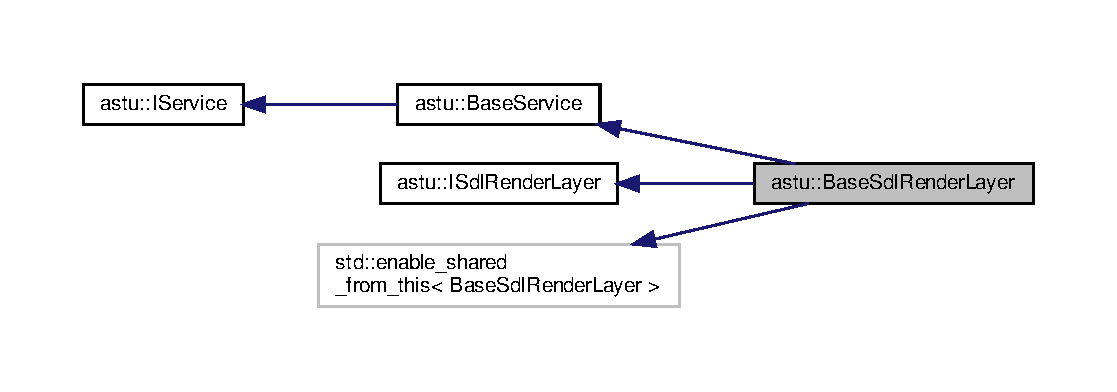
\includegraphics[width=350pt]{classastu_1_1BaseSdlRenderLayer__inherit__graph}
\end{center}
\end{figure}


Collaboration diagram for astu\+:\+:Base\+Sdl\+Render\+Layer\+:\nopagebreak
\begin{figure}[H]
\begin{center}
\leavevmode
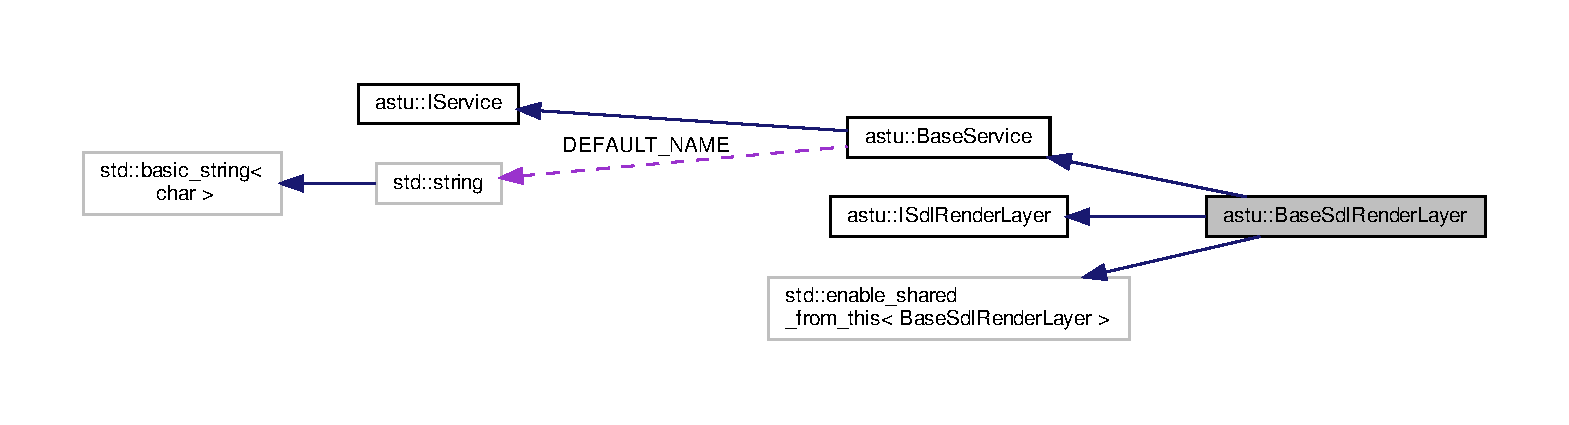
\includegraphics[width=350pt]{classastu_1_1BaseSdlRenderLayer__coll__graph}
\end{center}
\end{figure}
\subsection*{Public Member Functions}
\begin{DoxyCompactItemize}
\item 
\hyperlink{classastu_1_1BaseSdlRenderLayer_a9fc94044d6b75261798b1a1ead9e561d}{Base\+Sdl\+Render\+Layer} (int render\+Priority, const std\+::string \&name=\hyperlink{classastu_1_1BaseService_a9483b26ad631bd14646ef2d2170cd828}{Base\+Service\+::\+D\+E\+F\+A\+U\+L\+T\+\_\+\+N\+A\+ME})
\item 
virtual \hyperlink{classastu_1_1BaseSdlRenderLayer_a062e0d1188290dea9e8329265c114764}{$\sim$\+Base\+Sdl\+Render\+Layer} ()
\item 
virtual void \hyperlink{classastu_1_1BaseSdlRenderLayer_a0f4fbd9bbd5613589a8f1ce39d8b6340}{Startup} () override
\item 
virtual void \hyperlink{classastu_1_1BaseSdlRenderLayer_a786ae49f41873d498ae0d22a0f3a5349}{Shutdown} () override
\item 
virtual int \hyperlink{classastu_1_1BaseSdlRenderLayer_a612a7ecc518ea150bbed605a6aa19602}{Get\+Render\+Priority} () const final override
\item 
virtual void \hyperlink{classastu_1_1BaseSdlRenderLayer_a5b9f77db50819d6b29e0e8361d7fd91e}{On\+Resize} (int width, int height) override
\item 
int \hyperlink{classastu_1_1BaseSdlRenderLayer_a535b982190208e361f6b2c3cd717cb97}{Get\+Target\+Width} () const
\item 
int \hyperlink{classastu_1_1BaseSdlRenderLayer_a6e897555380c2ba39af2d6a10c79283f}{Get\+Target\+Height} () const
\end{DoxyCompactItemize}
\subsection*{Additional Inherited Members}


\subsection{Detailed Description}
Base class for services which implement the \hyperlink{classastu_1_1ISdlRenderLayer}{I\+Sdl\+Render\+Layer} interface. 

\subsection{Constructor \& Destructor Documentation}
\mbox{\Hypertarget{classastu_1_1BaseSdlRenderLayer_a9fc94044d6b75261798b1a1ead9e561d}\label{classastu_1_1BaseSdlRenderLayer_a9fc94044d6b75261798b1a1ead9e561d}} 
\index{astu\+::\+Base\+Sdl\+Render\+Layer@{astu\+::\+Base\+Sdl\+Render\+Layer}!Base\+Sdl\+Render\+Layer@{Base\+Sdl\+Render\+Layer}}
\index{Base\+Sdl\+Render\+Layer@{Base\+Sdl\+Render\+Layer}!astu\+::\+Base\+Sdl\+Render\+Layer@{astu\+::\+Base\+Sdl\+Render\+Layer}}
\subsubsection{\texorpdfstring{Base\+Sdl\+Render\+Layer()}{BaseSdlRenderLayer()}}
{\footnotesize\ttfamily astu\+::\+Base\+Sdl\+Render\+Layer\+::\+Base\+Sdl\+Render\+Layer (\begin{DoxyParamCaption}\item[{int}]{render\+Priority,  }\item[{const std\+::string \&}]{name = {\ttfamily \hyperlink{classastu_1_1BaseService_a9483b26ad631bd14646ef2d2170cd828}{Base\+Service\+::\+D\+E\+F\+A\+U\+L\+T\+\_\+\+N\+A\+ME}} }\end{DoxyParamCaption})}

Constructor.


\begin{DoxyParams}{Parameters}
{\em render\+Priority} & the render priority of this layer \\
\hline
{\em name} & the name of this service \\
\hline
\end{DoxyParams}
\mbox{\Hypertarget{classastu_1_1BaseSdlRenderLayer_a062e0d1188290dea9e8329265c114764}\label{classastu_1_1BaseSdlRenderLayer_a062e0d1188290dea9e8329265c114764}} 
\index{astu\+::\+Base\+Sdl\+Render\+Layer@{astu\+::\+Base\+Sdl\+Render\+Layer}!````~Base\+Sdl\+Render\+Layer@{$\sim$\+Base\+Sdl\+Render\+Layer}}
\index{````~Base\+Sdl\+Render\+Layer@{$\sim$\+Base\+Sdl\+Render\+Layer}!astu\+::\+Base\+Sdl\+Render\+Layer@{astu\+::\+Base\+Sdl\+Render\+Layer}}
\subsubsection{\texorpdfstring{$\sim$\+Base\+Sdl\+Render\+Layer()}{~BaseSdlRenderLayer()}}
{\footnotesize\ttfamily virtual astu\+::\+Base\+Sdl\+Render\+Layer\+::$\sim$\+Base\+Sdl\+Render\+Layer (\begin{DoxyParamCaption}{ }\end{DoxyParamCaption})\hspace{0.3cm}{\ttfamily [inline]}, {\ttfamily [virtual]}}

Virtual destructor. 

\subsection{Member Function Documentation}
\mbox{\Hypertarget{classastu_1_1BaseSdlRenderLayer_a612a7ecc518ea150bbed605a6aa19602}\label{classastu_1_1BaseSdlRenderLayer_a612a7ecc518ea150bbed605a6aa19602}} 
\index{astu\+::\+Base\+Sdl\+Render\+Layer@{astu\+::\+Base\+Sdl\+Render\+Layer}!Get\+Render\+Priority@{Get\+Render\+Priority}}
\index{Get\+Render\+Priority@{Get\+Render\+Priority}!astu\+::\+Base\+Sdl\+Render\+Layer@{astu\+::\+Base\+Sdl\+Render\+Layer}}
\subsubsection{\texorpdfstring{Get\+Render\+Priority()}{GetRenderPriority()}}
{\footnotesize\ttfamily virtual int astu\+::\+Base\+Sdl\+Render\+Layer\+::\+Get\+Render\+Priority (\begin{DoxyParamCaption}{ }\end{DoxyParamCaption}) const\hspace{0.3cm}{\ttfamily [final]}, {\ttfamily [override]}, {\ttfamily [virtual]}}

Returns the render priority. Lower priorities get rendered before higher priorities.

\begin{DoxyReturn}{Returns}
the render priority 
\end{DoxyReturn}


Implements \hyperlink{classastu_1_1ISdlRenderLayer_a623b411a1afa967bdaa879f5075eec43}{astu\+::\+I\+Sdl\+Render\+Layer}.

\mbox{\Hypertarget{classastu_1_1BaseSdlRenderLayer_a6e897555380c2ba39af2d6a10c79283f}\label{classastu_1_1BaseSdlRenderLayer_a6e897555380c2ba39af2d6a10c79283f}} 
\index{astu\+::\+Base\+Sdl\+Render\+Layer@{astu\+::\+Base\+Sdl\+Render\+Layer}!Get\+Target\+Height@{Get\+Target\+Height}}
\index{Get\+Target\+Height@{Get\+Target\+Height}!astu\+::\+Base\+Sdl\+Render\+Layer@{astu\+::\+Base\+Sdl\+Render\+Layer}}
\subsubsection{\texorpdfstring{Get\+Target\+Height()}{GetTargetHeight()}}
{\footnotesize\ttfamily int astu\+::\+Base\+Sdl\+Render\+Layer\+::\+Get\+Target\+Height (\begin{DoxyParamCaption}{ }\end{DoxyParamCaption}) const\hspace{0.3cm}{\ttfamily [inline]}}

Returns the height of the render taret.

\begin{DoxyReturn}{Returns}
the height in pixels 
\end{DoxyReturn}
\mbox{\Hypertarget{classastu_1_1BaseSdlRenderLayer_a535b982190208e361f6b2c3cd717cb97}\label{classastu_1_1BaseSdlRenderLayer_a535b982190208e361f6b2c3cd717cb97}} 
\index{astu\+::\+Base\+Sdl\+Render\+Layer@{astu\+::\+Base\+Sdl\+Render\+Layer}!Get\+Target\+Width@{Get\+Target\+Width}}
\index{Get\+Target\+Width@{Get\+Target\+Width}!astu\+::\+Base\+Sdl\+Render\+Layer@{astu\+::\+Base\+Sdl\+Render\+Layer}}
\subsubsection{\texorpdfstring{Get\+Target\+Width()}{GetTargetWidth()}}
{\footnotesize\ttfamily int astu\+::\+Base\+Sdl\+Render\+Layer\+::\+Get\+Target\+Width (\begin{DoxyParamCaption}{ }\end{DoxyParamCaption}) const\hspace{0.3cm}{\ttfamily [inline]}}

Returns the width of the render taret.

\begin{DoxyReturn}{Returns}
the width in pixels 
\end{DoxyReturn}
\mbox{\Hypertarget{classastu_1_1BaseSdlRenderLayer_a5b9f77db50819d6b29e0e8361d7fd91e}\label{classastu_1_1BaseSdlRenderLayer_a5b9f77db50819d6b29e0e8361d7fd91e}} 
\index{astu\+::\+Base\+Sdl\+Render\+Layer@{astu\+::\+Base\+Sdl\+Render\+Layer}!On\+Resize@{On\+Resize}}
\index{On\+Resize@{On\+Resize}!astu\+::\+Base\+Sdl\+Render\+Layer@{astu\+::\+Base\+Sdl\+Render\+Layer}}
\subsubsection{\texorpdfstring{On\+Resize()}{OnResize()}}
{\footnotesize\ttfamily virtual void astu\+::\+Base\+Sdl\+Render\+Layer\+::\+On\+Resize (\begin{DoxyParamCaption}\item[{int}]{width,  }\item[{int}]{height }\end{DoxyParamCaption})\hspace{0.3cm}{\ttfamily [override]}, {\ttfamily [virtual]}}

Called when the size of the render target has changed.

It is guaranteed that this method is called at least once before the first call of {\ttfamily On\+Render}.


\begin{DoxyParams}{Parameters}
{\em width} & the width of the render target in pixels \\
\hline
{\em height} & the height of the render target in pixels \\
\hline
\end{DoxyParams}


Implements \hyperlink{classastu_1_1ISdlRenderLayer_abcded808a2405e1e59413b5d1f981f13}{astu\+::\+I\+Sdl\+Render\+Layer}.

\mbox{\Hypertarget{classastu_1_1BaseSdlRenderLayer_a786ae49f41873d498ae0d22a0f3a5349}\label{classastu_1_1BaseSdlRenderLayer_a786ae49f41873d498ae0d22a0f3a5349}} 
\index{astu\+::\+Base\+Sdl\+Render\+Layer@{astu\+::\+Base\+Sdl\+Render\+Layer}!Shutdown@{Shutdown}}
\index{Shutdown@{Shutdown}!astu\+::\+Base\+Sdl\+Render\+Layer@{astu\+::\+Base\+Sdl\+Render\+Layer}}
\subsubsection{\texorpdfstring{Shutdown()}{Shutdown()}}
{\footnotesize\ttfamily virtual void astu\+::\+Base\+Sdl\+Render\+Layer\+::\+Shutdown (\begin{DoxyParamCaption}{ }\end{DoxyParamCaption})\hspace{0.3cm}{\ttfamily [override]}, {\ttfamily [virtual]}}

Stops this service.

In case this service is currently not running, calling this method has no effect. 

Reimplemented from \hyperlink{classastu_1_1BaseService_a7095888244052db294d58738c0d187fb}{astu\+::\+Base\+Service}.

\mbox{\Hypertarget{classastu_1_1BaseSdlRenderLayer_a0f4fbd9bbd5613589a8f1ce39d8b6340}\label{classastu_1_1BaseSdlRenderLayer_a0f4fbd9bbd5613589a8f1ce39d8b6340}} 
\index{astu\+::\+Base\+Sdl\+Render\+Layer@{astu\+::\+Base\+Sdl\+Render\+Layer}!Startup@{Startup}}
\index{Startup@{Startup}!astu\+::\+Base\+Sdl\+Render\+Layer@{astu\+::\+Base\+Sdl\+Render\+Layer}}
\subsubsection{\texorpdfstring{Startup()}{Startup()}}
{\footnotesize\ttfamily virtual void astu\+::\+Base\+Sdl\+Render\+Layer\+::\+Startup (\begin{DoxyParamCaption}{ }\end{DoxyParamCaption})\hspace{0.3cm}{\ttfamily [override]}, {\ttfamily [virtual]}}

Starts this service.


\begin{DoxyExceptions}{Exceptions}
{\em std\+::logic\+\_\+error} & in case this service is already running \\
\hline
\end{DoxyExceptions}


Reimplemented from \hyperlink{classastu_1_1BaseService_a59dade033dcb44dd32155c526a3a58e2}{astu\+::\+Base\+Service}.



The documentation for this class was generated from the following file\+:\begin{DoxyCompactItemize}
\item 
include/Sdl\+Render\+Service.\+h\end{DoxyCompactItemize}

\hypertarget{classastu_1_1BaseService}{}\section{astu\+:\+:Base\+Service Class Reference}
\label{classastu_1_1BaseService}\index{astu\+::\+Base\+Service@{astu\+::\+Base\+Service}}


{\ttfamily \#include $<$Service.\+h$>$}



Inheritance diagram for astu\+:\+:Base\+Service\+:\nopagebreak
\begin{figure}[H]
\begin{center}
\leavevmode
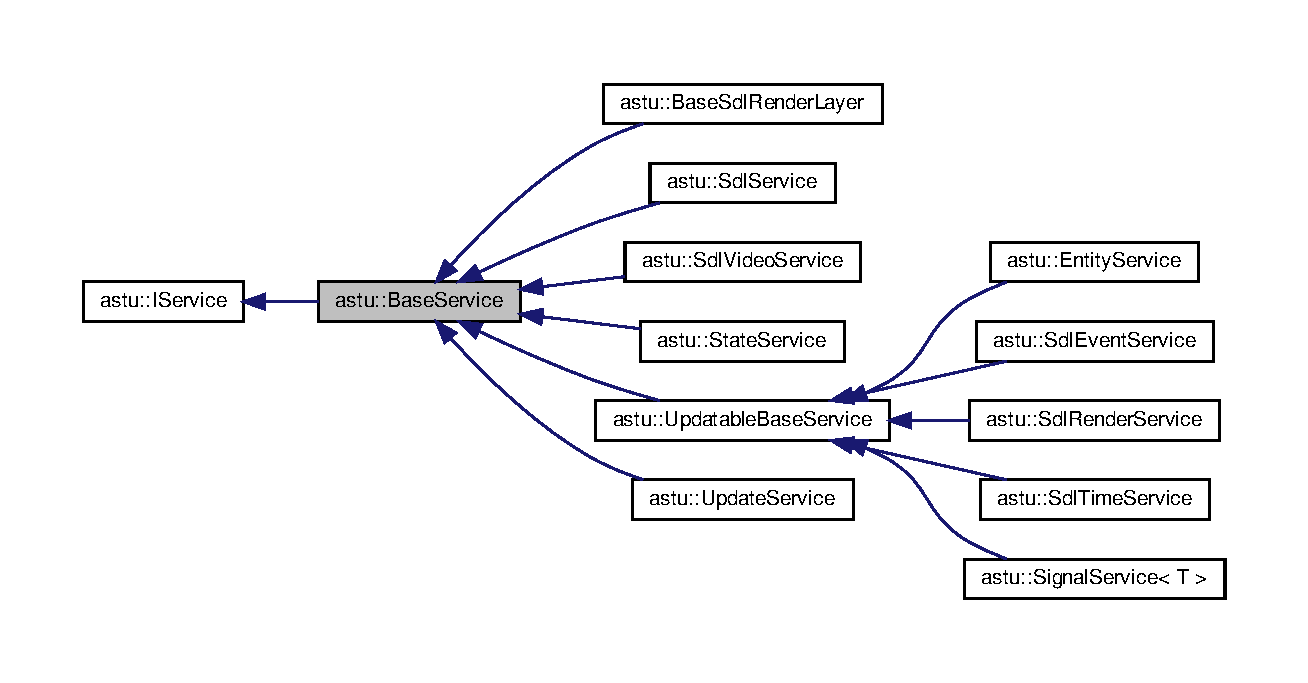
\includegraphics[width=350pt]{classastu_1_1BaseService__inherit__graph}
\end{center}
\end{figure}


Collaboration diagram for astu\+:\+:Base\+Service\+:\nopagebreak
\begin{figure}[H]
\begin{center}
\leavevmode
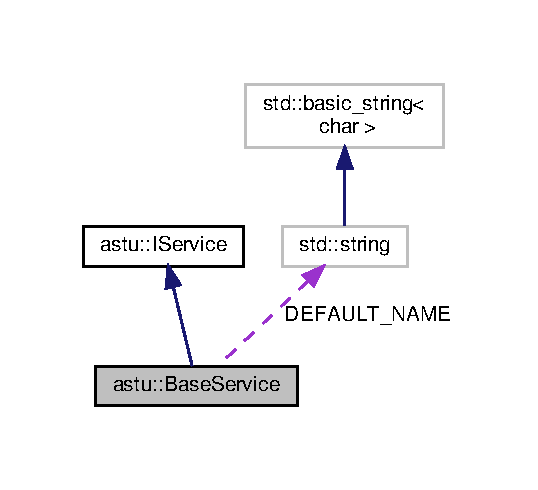
\includegraphics[width=258pt]{classastu_1_1BaseService__coll__graph}
\end{center}
\end{figure}
\subsection*{Public Member Functions}
\begin{DoxyCompactItemize}
\item 
\hyperlink{classastu_1_1BaseService_ab155c73d180c22dab7cf8aff1514b2b5}{Base\+Service} (const std\+::string \&name=\hyperlink{classastu_1_1BaseService_a9483b26ad631bd14646ef2d2170cd828}{D\+E\+F\+A\+U\+L\+T\+\_\+\+N\+A\+ME})
\item 
virtual const std\+::string \& \hyperlink{classastu_1_1BaseService_a42eb6e0d667215ef635682d2a12e1631}{Get\+Name} () const final override
\item 
virtual void \hyperlink{classastu_1_1BaseService_a59dade033dcb44dd32155c526a3a58e2}{Startup} () override
\item 
virtual void \hyperlink{classastu_1_1BaseService_a7095888244052db294d58738c0d187fb}{Shutdown} () override
\item 
virtual bool \hyperlink{classastu_1_1BaseService_af6f4641c045343d329a0fc1ecc6a9778}{Is\+Running} () const override
\end{DoxyCompactItemize}
\subsection*{Static Public Attributes}
\begin{DoxyCompactItemize}
\item 
static const std\+::string \& \hyperlink{classastu_1_1BaseService_a9483b26ad631bd14646ef2d2170cd828}{D\+E\+F\+A\+U\+L\+T\+\_\+\+N\+A\+ME}
\end{DoxyCompactItemize}
\subsection*{Protected Member Functions}
\begin{DoxyCompactItemize}
\item 
virtual void \hyperlink{classastu_1_1BaseService_ac8710cd2d6dcc990db65e7c8ccfbc5ff}{On\+Startup} ()
\item 
virtual void \hyperlink{classastu_1_1BaseService_aeb5003f7c5efe5412725ac4c66942d03}{On\+Shutdown} ()
\item 
\hyperlink{classastu_1_1ServiceManager}{Service\+Manager} \& \hyperlink{classastu_1_1BaseService_a646b6c83a9ebd26fe4e7796b5afde612}{Get\+SM} ()
\end{DoxyCompactItemize}


\subsection{Detailed Description}
Implmenents basic functionality of a service.

This base class can be used to create services with basic functionlality e.\+g, having a name and keeping track if its currently running or not. 

\subsection{Constructor \& Destructor Documentation}
\mbox{\Hypertarget{classastu_1_1BaseService_ab155c73d180c22dab7cf8aff1514b2b5}\label{classastu_1_1BaseService_ab155c73d180c22dab7cf8aff1514b2b5}} 
\index{astu\+::\+Base\+Service@{astu\+::\+Base\+Service}!Base\+Service@{Base\+Service}}
\index{Base\+Service@{Base\+Service}!astu\+::\+Base\+Service@{astu\+::\+Base\+Service}}
\subsubsection{\texorpdfstring{Base\+Service()}{BaseService()}}
{\footnotesize\ttfamily astu\+::\+Base\+Service\+::\+Base\+Service (\begin{DoxyParamCaption}\item[{const std\+::string \&}]{name = {\ttfamily \hyperlink{classastu_1_1BaseService_a9483b26ad631bd14646ef2d2170cd828}{D\+E\+F\+A\+U\+L\+T\+\_\+\+N\+A\+ME}} }\end{DoxyParamCaption})}

Constructor. 

\subsection{Member Function Documentation}
\mbox{\Hypertarget{classastu_1_1BaseService_a42eb6e0d667215ef635682d2a12e1631}\label{classastu_1_1BaseService_a42eb6e0d667215ef635682d2a12e1631}} 
\index{astu\+::\+Base\+Service@{astu\+::\+Base\+Service}!Get\+Name@{Get\+Name}}
\index{Get\+Name@{Get\+Name}!astu\+::\+Base\+Service@{astu\+::\+Base\+Service}}
\subsubsection{\texorpdfstring{Get\+Name()}{GetName()}}
{\footnotesize\ttfamily virtual const std\+::string\& astu\+::\+Base\+Service\+::\+Get\+Name (\begin{DoxyParamCaption}{ }\end{DoxyParamCaption}) const\hspace{0.3cm}{\ttfamily [final]}, {\ttfamily [override]}, {\ttfamily [virtual]}}

Returns the name of this service.

\begin{DoxyReturn}{Returns}
this service\textquotesingle{}s name 
\end{DoxyReturn}


Implements \hyperlink{classastu_1_1IService_a7bfb508c07816c701ceaa72928213380}{astu\+::\+I\+Service}.

\mbox{\Hypertarget{classastu_1_1BaseService_a646b6c83a9ebd26fe4e7796b5afde612}\label{classastu_1_1BaseService_a646b6c83a9ebd26fe4e7796b5afde612}} 
\index{astu\+::\+Base\+Service@{astu\+::\+Base\+Service}!Get\+SM@{Get\+SM}}
\index{Get\+SM@{Get\+SM}!astu\+::\+Base\+Service@{astu\+::\+Base\+Service}}
\subsubsection{\texorpdfstring{Get\+S\+M()}{GetSM()}}
{\footnotesize\ttfamily \hyperlink{classastu_1_1ServiceManager}{Service\+Manager}\& astu\+::\+Base\+Service\+::\+Get\+SM (\begin{DoxyParamCaption}{ }\end{DoxyParamCaption})\hspace{0.3cm}{\ttfamily [protected]}}

Returns the service manager.

This method is right now just a convenience method to get access tot the service manager. However future version of this service module might make use of multiple different service manages instead of using a singleton. In this case this method becomes a requirement.

\begin{DoxyReturn}{Returns}
the service manager 
\end{DoxyReturn}
\mbox{\Hypertarget{classastu_1_1BaseService_af6f4641c045343d329a0fc1ecc6a9778}\label{classastu_1_1BaseService_af6f4641c045343d329a0fc1ecc6a9778}} 
\index{astu\+::\+Base\+Service@{astu\+::\+Base\+Service}!Is\+Running@{Is\+Running}}
\index{Is\+Running@{Is\+Running}!astu\+::\+Base\+Service@{astu\+::\+Base\+Service}}
\subsubsection{\texorpdfstring{Is\+Running()}{IsRunning()}}
{\footnotesize\ttfamily virtual bool astu\+::\+Base\+Service\+::\+Is\+Running (\begin{DoxyParamCaption}{ }\end{DoxyParamCaption}) const\hspace{0.3cm}{\ttfamily [override]}, {\ttfamily [virtual]}}

Returns {\ttfamily true} if this service is running.

\begin{DoxyReturn}{Returns}
{\ttfamily true} if this service is running 
\end{DoxyReturn}


Implements \hyperlink{classastu_1_1IService_ab69225f6a613c8829c45d23158fba775}{astu\+::\+I\+Service}.

\mbox{\Hypertarget{classastu_1_1BaseService_aeb5003f7c5efe5412725ac4c66942d03}\label{classastu_1_1BaseService_aeb5003f7c5efe5412725ac4c66942d03}} 
\index{astu\+::\+Base\+Service@{astu\+::\+Base\+Service}!On\+Shutdown@{On\+Shutdown}}
\index{On\+Shutdown@{On\+Shutdown}!astu\+::\+Base\+Service@{astu\+::\+Base\+Service}}
\subsubsection{\texorpdfstring{On\+Shutdown()}{OnShutdown()}}
{\footnotesize\ttfamily virtual void astu\+::\+Base\+Service\+::\+On\+Shutdown (\begin{DoxyParamCaption}{ }\end{DoxyParamCaption})\hspace{0.3cm}{\ttfamily [inline]}, {\ttfamily [protected]}, {\ttfamily [virtual]}}

Called by this base class on shutdown.

Derived classes should override this method rather than {\ttfamily \hyperlink{classastu_1_1BaseService_a7095888244052db294d58738c0d187fb}{Shutdown()}}. The {\ttfamily \hyperlink{classastu_1_1BaseService_a7095888244052db294d58738c0d187fb}{Shutdown()}} method is maintaining the running-\/state of this service. 

Reimplemented in \hyperlink{classastu_1_1EntityService_ac998c4d02a90460a129c8f2e0586d728}{astu\+::\+Entity\+Service}, \hyperlink{classastu_1_1SdlRenderService_a4f21478ca10de11d260792c3ccd79eef}{astu\+::\+Sdl\+Render\+Service}, \hyperlink{classastu_1_1StateService_ad8fa5b6d52bd795ebba450f119540d87}{astu\+::\+State\+Service}, \hyperlink{classastu_1_1SdlVideoService_a6d6085e9ff213c5d41546d604ff53e92}{astu\+::\+Sdl\+Video\+Service}, \hyperlink{classastu_1_1SdlEventService_a0163bd191605b5068d93cd6c8f26da0c}{astu\+::\+Sdl\+Event\+Service}, \hyperlink{classastu_1_1SdlTimeService_a6a1b864beed186413933dd8b97a393a2}{astu\+::\+Sdl\+Time\+Service}, and \hyperlink{classastu_1_1SdlService_a20d53237efd1c717d773a8ff121b093b}{astu\+::\+Sdl\+Service}.

\mbox{\Hypertarget{classastu_1_1BaseService_ac8710cd2d6dcc990db65e7c8ccfbc5ff}\label{classastu_1_1BaseService_ac8710cd2d6dcc990db65e7c8ccfbc5ff}} 
\index{astu\+::\+Base\+Service@{astu\+::\+Base\+Service}!On\+Startup@{On\+Startup}}
\index{On\+Startup@{On\+Startup}!astu\+::\+Base\+Service@{astu\+::\+Base\+Service}}
\subsubsection{\texorpdfstring{On\+Startup()}{OnStartup()}}
{\footnotesize\ttfamily virtual void astu\+::\+Base\+Service\+::\+On\+Startup (\begin{DoxyParamCaption}{ }\end{DoxyParamCaption})\hspace{0.3cm}{\ttfamily [inline]}, {\ttfamily [protected]}, {\ttfamily [virtual]}}

Called by this base class on startup.

Derived classes should override this method rather than {\ttfamily \hyperlink{classastu_1_1BaseService_a59dade033dcb44dd32155c526a3a58e2}{Startup()}}. The {\ttfamily \hyperlink{classastu_1_1BaseService_a59dade033dcb44dd32155c526a3a58e2}{Startup()}} method is maintaining the running-\/state of this service. 

Reimplemented in \hyperlink{classastu_1_1EntityService_a293ff7c8b84837b08cdabe98ed8a23ea}{astu\+::\+Entity\+Service}, \hyperlink{classastu_1_1SdlRenderService_a38abd541e8075e5e4eb702ca99c9b0a5}{astu\+::\+Sdl\+Render\+Service}, \hyperlink{classastu_1_1StateService_a06419feca958b72db99dde6eda301f86}{astu\+::\+State\+Service}, \hyperlink{classastu_1_1SdlVideoService_add229ac2af59a4aea090e4de4c67e530}{astu\+::\+Sdl\+Video\+Service}, \hyperlink{classastu_1_1SdlEventService_a71805a124600a23e48158daa5dc57fff}{astu\+::\+Sdl\+Event\+Service}, \hyperlink{classastu_1_1SdlTimeService_ac11551691bb14289020028a2a162c7d6}{astu\+::\+Sdl\+Time\+Service}, and \hyperlink{classastu_1_1SdlService_a2fcb46537de794ab6e4f5e043b26ff60}{astu\+::\+Sdl\+Service}.

\mbox{\Hypertarget{classastu_1_1BaseService_a7095888244052db294d58738c0d187fb}\label{classastu_1_1BaseService_a7095888244052db294d58738c0d187fb}} 
\index{astu\+::\+Base\+Service@{astu\+::\+Base\+Service}!Shutdown@{Shutdown}}
\index{Shutdown@{Shutdown}!astu\+::\+Base\+Service@{astu\+::\+Base\+Service}}
\subsubsection{\texorpdfstring{Shutdown()}{Shutdown()}}
{\footnotesize\ttfamily virtual void astu\+::\+Base\+Service\+::\+Shutdown (\begin{DoxyParamCaption}{ }\end{DoxyParamCaption})\hspace{0.3cm}{\ttfamily [override]}, {\ttfamily [virtual]}}

Stops this service.

In case this service is currently not running, calling this method has no effect. 

Implements \hyperlink{classastu_1_1IService_a67643385e7cc17c31e0b3b49672b5856}{astu\+::\+I\+Service}.



Reimplemented in \hyperlink{classastu_1_1BaseSdlRenderLayer_a786ae49f41873d498ae0d22a0f3a5349}{astu\+::\+Base\+Sdl\+Render\+Layer}, and \hyperlink{classastu_1_1UpdatableBaseService_a7ad7e0201007878b6014361dd5ba82f9}{astu\+::\+Updatable\+Base\+Service}.

\mbox{\Hypertarget{classastu_1_1BaseService_a59dade033dcb44dd32155c526a3a58e2}\label{classastu_1_1BaseService_a59dade033dcb44dd32155c526a3a58e2}} 
\index{astu\+::\+Base\+Service@{astu\+::\+Base\+Service}!Startup@{Startup}}
\index{Startup@{Startup}!astu\+::\+Base\+Service@{astu\+::\+Base\+Service}}
\subsubsection{\texorpdfstring{Startup()}{Startup()}}
{\footnotesize\ttfamily virtual void astu\+::\+Base\+Service\+::\+Startup (\begin{DoxyParamCaption}{ }\end{DoxyParamCaption})\hspace{0.3cm}{\ttfamily [override]}, {\ttfamily [virtual]}}

Starts this service.


\begin{DoxyExceptions}{Exceptions}
{\em std\+::logic\+\_\+error} & in case this service is already running \\
\hline
\end{DoxyExceptions}


Implements \hyperlink{classastu_1_1IService_a7a09e485d116659f174aca9a8494fa55}{astu\+::\+I\+Service}.



Reimplemented in \hyperlink{classastu_1_1BaseSdlRenderLayer_a0f4fbd9bbd5613589a8f1ce39d8b6340}{astu\+::\+Base\+Sdl\+Render\+Layer}, and \hyperlink{classastu_1_1UpdatableBaseService_a47e3725f717cee3cd8983f485b2a0243}{astu\+::\+Updatable\+Base\+Service}.



\subsection{Member Data Documentation}
\mbox{\Hypertarget{classastu_1_1BaseService_a9483b26ad631bd14646ef2d2170cd828}\label{classastu_1_1BaseService_a9483b26ad631bd14646ef2d2170cd828}} 
\index{astu\+::\+Base\+Service@{astu\+::\+Base\+Service}!D\+E\+F\+A\+U\+L\+T\+\_\+\+N\+A\+ME@{D\+E\+F\+A\+U\+L\+T\+\_\+\+N\+A\+ME}}
\index{D\+E\+F\+A\+U\+L\+T\+\_\+\+N\+A\+ME@{D\+E\+F\+A\+U\+L\+T\+\_\+\+N\+A\+ME}!astu\+::\+Base\+Service@{astu\+::\+Base\+Service}}
\subsubsection{\texorpdfstring{D\+E\+F\+A\+U\+L\+T\+\_\+\+N\+A\+ME}{DEFAULT\_NAME}}
{\footnotesize\ttfamily const std\+::string\& astu\+::\+Base\+Service\+::\+D\+E\+F\+A\+U\+L\+T\+\_\+\+N\+A\+ME\hspace{0.3cm}{\ttfamily [static]}}

Default name for services. 

The documentation for this class was generated from the following file\+:\begin{DoxyCompactItemize}
\item 
include/Service.\+h\end{DoxyCompactItemize}

\hypertarget{classastu_1_1Color}{}\section{astu\+:\+:Color$<$ T $>$ Class Template Reference}
\label{classastu_1_1Color}\index{astu\+::\+Color$<$ T $>$@{astu\+::\+Color$<$ T $>$}}


{\ttfamily \#include $<$Color.\+h$>$}



Collaboration diagram for astu\+:\+:Color$<$ T $>$\+:\nopagebreak
\begin{figure}[H]
\begin{center}
\leavevmode
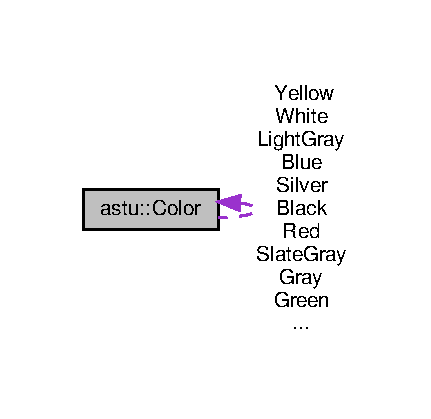
\includegraphics[width=169pt]{classastu_1_1Color__coll__graph}
\end{center}
\end{figure}
\subsection*{Public Member Functions}
\begin{DoxyCompactItemize}
\item 
\hyperlink{classastu_1_1Color_abb0e2cdad572357375d5b2465ea847b9}{Color} (T red=0, T green=0, T blue=0, T alpha=1)
\item 
\hyperlink{classastu_1_1Color_a1ce283cfd9542b85da611fc50a4a9e54}{Color} (int rgb)
\item 
\hyperlink{classastu_1_1Color}{Color}$<$ T $>$ \& \hyperlink{classastu_1_1Color_a0fcfa896c3a32ae0af1aeec3f4d866fe}{Set\+Alpha} (T \hyperlink{classastu_1_1Color_ad62b3af3464dea4bf99432bfb6e9d796}{a})
\item 
void \hyperlink{classastu_1_1Color_ad5aaf54919fed257c37b6b5747bd01c8}{Set} (T red, T green, T blue, T alpha=1)
\item 
int \hyperlink{classastu_1_1Color_a376a9d08b37e917a7040d58aab009bf5}{To\+Rgba} () const
\item 
T \hyperlink{classastu_1_1Color_a4802f8f0d0fcf65ba6853ac17c52b811}{Distance\+Without\+Alpha} (const \hyperlink{classastu_1_1Color}{Color}$<$ T $>$ \&o) const
\item 
T \hyperlink{classastu_1_1Color_a35549a6d06ab1fbc8a232508e3041f9d}{Distance\+Squared\+Without\+Alpha} (const \hyperlink{classastu_1_1Color}{Color}$<$ T $>$ \&o) const
\item 
T \hyperlink{classastu_1_1Color_aa61d12089e02ec0ce02ab877b21c6bcc}{Distance} (const \hyperlink{classastu_1_1Color}{Color}$<$ T $>$ \&o) const
\item 
T \hyperlink{classastu_1_1Color_a9b396fa9b0d3612ec9eb372b52de1eac}{Distance\+Squared} (const \hyperlink{classastu_1_1Color}{Color}$<$ T $>$ \&o) const
\item 
\hyperlink{classastu_1_1Color}{Color}$<$ T $>$ \& \hyperlink{classastu_1_1Color_a662946707019ddc5d79612da685be5f8}{Multiply\+Without\+Alpha} (T s) noexcept
\item 
int \hyperlink{classastu_1_1Color_aa7c679fe7a6c4b11ea163bc1d64fd73b}{Get\+A\+R\+GB} () const
\item 
int \hyperlink{classastu_1_1Color_a11cf3e00ee1662cc67aae0fa5767df39}{Get\+A\+B\+GR} () const
\item 
\hyperlink{classastu_1_1Color}{Color}$<$ T $>$ \& \hyperlink{classastu_1_1Color_a60780325071ef6c95b113f9f5f9905b4}{Saturate} () noexcept
\item 
\hyperlink{classastu_1_1Color}{Color}$<$ T $>$ \& \hyperlink{classastu_1_1Color_a33b9d43c6d2306ccd7e3071e0e52eb25}{Blend} (const \hyperlink{classastu_1_1Color}{Color}$<$ T $>$ \&o)
\item 
\hyperlink{classastu_1_1Color}{Color}$<$ T $>$ \hyperlink{classastu_1_1Color_acc63e1fac50adf874fa5b33516186e7f}{Lerp} (const \hyperlink{classastu_1_1Color}{Color}$<$ T $>$ \&o, T t) const
\item 
\hyperlink{classastu_1_1Color}{Color}$<$ T $>$ \hyperlink{classastu_1_1Color_a7f1c0093d51c4036f7ab5755d571d6e7}{operator+} (const \hyperlink{classastu_1_1Color}{Color}$<$ T $>$ \&rhs) const
\item 
\hyperlink{classastu_1_1Color}{Color}$<$ T $>$ \& \hyperlink{classastu_1_1Color_ab4cafbc5cbd4aa28a8feb428107d3985}{operator+=} (const \hyperlink{classastu_1_1Color}{Color}$<$ T $>$ \&rhs)
\item 
\hyperlink{classastu_1_1Color}{Color}$<$ T $>$ \hyperlink{classastu_1_1Color_a2d512332791d4187ecde51771648cb9c}{operator-\/} (const \hyperlink{classastu_1_1Color}{Color}$<$ T $>$ \&rhs) const
\item 
\hyperlink{classastu_1_1Color}{Color}$<$ T $>$ \& \hyperlink{classastu_1_1Color_add622a013366f3f07eee482493c2c158}{operator-\/=} (const \hyperlink{classastu_1_1Color}{Color}$<$ T $>$ \&rhs)
\item 
\hyperlink{classastu_1_1Color}{Color}$<$ T $>$ \hyperlink{classastu_1_1Color_aa1fc446d899409058a6e510775ae009d}{operator$\ast$} (T s) const
\item 
\hyperlink{classastu_1_1Color}{Color}$<$ T $>$ \& \hyperlink{classastu_1_1Color_ab097615260001619304f4d128b484359}{operator$\ast$=} (T s)
\item 
\hyperlink{classastu_1_1Color}{Color}$<$ T $>$ \hyperlink{classastu_1_1Color_af4b143f6c4c3b15412293a25f05320b2}{operator/} (T s) const
\item 
\hyperlink{classastu_1_1Color}{Color}$<$ T $>$ \& \hyperlink{classastu_1_1Color_a8411cf3d645429dbcdc609a8db010c68}{operator/=} (T s)
\item 
bool \hyperlink{classastu_1_1Color_a3cfd5f7a4157b012c4ca1df92289e525}{operator==} (const \hyperlink{classastu_1_1Color}{Color}$<$ T $>$ \&o) const
\item 
bool \hyperlink{classastu_1_1Color_a03214300c75b0737cd91679f758112c5}{operator!=} (const \hyperlink{classastu_1_1Color}{Color}$<$ T $>$ \&o) const
\item 
bool \hyperlink{classastu_1_1Color_a3ff28065c93ca64d4806186118eef206}{operator$<$} (const \hyperlink{classastu_1_1Color}{Color}$<$ T $>$ \&rhs) const
\end{DoxyCompactItemize}
\subsection*{Static Public Member Functions}
\begin{DoxyCompactItemize}
\item 
static \hyperlink{classastu_1_1Color}{Color}$<$ T $>$ \hyperlink{classastu_1_1Color_a02abdb3a0d65626cb6bae8cbad7d6dfd}{Create\+From\+Rgb} (int red, int green, int blue, int alpha=255)
\end{DoxyCompactItemize}
\subsection*{Public Attributes}
\begin{DoxyCompactItemize}
\item 
T \hyperlink{classastu_1_1Color_aa670f74822e1db4513844dca52b1eb6a}{r}
\item 
T \hyperlink{classastu_1_1Color_a3134881dda38a8f123387faeff309dff}{g}
\item 
T \hyperlink{classastu_1_1Color_a56d075e69ca5e4cea336f3977b04dee2}{b}
\item 
T \hyperlink{classastu_1_1Color_ad62b3af3464dea4bf99432bfb6e9d796}{a}
\end{DoxyCompactItemize}


\subsection{Detailed Description}
\subsubsection*{template$<$typename T$>$\newline
class astu\+::\+Color$<$ T $>$}

Represents a color value in R\+GB color space.

A color is described using four color channels\+: red, green, blue and alpha. The alpha channel represents transparency. The color channels are represents as floating-\/point values which normally lie within the interval \mbox{[}0, 1\mbox{]}. 

\subsection{Constructor \& Destructor Documentation}
\mbox{\Hypertarget{classastu_1_1Color_abb0e2cdad572357375d5b2465ea847b9}\label{classastu_1_1Color_abb0e2cdad572357375d5b2465ea847b9}} 
\index{astu\+::\+Color@{astu\+::\+Color}!Color@{Color}}
\index{Color@{Color}!astu\+::\+Color@{astu\+::\+Color}}
\subsubsection{\texorpdfstring{Color()}{Color()}\hspace{0.1cm}{\footnotesize\ttfamily [1/2]}}
{\footnotesize\ttfamily template$<$typename T$>$ \\
\hyperlink{classastu_1_1Color}{astu\+::\+Color}$<$ T $>$\+::\hyperlink{classastu_1_1Color}{Color} (\begin{DoxyParamCaption}\item[{T}]{red = {\ttfamily 0},  }\item[{T}]{green = {\ttfamily 0},  }\item[{T}]{blue = {\ttfamily 0},  }\item[{T}]{alpha = {\ttfamily 1} }\end{DoxyParamCaption})\hspace{0.3cm}{\ttfamily [inline]}}

Constructor.


\begin{DoxyParams}{Parameters}
{\em red} & the red color component \\
\hline
{\em green} & the green color component \\
\hline
{\em blue} & the blue color component \\
\hline
{\em alpha} & the alpha color component \\
\hline
\end{DoxyParams}
\mbox{\Hypertarget{classastu_1_1Color_a1ce283cfd9542b85da611fc50a4a9e54}\label{classastu_1_1Color_a1ce283cfd9542b85da611fc50a4a9e54}} 
\index{astu\+::\+Color@{astu\+::\+Color}!Color@{Color}}
\index{Color@{Color}!astu\+::\+Color@{astu\+::\+Color}}
\subsubsection{\texorpdfstring{Color()}{Color()}\hspace{0.1cm}{\footnotesize\ttfamily [2/2]}}
{\footnotesize\ttfamily template$<$typename T$>$ \\
\hyperlink{classastu_1_1Color}{astu\+::\+Color}$<$ T $>$\+::\hyperlink{classastu_1_1Color}{Color} (\begin{DoxyParamCaption}\item[{int}]{rgb }\end{DoxyParamCaption})\hspace{0.3cm}{\ttfamily [inline]}}

Constructor.

This constructor can be used to create colors using the usual hex-\/triplet notation which is a six-\/digit, three-\/byte hexadecimal number used int H\+T\+ML, C\+SS, S\+VG etc.

{\bfseries Example}


\begin{DoxyCode}
\hyperlink{classastu_1_1Color_abb0e2cdad572357375d5b2465ea847b9}{Color} mediumAquamarine(0x66cdaa);
\end{DoxyCode}


The enum \hyperlink{classastu_1_1WebColors}{Web\+Colors} defines integer constants according to the color names defined by the W3C standards. These constants can be used to initialize colors using this constructor.


\begin{DoxyCode}
\hyperlink{classastu_1_1Color_abb0e2cdad572357375d5b2465ea847b9}{Color} redColor(\hyperlink{classastu_1_1WebColors_ac75482e858498b1b3fa521ba93fcda98a56bb31647b5e647e11d2941f54a30781}{WebColors::Red});
\hyperlink{classastu_1_1Color_abb0e2cdad572357375d5b2465ea847b9}{Color} PurpleColor(\hyperlink{classastu_1_1WebColors_ac75482e858498b1b3fa521ba93fcda98a3d63297abeb7cf60c2ddae0a1ee3e658}{WebColors::Purple});
\end{DoxyCode}


This constructor also functions as automatic conversion constructor which allows C++ to automatically convert integers to objects of class \hyperlink{classastu_1_1Color}{Color}. This makes it particularly easy to use the Web\+Color constants to initialize colors\+:


\begin{DoxyCode}
\hyperlink{classastu_1_1Color_abb0e2cdad572357375d5b2465ea847b9}{Color} redColor = \hyperlink{classastu_1_1WebColors_ac75482e858498b1b3fa521ba93fcda98a56bb31647b5e647e11d2941f54a30781}{WebColors::Red};
\end{DoxyCode}


or even as function arguments of type color


\begin{DoxyCode}
\textcolor{preprocessor}{#include <Color.h>}

\textcolor{keywordtype}{void} SomeFunction(\textcolor{keyword}{const} \hyperlink{classastu_1_1Color_abb0e2cdad572357375d5b2465ea847b9}{Color} & c) \{
 \textcolor{comment}{// Does something with c...}
\}

\textcolor{keywordtype}{int} main() \{
  SomeFunction(\hyperlink{classastu_1_1WebColors_ac75482e858498b1b3fa521ba93fcda98a93a4bd8dbcd8c09329c7d866c835571c}{WebColors::Aqua});

  \textcolor{keywordflow}{return} 0;
\}
\end{DoxyCode}



\begin{DoxyParams}{Parameters}
{\em rgb} & the rgb color components encoded within in an integer \\
\hline
\end{DoxyParams}


\subsection{Member Function Documentation}
\mbox{\Hypertarget{classastu_1_1Color_a33b9d43c6d2306ccd7e3071e0e52eb25}\label{classastu_1_1Color_a33b9d43c6d2306ccd7e3071e0e52eb25}} 
\index{astu\+::\+Color@{astu\+::\+Color}!Blend@{Blend}}
\index{Blend@{Blend}!astu\+::\+Color@{astu\+::\+Color}}
\subsubsection{\texorpdfstring{Blend()}{Blend()}}
{\footnotesize\ttfamily template$<$typename T$>$ \\
\hyperlink{classastu_1_1Color}{Color}$<$T$>$\& \hyperlink{classastu_1_1Color}{astu\+::\+Color}$<$ T $>$\+::Blend (\begin{DoxyParamCaption}\item[{const \hyperlink{classastu_1_1Color}{Color}$<$ T $>$ \&}]{o }\end{DoxyParamCaption})\hspace{0.3cm}{\ttfamily [inline]}}

Blends this color with another color respecting the alpha channel.

This method changes this color and leaves the other color untouched, which is the most common usage of this method.


\begin{DoxyParams}{Parameters}
{\em o} & the other color to blend with this color \\
\hline
\end{DoxyParams}
\begin{DoxyReturn}{Returns}
a reference to this color used for method chaining 
\end{DoxyReturn}
\mbox{\Hypertarget{classastu_1_1Color_a02abdb3a0d65626cb6bae8cbad7d6dfd}\label{classastu_1_1Color_a02abdb3a0d65626cb6bae8cbad7d6dfd}} 
\index{astu\+::\+Color@{astu\+::\+Color}!Create\+From\+Rgb@{Create\+From\+Rgb}}
\index{Create\+From\+Rgb@{Create\+From\+Rgb}!astu\+::\+Color@{astu\+::\+Color}}
\subsubsection{\texorpdfstring{Create\+From\+Rgb()}{CreateFromRgb()}}
{\footnotesize\ttfamily template$<$typename T$>$ \\
static \hyperlink{classastu_1_1Color}{Color}$<$T$>$ \hyperlink{classastu_1_1Color}{astu\+::\+Color}$<$ T $>$\+::Create\+From\+Rgb (\begin{DoxyParamCaption}\item[{int}]{red,  }\item[{int}]{green,  }\item[{int}]{blue,  }\item[{int}]{alpha = {\ttfamily 255} }\end{DoxyParamCaption})\hspace{0.3cm}{\ttfamily [inline]}, {\ttfamily [static]}}

Creates a color from R\+GB integer values.


\begin{DoxyParams}{Parameters}
{\em red} & red color component, value within the range 0 and 255 \\
\hline
{\em green} & green color component, value within the range 0 and 255 \\
\hline
{\em blue} & blue color component, value within the range 0 and 255 \\
\hline
{\em alpha} & transparency, value within the range 0 and 255 \\
\hline
\end{DoxyParams}
\mbox{\Hypertarget{classastu_1_1Color_aa61d12089e02ec0ce02ab877b21c6bcc}\label{classastu_1_1Color_aa61d12089e02ec0ce02ab877b21c6bcc}} 
\index{astu\+::\+Color@{astu\+::\+Color}!Distance@{Distance}}
\index{Distance@{Distance}!astu\+::\+Color@{astu\+::\+Color}}
\subsubsection{\texorpdfstring{Distance()}{Distance()}}
{\footnotesize\ttfamily template$<$typename T$>$ \\
T \hyperlink{classastu_1_1Color}{astu\+::\+Color}$<$ T $>$\+::Distance (\begin{DoxyParamCaption}\item[{const \hyperlink{classastu_1_1Color}{Color}$<$ T $>$ \&}]{o }\end{DoxyParamCaption}) const\hspace{0.3cm}{\ttfamily [inline]}}

Calculates the Euclidean in R\+G\+BA color space.


\begin{DoxyParams}{Parameters}
{\em o} & the other color \\
\hline
\end{DoxyParams}
\begin{DoxyReturn}{Returns}
the distance to the other color 
\end{DoxyReturn}
\mbox{\Hypertarget{classastu_1_1Color_a9b396fa9b0d3612ec9eb372b52de1eac}\label{classastu_1_1Color_a9b396fa9b0d3612ec9eb372b52de1eac}} 
\index{astu\+::\+Color@{astu\+::\+Color}!Distance\+Squared@{Distance\+Squared}}
\index{Distance\+Squared@{Distance\+Squared}!astu\+::\+Color@{astu\+::\+Color}}
\subsubsection{\texorpdfstring{Distance\+Squared()}{DistanceSquared()}}
{\footnotesize\ttfamily template$<$typename T$>$ \\
T \hyperlink{classastu_1_1Color}{astu\+::\+Color}$<$ T $>$\+::Distance\+Squared (\begin{DoxyParamCaption}\item[{const \hyperlink{classastu_1_1Color}{Color}$<$ T $>$ \&}]{o }\end{DoxyParamCaption}) const\hspace{0.3cm}{\ttfamily [inline]}}

Calculates the Euclidean squared in R\+G\+BA color space.


\begin{DoxyParams}{Parameters}
{\em o} & the other color \\
\hline
\end{DoxyParams}
\begin{DoxyReturn}{Returns}
the distance to the other color 
\end{DoxyReturn}
\mbox{\Hypertarget{classastu_1_1Color_a35549a6d06ab1fbc8a232508e3041f9d}\label{classastu_1_1Color_a35549a6d06ab1fbc8a232508e3041f9d}} 
\index{astu\+::\+Color@{astu\+::\+Color}!Distance\+Squared\+Without\+Alpha@{Distance\+Squared\+Without\+Alpha}}
\index{Distance\+Squared\+Without\+Alpha@{Distance\+Squared\+Without\+Alpha}!astu\+::\+Color@{astu\+::\+Color}}
\subsubsection{\texorpdfstring{Distance\+Squared\+Without\+Alpha()}{DistanceSquaredWithoutAlpha()}}
{\footnotesize\ttfamily template$<$typename T$>$ \\
T \hyperlink{classastu_1_1Color}{astu\+::\+Color}$<$ T $>$\+::Distance\+Squared\+Without\+Alpha (\begin{DoxyParamCaption}\item[{const \hyperlink{classastu_1_1Color}{Color}$<$ T $>$ \&}]{o }\end{DoxyParamCaption}) const\hspace{0.3cm}{\ttfamily [inline]}}

Calculates the Euclidean squared in R\+GB color space.


\begin{DoxyParams}{Parameters}
{\em o} & the other color \\
\hline
\end{DoxyParams}
\begin{DoxyReturn}{Returns}
the distance to the other color 
\end{DoxyReturn}
\mbox{\Hypertarget{classastu_1_1Color_a4802f8f0d0fcf65ba6853ac17c52b811}\label{classastu_1_1Color_a4802f8f0d0fcf65ba6853ac17c52b811}} 
\index{astu\+::\+Color@{astu\+::\+Color}!Distance\+Without\+Alpha@{Distance\+Without\+Alpha}}
\index{Distance\+Without\+Alpha@{Distance\+Without\+Alpha}!astu\+::\+Color@{astu\+::\+Color}}
\subsubsection{\texorpdfstring{Distance\+Without\+Alpha()}{DistanceWithoutAlpha()}}
{\footnotesize\ttfamily template$<$typename T$>$ \\
T \hyperlink{classastu_1_1Color}{astu\+::\+Color}$<$ T $>$\+::Distance\+Without\+Alpha (\begin{DoxyParamCaption}\item[{const \hyperlink{classastu_1_1Color}{Color}$<$ T $>$ \&}]{o }\end{DoxyParamCaption}) const\hspace{0.3cm}{\ttfamily [inline]}}

Calculates the Euclidean distance in R\+GB color space.


\begin{DoxyParams}{Parameters}
{\em o} & the other color \\
\hline
\end{DoxyParams}
\begin{DoxyReturn}{Returns}
the distance to the other color 
\end{DoxyReturn}
\mbox{\Hypertarget{classastu_1_1Color_a11cf3e00ee1662cc67aae0fa5767df39}\label{classastu_1_1Color_a11cf3e00ee1662cc67aae0fa5767df39}} 
\index{astu\+::\+Color@{astu\+::\+Color}!Get\+A\+B\+GR@{Get\+A\+B\+GR}}
\index{Get\+A\+B\+GR@{Get\+A\+B\+GR}!astu\+::\+Color@{astu\+::\+Color}}
\subsubsection{\texorpdfstring{Get\+A\+B\+G\+R()}{GetABGR()}}
{\footnotesize\ttfamily template$<$typename T$>$ \\
int \hyperlink{classastu_1_1Color}{astu\+::\+Color}$<$ T $>$\+::Get\+A\+B\+GR (\begin{DoxyParamCaption}{ }\end{DoxyParamCaption}) const\hspace{0.3cm}{\ttfamily [inline]}}

Converts this color to an integer value.

\begin{DoxyReturn}{Returns}
the integer representation of this color 
\end{DoxyReturn}
\mbox{\Hypertarget{classastu_1_1Color_aa7c679fe7a6c4b11ea163bc1d64fd73b}\label{classastu_1_1Color_aa7c679fe7a6c4b11ea163bc1d64fd73b}} 
\index{astu\+::\+Color@{astu\+::\+Color}!Get\+A\+R\+GB@{Get\+A\+R\+GB}}
\index{Get\+A\+R\+GB@{Get\+A\+R\+GB}!astu\+::\+Color@{astu\+::\+Color}}
\subsubsection{\texorpdfstring{Get\+A\+R\+G\+B()}{GetARGB()}}
{\footnotesize\ttfamily template$<$typename T$>$ \\
int \hyperlink{classastu_1_1Color}{astu\+::\+Color}$<$ T $>$\+::Get\+A\+R\+GB (\begin{DoxyParamCaption}{ }\end{DoxyParamCaption}) const\hspace{0.3cm}{\ttfamily [inline]}}

Converts this color to an integer value.

\begin{DoxyReturn}{Returns}
the integer representation of this color 
\end{DoxyReturn}
\mbox{\Hypertarget{classastu_1_1Color_acc63e1fac50adf874fa5b33516186e7f}\label{classastu_1_1Color_acc63e1fac50adf874fa5b33516186e7f}} 
\index{astu\+::\+Color@{astu\+::\+Color}!Lerp@{Lerp}}
\index{Lerp@{Lerp}!astu\+::\+Color@{astu\+::\+Color}}
\subsubsection{\texorpdfstring{Lerp()}{Lerp()}}
{\footnotesize\ttfamily template$<$typename T$>$ \\
\hyperlink{classastu_1_1Color}{Color}$<$T$>$ \hyperlink{classastu_1_1Color}{astu\+::\+Color}$<$ T $>$\+::Lerp (\begin{DoxyParamCaption}\item[{const \hyperlink{classastu_1_1Color}{Color}$<$ T $>$ \&}]{o,  }\item[{T}]{t }\end{DoxyParamCaption}) const\hspace{0.3cm}{\ttfamily [inline]}}

Does a linear interpolation between this and the specified color.


\begin{DoxyParams}{Parameters}
{\em o} & the other color \\
\hline
{\em t} & the interpolation position in the interval \mbox{[}0, 1\mbox{]} \\
\hline
\end{DoxyParams}
\begin{DoxyReturn}{Returns}
the new interpolated color 
\end{DoxyReturn}
\mbox{\Hypertarget{classastu_1_1Color_a662946707019ddc5d79612da685be5f8}\label{classastu_1_1Color_a662946707019ddc5d79612da685be5f8}} 
\index{astu\+::\+Color@{astu\+::\+Color}!Multiply\+Without\+Alpha@{Multiply\+Without\+Alpha}}
\index{Multiply\+Without\+Alpha@{Multiply\+Without\+Alpha}!astu\+::\+Color@{astu\+::\+Color}}
\subsubsection{\texorpdfstring{Multiply\+Without\+Alpha()}{MultiplyWithoutAlpha()}}
{\footnotesize\ttfamily template$<$typename T$>$ \\
\hyperlink{classastu_1_1Color}{Color}$<$T$>$\& \hyperlink{classastu_1_1Color}{astu\+::\+Color}$<$ T $>$\+::Multiply\+Without\+Alpha (\begin{DoxyParamCaption}\item[{T}]{s }\end{DoxyParamCaption})\hspace{0.3cm}{\ttfamily [inline]}, {\ttfamily [noexcept]}}

Multiplies all color except alpha channel with a scalar.


\begin{DoxyParams}{Parameters}
{\em s} & the scalar value \\
\hline
\end{DoxyParams}
\begin{DoxyReturn}{Returns}
a reference to this color used for method chaining 
\end{DoxyReturn}
\mbox{\Hypertarget{classastu_1_1Color_a03214300c75b0737cd91679f758112c5}\label{classastu_1_1Color_a03214300c75b0737cd91679f758112c5}} 
\index{astu\+::\+Color@{astu\+::\+Color}!operator"!=@{operator"!=}}
\index{operator"!=@{operator"!=}!astu\+::\+Color@{astu\+::\+Color}}
\subsubsection{\texorpdfstring{operator"!=()}{operator!=()}}
{\footnotesize\ttfamily template$<$typename T$>$ \\
bool \hyperlink{classastu_1_1Color}{astu\+::\+Color}$<$ T $>$\+::operator!= (\begin{DoxyParamCaption}\item[{const \hyperlink{classastu_1_1Color}{Color}$<$ T $>$ \&}]{o }\end{DoxyParamCaption}) const\hspace{0.3cm}{\ttfamily [inline]}}

Binary non-\/equality operator comparing two colors.

Note\+: following common practice, this operator simply relied on the binary equality operator and reverses the result.


\begin{DoxyParams}{Parameters}
{\em o} & the right-\/hand side color \\
\hline
\end{DoxyParams}
\begin{DoxyReturn}{Returns}
{\ttfamily true} if the right-\/hand side color is not equal to this color 
\end{DoxyReturn}
\mbox{\Hypertarget{classastu_1_1Color_aa1fc446d899409058a6e510775ae009d}\label{classastu_1_1Color_aa1fc446d899409058a6e510775ae009d}} 
\index{astu\+::\+Color@{astu\+::\+Color}!operator$\ast$@{operator$\ast$}}
\index{operator$\ast$@{operator$\ast$}!astu\+::\+Color@{astu\+::\+Color}}
\subsubsection{\texorpdfstring{operator$\ast$()}{operator*()}}
{\footnotesize\ttfamily template$<$typename T$>$ \\
\hyperlink{classastu_1_1Color}{Color}$<$T$>$ \hyperlink{classastu_1_1Color}{astu\+::\+Color}$<$ T $>$\+::operator$\ast$ (\begin{DoxyParamCaption}\item[{T}]{s }\end{DoxyParamCaption}) const\hspace{0.3cm}{\ttfamily [inline]}}

Binary multiplication operator for a color and a scalar value.


\begin{DoxyParams}{Parameters}
{\em s} & the right-\/hand side scalar value \\
\hline
\end{DoxyParams}
\begin{DoxyReturn}{Returns}
a new color representing the result of the operation 
\end{DoxyReturn}
\mbox{\Hypertarget{classastu_1_1Color_ab097615260001619304f4d128b484359}\label{classastu_1_1Color_ab097615260001619304f4d128b484359}} 
\index{astu\+::\+Color@{astu\+::\+Color}!operator$\ast$=@{operator$\ast$=}}
\index{operator$\ast$=@{operator$\ast$=}!astu\+::\+Color@{astu\+::\+Color}}
\subsubsection{\texorpdfstring{operator$\ast$=()}{operator*=()}}
{\footnotesize\ttfamily template$<$typename T$>$ \\
\hyperlink{classastu_1_1Color}{Color}$<$T$>$\& \hyperlink{classastu_1_1Color}{astu\+::\+Color}$<$ T $>$\+::operator$\ast$= (\begin{DoxyParamCaption}\item[{T}]{s }\end{DoxyParamCaption})\hspace{0.3cm}{\ttfamily [inline]}}

Compound assignment and multiplication operator for a color and a scalar value.


\begin{DoxyParams}{Parameters}
{\em s} & the right-\/hand side scalar value \\
\hline
\end{DoxyParams}
\begin{DoxyReturn}{Returns}
a reference to this color 
\end{DoxyReturn}
\mbox{\Hypertarget{classastu_1_1Color_a7f1c0093d51c4036f7ab5755d571d6e7}\label{classastu_1_1Color_a7f1c0093d51c4036f7ab5755d571d6e7}} 
\index{astu\+::\+Color@{astu\+::\+Color}!operator+@{operator+}}
\index{operator+@{operator+}!astu\+::\+Color@{astu\+::\+Color}}
\subsubsection{\texorpdfstring{operator+()}{operator+()}}
{\footnotesize\ttfamily template$<$typename T$>$ \\
\hyperlink{classastu_1_1Color}{Color}$<$T$>$ \hyperlink{classastu_1_1Color}{astu\+::\+Color}$<$ T $>$\+::operator+ (\begin{DoxyParamCaption}\item[{const \hyperlink{classastu_1_1Color}{Color}$<$ T $>$ \&}]{rhs }\end{DoxyParamCaption}) const\hspace{0.3cm}{\ttfamily [inline]}}

Binary addition operator for two colors.


\begin{DoxyParams}{Parameters}
{\em rhs} & the right-\/hand side color \\
\hline
\end{DoxyParams}
\begin{DoxyReturn}{Returns}
a new color representing the result of the operation 
\end{DoxyReturn}
\mbox{\Hypertarget{classastu_1_1Color_ab4cafbc5cbd4aa28a8feb428107d3985}\label{classastu_1_1Color_ab4cafbc5cbd4aa28a8feb428107d3985}} 
\index{astu\+::\+Color@{astu\+::\+Color}!operator+=@{operator+=}}
\index{operator+=@{operator+=}!astu\+::\+Color@{astu\+::\+Color}}
\subsubsection{\texorpdfstring{operator+=()}{operator+=()}}
{\footnotesize\ttfamily template$<$typename T$>$ \\
\hyperlink{classastu_1_1Color}{Color}$<$T$>$\& \hyperlink{classastu_1_1Color}{astu\+::\+Color}$<$ T $>$\+::operator+= (\begin{DoxyParamCaption}\item[{const \hyperlink{classastu_1_1Color}{Color}$<$ T $>$ \&}]{rhs }\end{DoxyParamCaption})\hspace{0.3cm}{\ttfamily [inline]}}

Compound assignment and addition operator for two colors.


\begin{DoxyParams}{Parameters}
{\em rhs} & the right-\/hand side color \\
\hline
\end{DoxyParams}
\begin{DoxyReturn}{Returns}
a reference to this color 
\end{DoxyReturn}
\mbox{\Hypertarget{classastu_1_1Color_a2d512332791d4187ecde51771648cb9c}\label{classastu_1_1Color_a2d512332791d4187ecde51771648cb9c}} 
\index{astu\+::\+Color@{astu\+::\+Color}!operator-\/@{operator-\/}}
\index{operator-\/@{operator-\/}!astu\+::\+Color@{astu\+::\+Color}}
\subsubsection{\texorpdfstring{operator-\/()}{operator-()}}
{\footnotesize\ttfamily template$<$typename T$>$ \\
\hyperlink{classastu_1_1Color}{Color}$<$T$>$ \hyperlink{classastu_1_1Color}{astu\+::\+Color}$<$ T $>$\+::operator-\/ (\begin{DoxyParamCaption}\item[{const \hyperlink{classastu_1_1Color}{Color}$<$ T $>$ \&}]{rhs }\end{DoxyParamCaption}) const\hspace{0.3cm}{\ttfamily [inline]}}

Binary subtraction operator for two colors.


\begin{DoxyParams}{Parameters}
{\em rhs} & the right-\/hand side color \\
\hline
\end{DoxyParams}
\begin{DoxyReturn}{Returns}
a new color representing the result of the operation 
\end{DoxyReturn}
\mbox{\Hypertarget{classastu_1_1Color_add622a013366f3f07eee482493c2c158}\label{classastu_1_1Color_add622a013366f3f07eee482493c2c158}} 
\index{astu\+::\+Color@{astu\+::\+Color}!operator-\/=@{operator-\/=}}
\index{operator-\/=@{operator-\/=}!astu\+::\+Color@{astu\+::\+Color}}
\subsubsection{\texorpdfstring{operator-\/=()}{operator-=()}}
{\footnotesize\ttfamily template$<$typename T$>$ \\
\hyperlink{classastu_1_1Color}{Color}$<$T$>$\& \hyperlink{classastu_1_1Color}{astu\+::\+Color}$<$ T $>$\+::operator-\/= (\begin{DoxyParamCaption}\item[{const \hyperlink{classastu_1_1Color}{Color}$<$ T $>$ \&}]{rhs }\end{DoxyParamCaption})\hspace{0.3cm}{\ttfamily [inline]}}

Compound assignment and subtraction operator for two colors.


\begin{DoxyParams}{Parameters}
{\em rhs} & the right-\/hand side color \\
\hline
\end{DoxyParams}
\begin{DoxyReturn}{Returns}
a reference to this color 
\end{DoxyReturn}
\mbox{\Hypertarget{classastu_1_1Color_af4b143f6c4c3b15412293a25f05320b2}\label{classastu_1_1Color_af4b143f6c4c3b15412293a25f05320b2}} 
\index{astu\+::\+Color@{astu\+::\+Color}!operator/@{operator/}}
\index{operator/@{operator/}!astu\+::\+Color@{astu\+::\+Color}}
\subsubsection{\texorpdfstring{operator/()}{operator/()}}
{\footnotesize\ttfamily template$<$typename T$>$ \\
\hyperlink{classastu_1_1Color}{Color}$<$T$>$ \hyperlink{classastu_1_1Color}{astu\+::\+Color}$<$ T $>$\+::operator/ (\begin{DoxyParamCaption}\item[{T}]{s }\end{DoxyParamCaption}) const\hspace{0.3cm}{\ttfamily [inline]}}

Binary division operator for a color and a scalar value.


\begin{DoxyParams}{Parameters}
{\em s} & the right-\/hand side scalar value \\
\hline
\end{DoxyParams}
\begin{DoxyReturn}{Returns}
a new color representing the result of the operation 
\end{DoxyReturn}
\mbox{\Hypertarget{classastu_1_1Color_a8411cf3d645429dbcdc609a8db010c68}\label{classastu_1_1Color_a8411cf3d645429dbcdc609a8db010c68}} 
\index{astu\+::\+Color@{astu\+::\+Color}!operator/=@{operator/=}}
\index{operator/=@{operator/=}!astu\+::\+Color@{astu\+::\+Color}}
\subsubsection{\texorpdfstring{operator/=()}{operator/=()}}
{\footnotesize\ttfamily template$<$typename T$>$ \\
\hyperlink{classastu_1_1Color}{Color}$<$T$>$\& \hyperlink{classastu_1_1Color}{astu\+::\+Color}$<$ T $>$\+::operator/= (\begin{DoxyParamCaption}\item[{T}]{s }\end{DoxyParamCaption})\hspace{0.3cm}{\ttfamily [inline]}}

Compound assignment and division operator for a color and a scalar value.


\begin{DoxyParams}{Parameters}
{\em s} & the right-\/hand side scalar value \\
\hline
\end{DoxyParams}
\begin{DoxyReturn}{Returns}
a reference to this color 
\end{DoxyReturn}
\mbox{\Hypertarget{classastu_1_1Color_a3ff28065c93ca64d4806186118eef206}\label{classastu_1_1Color_a3ff28065c93ca64d4806186118eef206}} 
\index{astu\+::\+Color@{astu\+::\+Color}!operator$<$@{operator$<$}}
\index{operator$<$@{operator$<$}!astu\+::\+Color@{astu\+::\+Color}}
\subsubsection{\texorpdfstring{operator$<$()}{operator<()}}
{\footnotesize\ttfamily template$<$typename T$>$ \\
bool \hyperlink{classastu_1_1Color}{astu\+::\+Color}$<$ T $>$\+::operator$<$ (\begin{DoxyParamCaption}\item[{const \hyperlink{classastu_1_1Color}{Color}$<$ T $>$ \&}]{rhs }\end{DoxyParamCaption}) const\hspace{0.3cm}{\ttfamily [inline]}}

Binary less-\/than operator comparing two colors.

This operator is required to have colors as keys within std\+::map containers and in order to be able to \textquotesingle{}sort\textquotesingle{} colors.


\begin{DoxyParams}{Parameters}
{\em rhs} & the right-\/hand side color \\
\hline
\end{DoxyParams}
\begin{DoxyReturn}{Returns}
{\ttfamily true} if this color evaluates as \textquotesingle{}less than\textquotesingle{} compared to the right-\/hand side color 
\end{DoxyReturn}
\mbox{\Hypertarget{classastu_1_1Color_a3cfd5f7a4157b012c4ca1df92289e525}\label{classastu_1_1Color_a3cfd5f7a4157b012c4ca1df92289e525}} 
\index{astu\+::\+Color@{astu\+::\+Color}!operator==@{operator==}}
\index{operator==@{operator==}!astu\+::\+Color@{astu\+::\+Color}}
\subsubsection{\texorpdfstring{operator==()}{operator==()}}
{\footnotesize\ttfamily template$<$typename T$>$ \\
bool \hyperlink{classastu_1_1Color}{astu\+::\+Color}$<$ T $>$\+::operator== (\begin{DoxyParamCaption}\item[{const \hyperlink{classastu_1_1Color}{Color}$<$ T $>$ \&}]{o }\end{DoxyParamCaption}) const\hspace{0.3cm}{\ttfamily [inline]}}

Binary equality operator comparing two colors.


\begin{DoxyParams}{Parameters}
{\em o} & the right-\/hand side color \\
\hline
\end{DoxyParams}
\begin{DoxyReturn}{Returns}
{\ttfamily true} if the right-\/hand side color is equal to this color 
\end{DoxyReturn}
\mbox{\Hypertarget{classastu_1_1Color_a60780325071ef6c95b113f9f5f9905b4}\label{classastu_1_1Color_a60780325071ef6c95b113f9f5f9905b4}} 
\index{astu\+::\+Color@{astu\+::\+Color}!Saturate@{Saturate}}
\index{Saturate@{Saturate}!astu\+::\+Color@{astu\+::\+Color}}
\subsubsection{\texorpdfstring{Saturate()}{Saturate()}}
{\footnotesize\ttfamily template$<$typename T$>$ \\
\hyperlink{classastu_1_1Color}{Color}$<$T$>$\& \hyperlink{classastu_1_1Color}{astu\+::\+Color}$<$ T $>$\+::Saturate (\begin{DoxyParamCaption}{ }\end{DoxyParamCaption})\hspace{0.3cm}{\ttfamily [inline]}, {\ttfamily [noexcept]}}

Clamps all color components within the range of 0 to 1.

\begin{DoxyReturn}{Returns}
a reference to this color used for method chaining 
\end{DoxyReturn}
\mbox{\Hypertarget{classastu_1_1Color_ad5aaf54919fed257c37b6b5747bd01c8}\label{classastu_1_1Color_ad5aaf54919fed257c37b6b5747bd01c8}} 
\index{astu\+::\+Color@{astu\+::\+Color}!Set@{Set}}
\index{Set@{Set}!astu\+::\+Color@{astu\+::\+Color}}
\subsubsection{\texorpdfstring{Set()}{Set()}}
{\footnotesize\ttfamily template$<$typename T$>$ \\
void \hyperlink{classastu_1_1Color}{astu\+::\+Color}$<$ T $>$\+::Set (\begin{DoxyParamCaption}\item[{T}]{red,  }\item[{T}]{green,  }\item[{T}]{blue,  }\item[{T}]{alpha = {\ttfamily 1} }\end{DoxyParamCaption})\hspace{0.3cm}{\ttfamily [inline]}}

Assigns a color using R\+G\+BA values within the range \mbox{[}0, 1\mbox{]}.


\begin{DoxyParams}{Parameters}
{\em red} & the red color component \\
\hline
{\em green} & the green color component \\
\hline
{\em blue} & the blue color component \\
\hline
{\em alpha} & the alpha color component \\
\hline
\end{DoxyParams}
\mbox{\Hypertarget{classastu_1_1Color_a0fcfa896c3a32ae0af1aeec3f4d866fe}\label{classastu_1_1Color_a0fcfa896c3a32ae0af1aeec3f4d866fe}} 
\index{astu\+::\+Color@{astu\+::\+Color}!Set\+Alpha@{Set\+Alpha}}
\index{Set\+Alpha@{Set\+Alpha}!astu\+::\+Color@{astu\+::\+Color}}
\subsubsection{\texorpdfstring{Set\+Alpha()}{SetAlpha()}}
{\footnotesize\ttfamily template$<$typename T$>$ \\
\hyperlink{classastu_1_1Color}{Color}$<$T$>$\& \hyperlink{classastu_1_1Color}{astu\+::\+Color}$<$ T $>$\+::Set\+Alpha (\begin{DoxyParamCaption}\item[{T}]{a }\end{DoxyParamCaption})\hspace{0.3cm}{\ttfamily [inline]}}

Sets the alpha channel of this color.


\begin{DoxyParams}{Parameters}
{\em a} & the alpha channel \\
\hline
\end{DoxyParams}
\begin{DoxyReturn}{Returns}
a reference to this color for method chaining 
\end{DoxyReturn}
\mbox{\Hypertarget{classastu_1_1Color_a376a9d08b37e917a7040d58aab009bf5}\label{classastu_1_1Color_a376a9d08b37e917a7040d58aab009bf5}} 
\index{astu\+::\+Color@{astu\+::\+Color}!To\+Rgba@{To\+Rgba}}
\index{To\+Rgba@{To\+Rgba}!astu\+::\+Color@{astu\+::\+Color}}
\subsubsection{\texorpdfstring{To\+Rgba()}{ToRgba()}}
{\footnotesize\ttfamily template$<$typename T$>$ \\
int \hyperlink{classastu_1_1Color}{astu\+::\+Color}$<$ T $>$\+::To\+Rgba (\begin{DoxyParamCaption}{ }\end{DoxyParamCaption}) const\hspace{0.3cm}{\ttfamily [inline]}}

Converts this color to an R\+G\+BA integer.

\begin{DoxyReturn}{Returns}
the R\+G\+BA integer representing this color 
\end{DoxyReturn}


\subsection{Member Data Documentation}
\mbox{\Hypertarget{classastu_1_1Color_ad62b3af3464dea4bf99432bfb6e9d796}\label{classastu_1_1Color_ad62b3af3464dea4bf99432bfb6e9d796}} 
\index{astu\+::\+Color@{astu\+::\+Color}!a@{a}}
\index{a@{a}!astu\+::\+Color@{astu\+::\+Color}}
\subsubsection{\texorpdfstring{a}{a}}
{\footnotesize\ttfamily template$<$typename T$>$ \\
T \hyperlink{classastu_1_1Color}{astu\+::\+Color}$<$ T $>$\+::a}

The alpha color component. \mbox{\Hypertarget{classastu_1_1Color_a56d075e69ca5e4cea336f3977b04dee2}\label{classastu_1_1Color_a56d075e69ca5e4cea336f3977b04dee2}} 
\index{astu\+::\+Color@{astu\+::\+Color}!b@{b}}
\index{b@{b}!astu\+::\+Color@{astu\+::\+Color}}
\subsubsection{\texorpdfstring{b}{b}}
{\footnotesize\ttfamily template$<$typename T$>$ \\
T \hyperlink{classastu_1_1Color}{astu\+::\+Color}$<$ T $>$\+::b}

The blue color component. \mbox{\Hypertarget{classastu_1_1Color_a3134881dda38a8f123387faeff309dff}\label{classastu_1_1Color_a3134881dda38a8f123387faeff309dff}} 
\index{astu\+::\+Color@{astu\+::\+Color}!g@{g}}
\index{g@{g}!astu\+::\+Color@{astu\+::\+Color}}
\subsubsection{\texorpdfstring{g}{g}}
{\footnotesize\ttfamily template$<$typename T$>$ \\
T \hyperlink{classastu_1_1Color}{astu\+::\+Color}$<$ T $>$\+::g}

The green color component. \mbox{\Hypertarget{classastu_1_1Color_aa670f74822e1db4513844dca52b1eb6a}\label{classastu_1_1Color_aa670f74822e1db4513844dca52b1eb6a}} 
\index{astu\+::\+Color@{astu\+::\+Color}!r@{r}}
\index{r@{r}!astu\+::\+Color@{astu\+::\+Color}}
\subsubsection{\texorpdfstring{r}{r}}
{\footnotesize\ttfamily template$<$typename T$>$ \\
T \hyperlink{classastu_1_1Color}{astu\+::\+Color}$<$ T $>$\+::r}

The red color component. 

The documentation for this class was generated from the following file\+:\begin{DoxyCompactItemize}
\item 
include/\+Graphics/Color.\+h\end{DoxyCompactItemize}

\hypertarget{classastu_1_1Entity}{}\section{astu\+:\+:Entity Class Reference}
\label{classastu_1_1Entity}\index{astu\+::\+Entity@{astu\+::\+Entity}}


{\ttfamily \#include $<$Entity\+Service.\+h$>$}



Inheritance diagram for astu\+:\+:Entity\+:\nopagebreak
\begin{figure}[H]
\begin{center}
\leavevmode
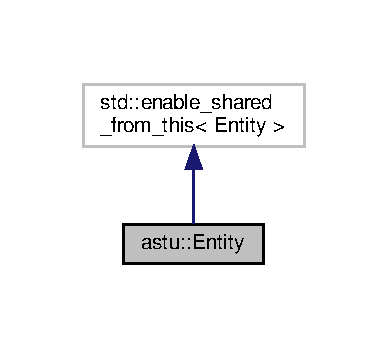
\includegraphics[width=186pt]{classastu_1_1Entity__inherit__graph}
\end{center}
\end{figure}


Collaboration diagram for astu\+:\+:Entity\+:\nopagebreak
\begin{figure}[H]
\begin{center}
\leavevmode
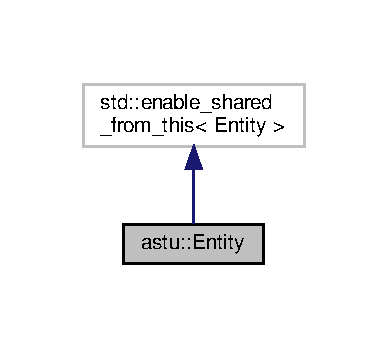
\includegraphics[width=186pt]{classastu_1_1Entity__coll__graph}
\end{center}
\end{figure}
\subsection*{Public Member Functions}
\begin{DoxyCompactItemize}
\item 
\hyperlink{classastu_1_1Entity_aed9aac4a995b5c044c0301302f2bd3d0}{Entity} ()
\item 
void \hyperlink{classastu_1_1Entity_ab8f47f4de88139f9202466b726e61aee}{Add\+Component} (std\+::shared\+\_\+ptr$<$ \hyperlink{classastu_1_1EntityComponent}{Entity\+Component} $>$ cmp)
\item 
bool \hyperlink{classastu_1_1Entity_ad1ee4a4e617de7c40eb252413b9045a1}{Has\+Component} (const std\+::type\+\_\+index \&type) const
\item 
\hyperlink{classastu_1_1EntityComponent}{Entity\+Component} \& \hyperlink{classastu_1_1Entity_a3d9bb583859f1a941fdaad76f5093323}{Get\+Component} (const std\+::type\+\_\+index \&type)
\item 
const \hyperlink{classastu_1_1EntityComponent}{Entity\+Component} \& \hyperlink{classastu_1_1Entity_affe49f8c35d5b067f06803e27243189a}{Get\+Component} (const std\+::type\+\_\+index \&type) const
\item 
{\footnotesize template$<$typename T $>$ }\\T \& \hyperlink{classastu_1_1Entity_aeabb500a719de29039dd0fad4ea553c4}{Get\+Component} ()
\item 
{\footnotesize template$<$typename T $>$ }\\bool \hyperlink{classastu_1_1Entity_a80b75df1873d23f79f050bc6a178cd4c}{Has\+Component} ()
\end{DoxyCompactItemize}


\subsection{Detailed Description}
An entity is a container for compoments. 

\subsection{Constructor \& Destructor Documentation}
\mbox{\Hypertarget{classastu_1_1Entity_aed9aac4a995b5c044c0301302f2bd3d0}\label{classastu_1_1Entity_aed9aac4a995b5c044c0301302f2bd3d0}} 
\index{astu\+::\+Entity@{astu\+::\+Entity}!Entity@{Entity}}
\index{Entity@{Entity}!astu\+::\+Entity@{astu\+::\+Entity}}
\subsubsection{\texorpdfstring{Entity()}{Entity()}}
{\footnotesize\ttfamily astu\+::\+Entity\+::\+Entity (\begin{DoxyParamCaption}{ }\end{DoxyParamCaption})\hspace{0.3cm}{\ttfamily [inline]}}

Constructor. 

\subsection{Member Function Documentation}
\mbox{\Hypertarget{classastu_1_1Entity_ab8f47f4de88139f9202466b726e61aee}\label{classastu_1_1Entity_ab8f47f4de88139f9202466b726e61aee}} 
\index{astu\+::\+Entity@{astu\+::\+Entity}!Add\+Component@{Add\+Component}}
\index{Add\+Component@{Add\+Component}!astu\+::\+Entity@{astu\+::\+Entity}}
\subsubsection{\texorpdfstring{Add\+Component()}{AddComponent()}}
{\footnotesize\ttfamily void astu\+::\+Entity\+::\+Add\+Component (\begin{DoxyParamCaption}\item[{std\+::shared\+\_\+ptr$<$ \hyperlink{classastu_1_1EntityComponent}{Entity\+Component} $>$}]{cmp }\end{DoxyParamCaption})}

Adds a component to this entity.


\begin{DoxyParams}{Parameters}
{\em cmp} & the component to add \\
\hline
\end{DoxyParams}
\mbox{\Hypertarget{classastu_1_1Entity_a3d9bb583859f1a941fdaad76f5093323}\label{classastu_1_1Entity_a3d9bb583859f1a941fdaad76f5093323}} 
\index{astu\+::\+Entity@{astu\+::\+Entity}!Get\+Component@{Get\+Component}}
\index{Get\+Component@{Get\+Component}!astu\+::\+Entity@{astu\+::\+Entity}}
\subsubsection{\texorpdfstring{Get\+Component()}{GetComponent()}\hspace{0.1cm}{\footnotesize\ttfamily [1/3]}}
{\footnotesize\ttfamily \hyperlink{classastu_1_1EntityComponent}{Entity\+Component}\& astu\+::\+Entity\+::\+Get\+Component (\begin{DoxyParamCaption}\item[{const std\+::type\+\_\+index \&}]{type }\end{DoxyParamCaption})}

Returns the component of a specific type.

This method is mainly used by the template method {\ttfamily get\+Component}, which is much more convenient to use because no type cast is required.

A dynamic cast is not necessary because this method ensures to return a component of the required type which can safely be casted using a fast static cast.

{\bfseries Usage example\+:} 
\begin{DoxyCode}
\textcolor{keyword}{auto} & pose = \textcolor{keyword}{static\_cast<}Pose2D &\textcolor{keyword}{>}( entity.getComponent( std::type\_index( \textcolor{keyword}{typeid}(Pose2D) ) ) );
\end{DoxyCode}



\begin{DoxyParams}{Parameters}
{\em type} & the component type \\
\hline
\end{DoxyParams}
\begin{DoxyReturn}{Returns}
the requested component 
\end{DoxyReturn}

\begin{DoxyExceptions}{Exceptions}
{\em std\+::logic\+\_\+error} & in case the requested component does not exist \\
\hline
\end{DoxyExceptions}
\mbox{\Hypertarget{classastu_1_1Entity_affe49f8c35d5b067f06803e27243189a}\label{classastu_1_1Entity_affe49f8c35d5b067f06803e27243189a}} 
\index{astu\+::\+Entity@{astu\+::\+Entity}!Get\+Component@{Get\+Component}}
\index{Get\+Component@{Get\+Component}!astu\+::\+Entity@{astu\+::\+Entity}}
\subsubsection{\texorpdfstring{Get\+Component()}{GetComponent()}\hspace{0.1cm}{\footnotesize\ttfamily [2/3]}}
{\footnotesize\ttfamily const \hyperlink{classastu_1_1EntityComponent}{Entity\+Component}\& astu\+::\+Entity\+::\+Get\+Component (\begin{DoxyParamCaption}\item[{const std\+::type\+\_\+index \&}]{type }\end{DoxyParamCaption}) const}

Returns the component of a specific type.

This is the constant version of this method. See the non-\/constant version description for details.


\begin{DoxyParams}{Parameters}
{\em type} & the component type \\
\hline
\end{DoxyParams}
\begin{DoxyReturn}{Returns}
the requested component 
\end{DoxyReturn}

\begin{DoxyExceptions}{Exceptions}
{\em std\+::logic\+\_\+error} & in case the requested component does not exist \\
\hline
\end{DoxyExceptions}
\mbox{\Hypertarget{classastu_1_1Entity_aeabb500a719de29039dd0fad4ea553c4}\label{classastu_1_1Entity_aeabb500a719de29039dd0fad4ea553c4}} 
\index{astu\+::\+Entity@{astu\+::\+Entity}!Get\+Component@{Get\+Component}}
\index{Get\+Component@{Get\+Component}!astu\+::\+Entity@{astu\+::\+Entity}}
\subsubsection{\texorpdfstring{Get\+Component()}{GetComponent()}\hspace{0.1cm}{\footnotesize\ttfamily [3/3]}}
{\footnotesize\ttfamily template$<$typename T $>$ \\
T\& astu\+::\+Entity\+::\+Get\+Component (\begin{DoxyParamCaption}{ }\end{DoxyParamCaption})\hspace{0.3cm}{\ttfamily [inline]}}

Retrieves the component a specifi type from this entity.

This template method offers a convenient way to retrieve a component by specifying the type of the component to retrieve as template parameter.

{\bfseries Usage example\+:} 
\begin{DoxyCode}
\textcolor{keyword}{auto} & pose = entity.getComponent<Pose2D>();
\end{DoxyCode}



\begin{DoxyTemplParams}{Template Parameters}
{\em T} & the type of the component to retrieve \\
\hline
\end{DoxyTemplParams}
\begin{DoxyReturn}{Returns}
the requested component 
\end{DoxyReturn}

\begin{DoxyExceptions}{Exceptions}
{\em std\+::logic\+\_\+error} & in case the requested component does not exist \\
\hline
\end{DoxyExceptions}
\mbox{\Hypertarget{classastu_1_1Entity_ad1ee4a4e617de7c40eb252413b9045a1}\label{classastu_1_1Entity_ad1ee4a4e617de7c40eb252413b9045a1}} 
\index{astu\+::\+Entity@{astu\+::\+Entity}!Has\+Component@{Has\+Component}}
\index{Has\+Component@{Has\+Component}!astu\+::\+Entity@{astu\+::\+Entity}}
\subsubsection{\texorpdfstring{Has\+Component()}{HasComponent()}\hspace{0.1cm}{\footnotesize\ttfamily [1/2]}}
{\footnotesize\ttfamily bool astu\+::\+Entity\+::\+Has\+Component (\begin{DoxyParamCaption}\item[{const std\+::type\+\_\+index \&}]{type }\end{DoxyParamCaption}) const}

Tests if specified type of component has been added to this entity.

This method is mainly used by the template method {\ttfamily Has\+Component}, which is more convenient to use.

This method requires a std\+::type\+\_\+index parameter to specify the type of component to be tested. The C++ {\ttfamily typeid} operator can be used to get the std\+::type\+\_\+info object, which will be automatically converted to a std\+::type\+\_\+index object when calling this method.

{\bfseries Usage example\+:} 
\begin{DoxyCode}
\textcolor{keywordflow}{if} ( entity.hasComponent( \textcolor{keyword}{typeid}(Pose2D) ) ) \{
    \textcolor{comment}{// do something with Pose2D component}
\}
\end{DoxyCode}



\begin{DoxyParams}{Parameters}
{\em type} & a type\+\_\+index specifying the type of component to test \\
\hline
\end{DoxyParams}
\begin{DoxyReturn}{Returns}
{\ttfamily true} if a component of the specified type exists 
\end{DoxyReturn}
\mbox{\Hypertarget{classastu_1_1Entity_a80b75df1873d23f79f050bc6a178cd4c}\label{classastu_1_1Entity_a80b75df1873d23f79f050bc6a178cd4c}} 
\index{astu\+::\+Entity@{astu\+::\+Entity}!Has\+Component@{Has\+Component}}
\index{Has\+Component@{Has\+Component}!astu\+::\+Entity@{astu\+::\+Entity}}
\subsubsection{\texorpdfstring{Has\+Component()}{HasComponent()}\hspace{0.1cm}{\footnotesize\ttfamily [2/2]}}
{\footnotesize\ttfamily template$<$typename T $>$ \\
bool astu\+::\+Entity\+::\+Has\+Component (\begin{DoxyParamCaption}{ }\end{DoxyParamCaption})\hspace{0.3cm}{\ttfamily [inline]}}

Tests whether a component of a specific type has been added to this entity.

This template method offers a convenient way to test if a certain component type exists in this entity by specifying the type of the component as template parameter.

{\bfseries Usage example\+:} 
\begin{DoxyCode}
\textcolor{keywordflow}{if} ( entity.hasComponent<Pose2D>() ) \{
    \textcolor{comment}{// do something with Pose2D component}
\}
\end{DoxyCode}



\begin{DoxyTemplParams}{Template Parameters}
{\em T} & the type of component to be tested \\
\hline
\end{DoxyTemplParams}
\begin{DoxyReturn}{Returns}
{\ttfamily true} if a component of the specified type exists 
\end{DoxyReturn}


The documentation for this class was generated from the following file\+:\begin{DoxyCompactItemize}
\item 
include/Entity\+Service.\+h\end{DoxyCompactItemize}

\hypertarget{classastu_1_1EntityComponent}{}\section{astu\+:\+:Entity\+Component Class Reference}
\label{classastu_1_1EntityComponent}\index{astu\+::\+Entity\+Component@{astu\+::\+Entity\+Component}}


{\ttfamily \#include $<$Entity\+Service.\+h$>$}

\subsection*{Public Member Functions}
\begin{DoxyCompactItemize}
\item 
\hyperlink{classastu_1_1EntityComponent_a9bb95d7ddc55093fd86e04d5b6aa98ec}{Entity\+Component} ()=default
\item 
virtual \hyperlink{classastu_1_1EntityComponent_a17295f763e201247c22bc677541646e5}{$\sim$\+Entity\+Component} ()
\end{DoxyCompactItemize}


\subsection{Detailed Description}
Base class for all entity components. 

\subsection{Constructor \& Destructor Documentation}
\mbox{\Hypertarget{classastu_1_1EntityComponent_a9bb95d7ddc55093fd86e04d5b6aa98ec}\label{classastu_1_1EntityComponent_a9bb95d7ddc55093fd86e04d5b6aa98ec}} 
\index{astu\+::\+Entity\+Component@{astu\+::\+Entity\+Component}!Entity\+Component@{Entity\+Component}}
\index{Entity\+Component@{Entity\+Component}!astu\+::\+Entity\+Component@{astu\+::\+Entity\+Component}}
\subsubsection{\texorpdfstring{Entity\+Component()}{EntityComponent()}}
{\footnotesize\ttfamily astu\+::\+Entity\+Component\+::\+Entity\+Component (\begin{DoxyParamCaption}{ }\end{DoxyParamCaption})\hspace{0.3cm}{\ttfamily [default]}}

Constructor. \mbox{\Hypertarget{classastu_1_1EntityComponent_a17295f763e201247c22bc677541646e5}\label{classastu_1_1EntityComponent_a17295f763e201247c22bc677541646e5}} 
\index{astu\+::\+Entity\+Component@{astu\+::\+Entity\+Component}!````~Entity\+Component@{$\sim$\+Entity\+Component}}
\index{````~Entity\+Component@{$\sim$\+Entity\+Component}!astu\+::\+Entity\+Component@{astu\+::\+Entity\+Component}}
\subsubsection{\texorpdfstring{$\sim$\+Entity\+Component()}{~EntityComponent()}}
{\footnotesize\ttfamily virtual astu\+::\+Entity\+Component\+::$\sim$\+Entity\+Component (\begin{DoxyParamCaption}{ }\end{DoxyParamCaption})\hspace{0.3cm}{\ttfamily [inline]}, {\ttfamily [virtual]}}

Virtual destructor. 

The documentation for this class was generated from the following file\+:\begin{DoxyCompactItemize}
\item 
include/Entity\+Service.\+h\end{DoxyCompactItemize}

\hypertarget{classastu_1_1EntityFamily}{}\section{astu\+:\+:Entity\+Family Class Reference}
\label{classastu_1_1EntityFamily}\index{astu\+::\+Entity\+Family@{astu\+::\+Entity\+Family}}


{\ttfamily \#include $<$Entity\+Service.\+h$>$}

\subsection*{Public Member Functions}
\begin{DoxyCompactItemize}
\item 
\mbox{\Hypertarget{classastu_1_1EntityFamily_a8452fd5df3f194dd8824b9ea88d426bf}\label{classastu_1_1EntityFamily_a8452fd5df3f194dd8824b9ea88d426bf}} 
bool {\bfseries Is\+Member} (const \hyperlink{classastu_1_1Entity}{Entity} \&entity) const
\item 
bool \hyperlink{classastu_1_1EntityFamily_ac2389d2f9807b3ebdb570f0fd8930957}{operator$<$} (const \hyperlink{classastu_1_1EntityFamily}{Entity\+Family} \&o) const
\end{DoxyCompactItemize}
\subsection*{Static Public Member Functions}
\begin{DoxyCompactItemize}
\item 
{\footnotesize template$<$typename ... Ts$>$ }\\static \hyperlink{classastu_1_1EntityFamily}{Entity\+Family} \hyperlink{classastu_1_1EntityFamily_ad201d4186eaef0f02c07a07889fc7763}{Create} ()
\end{DoxyCompactItemize}


\subsection{Detailed Description}
Describes entities which share a certain set of entity components. 

\subsection{Member Function Documentation}
\mbox{\Hypertarget{classastu_1_1EntityFamily_ad201d4186eaef0f02c07a07889fc7763}\label{classastu_1_1EntityFamily_ad201d4186eaef0f02c07a07889fc7763}} 
\index{astu\+::\+Entity\+Family@{astu\+::\+Entity\+Family}!Create@{Create}}
\index{Create@{Create}!astu\+::\+Entity\+Family@{astu\+::\+Entity\+Family}}
\subsubsection{\texorpdfstring{Create()}{Create()}}
{\footnotesize\ttfamily template$<$typename ... Ts$>$ \\
static \hyperlink{classastu_1_1EntityFamily}{Entity\+Family} astu\+::\+Entity\+Family\+::\+Create (\begin{DoxyParamCaption}{ }\end{DoxyParamCaption})\hspace{0.3cm}{\ttfamily [inline]}, {\ttfamily [static]}}

Creates a new entity family. This static factory method is the only way to construct entity families. The constructor of this class is private.

Example usage\+: 
\begin{DoxyCode}
EntityFamily myFamily = EntityFamily::create<Transform2D, ShapeVisual2D>();
\end{DoxyCode}



\begin{DoxyTemplParams}{Template Parameters}
{\em Ts} & list of components the requested entities should share \\
\hline
\end{DoxyTemplParams}
\begin{DoxyReturn}{Returns}
the entity family 
\end{DoxyReturn}
\mbox{\Hypertarget{classastu_1_1EntityFamily_ac2389d2f9807b3ebdb570f0fd8930957}\label{classastu_1_1EntityFamily_ac2389d2f9807b3ebdb570f0fd8930957}} 
\index{astu\+::\+Entity\+Family@{astu\+::\+Entity\+Family}!operator$<$@{operator$<$}}
\index{operator$<$@{operator$<$}!astu\+::\+Entity\+Family@{astu\+::\+Entity\+Family}}
\subsubsection{\texorpdfstring{operator$<$()}{operator<()}}
{\footnotesize\ttfamily bool astu\+::\+Entity\+Family\+::operator$<$ (\begin{DoxyParamCaption}\item[{const \hyperlink{classastu_1_1EntityFamily}{Entity\+Family} \&}]{o }\end{DoxyParamCaption}) const\hspace{0.3cm}{\ttfamily [inline]}}

Binary less operator.

This operator is required to work as key in a map container. The less operator induces a strict weak ordering of elements.


\begin{DoxyParams}{Parameters}
{\em o} & the other entity family (right hand side) \\
\hline
\end{DoxyParams}
\begin{DoxyReturn}{Returns}
{\ttfamily true} if this element is less than the given element. 
\end{DoxyReturn}


The documentation for this class was generated from the following file\+:\begin{DoxyCompactItemize}
\item 
include/Entity\+Service.\+h\end{DoxyCompactItemize}

\hypertarget{classastu_1_1EntityService}{}\section{astu\+:\+:Entity\+Service Class Reference}
\label{classastu_1_1EntityService}\index{astu\+::\+Entity\+Service@{astu\+::\+Entity\+Service}}


{\ttfamily \#include $<$Entity\+Service.\+h$>$}



Inheritance diagram for astu\+:\+:Entity\+Service\+:\nopagebreak
\begin{figure}[H]
\begin{center}
\leavevmode
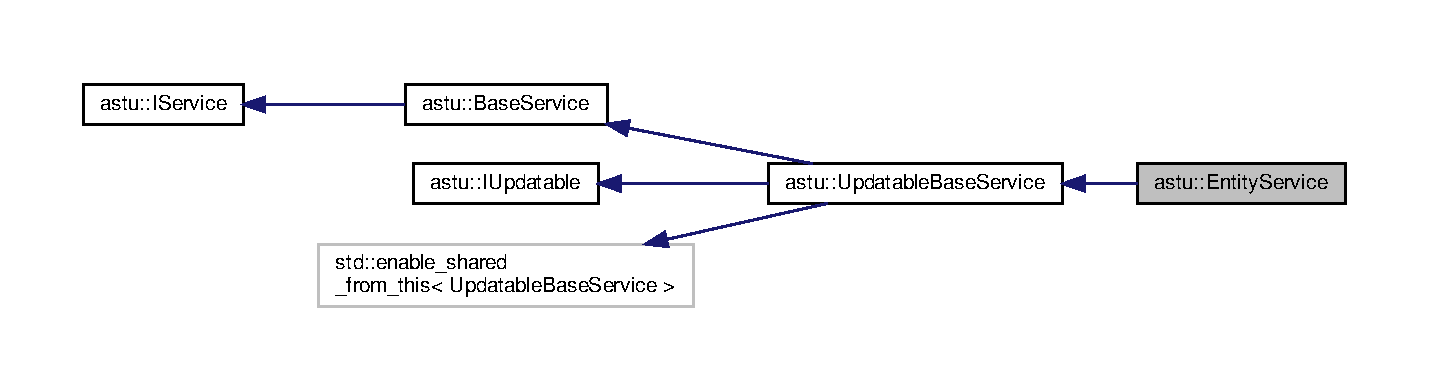
\includegraphics[width=262pt]{classastu_1_1EntityService__inherit__graph}
\end{center}
\end{figure}


Collaboration diagram for astu\+:\+:Entity\+Service\+:\nopagebreak
\begin{figure}[H]
\begin{center}
\leavevmode
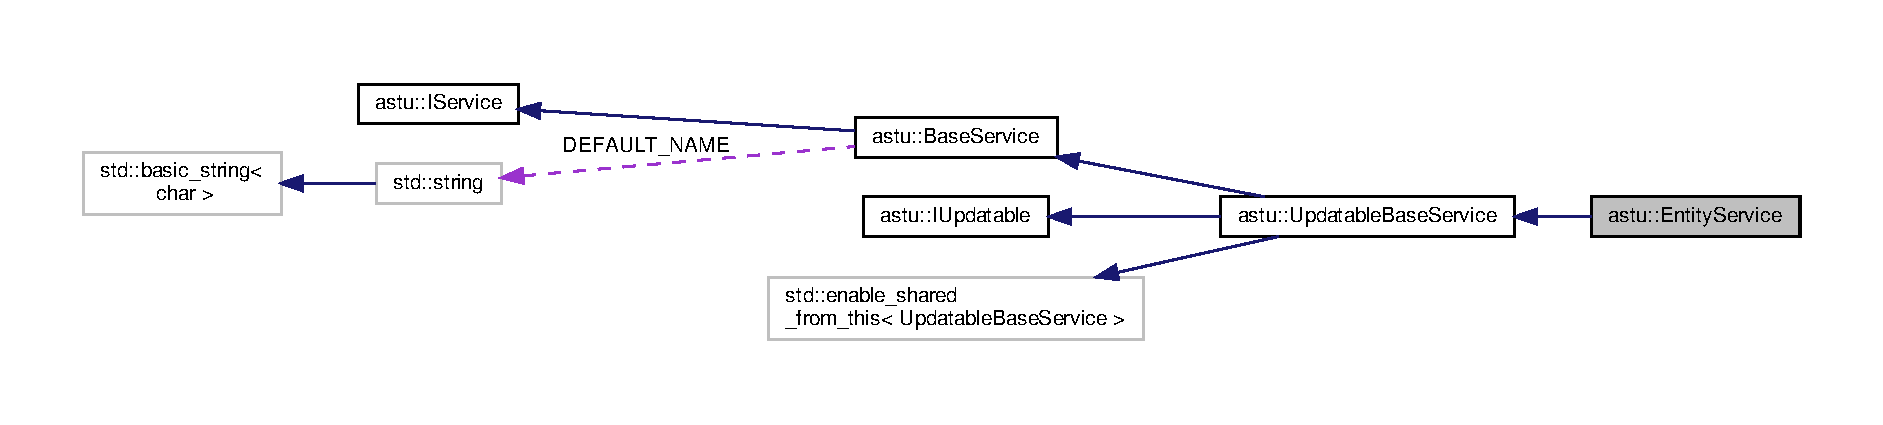
\includegraphics[width=309pt]{classastu_1_1EntityService__coll__graph}
\end{center}
\end{figure}
\subsection*{Public Member Functions}
\begin{DoxyCompactItemize}
\item 
\hyperlink{classastu_1_1EntityService_a74fc8d1e8b7aadf0899142c248cb2211}{Entity\+Service} (int update\+Priority=Priority\+::\+Normal)
\item 
void \hyperlink{classastu_1_1EntityService_ad6c6cb81dc8c48c7688f438571ee5da8}{Add\+Entity} (std\+::shared\+\_\+ptr$<$ \hyperlink{classastu_1_1Entity}{Entity} $>$ entity)
\item 
void \hyperlink{classastu_1_1EntityService_a748a71e470d5bb51bb650b15e0a78c63}{Remove\+Entity} (std\+::shared\+\_\+ptr$<$ \hyperlink{classastu_1_1Entity}{Entity} $>$ entity)
\item 
bool \hyperlink{classastu_1_1EntityService_a4a3c14fd7aa8edf4263913046744f277}{Has\+Entity} (std\+::shared\+\_\+ptr$<$ \hyperlink{classastu_1_1Entity}{Entity} $>$ entity) const
\item 
void \hyperlink{classastu_1_1EntityService_ac543fe51a3d1c9784bcab5775f5d388d}{Remove\+Entity} (\hyperlink{classastu_1_1Entity}{Entity} \&entity)
\item 
void \hyperlink{classastu_1_1EntityService_a1b21cf207324748c13c34568d3c1513e}{Remove\+All} ()
\item 
const std\+::shared\+\_\+ptr$<$ \hyperlink{group__ecs__group_gace2fb790b86c3908a65e4222f7ac2f4e}{Entity\+View} $>$ \hyperlink{classastu_1_1EntityService_aa295c07eb6a5c5321cf5820c9e41d008}{Get\+Entity\+View} (const \hyperlink{classastu_1_1EntityFamily}{Entity\+Family} \&family)
\item 
bool \hyperlink{classastu_1_1EntityService_a57fa7f62f90b8ecf4513045d7be9f15c}{Has\+Entity\+Listener} (const \hyperlink{classastu_1_1EntityFamily}{Entity\+Family} \&family, \hyperlink{classastu_1_1IEntityListener}{I\+Entity\+Listener} \&listener) const
\item 
void \hyperlink{classastu_1_1EntityService_ab338b1904b61dfe71c2b3bbcb390ada1}{Add\+Entity\+Listener} (const \hyperlink{classastu_1_1EntityFamily}{Entity\+Family} \&family, \hyperlink{classastu_1_1IEntityListener}{I\+Entity\+Listener} \&listener)
\item 
void \hyperlink{classastu_1_1EntityService_af9b12ecd243f0b0f98799fa2d147fecb}{Remove\+Entity\+Listener} (const \hyperlink{classastu_1_1EntityFamily}{Entity\+Family} \&family, \hyperlink{classastu_1_1IEntityListener}{I\+Entity\+Listener} \&listener)
\end{DoxyCompactItemize}
\subsection*{Protected Member Functions}
\begin{DoxyCompactItemize}
\item 
virtual void \hyperlink{classastu_1_1EntityService_a293ff7c8b84837b08cdabe98ed8a23ea}{On\+Startup} () override
\item 
virtual void \hyperlink{classastu_1_1EntityService_ac998c4d02a90460a129c8f2e0586d728}{On\+Shutdown} () override
\item 
virtual void \hyperlink{classastu_1_1EntityService_a70831a8dc185652c2c9056c4e3cc10e0}{On\+Update} () override
\end{DoxyCompactItemize}
\subsection*{Additional Inherited Members}


\subsection{Detailed Description}
The core service of the E\+CS, manages entities and entity listeners. 

\subsection{Constructor \& Destructor Documentation}
\mbox{\Hypertarget{classastu_1_1EntityService_a74fc8d1e8b7aadf0899142c248cb2211}\label{classastu_1_1EntityService_a74fc8d1e8b7aadf0899142c248cb2211}} 
\index{astu\+::\+Entity\+Service@{astu\+::\+Entity\+Service}!Entity\+Service@{Entity\+Service}}
\index{Entity\+Service@{Entity\+Service}!astu\+::\+Entity\+Service@{astu\+::\+Entity\+Service}}
\subsubsection{\texorpdfstring{Entity\+Service()}{EntityService()}}
{\footnotesize\ttfamily astu\+::\+Entity\+Service\+::\+Entity\+Service (\begin{DoxyParamCaption}\item[{int}]{update\+Priority = {\ttfamily Priority\+:\+:Normal} }\end{DoxyParamCaption})}

Constructor.


\begin{DoxyParams}{Parameters}
{\em update\+Priority} & the update priority of this service \\
\hline
\end{DoxyParams}


\subsection{Member Function Documentation}
\mbox{\Hypertarget{classastu_1_1EntityService_ad6c6cb81dc8c48c7688f438571ee5da8}\label{classastu_1_1EntityService_ad6c6cb81dc8c48c7688f438571ee5da8}} 
\index{astu\+::\+Entity\+Service@{astu\+::\+Entity\+Service}!Add\+Entity@{Add\+Entity}}
\index{Add\+Entity@{Add\+Entity}!astu\+::\+Entity\+Service@{astu\+::\+Entity\+Service}}
\subsubsection{\texorpdfstring{Add\+Entity()}{AddEntity()}}
{\footnotesize\ttfamily void astu\+::\+Entity\+Service\+::\+Add\+Entity (\begin{DoxyParamCaption}\item[{std\+::shared\+\_\+ptr$<$ \hyperlink{classastu_1_1Entity}{Entity} $>$}]{entity }\end{DoxyParamCaption})}

Adds an entity to this service.


\begin{DoxyParams}{Parameters}
{\em entity} & the entity to add \\
\hline
\end{DoxyParams}
\mbox{\Hypertarget{classastu_1_1EntityService_ab338b1904b61dfe71c2b3bbcb390ada1}\label{classastu_1_1EntityService_ab338b1904b61dfe71c2b3bbcb390ada1}} 
\index{astu\+::\+Entity\+Service@{astu\+::\+Entity\+Service}!Add\+Entity\+Listener@{Add\+Entity\+Listener}}
\index{Add\+Entity\+Listener@{Add\+Entity\+Listener}!astu\+::\+Entity\+Service@{astu\+::\+Entity\+Service}}
\subsubsection{\texorpdfstring{Add\+Entity\+Listener()}{AddEntityListener()}}
{\footnotesize\ttfamily void astu\+::\+Entity\+Service\+::\+Add\+Entity\+Listener (\begin{DoxyParamCaption}\item[{const \hyperlink{classastu_1_1EntityFamily}{Entity\+Family} \&}]{family,  }\item[{\hyperlink{classastu_1_1IEntityListener}{I\+Entity\+Listener} \&}]{listener }\end{DoxyParamCaption})}

Adds an entity listener to this service.


\begin{DoxyParams}{Parameters}
{\em family} & the entity family the listener is interested in \\
\hline
{\em listener} & the entity listener to add \\
\hline
\end{DoxyParams}
\mbox{\Hypertarget{classastu_1_1EntityService_aa295c07eb6a5c5321cf5820c9e41d008}\label{classastu_1_1EntityService_aa295c07eb6a5c5321cf5820c9e41d008}} 
\index{astu\+::\+Entity\+Service@{astu\+::\+Entity\+Service}!Get\+Entity\+View@{Get\+Entity\+View}}
\index{Get\+Entity\+View@{Get\+Entity\+View}!astu\+::\+Entity\+Service@{astu\+::\+Entity\+Service}}
\subsubsection{\texorpdfstring{Get\+Entity\+View()}{GetEntityView()}}
{\footnotesize\ttfamily const std\+::shared\+\_\+ptr$<$\hyperlink{group__ecs__group_gace2fb790b86c3908a65e4222f7ac2f4e}{Entity\+View}$>$ astu\+::\+Entity\+Service\+::\+Get\+Entity\+View (\begin{DoxyParamCaption}\item[{const \hyperlink{classastu_1_1EntityFamily}{Entity\+Family} \&}]{family }\end{DoxyParamCaption})}

Returns a view to a certain family of entities.

Any caller of this method can keep the returned pointer to the entity view. The view gets updated automatically when entities are added or removed.

\begin{DoxyReturn}{Returns}
the entity view 
\end{DoxyReturn}
\mbox{\Hypertarget{classastu_1_1EntityService_a4a3c14fd7aa8edf4263913046744f277}\label{classastu_1_1EntityService_a4a3c14fd7aa8edf4263913046744f277}} 
\index{astu\+::\+Entity\+Service@{astu\+::\+Entity\+Service}!Has\+Entity@{Has\+Entity}}
\index{Has\+Entity@{Has\+Entity}!astu\+::\+Entity\+Service@{astu\+::\+Entity\+Service}}
\subsubsection{\texorpdfstring{Has\+Entity()}{HasEntity()}}
{\footnotesize\ttfamily bool astu\+::\+Entity\+Service\+::\+Has\+Entity (\begin{DoxyParamCaption}\item[{std\+::shared\+\_\+ptr$<$ \hyperlink{classastu_1_1Entity}{Entity} $>$}]{entity }\end{DoxyParamCaption}) const}

Tests whether the specified entity exists.

\begin{DoxyReturn}{Returns}
{\ttfamily true} if the entity exists 
\end{DoxyReturn}
\mbox{\Hypertarget{classastu_1_1EntityService_a57fa7f62f90b8ecf4513045d7be9f15c}\label{classastu_1_1EntityService_a57fa7f62f90b8ecf4513045d7be9f15c}} 
\index{astu\+::\+Entity\+Service@{astu\+::\+Entity\+Service}!Has\+Entity\+Listener@{Has\+Entity\+Listener}}
\index{Has\+Entity\+Listener@{Has\+Entity\+Listener}!astu\+::\+Entity\+Service@{astu\+::\+Entity\+Service}}
\subsubsection{\texorpdfstring{Has\+Entity\+Listener()}{HasEntityListener()}}
{\footnotesize\ttfamily bool astu\+::\+Entity\+Service\+::\+Has\+Entity\+Listener (\begin{DoxyParamCaption}\item[{const \hyperlink{classastu_1_1EntityFamily}{Entity\+Family} \&}]{family,  }\item[{\hyperlink{classastu_1_1IEntityListener}{I\+Entity\+Listener} \&}]{listener }\end{DoxyParamCaption}) const}

Tests whether an entity listener has already been added.


\begin{DoxyParams}{Parameters}
{\em family} & the entity family the listener is interested in \\
\hline
{\em listener} & the entity listener to test \\
\hline
\end{DoxyParams}
\mbox{\Hypertarget{classastu_1_1EntityService_ac998c4d02a90460a129c8f2e0586d728}\label{classastu_1_1EntityService_ac998c4d02a90460a129c8f2e0586d728}} 
\index{astu\+::\+Entity\+Service@{astu\+::\+Entity\+Service}!On\+Shutdown@{On\+Shutdown}}
\index{On\+Shutdown@{On\+Shutdown}!astu\+::\+Entity\+Service@{astu\+::\+Entity\+Service}}
\subsubsection{\texorpdfstring{On\+Shutdown()}{OnShutdown()}}
{\footnotesize\ttfamily virtual void astu\+::\+Entity\+Service\+::\+On\+Shutdown (\begin{DoxyParamCaption}{ }\end{DoxyParamCaption})\hspace{0.3cm}{\ttfamily [override]}, {\ttfamily [protected]}, {\ttfamily [virtual]}}

Called by the service base method on shutdown.

Derived can override this method for de-\/initialization purposes, e.\+g., releasing resources, etc. 

Reimplemented from \hyperlink{classastu_1_1Service_a1e1dff727df791c57fae782d8a613c5f}{astu\+::\+Service}.

\mbox{\Hypertarget{classastu_1_1EntityService_a293ff7c8b84837b08cdabe98ed8a23ea}\label{classastu_1_1EntityService_a293ff7c8b84837b08cdabe98ed8a23ea}} 
\index{astu\+::\+Entity\+Service@{astu\+::\+Entity\+Service}!On\+Startup@{On\+Startup}}
\index{On\+Startup@{On\+Startup}!astu\+::\+Entity\+Service@{astu\+::\+Entity\+Service}}
\subsubsection{\texorpdfstring{On\+Startup()}{OnStartup()}}
{\footnotesize\ttfamily virtual void astu\+::\+Entity\+Service\+::\+On\+Startup (\begin{DoxyParamCaption}{ }\end{DoxyParamCaption})\hspace{0.3cm}{\ttfamily [override]}, {\ttfamily [protected]}, {\ttfamily [virtual]}}

Called by the service base class on startup.

Derived can override this method for initialization purposes. 

Reimplemented from \hyperlink{classastu_1_1Service_a357dc663e000b1f086f681ec3c459bfe}{astu\+::\+Service}.

\mbox{\Hypertarget{classastu_1_1EntityService_a70831a8dc185652c2c9056c4e3cc10e0}\label{classastu_1_1EntityService_a70831a8dc185652c2c9056c4e3cc10e0}} 
\index{astu\+::\+Entity\+Service@{astu\+::\+Entity\+Service}!On\+Update@{On\+Update}}
\index{On\+Update@{On\+Update}!astu\+::\+Entity\+Service@{astu\+::\+Entity\+Service}}
\subsubsection{\texorpdfstring{On\+Update()}{OnUpdate()}}
{\footnotesize\ttfamily virtual void astu\+::\+Entity\+Service\+::\+On\+Update (\begin{DoxyParamCaption}{ }\end{DoxyParamCaption})\hspace{0.3cm}{\ttfamily [override]}, {\ttfamily [protected]}, {\ttfamily [virtual]}}

Called when an update is due. 

Reimplemented from \hyperlink{classastu_1_1Updatable_a925566c9770b95895c6c7294f9d51528}{astu\+::\+Updatable}.

\mbox{\Hypertarget{classastu_1_1EntityService_a1b21cf207324748c13c34568d3c1513e}\label{classastu_1_1EntityService_a1b21cf207324748c13c34568d3c1513e}} 
\index{astu\+::\+Entity\+Service@{astu\+::\+Entity\+Service}!Remove\+All@{Remove\+All}}
\index{Remove\+All@{Remove\+All}!astu\+::\+Entity\+Service@{astu\+::\+Entity\+Service}}
\subsubsection{\texorpdfstring{Remove\+All()}{RemoveAll()}}
{\footnotesize\ttfamily void astu\+::\+Entity\+Service\+::\+Remove\+All (\begin{DoxyParamCaption}{ }\end{DoxyParamCaption})}

Removes all entities. \mbox{\Hypertarget{classastu_1_1EntityService_a748a71e470d5bb51bb650b15e0a78c63}\label{classastu_1_1EntityService_a748a71e470d5bb51bb650b15e0a78c63}} 
\index{astu\+::\+Entity\+Service@{astu\+::\+Entity\+Service}!Remove\+Entity@{Remove\+Entity}}
\index{Remove\+Entity@{Remove\+Entity}!astu\+::\+Entity\+Service@{astu\+::\+Entity\+Service}}
\subsubsection{\texorpdfstring{Remove\+Entity()}{RemoveEntity()}\hspace{0.1cm}{\footnotesize\ttfamily [1/2]}}
{\footnotesize\ttfamily void astu\+::\+Entity\+Service\+::\+Remove\+Entity (\begin{DoxyParamCaption}\item[{std\+::shared\+\_\+ptr$<$ \hyperlink{classastu_1_1Entity}{Entity} $>$}]{entity }\end{DoxyParamCaption})}

Removes an entity from this service.


\begin{DoxyParams}{Parameters}
{\em entity} & the entity to remove \\
\hline
\end{DoxyParams}
\mbox{\Hypertarget{classastu_1_1EntityService_ac543fe51a3d1c9784bcab5775f5d388d}\label{classastu_1_1EntityService_ac543fe51a3d1c9784bcab5775f5d388d}} 
\index{astu\+::\+Entity\+Service@{astu\+::\+Entity\+Service}!Remove\+Entity@{Remove\+Entity}}
\index{Remove\+Entity@{Remove\+Entity}!astu\+::\+Entity\+Service@{astu\+::\+Entity\+Service}}
\subsubsection{\texorpdfstring{Remove\+Entity()}{RemoveEntity()}\hspace{0.1cm}{\footnotesize\ttfamily [2/2]}}
{\footnotesize\ttfamily void astu\+::\+Entity\+Service\+::\+Remove\+Entity (\begin{DoxyParamCaption}\item[{\hyperlink{classastu_1_1Entity}{Entity} \&}]{entity }\end{DoxyParamCaption})\hspace{0.3cm}{\ttfamily [inline]}}

Removes an entity from this service.


\begin{DoxyParams}{Parameters}
{\em entity} & the entity to remove \\
\hline
\end{DoxyParams}
\mbox{\Hypertarget{classastu_1_1EntityService_af9b12ecd243f0b0f98799fa2d147fecb}\label{classastu_1_1EntityService_af9b12ecd243f0b0f98799fa2d147fecb}} 
\index{astu\+::\+Entity\+Service@{astu\+::\+Entity\+Service}!Remove\+Entity\+Listener@{Remove\+Entity\+Listener}}
\index{Remove\+Entity\+Listener@{Remove\+Entity\+Listener}!astu\+::\+Entity\+Service@{astu\+::\+Entity\+Service}}
\subsubsection{\texorpdfstring{Remove\+Entity\+Listener()}{RemoveEntityListener()}}
{\footnotesize\ttfamily void astu\+::\+Entity\+Service\+::\+Remove\+Entity\+Listener (\begin{DoxyParamCaption}\item[{const \hyperlink{classastu_1_1EntityFamily}{Entity\+Family} \&}]{family,  }\item[{\hyperlink{classastu_1_1IEntityListener}{I\+Entity\+Listener} \&}]{listener }\end{DoxyParamCaption})}

Removes an entity listener to from service.


\begin{DoxyParams}{Parameters}
{\em family} & the entity family the listener is interested in \\
\hline
{\em listener} & the entity listener to remove \\
\hline
\end{DoxyParams}


The documentation for this class was generated from the following file\+:\begin{DoxyCompactItemize}
\item 
include/\+E\+C\+S/Entity\+Service.\+h\end{DoxyCompactItemize}

\hypertarget{classastu_1_1IEntityListener}{}\section{astu\+:\+:I\+Entity\+Listener Class Reference}
\label{classastu_1_1IEntityListener}\index{astu\+::\+I\+Entity\+Listener@{astu\+::\+I\+Entity\+Listener}}


{\ttfamily \#include $<$Entity\+Service.\+h$>$}



Inheritance diagram for astu\+:\+:I\+Entity\+Listener\+:\nopagebreak
\begin{figure}[H]
\begin{center}
\leavevmode
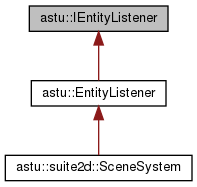
\includegraphics[width=220pt]{classastu_1_1IEntityListener__inherit__graph}
\end{center}
\end{figure}
\subsection*{Public Member Functions}
\begin{DoxyCompactItemize}
\item 
virtual \hyperlink{classastu_1_1IEntityListener_ad3e01cd267ff128c2176d06897c8c7b6}{$\sim$\+I\+Entity\+Listener} ()
\item 
virtual void \hyperlink{classastu_1_1IEntityListener_afa087302fdf0bd999297b0d35ceb1f61}{On\+Entity\+Added} (std\+::shared\+\_\+ptr$<$ \hyperlink{classastu_1_1Entity}{astu\+::\+Entity} $>$ entity)=0
\item 
virtual void \hyperlink{classastu_1_1IEntityListener_ab3d5a276da5e42cc4831e747fdf11718}{On\+Entity\+Removed} (std\+::shared\+\_\+ptr$<$ \hyperlink{classastu_1_1Entity}{astu\+::\+Entity} $>$ entity)=0
\end{DoxyCompactItemize}


\subsection{Detailed Description}
Interface for entity listeners which get informed when entities get added or removed. 

\subsection{Constructor \& Destructor Documentation}
\mbox{\Hypertarget{classastu_1_1IEntityListener_ad3e01cd267ff128c2176d06897c8c7b6}\label{classastu_1_1IEntityListener_ad3e01cd267ff128c2176d06897c8c7b6}} 
\index{astu\+::\+I\+Entity\+Listener@{astu\+::\+I\+Entity\+Listener}!````~I\+Entity\+Listener@{$\sim$\+I\+Entity\+Listener}}
\index{````~I\+Entity\+Listener@{$\sim$\+I\+Entity\+Listener}!astu\+::\+I\+Entity\+Listener@{astu\+::\+I\+Entity\+Listener}}
\subsubsection{\texorpdfstring{$\sim$\+I\+Entity\+Listener()}{~IEntityListener()}}
{\footnotesize\ttfamily virtual astu\+::\+I\+Entity\+Listener\+::$\sim$\+I\+Entity\+Listener (\begin{DoxyParamCaption}{ }\end{DoxyParamCaption})\hspace{0.3cm}{\ttfamily [inline]}, {\ttfamily [virtual]}}

Virtual destructor. 

\subsection{Member Function Documentation}
\mbox{\Hypertarget{classastu_1_1IEntityListener_afa087302fdf0bd999297b0d35ceb1f61}\label{classastu_1_1IEntityListener_afa087302fdf0bd999297b0d35ceb1f61}} 
\index{astu\+::\+I\+Entity\+Listener@{astu\+::\+I\+Entity\+Listener}!On\+Entity\+Added@{On\+Entity\+Added}}
\index{On\+Entity\+Added@{On\+Entity\+Added}!astu\+::\+I\+Entity\+Listener@{astu\+::\+I\+Entity\+Listener}}
\subsubsection{\texorpdfstring{On\+Entity\+Added()}{OnEntityAdded()}}
{\footnotesize\ttfamily virtual void astu\+::\+I\+Entity\+Listener\+::\+On\+Entity\+Added (\begin{DoxyParamCaption}\item[{std\+::shared\+\_\+ptr$<$ \hyperlink{classastu_1_1Entity}{astu\+::\+Entity} $>$}]{entity }\end{DoxyParamCaption})\hspace{0.3cm}{\ttfamily [pure virtual]}}

Called when an entity has been added.


\begin{DoxyParams}{Parameters}
{\em entity} & the entity which has been added \\
\hline
\end{DoxyParams}


Implemented in \hyperlink{classastu_1_1EntityListener_a0c123b57dcabc4c2b6cee8f05db545c8}{astu\+::\+Entity\+Listener}.

\mbox{\Hypertarget{classastu_1_1IEntityListener_ab3d5a276da5e42cc4831e747fdf11718}\label{classastu_1_1IEntityListener_ab3d5a276da5e42cc4831e747fdf11718}} 
\index{astu\+::\+I\+Entity\+Listener@{astu\+::\+I\+Entity\+Listener}!On\+Entity\+Removed@{On\+Entity\+Removed}}
\index{On\+Entity\+Removed@{On\+Entity\+Removed}!astu\+::\+I\+Entity\+Listener@{astu\+::\+I\+Entity\+Listener}}
\subsubsection{\texorpdfstring{On\+Entity\+Removed()}{OnEntityRemoved()}}
{\footnotesize\ttfamily virtual void astu\+::\+I\+Entity\+Listener\+::\+On\+Entity\+Removed (\begin{DoxyParamCaption}\item[{std\+::shared\+\_\+ptr$<$ \hyperlink{classastu_1_1Entity}{astu\+::\+Entity} $>$}]{entity }\end{DoxyParamCaption})\hspace{0.3cm}{\ttfamily [pure virtual]}}

Called when an entity has been removed.


\begin{DoxyParams}{Parameters}
{\em entity} & the entity which has been removed \\
\hline
\end{DoxyParams}


Implemented in \hyperlink{classastu_1_1EntityListener_ae380d941fafd6933a9f290ac50e7f32b}{astu\+::\+Entity\+Listener}.



The documentation for this class was generated from the following file\+:\begin{DoxyCompactItemize}
\item 
include/\+E\+C\+S/Entity\+Service.\+h\end{DoxyCompactItemize}

\hypertarget{classastu_1_1Image}{}\section{astu\+:\+:Image Class Reference}
\label{classastu_1_1Image}\index{astu\+::\+Image@{astu\+::\+Image}}


{\ttfamily \#include $<$Image.\+h$>$}

\subsection*{Public Member Functions}
\begin{DoxyCompactItemize}
\item 
\hyperlink{classastu_1_1Image_a930c3dfe86d60d209199cf27d2102446}{Image} (int w, int h)
\item 
int \hyperlink{classastu_1_1Image_a654888b88e109da1099ade3ec54f0520}{Get\+Width} () const
\item 
int \hyperlink{classastu_1_1Image_ad64d3b2abc18e54ba8beb4e212a75a10}{Get\+Height} () const
\item 
double \hyperlink{classastu_1_1Image_a06bdd931e5090f1eca62bd305b83cfd5}{Get\+Aspect\+Ratio} () const
\item 
const \hyperlink{classastu_1_1Color}{Color} \& \hyperlink{classastu_1_1Image_a8a31850315f2c74bc90627f4a292a10d}{Get\+Pixel} (int x, int y) const
\item 
void \hyperlink{classastu_1_1Image_a3c4770367d30abf8cefaa5cf777501a4}{Set\+Pixel} (int x, int y, const \hyperlink{classastu_1_1Color}{Color} \&c)
\item 
const \hyperlink{classastu_1_1Color}{Color} \& \hyperlink{classastu_1_1Image_a0ff83b1620356fdbe3ee3771d8a3ddb2}{Get\+Pixel} (size\+\_\+t idx) const
\item 
void \hyperlink{classastu_1_1Image_a1c2f1673fbba03abc50101c2d75ef12e}{Set\+Pixel} (size\+\_\+t idx, const \hyperlink{classastu_1_1Color}{Color} \&c)
\item 
size\+\_\+t \hyperlink{classastu_1_1Image_a53c53ecc0210786efa7f514966ad406b}{Number\+Of\+Pixels} () const
\item 
\hyperlink{classastu_1_1Color}{Color} $\ast$ \hyperlink{classastu_1_1Image_a3ce797d40010a7536662562c5f2e52da}{Get\+Pixels} ()
\item 
const \hyperlink{classastu_1_1Color}{Color} $\ast$ \hyperlink{classastu_1_1Image_ad2f3de6cc397bbc924c3718e54b1182f}{Get\+Pixels} () const
\end{DoxyCompactItemize}


\subsection{Detailed Description}
This class represents an image where each individual pixel is represented as instances of the class \hyperlink{classastu_1_1Color}{Color}. The \hyperlink{classastu_1_1Color}{Color} class represents a pixel as R\+G\+BA (red, green, blue and alpha channel) floating-\/point components.

Representing an image this way offers a convenient and straightforward way and maintains high color precision. However, memory consumption and performance might suffer. This class is preferably used for image synthesis and analysis. 

\subsection{Constructor \& Destructor Documentation}
\mbox{\Hypertarget{classastu_1_1Image_a930c3dfe86d60d209199cf27d2102446}\label{classastu_1_1Image_a930c3dfe86d60d209199cf27d2102446}} 
\index{astu\+::\+Image@{astu\+::\+Image}!Image@{Image}}
\index{Image@{Image}!astu\+::\+Image@{astu\+::\+Image}}
\subsubsection{\texorpdfstring{Image()}{Image()}}
{\footnotesize\ttfamily astu\+::\+Image\+::\+Image (\begin{DoxyParamCaption}\item[{int}]{w,  }\item[{int}]{h }\end{DoxyParamCaption})}

Constructor.


\begin{DoxyParams}{Parameters}
{\em w} & the width of the image in pixels \\
\hline
{\em h} & the height of the image in pixels \\
\hline
\end{DoxyParams}

\begin{DoxyExceptions}{Exceptions}
{\em std\+::domain\+\_\+error} & in case the width or height is \\
\hline
\end{DoxyExceptions}


\subsection{Member Function Documentation}
\mbox{\Hypertarget{classastu_1_1Image_a06bdd931e5090f1eca62bd305b83cfd5}\label{classastu_1_1Image_a06bdd931e5090f1eca62bd305b83cfd5}} 
\index{astu\+::\+Image@{astu\+::\+Image}!Get\+Aspect\+Ratio@{Get\+Aspect\+Ratio}}
\index{Get\+Aspect\+Ratio@{Get\+Aspect\+Ratio}!astu\+::\+Image@{astu\+::\+Image}}
\subsubsection{\texorpdfstring{Get\+Aspect\+Ratio()}{GetAspectRatio()}}
{\footnotesize\ttfamily double astu\+::\+Image\+::\+Get\+Aspect\+Ratio (\begin{DoxyParamCaption}{ }\end{DoxyParamCaption}) const\hspace{0.3cm}{\ttfamily [inline]}}

Returns the aspect ratio of this image.

\begin{DoxyReturn}{Returns}
the aspect ratio 
\end{DoxyReturn}
\mbox{\Hypertarget{classastu_1_1Image_ad64d3b2abc18e54ba8beb4e212a75a10}\label{classastu_1_1Image_ad64d3b2abc18e54ba8beb4e212a75a10}} 
\index{astu\+::\+Image@{astu\+::\+Image}!Get\+Height@{Get\+Height}}
\index{Get\+Height@{Get\+Height}!astu\+::\+Image@{astu\+::\+Image}}
\subsubsection{\texorpdfstring{Get\+Height()}{GetHeight()}}
{\footnotesize\ttfamily int astu\+::\+Image\+::\+Get\+Height (\begin{DoxyParamCaption}{ }\end{DoxyParamCaption}) const\hspace{0.3cm}{\ttfamily [inline]}}

Returns the height of this image

\begin{DoxyReturn}{Returns}
the height of this image in pixel 
\end{DoxyReturn}
\mbox{\Hypertarget{classastu_1_1Image_a8a31850315f2c74bc90627f4a292a10d}\label{classastu_1_1Image_a8a31850315f2c74bc90627f4a292a10d}} 
\index{astu\+::\+Image@{astu\+::\+Image}!Get\+Pixel@{Get\+Pixel}}
\index{Get\+Pixel@{Get\+Pixel}!astu\+::\+Image@{astu\+::\+Image}}
\subsubsection{\texorpdfstring{Get\+Pixel()}{GetPixel()}\hspace{0.1cm}{\footnotesize\ttfamily [1/2]}}
{\footnotesize\ttfamily const \hyperlink{classastu_1_1Color}{Color}\& astu\+::\+Image\+::\+Get\+Pixel (\begin{DoxyParamCaption}\item[{int}]{x,  }\item[{int}]{y }\end{DoxyParamCaption}) const}

Returns the color of a pixel.


\begin{DoxyParams}{Parameters}
{\em x} & the x-\/coordinate of the pixel \\
\hline
{\em y} & the y-\/coordinate of the pixel \\
\hline
\end{DoxyParams}
\begin{DoxyReturn}{Returns}
the color at the specified location 
\end{DoxyReturn}

\begin{DoxyExceptions}{Exceptions}
{\em std\+::out\+\_\+of\+\_\+range} & in case the coordinates are invalid \\
\hline
\end{DoxyExceptions}
\mbox{\Hypertarget{classastu_1_1Image_a0ff83b1620356fdbe3ee3771d8a3ddb2}\label{classastu_1_1Image_a0ff83b1620356fdbe3ee3771d8a3ddb2}} 
\index{astu\+::\+Image@{astu\+::\+Image}!Get\+Pixel@{Get\+Pixel}}
\index{Get\+Pixel@{Get\+Pixel}!astu\+::\+Image@{astu\+::\+Image}}
\subsubsection{\texorpdfstring{Get\+Pixel()}{GetPixel()}\hspace{0.1cm}{\footnotesize\ttfamily [2/2]}}
{\footnotesize\ttfamily const \hyperlink{classastu_1_1Color}{Color}\& astu\+::\+Image\+::\+Get\+Pixel (\begin{DoxyParamCaption}\item[{size\+\_\+t}]{idx }\end{DoxyParamCaption}) const}

Returns the color of a pixel.


\begin{DoxyParams}{Parameters}
{\em idx} & the linear index of the pixel \\
\hline
\end{DoxyParams}
\begin{DoxyReturn}{Returns}
the color of the pixel at the specified location 
\end{DoxyReturn}

\begin{DoxyExceptions}{Exceptions}
{\em std\+::out\+\_\+of\+\_\+range} & in case the index is invalid \\
\hline
\end{DoxyExceptions}
\mbox{\Hypertarget{classastu_1_1Image_a3ce797d40010a7536662562c5f2e52da}\label{classastu_1_1Image_a3ce797d40010a7536662562c5f2e52da}} 
\index{astu\+::\+Image@{astu\+::\+Image}!Get\+Pixels@{Get\+Pixels}}
\index{Get\+Pixels@{Get\+Pixels}!astu\+::\+Image@{astu\+::\+Image}}
\subsubsection{\texorpdfstring{Get\+Pixels()}{GetPixels()}\hspace{0.1cm}{\footnotesize\ttfamily [1/2]}}
{\footnotesize\ttfamily \hyperlink{classastu_1_1Color}{Color}$\ast$ astu\+::\+Image\+::\+Get\+Pixels (\begin{DoxyParamCaption}{ }\end{DoxyParamCaption})}

This method provides raw access to the pixel colors, use with care.

\begin{DoxyReturn}{Returns}
pointer to the linear array of pixel colors 
\end{DoxyReturn}
\mbox{\Hypertarget{classastu_1_1Image_ad2f3de6cc397bbc924c3718e54b1182f}\label{classastu_1_1Image_ad2f3de6cc397bbc924c3718e54b1182f}} 
\index{astu\+::\+Image@{astu\+::\+Image}!Get\+Pixels@{Get\+Pixels}}
\index{Get\+Pixels@{Get\+Pixels}!astu\+::\+Image@{astu\+::\+Image}}
\subsubsection{\texorpdfstring{Get\+Pixels()}{GetPixels()}\hspace{0.1cm}{\footnotesize\ttfamily [2/2]}}
{\footnotesize\ttfamily const \hyperlink{classastu_1_1Color}{Color}$\ast$ astu\+::\+Image\+::\+Get\+Pixels (\begin{DoxyParamCaption}{ }\end{DoxyParamCaption}) const}

This method provides raw access to the pixel colors, use with care.

This version returns a const pointer to the array and does not allow the modify the color values.

\begin{DoxyReturn}{Returns}
pointer to the linear array of pixel colors 
\end{DoxyReturn}
\mbox{\Hypertarget{classastu_1_1Image_a654888b88e109da1099ade3ec54f0520}\label{classastu_1_1Image_a654888b88e109da1099ade3ec54f0520}} 
\index{astu\+::\+Image@{astu\+::\+Image}!Get\+Width@{Get\+Width}}
\index{Get\+Width@{Get\+Width}!astu\+::\+Image@{astu\+::\+Image}}
\subsubsection{\texorpdfstring{Get\+Width()}{GetWidth()}}
{\footnotesize\ttfamily int astu\+::\+Image\+::\+Get\+Width (\begin{DoxyParamCaption}{ }\end{DoxyParamCaption}) const\hspace{0.3cm}{\ttfamily [inline]}}

Returns the width of this image

\begin{DoxyReturn}{Returns}
the width of this image in pixel 
\end{DoxyReturn}
\mbox{\Hypertarget{classastu_1_1Image_a53c53ecc0210786efa7f514966ad406b}\label{classastu_1_1Image_a53c53ecc0210786efa7f514966ad406b}} 
\index{astu\+::\+Image@{astu\+::\+Image}!Number\+Of\+Pixels@{Number\+Of\+Pixels}}
\index{Number\+Of\+Pixels@{Number\+Of\+Pixels}!astu\+::\+Image@{astu\+::\+Image}}
\subsubsection{\texorpdfstring{Number\+Of\+Pixels()}{NumberOfPixels()}}
{\footnotesize\ttfamily size\+\_\+t astu\+::\+Image\+::\+Number\+Of\+Pixels (\begin{DoxyParamCaption}{ }\end{DoxyParamCaption}) const}

Returns the number of pixels of this image.

The number of pixels equals width times height of this image.

\begin{DoxyReturn}{Returns}
the number of pixels 
\end{DoxyReturn}
\mbox{\Hypertarget{classastu_1_1Image_a3c4770367d30abf8cefaa5cf777501a4}\label{classastu_1_1Image_a3c4770367d30abf8cefaa5cf777501a4}} 
\index{astu\+::\+Image@{astu\+::\+Image}!Set\+Pixel@{Set\+Pixel}}
\index{Set\+Pixel@{Set\+Pixel}!astu\+::\+Image@{astu\+::\+Image}}
\subsubsection{\texorpdfstring{Set\+Pixel()}{SetPixel()}\hspace{0.1cm}{\footnotesize\ttfamily [1/2]}}
{\footnotesize\ttfamily void astu\+::\+Image\+::\+Set\+Pixel (\begin{DoxyParamCaption}\item[{int}]{x,  }\item[{int}]{y,  }\item[{const \hyperlink{classastu_1_1Color}{Color} \&}]{c }\end{DoxyParamCaption})}

Sets the color of a pixel.


\begin{DoxyParams}{Parameters}
{\em x} & the x-\/coordinate of the pixel \\
\hline
{\em y} & the y-\/coordinate of the pixel \\
\hline
{\em c} & the new color \\
\hline
\end{DoxyParams}

\begin{DoxyExceptions}{Exceptions}
{\em std\+::out\+\_\+of\+\_\+range} & in case the coordinates are invalid \\
\hline
\end{DoxyExceptions}
\mbox{\Hypertarget{classastu_1_1Image_a1c2f1673fbba03abc50101c2d75ef12e}\label{classastu_1_1Image_a1c2f1673fbba03abc50101c2d75ef12e}} 
\index{astu\+::\+Image@{astu\+::\+Image}!Set\+Pixel@{Set\+Pixel}}
\index{Set\+Pixel@{Set\+Pixel}!astu\+::\+Image@{astu\+::\+Image}}
\subsubsection{\texorpdfstring{Set\+Pixel()}{SetPixel()}\hspace{0.1cm}{\footnotesize\ttfamily [2/2]}}
{\footnotesize\ttfamily void astu\+::\+Image\+::\+Set\+Pixel (\begin{DoxyParamCaption}\item[{size\+\_\+t}]{idx,  }\item[{const \hyperlink{classastu_1_1Color}{Color} \&}]{c }\end{DoxyParamCaption})}

Sets the color of a pixel.


\begin{DoxyParams}{Parameters}
{\em idx} & the linear index of the pixel \\
\hline
{\em c} & the new color of the pixel at the specified location \\
\hline
\end{DoxyParams}

\begin{DoxyExceptions}{Exceptions}
{\em std\+::out\+\_\+of\+\_\+range} & in case the index is invalid \\
\hline
\end{DoxyExceptions}


The documentation for this class was generated from the following file\+:\begin{DoxyCompactItemize}
\item 
include/Image.\+h\end{DoxyCompactItemize}

\hypertarget{classastu_1_1ISdlRenderLayer}{}\section{astu\+:\+:I\+Sdl\+Render\+Layer Class Reference}
\label{classastu_1_1ISdlRenderLayer}\index{astu\+::\+I\+Sdl\+Render\+Layer@{astu\+::\+I\+Sdl\+Render\+Layer}}


{\ttfamily \#include $<$Sdl\+Render\+Service.\+h$>$}



Inheritance diagram for astu\+:\+:I\+Sdl\+Render\+Layer\+:\nopagebreak
\begin{figure}[H]
\begin{center}
\leavevmode
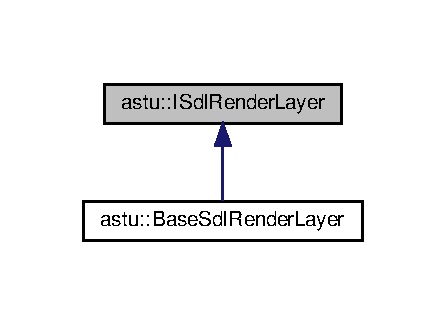
\includegraphics[width=214pt]{classastu_1_1ISdlRenderLayer__inherit__graph}
\end{center}
\end{figure}
\subsection*{Public Member Functions}
\begin{DoxyCompactItemize}
\item 
\hyperlink{classastu_1_1ISdlRenderLayer_af507055c193d430822d5aadb6cbaf6a9}{$\sim$\+I\+Sdl\+Render\+Layer} ()
\item 
virtual void \hyperlink{classastu_1_1ISdlRenderLayer_a18af53e17e7f6f945817ad3e8b8ecc87}{On\+Render} (S\+D\+L\+\_\+\+Renderer $\ast$renderer)=0
\item 
virtual void \hyperlink{classastu_1_1ISdlRenderLayer_abcded808a2405e1e59413b5d1f981f13}{On\+Resize} (int width, int height)=0
\item 
virtual int \hyperlink{classastu_1_1ISdlRenderLayer_a623b411a1afa967bdaa879f5075eec43}{Get\+Render\+Priority} () const =0
\end{DoxyCompactItemize}


\subsection{Detailed Description}
Interface for S\+D\+L-\/based renderer layers.

This inteface for render layers is using the hardware accelerated 2D render-\/mechanism of S\+DL. 

\subsection{Constructor \& Destructor Documentation}
\mbox{\Hypertarget{classastu_1_1ISdlRenderLayer_af507055c193d430822d5aadb6cbaf6a9}\label{classastu_1_1ISdlRenderLayer_af507055c193d430822d5aadb6cbaf6a9}} 
\index{astu\+::\+I\+Sdl\+Render\+Layer@{astu\+::\+I\+Sdl\+Render\+Layer}!````~I\+Sdl\+Render\+Layer@{$\sim$\+I\+Sdl\+Render\+Layer}}
\index{````~I\+Sdl\+Render\+Layer@{$\sim$\+I\+Sdl\+Render\+Layer}!astu\+::\+I\+Sdl\+Render\+Layer@{astu\+::\+I\+Sdl\+Render\+Layer}}
\subsubsection{\texorpdfstring{$\sim$\+I\+Sdl\+Render\+Layer()}{~ISdlRenderLayer()}}
{\footnotesize\ttfamily astu\+::\+I\+Sdl\+Render\+Layer\+::$\sim$\+I\+Sdl\+Render\+Layer (\begin{DoxyParamCaption}{ }\end{DoxyParamCaption})\hspace{0.3cm}{\ttfamily [inline]}}

Virtual destructor. 

\subsection{Member Function Documentation}
\mbox{\Hypertarget{classastu_1_1ISdlRenderLayer_a623b411a1afa967bdaa879f5075eec43}\label{classastu_1_1ISdlRenderLayer_a623b411a1afa967bdaa879f5075eec43}} 
\index{astu\+::\+I\+Sdl\+Render\+Layer@{astu\+::\+I\+Sdl\+Render\+Layer}!Get\+Render\+Priority@{Get\+Render\+Priority}}
\index{Get\+Render\+Priority@{Get\+Render\+Priority}!astu\+::\+I\+Sdl\+Render\+Layer@{astu\+::\+I\+Sdl\+Render\+Layer}}
\subsubsection{\texorpdfstring{Get\+Render\+Priority()}{GetRenderPriority()}}
{\footnotesize\ttfamily virtual int astu\+::\+I\+Sdl\+Render\+Layer\+::\+Get\+Render\+Priority (\begin{DoxyParamCaption}{ }\end{DoxyParamCaption}) const\hspace{0.3cm}{\ttfamily [pure virtual]}}

Returns the render priority. Lower priorities get rendered before higher priorities.

\begin{DoxyReturn}{Returns}
the render priority 
\end{DoxyReturn}


Implemented in \hyperlink{classastu_1_1BaseSdlRenderLayer_a612a7ecc518ea150bbed605a6aa19602}{astu\+::\+Base\+Sdl\+Render\+Layer}.

\mbox{\Hypertarget{classastu_1_1ISdlRenderLayer_a18af53e17e7f6f945817ad3e8b8ecc87}\label{classastu_1_1ISdlRenderLayer_a18af53e17e7f6f945817ad3e8b8ecc87}} 
\index{astu\+::\+I\+Sdl\+Render\+Layer@{astu\+::\+I\+Sdl\+Render\+Layer}!On\+Render@{On\+Render}}
\index{On\+Render@{On\+Render}!astu\+::\+I\+Sdl\+Render\+Layer@{astu\+::\+I\+Sdl\+Render\+Layer}}
\subsubsection{\texorpdfstring{On\+Render()}{OnRender()}}
{\footnotesize\ttfamily virtual void astu\+::\+I\+Sdl\+Render\+Layer\+::\+On\+Render (\begin{DoxyParamCaption}\item[{S\+D\+L\+\_\+\+Renderer $\ast$}]{renderer }\end{DoxyParamCaption})\hspace{0.3cm}{\ttfamily [pure virtual]}}

Called by the render service to render this layer.


\begin{DoxyParams}{Parameters}
{\em renderer} & the S\+DL renderer \\
\hline
\end{DoxyParams}
\mbox{\Hypertarget{classastu_1_1ISdlRenderLayer_abcded808a2405e1e59413b5d1f981f13}\label{classastu_1_1ISdlRenderLayer_abcded808a2405e1e59413b5d1f981f13}} 
\index{astu\+::\+I\+Sdl\+Render\+Layer@{astu\+::\+I\+Sdl\+Render\+Layer}!On\+Resize@{On\+Resize}}
\index{On\+Resize@{On\+Resize}!astu\+::\+I\+Sdl\+Render\+Layer@{astu\+::\+I\+Sdl\+Render\+Layer}}
\subsubsection{\texorpdfstring{On\+Resize()}{OnResize()}}
{\footnotesize\ttfamily virtual void astu\+::\+I\+Sdl\+Render\+Layer\+::\+On\+Resize (\begin{DoxyParamCaption}\item[{int}]{width,  }\item[{int}]{height }\end{DoxyParamCaption})\hspace{0.3cm}{\ttfamily [pure virtual]}}

Called when the size of the render target has changed.

It is guaranteed that this method is called at least once before the first call of {\ttfamily On\+Render}.


\begin{DoxyParams}{Parameters}
{\em width} & the width of the render target in pixels \\
\hline
{\em height} & the height of the render target in pixels \\
\hline
\end{DoxyParams}


Implemented in \hyperlink{classastu_1_1BaseSdlRenderLayer_a5b9f77db50819d6b29e0e8361d7fd91e}{astu\+::\+Base\+Sdl\+Render\+Layer}.



The documentation for this class was generated from the following file\+:\begin{DoxyCompactItemize}
\item 
include/Sdl\+Render\+Service.\+h\end{DoxyCompactItemize}

\hypertarget{classastu_1_1IService}{}\section{astu\+:\+:I\+Service Class Reference}
\label{classastu_1_1IService}\index{astu\+::\+I\+Service@{astu\+::\+I\+Service}}


{\ttfamily \#include $<$Service.\+h$>$}



Inheritance diagram for astu\+:\+:I\+Service\+:\nopagebreak
\begin{figure}[H]
\begin{center}
\leavevmode
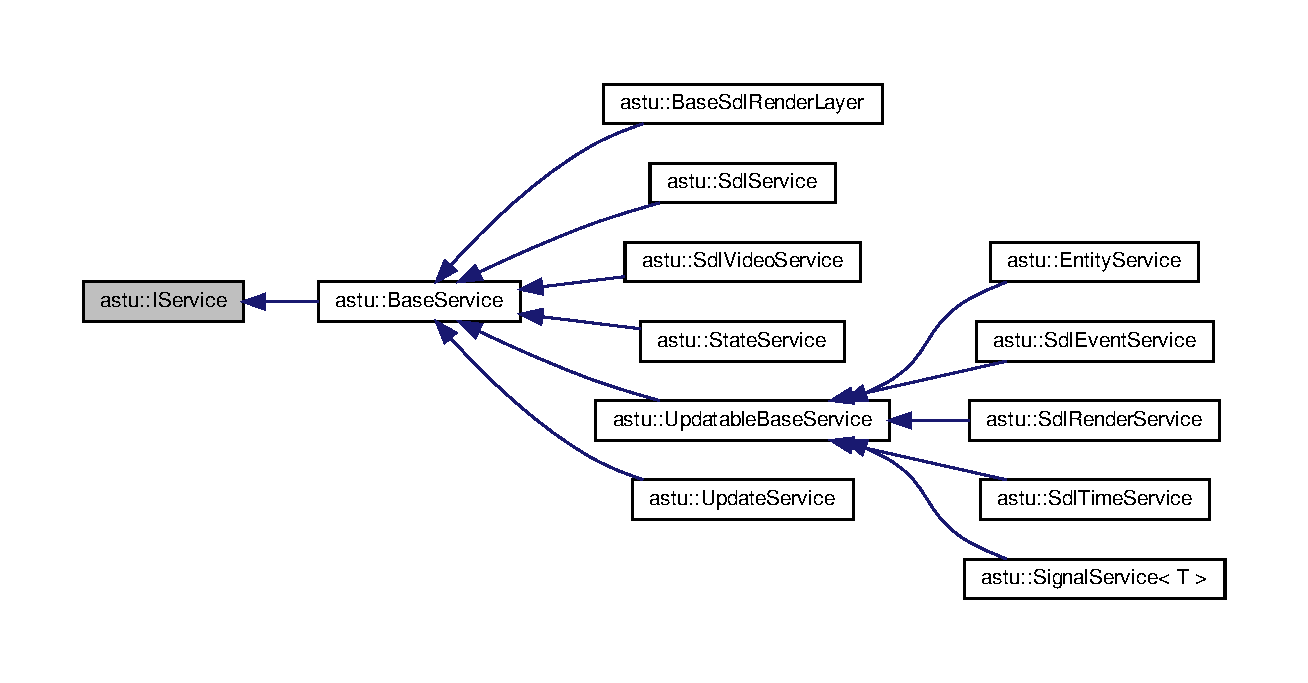
\includegraphics[width=350pt]{classastu_1_1IService__inherit__graph}
\end{center}
\end{figure}
\subsection*{Public Member Functions}
\begin{DoxyCompactItemize}
\item 
virtual \hyperlink{classastu_1_1IService_abf42fedf905da617ad881d3fd28a9d7e}{$\sim$\+I\+Service} ()
\item 
virtual const std\+::string \& \hyperlink{classastu_1_1IService_a7bfb508c07816c701ceaa72928213380}{Get\+Name} () const =0
\item 
virtual void \hyperlink{classastu_1_1IService_a7a09e485d116659f174aca9a8494fa55}{Startup} ()=0
\item 
virtual void \hyperlink{classastu_1_1IService_a67643385e7cc17c31e0b3b49672b5856}{Shutdown} ()=0
\item 
virtual bool \hyperlink{classastu_1_1IService_ab69225f6a613c8829c45d23158fba775}{Is\+Running} () const =0
\end{DoxyCompactItemize}


\subsection{Detailed Description}
Interface for services. 

\subsection{Constructor \& Destructor Documentation}
\mbox{\Hypertarget{classastu_1_1IService_abf42fedf905da617ad881d3fd28a9d7e}\label{classastu_1_1IService_abf42fedf905da617ad881d3fd28a9d7e}} 
\index{astu\+::\+I\+Service@{astu\+::\+I\+Service}!````~I\+Service@{$\sim$\+I\+Service}}
\index{````~I\+Service@{$\sim$\+I\+Service}!astu\+::\+I\+Service@{astu\+::\+I\+Service}}
\subsubsection{\texorpdfstring{$\sim$\+I\+Service()}{~IService()}}
{\footnotesize\ttfamily virtual astu\+::\+I\+Service\+::$\sim$\+I\+Service (\begin{DoxyParamCaption}{ }\end{DoxyParamCaption})\hspace{0.3cm}{\ttfamily [inline]}, {\ttfamily [virtual]}}

Virtual destructor. 

\subsection{Member Function Documentation}
\mbox{\Hypertarget{classastu_1_1IService_a7bfb508c07816c701ceaa72928213380}\label{classastu_1_1IService_a7bfb508c07816c701ceaa72928213380}} 
\index{astu\+::\+I\+Service@{astu\+::\+I\+Service}!Get\+Name@{Get\+Name}}
\index{Get\+Name@{Get\+Name}!astu\+::\+I\+Service@{astu\+::\+I\+Service}}
\subsubsection{\texorpdfstring{Get\+Name()}{GetName()}}
{\footnotesize\ttfamily virtual const std\+::string\& astu\+::\+I\+Service\+::\+Get\+Name (\begin{DoxyParamCaption}{ }\end{DoxyParamCaption}) const\hspace{0.3cm}{\ttfamily [pure virtual]}}

Returns the name of this service.

\begin{DoxyReturn}{Returns}
this service\textquotesingle{}s name 
\end{DoxyReturn}


Implemented in \hyperlink{classastu_1_1BaseService_a42eb6e0d667215ef635682d2a12e1631}{astu\+::\+Base\+Service}.

\mbox{\Hypertarget{classastu_1_1IService_ab69225f6a613c8829c45d23158fba775}\label{classastu_1_1IService_ab69225f6a613c8829c45d23158fba775}} 
\index{astu\+::\+I\+Service@{astu\+::\+I\+Service}!Is\+Running@{Is\+Running}}
\index{Is\+Running@{Is\+Running}!astu\+::\+I\+Service@{astu\+::\+I\+Service}}
\subsubsection{\texorpdfstring{Is\+Running()}{IsRunning()}}
{\footnotesize\ttfamily virtual bool astu\+::\+I\+Service\+::\+Is\+Running (\begin{DoxyParamCaption}{ }\end{DoxyParamCaption}) const\hspace{0.3cm}{\ttfamily [pure virtual]}}

Returns {\ttfamily true} if this service is running.

\begin{DoxyReturn}{Returns}
{\ttfamily true} if this service is running 
\end{DoxyReturn}


Implemented in \hyperlink{classastu_1_1BaseService_af6f4641c045343d329a0fc1ecc6a9778}{astu\+::\+Base\+Service}.

\mbox{\Hypertarget{classastu_1_1IService_a67643385e7cc17c31e0b3b49672b5856}\label{classastu_1_1IService_a67643385e7cc17c31e0b3b49672b5856}} 
\index{astu\+::\+I\+Service@{astu\+::\+I\+Service}!Shutdown@{Shutdown}}
\index{Shutdown@{Shutdown}!astu\+::\+I\+Service@{astu\+::\+I\+Service}}
\subsubsection{\texorpdfstring{Shutdown()}{Shutdown()}}
{\footnotesize\ttfamily virtual void astu\+::\+I\+Service\+::\+Shutdown (\begin{DoxyParamCaption}{ }\end{DoxyParamCaption})\hspace{0.3cm}{\ttfamily [pure virtual]}}

Stops this service.

In case this service is currently not running, calling this method has no effect. 

Implemented in \hyperlink{classastu_1_1BaseSdlRenderLayer_a786ae49f41873d498ae0d22a0f3a5349}{astu\+::\+Base\+Sdl\+Render\+Layer}, \hyperlink{classastu_1_1UpdatableBaseService_a7ad7e0201007878b6014361dd5ba82f9}{astu\+::\+Updatable\+Base\+Service}, and \hyperlink{classastu_1_1BaseService_a7095888244052db294d58738c0d187fb}{astu\+::\+Base\+Service}.

\mbox{\Hypertarget{classastu_1_1IService_a7a09e485d116659f174aca9a8494fa55}\label{classastu_1_1IService_a7a09e485d116659f174aca9a8494fa55}} 
\index{astu\+::\+I\+Service@{astu\+::\+I\+Service}!Startup@{Startup}}
\index{Startup@{Startup}!astu\+::\+I\+Service@{astu\+::\+I\+Service}}
\subsubsection{\texorpdfstring{Startup()}{Startup()}}
{\footnotesize\ttfamily virtual void astu\+::\+I\+Service\+::\+Startup (\begin{DoxyParamCaption}{ }\end{DoxyParamCaption})\hspace{0.3cm}{\ttfamily [pure virtual]}}

Starts this service.


\begin{DoxyExceptions}{Exceptions}
{\em std\+::logic\+\_\+error} & in case this service is already running \\
\hline
\end{DoxyExceptions}


Implemented in \hyperlink{classastu_1_1BaseSdlRenderLayer_a0f4fbd9bbd5613589a8f1ce39d8b6340}{astu\+::\+Base\+Sdl\+Render\+Layer}, \hyperlink{classastu_1_1UpdatableBaseService_a47e3725f717cee3cd8983f485b2a0243}{astu\+::\+Updatable\+Base\+Service}, and \hyperlink{classastu_1_1BaseService_a59dade033dcb44dd32155c526a3a58e2}{astu\+::\+Base\+Service}.



The documentation for this class was generated from the following file\+:\begin{DoxyCompactItemize}
\item 
include/Service.\+h\end{DoxyCompactItemize}

\hypertarget{classastu_1_1ISignalListener}{}\section{astu\+:\+:I\+Signal\+Listener$<$ T $>$ Class Template Reference}
\label{classastu_1_1ISignalListener}\index{astu\+::\+I\+Signal\+Listener$<$ T $>$@{astu\+::\+I\+Signal\+Listener$<$ T $>$}}


{\ttfamily \#include $<$Signal\+Service.\+h$>$}

\subsection*{Public Member Functions}
\begin{DoxyCompactItemize}
\item 
\hyperlink{classastu_1_1ISignalListener_a8656a83d9ac0775640edb97e028c3fd9}{$\sim$\+I\+Signal\+Listener} ()
\item 
virtual void \hyperlink{classastu_1_1ISignalListener_abc538ead0f63533bc60ba0f931b2a5ce}{On\+Signal} (const T \&signal)=0
\end{DoxyCompactItemize}


\subsection{Detailed Description}
\subsubsection*{template$<$typename T$>$\newline
class astu\+::\+I\+Signal\+Listener$<$ T $>$}

A template signal listeners of a certain type.

{\bfseries Example}

This example shows a signal listener which is listening to {\ttfamily int} values.

Header file\+: {\itshape My\+Listener.\+h} 
\begin{DoxyCode}
\textcolor{preprocessor}{#pragma once}

\textcolor{preprocessor}{#include <SignalService.h>}

\textcolor{keyword}{class }MyListener : \textcolor{keyword}{public} \hyperlink{classastu_1_1ISignalListener}{astu::ISignalListener}<int> \{
\textcolor{keyword}{public}:

  \textcolor{comment}{// Inheritred via ISignalListener}
  \textcolor{keyword}{virtual} \textcolor{keywordtype}{void} \hyperlink{classastu_1_1ISignalListener_abc538ead0f63533bc60ba0f931b2a5ce}{OnSignal}(\textcolor{keyword}{const} \textcolor{keywordtype}{int} & signal) \textcolor{keyword}{override};    
\};
\end{DoxyCode}


Implementation file\+: {\itshape My\+Listener.\+cpp}


\begin{DoxyCode}
\textcolor{preprocessor}{#include <iostream>}
\textcolor{preprocessor}{#include "MyListener.h"}

MyListener::void \hyperlink{classastu_1_1ISignalListener_abc538ead0f63533bc60ba0f931b2a5ce}{OnSignal}(\textcolor{keyword}{const} \textcolor{keywordtype}{int} & signal)
\{
  std::cout << \textcolor{stringliteral}{"received signal "} << signal << std::endl;
\}    
\end{DoxyCode}



\begin{DoxyTemplParams}{Template Parameters}
{\em T} & the type of signal this listeners is receiving \\
\hline
\end{DoxyTemplParams}


\subsection{Constructor \& Destructor Documentation}
\mbox{\Hypertarget{classastu_1_1ISignalListener_a8656a83d9ac0775640edb97e028c3fd9}\label{classastu_1_1ISignalListener_a8656a83d9ac0775640edb97e028c3fd9}} 
\index{astu\+::\+I\+Signal\+Listener@{astu\+::\+I\+Signal\+Listener}!````~I\+Signal\+Listener@{$\sim$\+I\+Signal\+Listener}}
\index{````~I\+Signal\+Listener@{$\sim$\+I\+Signal\+Listener}!astu\+::\+I\+Signal\+Listener@{astu\+::\+I\+Signal\+Listener}}
\subsubsection{\texorpdfstring{$\sim$\+I\+Signal\+Listener()}{~ISignalListener()}}
{\footnotesize\ttfamily template$<$typename T$>$ \\
\hyperlink{classastu_1_1ISignalListener}{astu\+::\+I\+Signal\+Listener}$<$ T $>$\+::$\sim$\hyperlink{classastu_1_1ISignalListener}{I\+Signal\+Listener} (\begin{DoxyParamCaption}{ }\end{DoxyParamCaption})\hspace{0.3cm}{\ttfamily [inline]}}

Virtual destructor. 

\subsection{Member Function Documentation}
\mbox{\Hypertarget{classastu_1_1ISignalListener_abc538ead0f63533bc60ba0f931b2a5ce}\label{classastu_1_1ISignalListener_abc538ead0f63533bc60ba0f931b2a5ce}} 
\index{astu\+::\+I\+Signal\+Listener@{astu\+::\+I\+Signal\+Listener}!On\+Signal@{On\+Signal}}
\index{On\+Signal@{On\+Signal}!astu\+::\+I\+Signal\+Listener@{astu\+::\+I\+Signal\+Listener}}
\subsubsection{\texorpdfstring{On\+Signal()}{OnSignal()}}
{\footnotesize\ttfamily template$<$typename T$>$ \\
virtual void \hyperlink{classastu_1_1ISignalListener}{astu\+::\+I\+Signal\+Listener}$<$ T $>$\+::On\+Signal (\begin{DoxyParamCaption}\item[{const T \&}]{signal }\end{DoxyParamCaption})\hspace{0.3cm}{\ttfamily [pure virtual]}}

Called when a signal should be processed by this listener.


\begin{DoxyParams}{Parameters}
{\em signal} & the signal \\
\hline
\end{DoxyParams}


The documentation for this class was generated from the following file\+:\begin{DoxyCompactItemize}
\item 
include/Signal\+Service.\+h\end{DoxyCompactItemize}

\hypertarget{classastu_1_1ITimeService}{}\section{astu\+:\+:I\+Time\+Service Class Reference}
\label{classastu_1_1ITimeService}\index{astu\+::\+I\+Time\+Service@{astu\+::\+I\+Time\+Service}}


{\ttfamily \#include $<$I\+Time\+Service.\+h$>$}



Inheritance diagram for astu\+:\+:I\+Time\+Service\+:\nopagebreak
\begin{figure}[H]
\begin{center}
\leavevmode
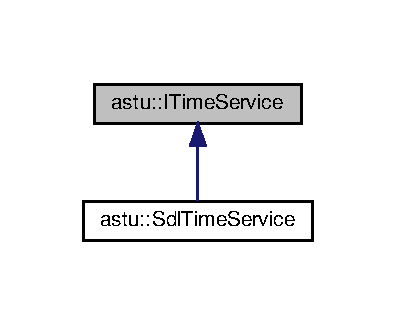
\includegraphics[width=190pt]{classastu_1_1ITimeService__inherit__graph}
\end{center}
\end{figure}
\subsection*{Public Member Functions}
\begin{DoxyCompactItemize}
\item 
\hyperlink{classastu_1_1ITimeService_a6e05093348b1c9bdc9c34ee74c85524b}{$\sim$\+I\+Time\+Service} ()
\item 
virtual double \hyperlink{classastu_1_1ITimeService_af38c6c5f4fedc705c14b01f2c61b0afc}{Get\+Elapsed\+Time} () const =0
\end{DoxyCompactItemize}


\subsection{Detailed Description}
Interface for an services which keepts track of time. 

\subsection{Constructor \& Destructor Documentation}
\mbox{\Hypertarget{classastu_1_1ITimeService_a6e05093348b1c9bdc9c34ee74c85524b}\label{classastu_1_1ITimeService_a6e05093348b1c9bdc9c34ee74c85524b}} 
\index{astu\+::\+I\+Time\+Service@{astu\+::\+I\+Time\+Service}!````~I\+Time\+Service@{$\sim$\+I\+Time\+Service}}
\index{````~I\+Time\+Service@{$\sim$\+I\+Time\+Service}!astu\+::\+I\+Time\+Service@{astu\+::\+I\+Time\+Service}}
\subsubsection{\texorpdfstring{$\sim$\+I\+Time\+Service()}{~ITimeService()}}
{\footnotesize\ttfamily astu\+::\+I\+Time\+Service\+::$\sim$\+I\+Time\+Service (\begin{DoxyParamCaption}{ }\end{DoxyParamCaption})\hspace{0.3cm}{\ttfamily [inline]}}

Virtual destructor. 

\subsection{Member Function Documentation}
\mbox{\Hypertarget{classastu_1_1ITimeService_af38c6c5f4fedc705c14b01f2c61b0afc}\label{classastu_1_1ITimeService_af38c6c5f4fedc705c14b01f2c61b0afc}} 
\index{astu\+::\+I\+Time\+Service@{astu\+::\+I\+Time\+Service}!Get\+Elapsed\+Time@{Get\+Elapsed\+Time}}
\index{Get\+Elapsed\+Time@{Get\+Elapsed\+Time}!astu\+::\+I\+Time\+Service@{astu\+::\+I\+Time\+Service}}
\subsubsection{\texorpdfstring{Get\+Elapsed\+Time()}{GetElapsedTime()}}
{\footnotesize\ttfamily virtual double astu\+::\+I\+Time\+Service\+::\+Get\+Elapsed\+Time (\begin{DoxyParamCaption}{ }\end{DoxyParamCaption}) const\hspace{0.3cm}{\ttfamily [pure virtual]}}

Returns the elapsed time since the last update.


\begin{DoxyParams}{Parameters}
{\em double} & the elapsed time in seconds \\
\hline
\end{DoxyParams}


Implemented in \hyperlink{classastu_1_1SdlTimeService_a6652d19cae14e20ec85a1808fc8e87b7}{astu\+::\+Sdl\+Time\+Service}.



The documentation for this class was generated from the following file\+:\begin{DoxyCompactItemize}
\item 
include/I\+Time\+Service.\+h\end{DoxyCompactItemize}

\hypertarget{classastu_1_1IUpdatable}{}\section{astu\+:\+:I\+Updatable Class Reference}
\label{classastu_1_1IUpdatable}\index{astu\+::\+I\+Updatable@{astu\+::\+I\+Updatable}}


{\ttfamily \#include $<$Update\+Service.\+h$>$}



Inheritance diagram for astu\+:\+:I\+Updatable\+:
\nopagebreak
\begin{figure}[H]
\begin{center}
\leavevmode
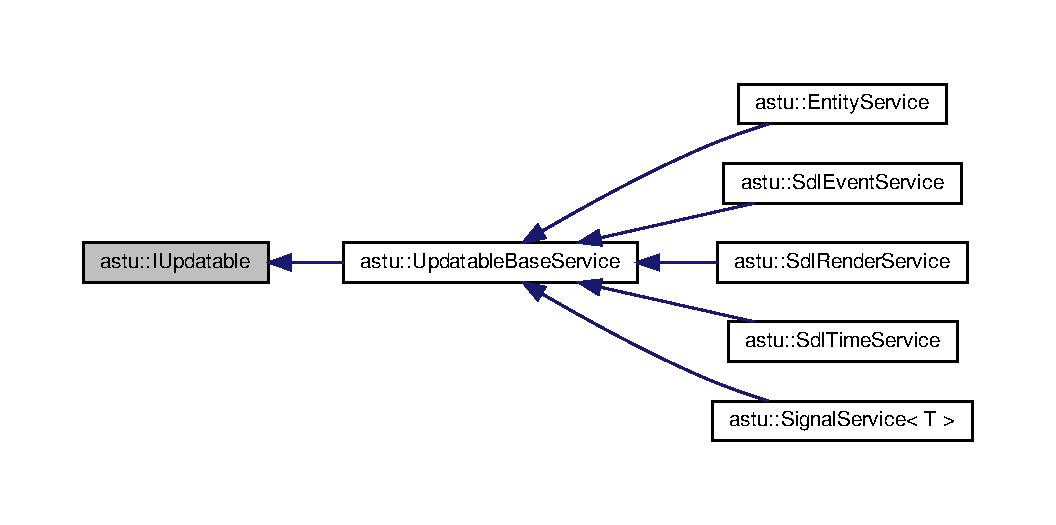
\includegraphics[width=350pt]{classastu_1_1IUpdatable__inherit__graph}
\end{center}
\end{figure}
\subsection*{Public Member Functions}
\begin{DoxyCompactItemize}
\item 
virtual \hyperlink{classastu_1_1IUpdatable_ae0ba3ec6b901ef3dd3692471222180e6}{$\sim$\+I\+Updatable} ()
\item 
virtual void \hyperlink{classastu_1_1IUpdatable_a76c7c6e2a71b725bbdbdf6808ef4743f}{On\+Update} ()=0
\end{DoxyCompactItemize}


\subsection{Detailed Description}
Interface for items that can be updated. 

\subsection{Constructor \& Destructor Documentation}
\mbox{\Hypertarget{classastu_1_1IUpdatable_ae0ba3ec6b901ef3dd3692471222180e6}\label{classastu_1_1IUpdatable_ae0ba3ec6b901ef3dd3692471222180e6}} 
\index{astu\+::\+I\+Updatable@{astu\+::\+I\+Updatable}!````~I\+Updatable@{$\sim$\+I\+Updatable}}
\index{````~I\+Updatable@{$\sim$\+I\+Updatable}!astu\+::\+I\+Updatable@{astu\+::\+I\+Updatable}}
\subsubsection{\texorpdfstring{$\sim$\+I\+Updatable()}{~IUpdatable()}}
{\footnotesize\ttfamily virtual astu\+::\+I\+Updatable\+::$\sim$\+I\+Updatable (\begin{DoxyParamCaption}{ }\end{DoxyParamCaption})\hspace{0.3cm}{\ttfamily [inline]}, {\ttfamily [virtual]}}

Virtual destructor. 

\subsection{Member Function Documentation}
\mbox{\Hypertarget{classastu_1_1IUpdatable_a76c7c6e2a71b725bbdbdf6808ef4743f}\label{classastu_1_1IUpdatable_a76c7c6e2a71b725bbdbdf6808ef4743f}} 
\index{astu\+::\+I\+Updatable@{astu\+::\+I\+Updatable}!On\+Update@{On\+Update}}
\index{On\+Update@{On\+Update}!astu\+::\+I\+Updatable@{astu\+::\+I\+Updatable}}
\subsubsection{\texorpdfstring{On\+Update()}{OnUpdate()}}
{\footnotesize\ttfamily virtual void astu\+::\+I\+Updatable\+::\+On\+Update (\begin{DoxyParamCaption}{ }\end{DoxyParamCaption})\hspace{0.3cm}{\ttfamily [pure virtual]}}

Called when an update is due. 

Implemented in \hyperlink{classastu_1_1EntityService_a70831a8dc185652c2c9056c4e3cc10e0}{astu\+::\+Entity\+Service}, \hyperlink{classastu_1_1IteratingEntitySystem_a7534ceb189ea282024bb9917cc244e94}{astu\+::\+Iterating\+Entity\+System}, \hyperlink{classastu_1_1Updatable_a925566c9770b95895c6c7294f9d51528}{astu\+::\+Updatable}, \hyperlink{classastu_1_1SdlEventService_a67090f42250433506b8bfb4254df9e50}{astu\+::\+Sdl\+Event\+Service}, \hyperlink{classastu_1_1SdlSceneGraph2D_add3a6e67064379389068659addad0920}{astu\+::\+Sdl\+Scene\+Graph2D}, \hyperlink{classastu_1_1SdlTimeService_ada8347f0f665616a2202919e71b76302}{astu\+::\+Sdl\+Time\+Service}, and \hyperlink{classastu_1_1suite2d_1_1CameraControlService_ab547e4f6103448db59d1350695bed4e8}{astu\+::suite2d\+::\+Camera\+Control\+Service}.



The documentation for this class was generated from the following file\+:\begin{DoxyCompactItemize}
\item 
include/\+Service/Update\+Service.\+h\end{DoxyCompactItemize}

\hypertarget{classastu_1_1IWindowManager}{}\section{astu\+:\+:I\+Window\+Manager Class Reference}
\label{classastu_1_1IWindowManager}\index{astu\+::\+I\+Window\+Manager@{astu\+::\+I\+Window\+Manager}}


{\ttfamily \#include $<$I\+Window\+Manager.\+h$>$}



Inheritance diagram for astu\+:\+:I\+Window\+Manager\+:\nopagebreak
\begin{figure}[H]
\begin{center}
\leavevmode
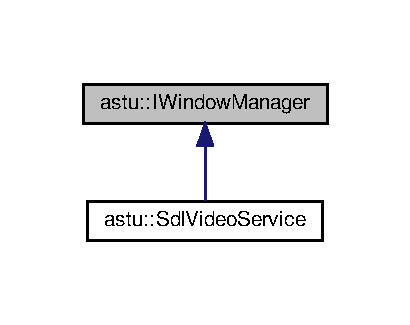
\includegraphics[width=197pt]{classastu_1_1IWindowManager__inherit__graph}
\end{center}
\end{figure}
\subsection*{Public Member Functions}
\begin{DoxyCompactItemize}
\item 
virtual \hyperlink{classastu_1_1IWindowManager_a45f1d28db89ccec4e773aaaf891d9d7b}{$\sim$\+I\+Window\+Manager} ()
\item 
virtual void \hyperlink{classastu_1_1IWindowManager_aca77eeecb7c790fa3c1d58c20dd7294f}{Set\+Size} (int width, int height)=0
\item 
virtual int \hyperlink{classastu_1_1IWindowManager_a6f818a88754bde33c3121e7413d3a554}{Get\+Width} () const =0
\item 
virtual int \hyperlink{classastu_1_1IWindowManager_a80a146779e21437e8c6ef78889389dfc}{Get\+Height} () const =0
\item 
virtual void \hyperlink{classastu_1_1IWindowManager_ae75ef0ce5ff6943712b9aa55cbfaadf8}{Set\+Title} (const std\+::string \&title)=0
\item 
virtual const std\+::string \& \hyperlink{classastu_1_1IWindowManager_aa5733f1ceda60796f6e35f5f7b79ffa9}{Get\+Title} () const =0
\end{DoxyCompactItemize}


\subsection{Detailed Description}
Interface for an services which manages application windows. 

\subsection{Constructor \& Destructor Documentation}
\mbox{\Hypertarget{classastu_1_1IWindowManager_a45f1d28db89ccec4e773aaaf891d9d7b}\label{classastu_1_1IWindowManager_a45f1d28db89ccec4e773aaaf891d9d7b}} 
\index{astu\+::\+I\+Window\+Manager@{astu\+::\+I\+Window\+Manager}!````~I\+Window\+Manager@{$\sim$\+I\+Window\+Manager}}
\index{````~I\+Window\+Manager@{$\sim$\+I\+Window\+Manager}!astu\+::\+I\+Window\+Manager@{astu\+::\+I\+Window\+Manager}}
\subsubsection{\texorpdfstring{$\sim$\+I\+Window\+Manager()}{~IWindowManager()}}
{\footnotesize\ttfamily virtual astu\+::\+I\+Window\+Manager\+::$\sim$\+I\+Window\+Manager (\begin{DoxyParamCaption}{ }\end{DoxyParamCaption})\hspace{0.3cm}{\ttfamily [inline]}, {\ttfamily [virtual]}}

Virtual destructor. 

\subsection{Member Function Documentation}
\mbox{\Hypertarget{classastu_1_1IWindowManager_a80a146779e21437e8c6ef78889389dfc}\label{classastu_1_1IWindowManager_a80a146779e21437e8c6ef78889389dfc}} 
\index{astu\+::\+I\+Window\+Manager@{astu\+::\+I\+Window\+Manager}!Get\+Height@{Get\+Height}}
\index{Get\+Height@{Get\+Height}!astu\+::\+I\+Window\+Manager@{astu\+::\+I\+Window\+Manager}}
\subsubsection{\texorpdfstring{Get\+Height()}{GetHeight()}}
{\footnotesize\ttfamily virtual int astu\+::\+I\+Window\+Manager\+::\+Get\+Height (\begin{DoxyParamCaption}{ }\end{DoxyParamCaption}) const\hspace{0.3cm}{\ttfamily [pure virtual]}}

Returns the height of the window in pixels.

\begin{DoxyReturn}{Returns}
the height in pixls 
\end{DoxyReturn}


Implemented in \hyperlink{classastu_1_1SdlVideoService_a76d0f56254c9545d4d9762349133d4af}{astu\+::\+Sdl\+Video\+Service}.

\mbox{\Hypertarget{classastu_1_1IWindowManager_aa5733f1ceda60796f6e35f5f7b79ffa9}\label{classastu_1_1IWindowManager_aa5733f1ceda60796f6e35f5f7b79ffa9}} 
\index{astu\+::\+I\+Window\+Manager@{astu\+::\+I\+Window\+Manager}!Get\+Title@{Get\+Title}}
\index{Get\+Title@{Get\+Title}!astu\+::\+I\+Window\+Manager@{astu\+::\+I\+Window\+Manager}}
\subsubsection{\texorpdfstring{Get\+Title()}{GetTitle()}}
{\footnotesize\ttfamily virtual const std\+::string\& astu\+::\+I\+Window\+Manager\+::\+Get\+Title (\begin{DoxyParamCaption}{ }\end{DoxyParamCaption}) const\hspace{0.3cm}{\ttfamily [pure virtual]}}

Returns the current window title.

\begin{DoxyReturn}{Returns}
the window title 
\end{DoxyReturn}


Implemented in \hyperlink{classastu_1_1SdlVideoService_ad6ee7f7a409960e91ddd77bbcea6432f}{astu\+::\+Sdl\+Video\+Service}.

\mbox{\Hypertarget{classastu_1_1IWindowManager_a6f818a88754bde33c3121e7413d3a554}\label{classastu_1_1IWindowManager_a6f818a88754bde33c3121e7413d3a554}} 
\index{astu\+::\+I\+Window\+Manager@{astu\+::\+I\+Window\+Manager}!Get\+Width@{Get\+Width}}
\index{Get\+Width@{Get\+Width}!astu\+::\+I\+Window\+Manager@{astu\+::\+I\+Window\+Manager}}
\subsubsection{\texorpdfstring{Get\+Width()}{GetWidth()}}
{\footnotesize\ttfamily virtual int astu\+::\+I\+Window\+Manager\+::\+Get\+Width (\begin{DoxyParamCaption}{ }\end{DoxyParamCaption}) const\hspace{0.3cm}{\ttfamily [pure virtual]}}

Returns the width of the window in pixels.

\begin{DoxyReturn}{Returns}
the width in pixls 
\end{DoxyReturn}


Implemented in \hyperlink{classastu_1_1SdlVideoService_a45c3181611e718bcfe44862baed6d520}{astu\+::\+Sdl\+Video\+Service}.

\mbox{\Hypertarget{classastu_1_1IWindowManager_aca77eeecb7c790fa3c1d58c20dd7294f}\label{classastu_1_1IWindowManager_aca77eeecb7c790fa3c1d58c20dd7294f}} 
\index{astu\+::\+I\+Window\+Manager@{astu\+::\+I\+Window\+Manager}!Set\+Size@{Set\+Size}}
\index{Set\+Size@{Set\+Size}!astu\+::\+I\+Window\+Manager@{astu\+::\+I\+Window\+Manager}}
\subsubsection{\texorpdfstring{Set\+Size()}{SetSize()}}
{\footnotesize\ttfamily virtual void astu\+::\+I\+Window\+Manager\+::\+Set\+Size (\begin{DoxyParamCaption}\item[{int}]{width,  }\item[{int}]{height }\end{DoxyParamCaption})\hspace{0.3cm}{\ttfamily [pure virtual]}}

Sets the dimension of the window.


\begin{DoxyParams}{Parameters}
{\em width} & the width of the window in pixels \\
\hline
{\em height} & the height of the window in pixels \\
\hline
\end{DoxyParams}


Implemented in \hyperlink{classastu_1_1SdlVideoService_a1c8d729ef42024bc0cc5065ecc6631c8}{astu\+::\+Sdl\+Video\+Service}.

\mbox{\Hypertarget{classastu_1_1IWindowManager_ae75ef0ce5ff6943712b9aa55cbfaadf8}\label{classastu_1_1IWindowManager_ae75ef0ce5ff6943712b9aa55cbfaadf8}} 
\index{astu\+::\+I\+Window\+Manager@{astu\+::\+I\+Window\+Manager}!Set\+Title@{Set\+Title}}
\index{Set\+Title@{Set\+Title}!astu\+::\+I\+Window\+Manager@{astu\+::\+I\+Window\+Manager}}
\subsubsection{\texorpdfstring{Set\+Title()}{SetTitle()}}
{\footnotesize\ttfamily virtual void astu\+::\+I\+Window\+Manager\+::\+Set\+Title (\begin{DoxyParamCaption}\item[{const std\+::string \&}]{title }\end{DoxyParamCaption})\hspace{0.3cm}{\ttfamily [pure virtual]}}

Sets the window title.


\begin{DoxyParams}{Parameters}
{\em title} & the title of the window \\
\hline
\end{DoxyParams}


Implemented in \hyperlink{classastu_1_1SdlVideoService_aad3c873db481dd622d6ddcea70b279af}{astu\+::\+Sdl\+Video\+Service}.



The documentation for this class was generated from the following file\+:\begin{DoxyCompactItemize}
\item 
include/I\+Window\+Manager.\+h\end{DoxyCompactItemize}

\hypertarget{classastu_1_1Mouse}{}\section{astu\+:\+:Mouse Class Reference}
\label{classastu_1_1Mouse}\index{astu\+::\+Mouse@{astu\+::\+Mouse}}


{\ttfamily \#include $<$Mouse.\+h$>$}

\subsection*{Public Member Functions}
\begin{DoxyCompactItemize}
\item 
void \hyperlink{classastu_1_1Mouse_a1f60d23fe113d85a80569a5a3539eabf}{Set\+Button} (int button, bool pressed)
\item 
bool \hyperlink{classastu_1_1Mouse_a400f6483be85ac0e4694806bdd22e25a}{Is\+Pressed} (int button) const
\end{DoxyCompactItemize}


\subsection{Detailed Description}
Provides access to mouse input.

This class is realized using the Monostate design pattern. 

\subsection{Member Function Documentation}
\mbox{\Hypertarget{classastu_1_1Mouse_a400f6483be85ac0e4694806bdd22e25a}\label{classastu_1_1Mouse_a400f6483be85ac0e4694806bdd22e25a}} 
\index{astu\+::\+Mouse@{astu\+::\+Mouse}!Is\+Pressed@{Is\+Pressed}}
\index{Is\+Pressed@{Is\+Pressed}!astu\+::\+Mouse@{astu\+::\+Mouse}}
\subsubsection{\texorpdfstring{Is\+Pressed()}{IsPressed()}}
{\footnotesize\ttfamily bool astu\+::\+Mouse\+::\+Is\+Pressed (\begin{DoxyParamCaption}\item[{int}]{button }\end{DoxyParamCaption}) const}

Returns whether a button is currently pressed.


\begin{DoxyParams}{Parameters}
{\em button} & the index of the button to query \\
\hline
\end{DoxyParams}
\begin{DoxyReturn}{Returns}
{\ttfamily true} if the button is currently pressed 
\end{DoxyReturn}
\mbox{\Hypertarget{classastu_1_1Mouse_a1f60d23fe113d85a80569a5a3539eabf}\label{classastu_1_1Mouse_a1f60d23fe113d85a80569a5a3539eabf}} 
\index{astu\+::\+Mouse@{astu\+::\+Mouse}!Set\+Button@{Set\+Button}}
\index{Set\+Button@{Set\+Button}!astu\+::\+Mouse@{astu\+::\+Mouse}}
\subsubsection{\texorpdfstring{Set\+Button()}{SetButton()}}
{\footnotesize\ttfamily void astu\+::\+Mouse\+::\+Set\+Button (\begin{DoxyParamCaption}\item[{int}]{button,  }\item[{bool}]{pressed }\end{DoxyParamCaption})}

Sets the state of a button.


\begin{DoxyParams}{Parameters}
{\em button} & the index of the button to set \\
\hline
{\em pressed} & set to {\ttfamily true} to marked the button as pressed \\
\hline
\end{DoxyParams}


The documentation for this class was generated from the following file\+:\begin{DoxyCompactItemize}
\item 
include/Mouse.\+h\end{DoxyCompactItemize}

\hypertarget{classastu_1_1MouseButtonEvent}{}\section{astu\+:\+:Mouse\+Button\+Event Class Reference}
\label{classastu_1_1MouseButtonEvent}\index{astu\+::\+Mouse\+Button\+Event@{astu\+::\+Mouse\+Button\+Event}}


{\ttfamily \#include $<$Events.\+h$>$}

\subsection*{Public Types}
\begin{DoxyCompactItemize}
\item 
\mbox{\Hypertarget{classastu_1_1MouseButtonEvent_ab01204b34a3eeeb6c92cce127feecb8b}\label{classastu_1_1MouseButtonEvent_ab01204b34a3eeeb6c92cce127feecb8b}} 
enum {\bfseries B\+U\+T\+T\+ON} \{ {\bfseries L\+E\+FT} = 1, 
{\bfseries M\+I\+D\+D\+LE} = 2, 
{\bfseries R\+I\+G\+HT} = 3
 \}
\end{DoxyCompactItemize}
\subsection*{Public Member Functions}
\begin{DoxyCompactItemize}
\item 
\mbox{\Hypertarget{classastu_1_1MouseButtonEvent_a1f1617862765f08c21e7344ab3fc0389}\label{classastu_1_1MouseButtonEvent_a1f1617862765f08c21e7344ab3fc0389}} 
{\bfseries Mouse\+Button\+Event} (int \+\_\+button=0, bool \+\_\+pressed=false)
\end{DoxyCompactItemize}
\subsection*{Public Attributes}
\begin{DoxyCompactItemize}
\item 
\mbox{\Hypertarget{classastu_1_1MouseButtonEvent_a8dfd189ee91334495030426431158d53}\label{classastu_1_1MouseButtonEvent_a8dfd189ee91334495030426431158d53}} 
int {\bfseries button}
\item 
\mbox{\Hypertarget{classastu_1_1MouseButtonEvent_ac6af684a515975ad06203d562acf0dcc}\label{classastu_1_1MouseButtonEvent_ac6af684a515975ad06203d562acf0dcc}} 
bool {\bfseries pressed}
\end{DoxyCompactItemize}


\subsection{Detailed Description}
This event represents a mouse button event.

This event is supposed to be used in combination with the \hyperlink{classastu_1_1SignalService}{Signal\+Service}. 

The documentation for this class was generated from the following file\+:\begin{DoxyCompactItemize}
\item 
include/Events.\+h\end{DoxyCompactItemize}

\hypertarget{classastu_1_1SdlEventService}{}\section{astu\+:\+:Sdl\+Event\+Service Class Reference}
\label{classastu_1_1SdlEventService}\index{astu\+::\+Sdl\+Event\+Service@{astu\+::\+Sdl\+Event\+Service}}


{\ttfamily \#include $<$Sdl\+Event\+Service.\+h$>$}



Inheritance diagram for astu\+:\+:Sdl\+Event\+Service\+:\nopagebreak
\begin{figure}[H]
\begin{center}
\leavevmode
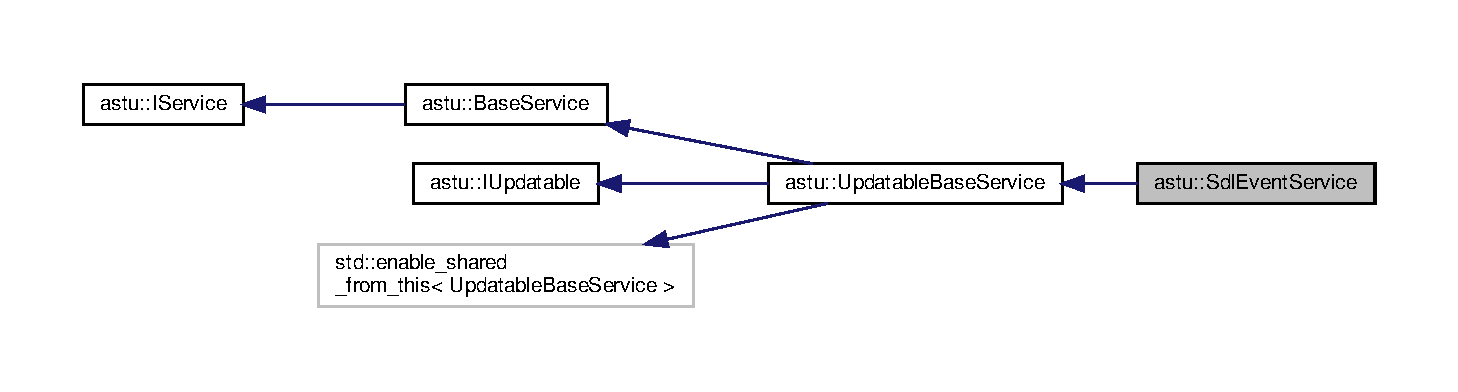
\includegraphics[width=350pt]{classastu_1_1SdlEventService__inherit__graph}
\end{center}
\end{figure}


Collaboration diagram for astu\+:\+:Sdl\+Event\+Service\+:\nopagebreak
\begin{figure}[H]
\begin{center}
\leavevmode
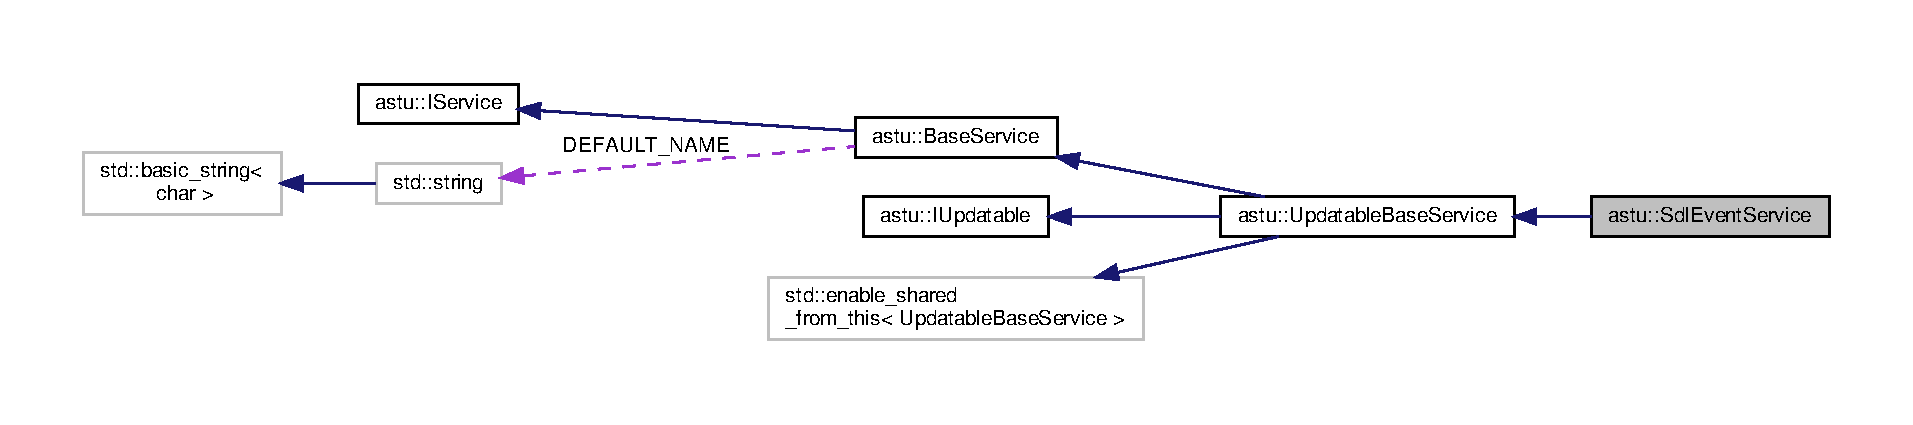
\includegraphics[width=350pt]{classastu_1_1SdlEventService__coll__graph}
\end{center}
\end{figure}
\subsection*{Public Member Functions}
\begin{DoxyCompactItemize}
\item 
\hyperlink{classastu_1_1SdlEventService_ad8da3cc63eb9810ba27a80bfeb68122d}{Sdl\+Event\+Service} (int priority=0)
\item 
\hyperlink{classastu_1_1SdlEventService_a388605cdc2ed3eb6fc70d2a020047552}{$\sim$\+Sdl\+Event\+Service} ()
\item 
bool \hyperlink{classastu_1_1SdlEventService_ac7b0eaae46bff34cc0d305a3dc3cea68}{Is\+Quit} () const
\item 
void \hyperlink{classastu_1_1SdlEventService_afe744162d9089344bfc32f6d65111ff6}{Clear\+Quit} ()
\end{DoxyCompactItemize}
\subsection*{Protected Member Functions}
\begin{DoxyCompactItemize}
\item 
virtual void \hyperlink{classastu_1_1SdlEventService_a71805a124600a23e48158daa5dc57fff}{On\+Startup} () override
\item 
virtual void \hyperlink{classastu_1_1SdlEventService_a0163bd191605b5068d93cd6c8f26da0c}{On\+Shutdown} () override
\item 
virtual void \hyperlink{classastu_1_1SdlEventService_a67090f42250433506b8bfb4254df9e50}{On\+Update} () override
\end{DoxyCompactItemize}
\subsection*{Additional Inherited Members}


\subsection{Detailed Description}
Initializes the S\+DL event submodule.

This service processes the S\+DL event queue and distributes the events through the various abstractions layers (input, window-\/handling, etc.). 

\subsection{Constructor \& Destructor Documentation}
\mbox{\Hypertarget{classastu_1_1SdlEventService_ad8da3cc63eb9810ba27a80bfeb68122d}\label{classastu_1_1SdlEventService_ad8da3cc63eb9810ba27a80bfeb68122d}} 
\index{astu\+::\+Sdl\+Event\+Service@{astu\+::\+Sdl\+Event\+Service}!Sdl\+Event\+Service@{Sdl\+Event\+Service}}
\index{Sdl\+Event\+Service@{Sdl\+Event\+Service}!astu\+::\+Sdl\+Event\+Service@{astu\+::\+Sdl\+Event\+Service}}
\subsubsection{\texorpdfstring{Sdl\+Event\+Service()}{SdlEventService()}}
{\footnotesize\ttfamily astu\+::\+Sdl\+Event\+Service\+::\+Sdl\+Event\+Service (\begin{DoxyParamCaption}\item[{int}]{priority = {\ttfamily 0} }\end{DoxyParamCaption})}

Constructor.


\begin{DoxyParams}{Parameters}
{\em priority} & the priority used to update this service \\
\hline
\end{DoxyParams}
\mbox{\Hypertarget{classastu_1_1SdlEventService_a388605cdc2ed3eb6fc70d2a020047552}\label{classastu_1_1SdlEventService_a388605cdc2ed3eb6fc70d2a020047552}} 
\index{astu\+::\+Sdl\+Event\+Service@{astu\+::\+Sdl\+Event\+Service}!````~Sdl\+Event\+Service@{$\sim$\+Sdl\+Event\+Service}}
\index{````~Sdl\+Event\+Service@{$\sim$\+Sdl\+Event\+Service}!astu\+::\+Sdl\+Event\+Service@{astu\+::\+Sdl\+Event\+Service}}
\subsubsection{\texorpdfstring{$\sim$\+Sdl\+Event\+Service()}{~SdlEventService()}}
{\footnotesize\ttfamily astu\+::\+Sdl\+Event\+Service\+::$\sim$\+Sdl\+Event\+Service (\begin{DoxyParamCaption}{ }\end{DoxyParamCaption})\hspace{0.3cm}{\ttfamily [inline]}}

Virtual destructor. 

\subsection{Member Function Documentation}
\mbox{\Hypertarget{classastu_1_1SdlEventService_afe744162d9089344bfc32f6d65111ff6}\label{classastu_1_1SdlEventService_afe744162d9089344bfc32f6d65111ff6}} 
\index{astu\+::\+Sdl\+Event\+Service@{astu\+::\+Sdl\+Event\+Service}!Clear\+Quit@{Clear\+Quit}}
\index{Clear\+Quit@{Clear\+Quit}!astu\+::\+Sdl\+Event\+Service@{astu\+::\+Sdl\+Event\+Service}}
\subsubsection{\texorpdfstring{Clear\+Quit()}{ClearQuit()}}
{\footnotesize\ttfamily void astu\+::\+Sdl\+Event\+Service\+::\+Clear\+Quit (\begin{DoxyParamCaption}{ }\end{DoxyParamCaption})}

Clears the quit-\/signal if set. \mbox{\Hypertarget{classastu_1_1SdlEventService_ac7b0eaae46bff34cc0d305a3dc3cea68}\label{classastu_1_1SdlEventService_ac7b0eaae46bff34cc0d305a3dc3cea68}} 
\index{astu\+::\+Sdl\+Event\+Service@{astu\+::\+Sdl\+Event\+Service}!Is\+Quit@{Is\+Quit}}
\index{Is\+Quit@{Is\+Quit}!astu\+::\+Sdl\+Event\+Service@{astu\+::\+Sdl\+Event\+Service}}
\subsubsection{\texorpdfstring{Is\+Quit()}{IsQuit()}}
{\footnotesize\ttfamily bool astu\+::\+Sdl\+Event\+Service\+::\+Is\+Quit (\begin{DoxyParamCaption}{ }\end{DoxyParamCaption}) const}

Return whether a quit-\/signal has been detected.

\begin{DoxyReturn}{Returns}
{\ttfamily true} if a quit-\/signal has been detected 
\end{DoxyReturn}
\mbox{\Hypertarget{classastu_1_1SdlEventService_a0163bd191605b5068d93cd6c8f26da0c}\label{classastu_1_1SdlEventService_a0163bd191605b5068d93cd6c8f26da0c}} 
\index{astu\+::\+Sdl\+Event\+Service@{astu\+::\+Sdl\+Event\+Service}!On\+Shutdown@{On\+Shutdown}}
\index{On\+Shutdown@{On\+Shutdown}!astu\+::\+Sdl\+Event\+Service@{astu\+::\+Sdl\+Event\+Service}}
\subsubsection{\texorpdfstring{On\+Shutdown()}{OnShutdown()}}
{\footnotesize\ttfamily virtual void astu\+::\+Sdl\+Event\+Service\+::\+On\+Shutdown (\begin{DoxyParamCaption}{ }\end{DoxyParamCaption})\hspace{0.3cm}{\ttfamily [override]}, {\ttfamily [protected]}, {\ttfamily [virtual]}}

Called by this base class on shutdown.

Derived classes should override this method rather than {\ttfamily \hyperlink{classastu_1_1UpdatableBaseService_a7ad7e0201007878b6014361dd5ba82f9}{Shutdown()}}. The {\ttfamily \hyperlink{classastu_1_1UpdatableBaseService_a7ad7e0201007878b6014361dd5ba82f9}{Shutdown()}} method is maintaining the running-\/state of this service. 

Reimplemented from \hyperlink{classastu_1_1BaseService_aeb5003f7c5efe5412725ac4c66942d03}{astu\+::\+Base\+Service}.

\mbox{\Hypertarget{classastu_1_1SdlEventService_a71805a124600a23e48158daa5dc57fff}\label{classastu_1_1SdlEventService_a71805a124600a23e48158daa5dc57fff}} 
\index{astu\+::\+Sdl\+Event\+Service@{astu\+::\+Sdl\+Event\+Service}!On\+Startup@{On\+Startup}}
\index{On\+Startup@{On\+Startup}!astu\+::\+Sdl\+Event\+Service@{astu\+::\+Sdl\+Event\+Service}}
\subsubsection{\texorpdfstring{On\+Startup()}{OnStartup()}}
{\footnotesize\ttfamily virtual void astu\+::\+Sdl\+Event\+Service\+::\+On\+Startup (\begin{DoxyParamCaption}{ }\end{DoxyParamCaption})\hspace{0.3cm}{\ttfamily [override]}, {\ttfamily [protected]}, {\ttfamily [virtual]}}

Called by this base class on startup.

Derived classes should override this method rather than {\ttfamily \hyperlink{classastu_1_1UpdatableBaseService_a47e3725f717cee3cd8983f485b2a0243}{Startup()}}. The {\ttfamily \hyperlink{classastu_1_1UpdatableBaseService_a47e3725f717cee3cd8983f485b2a0243}{Startup()}} method is maintaining the running-\/state of this service. 

Reimplemented from \hyperlink{classastu_1_1BaseService_ac8710cd2d6dcc990db65e7c8ccfbc5ff}{astu\+::\+Base\+Service}.

\mbox{\Hypertarget{classastu_1_1SdlEventService_a67090f42250433506b8bfb4254df9e50}\label{classastu_1_1SdlEventService_a67090f42250433506b8bfb4254df9e50}} 
\index{astu\+::\+Sdl\+Event\+Service@{astu\+::\+Sdl\+Event\+Service}!On\+Update@{On\+Update}}
\index{On\+Update@{On\+Update}!astu\+::\+Sdl\+Event\+Service@{astu\+::\+Sdl\+Event\+Service}}
\subsubsection{\texorpdfstring{On\+Update()}{OnUpdate()}}
{\footnotesize\ttfamily virtual void astu\+::\+Sdl\+Event\+Service\+::\+On\+Update (\begin{DoxyParamCaption}{ }\end{DoxyParamCaption})\hspace{0.3cm}{\ttfamily [override]}, {\ttfamily [protected]}, {\ttfamily [virtual]}}

Called when this updatable gets updated. 

Implements \hyperlink{classastu_1_1IUpdatable_a76c7c6e2a71b725bbdbdf6808ef4743f}{astu\+::\+I\+Updatable}.



The documentation for this class was generated from the following file\+:\begin{DoxyCompactItemize}
\item 
include/Sdl\+Event\+Service.\+h\end{DoxyCompactItemize}

\hypertarget{classastu_1_1SdlRenderService}{}\section{astu\+:\+:Sdl\+Render\+Service Class Reference}
\label{classastu_1_1SdlRenderService}\index{astu\+::\+Sdl\+Render\+Service@{astu\+::\+Sdl\+Render\+Service}}


{\ttfamily \#include $<$Sdl\+Render\+Service.\+h$>$}



Inheritance diagram for astu\+:\+:Sdl\+Render\+Service\+:\nopagebreak
\begin{figure}[H]
\begin{center}
\leavevmode
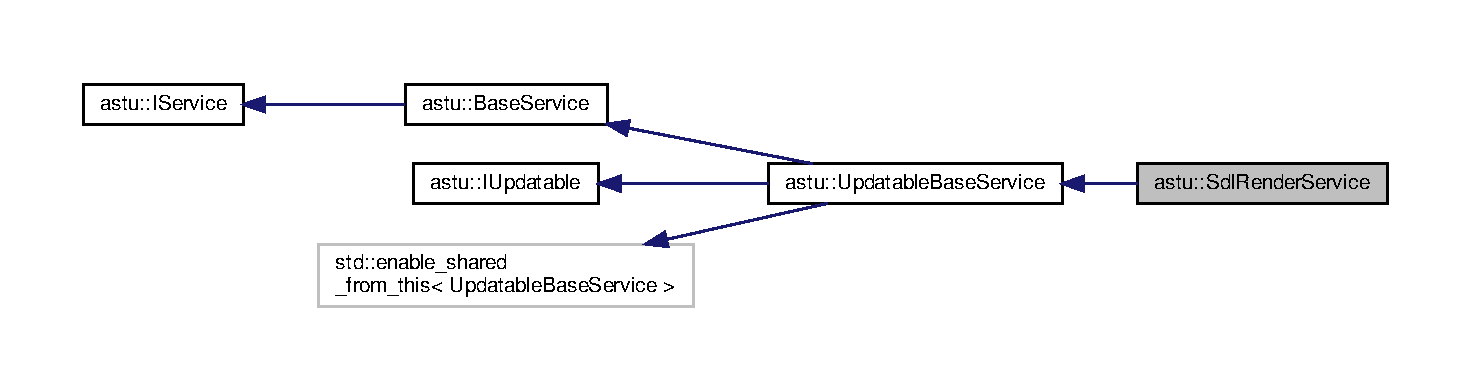
\includegraphics[width=350pt]{classastu_1_1SdlRenderService__inherit__graph}
\end{center}
\end{figure}


Collaboration diagram for astu\+:\+:Sdl\+Render\+Service\+:\nopagebreak
\begin{figure}[H]
\begin{center}
\leavevmode
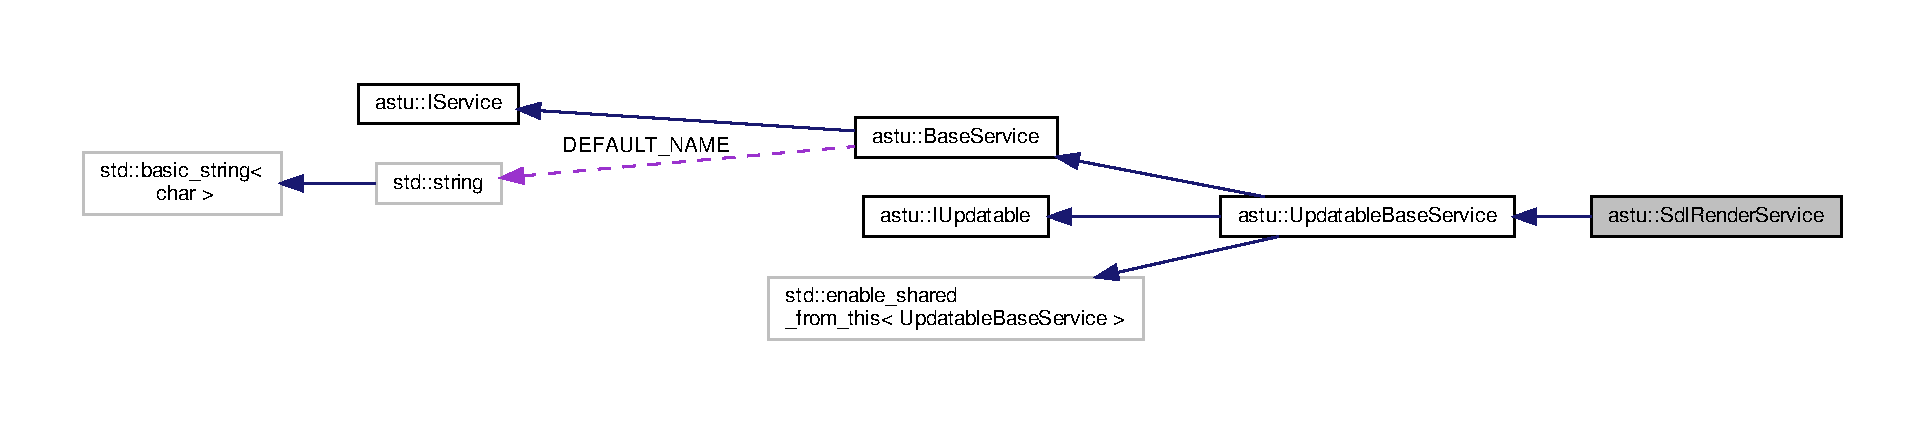
\includegraphics[width=350pt]{classastu_1_1SdlRenderService__coll__graph}
\end{center}
\end{figure}
\subsection*{Public Member Functions}
\begin{DoxyCompactItemize}
\item 
\hyperlink{classastu_1_1SdlRenderService_a8669793d9701f979c90cd802575a2645}{Sdl\+Render\+Service} (int priority=0)
\item 
virtual \hyperlink{classastu_1_1SdlRenderService_a0ec8c27982cfa6ace6b28e50fba78f2a}{$\sim$\+Sdl\+Render\+Service} ()
\item 
void \hyperlink{classastu_1_1SdlRenderService_af025dba6e6ada1f09badaa6de75292d1}{Add\+Layer} (std\+::shared\+\_\+ptr$<$ \hyperlink{classastu_1_1ISdlRenderLayer}{I\+Sdl\+Render\+Layer} $>$ layer)
\item 
void \hyperlink{classastu_1_1SdlRenderService_a88ffe81ca6348b12b0185310932bd4ee}{Remove\+Layer} (std\+::shared\+\_\+ptr$<$ \hyperlink{classastu_1_1ISdlRenderLayer}{I\+Sdl\+Render\+Layer} $>$ layer)
\item 
bool \hyperlink{classastu_1_1SdlRenderService_a45016463f301b52b1ffacfa976eb9849}{Has\+Layer} (std\+::shared\+\_\+ptr$<$ \hyperlink{classastu_1_1ISdlRenderLayer}{I\+Sdl\+Render\+Layer} $>$ layer)
\end{DoxyCompactItemize}
\subsection*{Protected Member Functions}
\begin{DoxyCompactItemize}
\item 
virtual void \hyperlink{classastu_1_1SdlRenderService_a38abd541e8075e5e4eb702ca99c9b0a5}{On\+Startup} () override
\item 
virtual void \hyperlink{classastu_1_1SdlRenderService_a4f21478ca10de11d260792c3ccd79eef}{On\+Shutdown} () override
\item 
virtual void \hyperlink{classastu_1_1SdlRenderService_af109517e98ab8bce1e625122a441fb75}{On\+Update} () override
\end{DoxyCompactItemize}
\subsection*{Additional Inherited Members}


\subsection{Detailed Description}
Initializes and maintains an S\+DL renderer.

This service has a depencendy to \hyperlink{classastu_1_1SdlVideoService}{Sdl\+Video\+Service} because creating an S\+DL renderer requires access to the S\+DL window. 

\subsection{Constructor \& Destructor Documentation}
\mbox{\Hypertarget{classastu_1_1SdlRenderService_a8669793d9701f979c90cd802575a2645}\label{classastu_1_1SdlRenderService_a8669793d9701f979c90cd802575a2645}} 
\index{astu\+::\+Sdl\+Render\+Service@{astu\+::\+Sdl\+Render\+Service}!Sdl\+Render\+Service@{Sdl\+Render\+Service}}
\index{Sdl\+Render\+Service@{Sdl\+Render\+Service}!astu\+::\+Sdl\+Render\+Service@{astu\+::\+Sdl\+Render\+Service}}
\subsubsection{\texorpdfstring{Sdl\+Render\+Service()}{SdlRenderService()}}
{\footnotesize\ttfamily astu\+::\+Sdl\+Render\+Service\+::\+Sdl\+Render\+Service (\begin{DoxyParamCaption}\item[{int}]{priority = {\ttfamily 0} }\end{DoxyParamCaption})}

Constructor.


\begin{DoxyParams}{Parameters}
{\em priority} & the priority used to update this service \\
\hline
\end{DoxyParams}
\mbox{\Hypertarget{classastu_1_1SdlRenderService_a0ec8c27982cfa6ace6b28e50fba78f2a}\label{classastu_1_1SdlRenderService_a0ec8c27982cfa6ace6b28e50fba78f2a}} 
\index{astu\+::\+Sdl\+Render\+Service@{astu\+::\+Sdl\+Render\+Service}!````~Sdl\+Render\+Service@{$\sim$\+Sdl\+Render\+Service}}
\index{````~Sdl\+Render\+Service@{$\sim$\+Sdl\+Render\+Service}!astu\+::\+Sdl\+Render\+Service@{astu\+::\+Sdl\+Render\+Service}}
\subsubsection{\texorpdfstring{$\sim$\+Sdl\+Render\+Service()}{~SdlRenderService()}}
{\footnotesize\ttfamily virtual astu\+::\+Sdl\+Render\+Service\+::$\sim$\+Sdl\+Render\+Service (\begin{DoxyParamCaption}{ }\end{DoxyParamCaption})\hspace{0.3cm}{\ttfamily [inline]}, {\ttfamily [virtual]}}

Virtual destructor. 

\subsection{Member Function Documentation}
\mbox{\Hypertarget{classastu_1_1SdlRenderService_af025dba6e6ada1f09badaa6de75292d1}\label{classastu_1_1SdlRenderService_af025dba6e6ada1f09badaa6de75292d1}} 
\index{astu\+::\+Sdl\+Render\+Service@{astu\+::\+Sdl\+Render\+Service}!Add\+Layer@{Add\+Layer}}
\index{Add\+Layer@{Add\+Layer}!astu\+::\+Sdl\+Render\+Service@{astu\+::\+Sdl\+Render\+Service}}
\subsubsection{\texorpdfstring{Add\+Layer()}{AddLayer()}}
{\footnotesize\ttfamily void astu\+::\+Sdl\+Render\+Service\+::\+Add\+Layer (\begin{DoxyParamCaption}\item[{std\+::shared\+\_\+ptr$<$ \hyperlink{classastu_1_1ISdlRenderLayer}{I\+Sdl\+Render\+Layer} $>$}]{layer }\end{DoxyParamCaption})}

Adds a render layer to this service.


\begin{DoxyParams}{Parameters}
{\em layer} & the render layer to add \\
\hline
\end{DoxyParams}
\mbox{\Hypertarget{classastu_1_1SdlRenderService_a45016463f301b52b1ffacfa976eb9849}\label{classastu_1_1SdlRenderService_a45016463f301b52b1ffacfa976eb9849}} 
\index{astu\+::\+Sdl\+Render\+Service@{astu\+::\+Sdl\+Render\+Service}!Has\+Layer@{Has\+Layer}}
\index{Has\+Layer@{Has\+Layer}!astu\+::\+Sdl\+Render\+Service@{astu\+::\+Sdl\+Render\+Service}}
\subsubsection{\texorpdfstring{Has\+Layer()}{HasLayer()}}
{\footnotesize\ttfamily bool astu\+::\+Sdl\+Render\+Service\+::\+Has\+Layer (\begin{DoxyParamCaption}\item[{std\+::shared\+\_\+ptr$<$ \hyperlink{classastu_1_1ISdlRenderLayer}{I\+Sdl\+Render\+Layer} $>$}]{layer }\end{DoxyParamCaption})}

Tests whether a render layer has already been added.


\begin{DoxyParams}{Parameters}
{\em layer} & the render to test \\
\hline
\end{DoxyParams}
\begin{DoxyReturn}{Returns}
{\ttfamily true} if the layer has already been added 
\end{DoxyReturn}
\mbox{\Hypertarget{classastu_1_1SdlRenderService_a4f21478ca10de11d260792c3ccd79eef}\label{classastu_1_1SdlRenderService_a4f21478ca10de11d260792c3ccd79eef}} 
\index{astu\+::\+Sdl\+Render\+Service@{astu\+::\+Sdl\+Render\+Service}!On\+Shutdown@{On\+Shutdown}}
\index{On\+Shutdown@{On\+Shutdown}!astu\+::\+Sdl\+Render\+Service@{astu\+::\+Sdl\+Render\+Service}}
\subsubsection{\texorpdfstring{On\+Shutdown()}{OnShutdown()}}
{\footnotesize\ttfamily virtual void astu\+::\+Sdl\+Render\+Service\+::\+On\+Shutdown (\begin{DoxyParamCaption}{ }\end{DoxyParamCaption})\hspace{0.3cm}{\ttfamily [override]}, {\ttfamily [protected]}, {\ttfamily [virtual]}}

Called by this base class on shutdown.

Derived classes should override this method rather than {\ttfamily \hyperlink{classastu_1_1UpdatableBaseService_a7ad7e0201007878b6014361dd5ba82f9}{Shutdown()}}. The {\ttfamily \hyperlink{classastu_1_1UpdatableBaseService_a7ad7e0201007878b6014361dd5ba82f9}{Shutdown()}} method is maintaining the running-\/state of this service. 

Reimplemented from \hyperlink{classastu_1_1BaseService_aeb5003f7c5efe5412725ac4c66942d03}{astu\+::\+Base\+Service}.

\mbox{\Hypertarget{classastu_1_1SdlRenderService_a38abd541e8075e5e4eb702ca99c9b0a5}\label{classastu_1_1SdlRenderService_a38abd541e8075e5e4eb702ca99c9b0a5}} 
\index{astu\+::\+Sdl\+Render\+Service@{astu\+::\+Sdl\+Render\+Service}!On\+Startup@{On\+Startup}}
\index{On\+Startup@{On\+Startup}!astu\+::\+Sdl\+Render\+Service@{astu\+::\+Sdl\+Render\+Service}}
\subsubsection{\texorpdfstring{On\+Startup()}{OnStartup()}}
{\footnotesize\ttfamily virtual void astu\+::\+Sdl\+Render\+Service\+::\+On\+Startup (\begin{DoxyParamCaption}{ }\end{DoxyParamCaption})\hspace{0.3cm}{\ttfamily [override]}, {\ttfamily [protected]}, {\ttfamily [virtual]}}

Called by this base class on startup.

Derived classes should override this method rather than {\ttfamily \hyperlink{classastu_1_1UpdatableBaseService_a47e3725f717cee3cd8983f485b2a0243}{Startup()}}. The {\ttfamily \hyperlink{classastu_1_1UpdatableBaseService_a47e3725f717cee3cd8983f485b2a0243}{Startup()}} method is maintaining the running-\/state of this service. 

Reimplemented from \hyperlink{classastu_1_1BaseService_ac8710cd2d6dcc990db65e7c8ccfbc5ff}{astu\+::\+Base\+Service}.

\mbox{\Hypertarget{classastu_1_1SdlRenderService_af109517e98ab8bce1e625122a441fb75}\label{classastu_1_1SdlRenderService_af109517e98ab8bce1e625122a441fb75}} 
\index{astu\+::\+Sdl\+Render\+Service@{astu\+::\+Sdl\+Render\+Service}!On\+Update@{On\+Update}}
\index{On\+Update@{On\+Update}!astu\+::\+Sdl\+Render\+Service@{astu\+::\+Sdl\+Render\+Service}}
\subsubsection{\texorpdfstring{On\+Update()}{OnUpdate()}}
{\footnotesize\ttfamily virtual void astu\+::\+Sdl\+Render\+Service\+::\+On\+Update (\begin{DoxyParamCaption}{ }\end{DoxyParamCaption})\hspace{0.3cm}{\ttfamily [override]}, {\ttfamily [protected]}, {\ttfamily [virtual]}}

Called when this updatable gets updated. 

Implements \hyperlink{classastu_1_1IUpdatable_a76c7c6e2a71b725bbdbdf6808ef4743f}{astu\+::\+I\+Updatable}.

\mbox{\Hypertarget{classastu_1_1SdlRenderService_a88ffe81ca6348b12b0185310932bd4ee}\label{classastu_1_1SdlRenderService_a88ffe81ca6348b12b0185310932bd4ee}} 
\index{astu\+::\+Sdl\+Render\+Service@{astu\+::\+Sdl\+Render\+Service}!Remove\+Layer@{Remove\+Layer}}
\index{Remove\+Layer@{Remove\+Layer}!astu\+::\+Sdl\+Render\+Service@{astu\+::\+Sdl\+Render\+Service}}
\subsubsection{\texorpdfstring{Remove\+Layer()}{RemoveLayer()}}
{\footnotesize\ttfamily void astu\+::\+Sdl\+Render\+Service\+::\+Remove\+Layer (\begin{DoxyParamCaption}\item[{std\+::shared\+\_\+ptr$<$ \hyperlink{classastu_1_1ISdlRenderLayer}{I\+Sdl\+Render\+Layer} $>$}]{layer }\end{DoxyParamCaption})}

Removes a render layer from this service.


\begin{DoxyParams}{Parameters}
{\em layer} & the render layer to remove \\
\hline
\end{DoxyParams}


The documentation for this class was generated from the following file\+:\begin{DoxyCompactItemize}
\item 
include/Sdl\+Render\+Service.\+h\end{DoxyCompactItemize}

\hypertarget{classastu_1_1SdlService}{}\section{astu\+:\+:Sdl\+Service Class Reference}
\label{classastu_1_1SdlService}\index{astu\+::\+Sdl\+Service@{astu\+::\+Sdl\+Service}}


{\ttfamily \#include $<$Sdl\+Service.\+h$>$}



Inheritance diagram for astu\+:\+:Sdl\+Service\+:\nopagebreak
\begin{figure}[H]
\begin{center}
\leavevmode
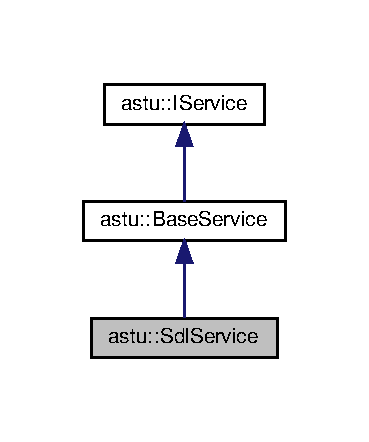
\includegraphics[width=177pt]{classastu_1_1SdlService__inherit__graph}
\end{center}
\end{figure}


Collaboration diagram for astu\+:\+:Sdl\+Service\+:\nopagebreak
\begin{figure}[H]
\begin{center}
\leavevmode
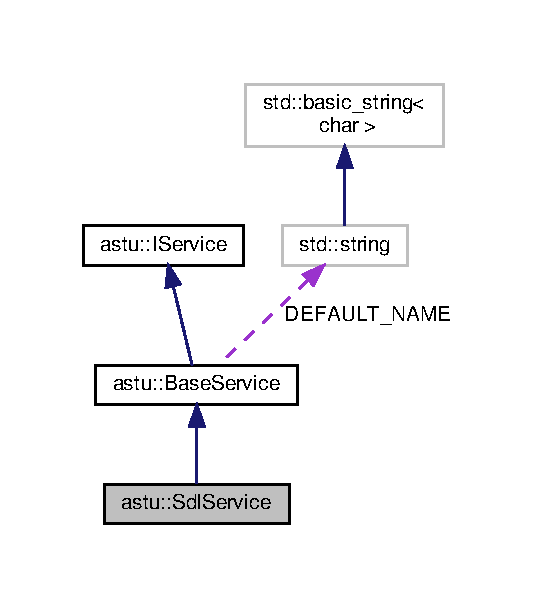
\includegraphics[width=258pt]{classastu_1_1SdlService__coll__graph}
\end{center}
\end{figure}
\subsection*{Public Member Functions}
\begin{DoxyCompactItemize}
\item 
\hyperlink{classastu_1_1SdlService_a10f72400e58e333f831d9a05d83b2d5b}{Sdl\+Service} (bool debug=false)
\end{DoxyCompactItemize}
\subsection*{Protected Member Functions}
\begin{DoxyCompactItemize}
\item 
virtual void \hyperlink{classastu_1_1SdlService_a2fcb46537de794ab6e4f5e043b26ff60}{On\+Startup} () override
\item 
virtual void \hyperlink{classastu_1_1SdlService_a20d53237efd1c717d773a8ff121b093b}{On\+Shutdown} () override
\end{DoxyCompactItemize}
\subsection*{Additional Inherited Members}


\subsection{Detailed Description}
Provides core functionality for S\+DL. 

\subsection{Constructor \& Destructor Documentation}
\mbox{\Hypertarget{classastu_1_1SdlService_a10f72400e58e333f831d9a05d83b2d5b}\label{classastu_1_1SdlService_a10f72400e58e333f831d9a05d83b2d5b}} 
\index{astu\+::\+Sdl\+Service@{astu\+::\+Sdl\+Service}!Sdl\+Service@{Sdl\+Service}}
\index{Sdl\+Service@{Sdl\+Service}!astu\+::\+Sdl\+Service@{astu\+::\+Sdl\+Service}}
\subsubsection{\texorpdfstring{Sdl\+Service()}{SdlService()}}
{\footnotesize\ttfamily astu\+::\+Sdl\+Service\+::\+Sdl\+Service (\begin{DoxyParamCaption}\item[{bool}]{debug = {\ttfamily false} }\end{DoxyParamCaption})}

Constructor. 

\subsection{Member Function Documentation}
\mbox{\Hypertarget{classastu_1_1SdlService_a20d53237efd1c717d773a8ff121b093b}\label{classastu_1_1SdlService_a20d53237efd1c717d773a8ff121b093b}} 
\index{astu\+::\+Sdl\+Service@{astu\+::\+Sdl\+Service}!On\+Shutdown@{On\+Shutdown}}
\index{On\+Shutdown@{On\+Shutdown}!astu\+::\+Sdl\+Service@{astu\+::\+Sdl\+Service}}
\subsubsection{\texorpdfstring{On\+Shutdown()}{OnShutdown()}}
{\footnotesize\ttfamily virtual void astu\+::\+Sdl\+Service\+::\+On\+Shutdown (\begin{DoxyParamCaption}{ }\end{DoxyParamCaption})\hspace{0.3cm}{\ttfamily [override]}, {\ttfamily [protected]}, {\ttfamily [virtual]}}

Called by this base class on shutdown.

Derived classes should override this method rather than {\ttfamily \hyperlink{classastu_1_1BaseService_a7095888244052db294d58738c0d187fb}{Shutdown()}}. The {\ttfamily \hyperlink{classastu_1_1BaseService_a7095888244052db294d58738c0d187fb}{Shutdown()}} method is maintaining the running-\/state of this service. 

Reimplemented from \hyperlink{classastu_1_1BaseService_aeb5003f7c5efe5412725ac4c66942d03}{astu\+::\+Base\+Service}.

\mbox{\Hypertarget{classastu_1_1SdlService_a2fcb46537de794ab6e4f5e043b26ff60}\label{classastu_1_1SdlService_a2fcb46537de794ab6e4f5e043b26ff60}} 
\index{astu\+::\+Sdl\+Service@{astu\+::\+Sdl\+Service}!On\+Startup@{On\+Startup}}
\index{On\+Startup@{On\+Startup}!astu\+::\+Sdl\+Service@{astu\+::\+Sdl\+Service}}
\subsubsection{\texorpdfstring{On\+Startup()}{OnStartup()}}
{\footnotesize\ttfamily virtual void astu\+::\+Sdl\+Service\+::\+On\+Startup (\begin{DoxyParamCaption}{ }\end{DoxyParamCaption})\hspace{0.3cm}{\ttfamily [override]}, {\ttfamily [protected]}, {\ttfamily [virtual]}}

Called by this base class on startup.

Derived classes should override this method rather than {\ttfamily \hyperlink{classastu_1_1BaseService_a59dade033dcb44dd32155c526a3a58e2}{Startup()}}. The {\ttfamily \hyperlink{classastu_1_1BaseService_a59dade033dcb44dd32155c526a3a58e2}{Startup()}} method is maintaining the running-\/state of this service. 

Reimplemented from \hyperlink{classastu_1_1BaseService_ac8710cd2d6dcc990db65e7c8ccfbc5ff}{astu\+::\+Base\+Service}.



The documentation for this class was generated from the following file\+:\begin{DoxyCompactItemize}
\item 
include/Sdl\+Service.\+h\end{DoxyCompactItemize}

\hypertarget{classastu_1_1SdlTimeService}{}\section{astu\+:\+:Sdl\+Time\+Service Class Reference}
\label{classastu_1_1SdlTimeService}\index{astu\+::\+Sdl\+Time\+Service@{astu\+::\+Sdl\+Time\+Service}}


{\ttfamily \#include $<$Sdl\+Time\+Service.\+h$>$}



Inheritance diagram for astu\+:\+:Sdl\+Time\+Service\+:\nopagebreak
\begin{figure}[H]
\begin{center}
\leavevmode
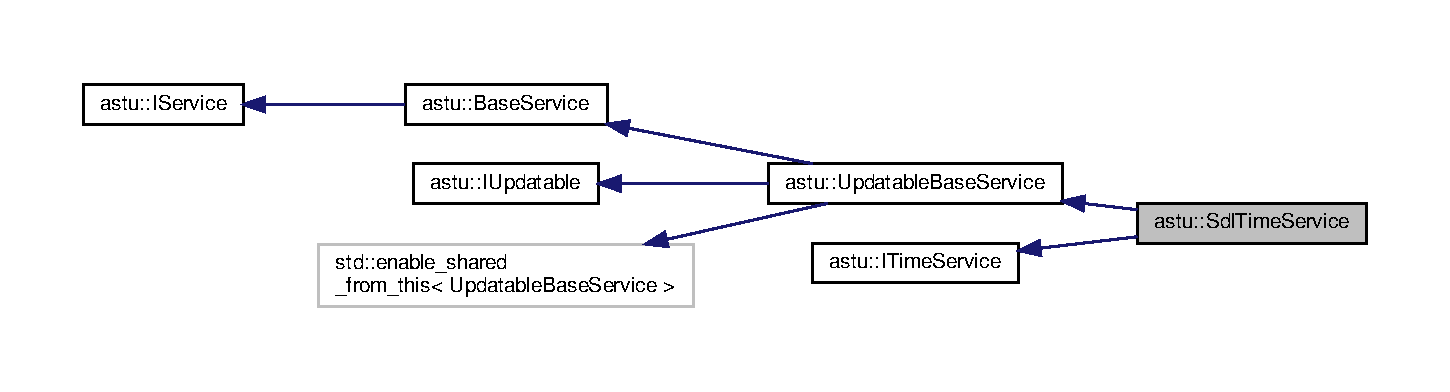
\includegraphics[width=350pt]{classastu_1_1SdlTimeService__inherit__graph}
\end{center}
\end{figure}


Collaboration diagram for astu\+:\+:Sdl\+Time\+Service\+:\nopagebreak
\begin{figure}[H]
\begin{center}
\leavevmode
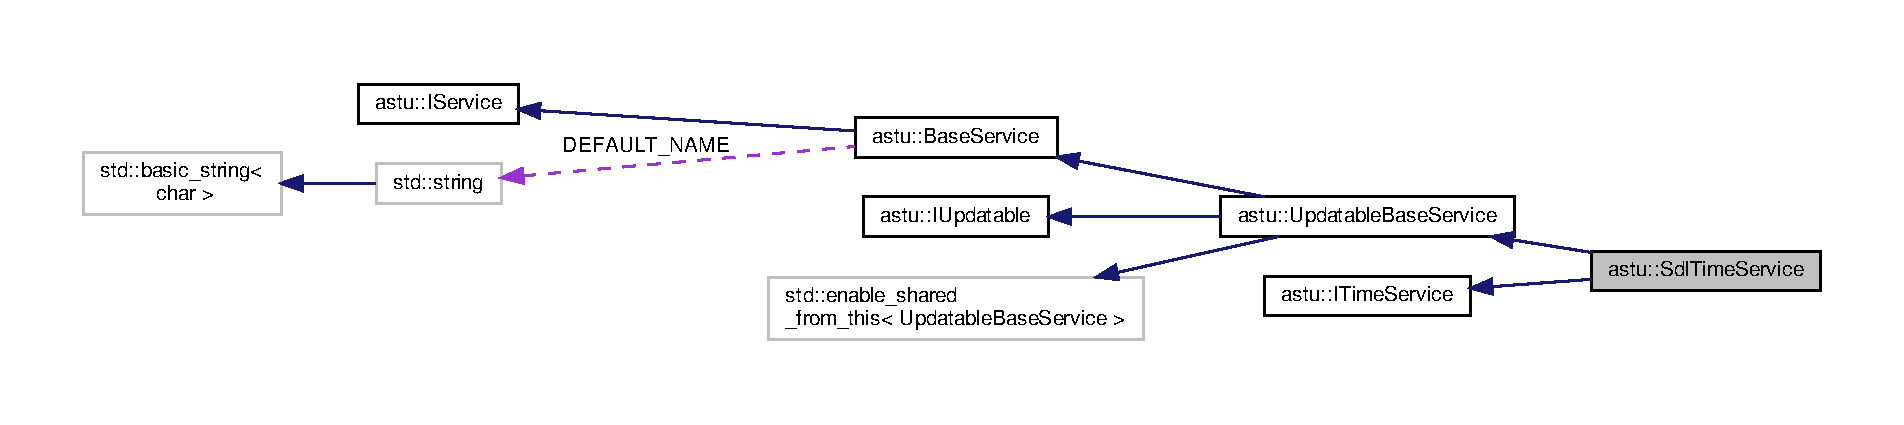
\includegraphics[width=350pt]{classastu_1_1SdlTimeService__coll__graph}
\end{center}
\end{figure}
\subsection*{Public Member Functions}
\begin{DoxyCompactItemize}
\item 
\hyperlink{classastu_1_1SdlTimeService_a66fa9afe98778d34ab4f2a92ba6ded40}{Sdl\+Time\+Service} (int priority=0)
\item 
\hyperlink{classastu_1_1SdlTimeService_a2e7171a77afc5bf3a051eba2b583ea8a}{$\sim$\+Sdl\+Time\+Service} ()
\item 
virtual double \hyperlink{classastu_1_1SdlTimeService_a6652d19cae14e20ec85a1808fc8e87b7}{Get\+Elapsed\+Time} () const override
\end{DoxyCompactItemize}
\subsection*{Protected Member Functions}
\begin{DoxyCompactItemize}
\item 
virtual void \hyperlink{classastu_1_1SdlTimeService_ac11551691bb14289020028a2a162c7d6}{On\+Startup} () override
\item 
virtual void \hyperlink{classastu_1_1SdlTimeService_a6a1b864beed186413933dd8b97a393a2}{On\+Shutdown} () override
\item 
virtual void \hyperlink{classastu_1_1SdlTimeService_ada8347f0f665616a2202919e71b76302}{On\+Update} () override
\end{DoxyCompactItemize}
\subsection*{Additional Inherited Members}


\subsection{Detailed Description}
Uses the S\+DL high performance timer to measure elapsed time. 

\subsection{Constructor \& Destructor Documentation}
\mbox{\Hypertarget{classastu_1_1SdlTimeService_a66fa9afe98778d34ab4f2a92ba6ded40}\label{classastu_1_1SdlTimeService_a66fa9afe98778d34ab4f2a92ba6ded40}} 
\index{astu\+::\+Sdl\+Time\+Service@{astu\+::\+Sdl\+Time\+Service}!Sdl\+Time\+Service@{Sdl\+Time\+Service}}
\index{Sdl\+Time\+Service@{Sdl\+Time\+Service}!astu\+::\+Sdl\+Time\+Service@{astu\+::\+Sdl\+Time\+Service}}
\subsubsection{\texorpdfstring{Sdl\+Time\+Service()}{SdlTimeService()}}
{\footnotesize\ttfamily astu\+::\+Sdl\+Time\+Service\+::\+Sdl\+Time\+Service (\begin{DoxyParamCaption}\item[{int}]{priority = {\ttfamily 0} }\end{DoxyParamCaption})}

Constructor.


\begin{DoxyParams}{Parameters}
{\em priority} & the priority used to update this service \\
\hline
\end{DoxyParams}
\mbox{\Hypertarget{classastu_1_1SdlTimeService_a2e7171a77afc5bf3a051eba2b583ea8a}\label{classastu_1_1SdlTimeService_a2e7171a77afc5bf3a051eba2b583ea8a}} 
\index{astu\+::\+Sdl\+Time\+Service@{astu\+::\+Sdl\+Time\+Service}!````~Sdl\+Time\+Service@{$\sim$\+Sdl\+Time\+Service}}
\index{````~Sdl\+Time\+Service@{$\sim$\+Sdl\+Time\+Service}!astu\+::\+Sdl\+Time\+Service@{astu\+::\+Sdl\+Time\+Service}}
\subsubsection{\texorpdfstring{$\sim$\+Sdl\+Time\+Service()}{~SdlTimeService()}}
{\footnotesize\ttfamily astu\+::\+Sdl\+Time\+Service\+::$\sim$\+Sdl\+Time\+Service (\begin{DoxyParamCaption}{ }\end{DoxyParamCaption})\hspace{0.3cm}{\ttfamily [inline]}}

Virtual destructor. 

\subsection{Member Function Documentation}
\mbox{\Hypertarget{classastu_1_1SdlTimeService_a6652d19cae14e20ec85a1808fc8e87b7}\label{classastu_1_1SdlTimeService_a6652d19cae14e20ec85a1808fc8e87b7}} 
\index{astu\+::\+Sdl\+Time\+Service@{astu\+::\+Sdl\+Time\+Service}!Get\+Elapsed\+Time@{Get\+Elapsed\+Time}}
\index{Get\+Elapsed\+Time@{Get\+Elapsed\+Time}!astu\+::\+Sdl\+Time\+Service@{astu\+::\+Sdl\+Time\+Service}}
\subsubsection{\texorpdfstring{Get\+Elapsed\+Time()}{GetElapsedTime()}}
{\footnotesize\ttfamily virtual double astu\+::\+Sdl\+Time\+Service\+::\+Get\+Elapsed\+Time (\begin{DoxyParamCaption}{ }\end{DoxyParamCaption}) const\hspace{0.3cm}{\ttfamily [override]}, {\ttfamily [virtual]}}

Returns the elapsed time since the last update.


\begin{DoxyParams}{Parameters}
{\em double} & the elapsed time in seconds \\
\hline
\end{DoxyParams}


Implements \hyperlink{classastu_1_1ITimeService_af38c6c5f4fedc705c14b01f2c61b0afc}{astu\+::\+I\+Time\+Service}.

\mbox{\Hypertarget{classastu_1_1SdlTimeService_a6a1b864beed186413933dd8b97a393a2}\label{classastu_1_1SdlTimeService_a6a1b864beed186413933dd8b97a393a2}} 
\index{astu\+::\+Sdl\+Time\+Service@{astu\+::\+Sdl\+Time\+Service}!On\+Shutdown@{On\+Shutdown}}
\index{On\+Shutdown@{On\+Shutdown}!astu\+::\+Sdl\+Time\+Service@{astu\+::\+Sdl\+Time\+Service}}
\subsubsection{\texorpdfstring{On\+Shutdown()}{OnShutdown()}}
{\footnotesize\ttfamily virtual void astu\+::\+Sdl\+Time\+Service\+::\+On\+Shutdown (\begin{DoxyParamCaption}{ }\end{DoxyParamCaption})\hspace{0.3cm}{\ttfamily [override]}, {\ttfamily [protected]}, {\ttfamily [virtual]}}

Called by this base class on shutdown.

Derived classes should override this method rather than {\ttfamily \hyperlink{classastu_1_1UpdatableBaseService_a7ad7e0201007878b6014361dd5ba82f9}{Shutdown()}}. The {\ttfamily \hyperlink{classastu_1_1UpdatableBaseService_a7ad7e0201007878b6014361dd5ba82f9}{Shutdown()}} method is maintaining the running-\/state of this service. 

Reimplemented from \hyperlink{classastu_1_1BaseService_aeb5003f7c5efe5412725ac4c66942d03}{astu\+::\+Base\+Service}.

\mbox{\Hypertarget{classastu_1_1SdlTimeService_ac11551691bb14289020028a2a162c7d6}\label{classastu_1_1SdlTimeService_ac11551691bb14289020028a2a162c7d6}} 
\index{astu\+::\+Sdl\+Time\+Service@{astu\+::\+Sdl\+Time\+Service}!On\+Startup@{On\+Startup}}
\index{On\+Startup@{On\+Startup}!astu\+::\+Sdl\+Time\+Service@{astu\+::\+Sdl\+Time\+Service}}
\subsubsection{\texorpdfstring{On\+Startup()}{OnStartup()}}
{\footnotesize\ttfamily virtual void astu\+::\+Sdl\+Time\+Service\+::\+On\+Startup (\begin{DoxyParamCaption}{ }\end{DoxyParamCaption})\hspace{0.3cm}{\ttfamily [override]}, {\ttfamily [protected]}, {\ttfamily [virtual]}}

Called by this base class on startup.

Derived classes should override this method rather than {\ttfamily \hyperlink{classastu_1_1UpdatableBaseService_a47e3725f717cee3cd8983f485b2a0243}{Startup()}}. The {\ttfamily \hyperlink{classastu_1_1UpdatableBaseService_a47e3725f717cee3cd8983f485b2a0243}{Startup()}} method is maintaining the running-\/state of this service. 

Reimplemented from \hyperlink{classastu_1_1BaseService_ac8710cd2d6dcc990db65e7c8ccfbc5ff}{astu\+::\+Base\+Service}.

\mbox{\Hypertarget{classastu_1_1SdlTimeService_ada8347f0f665616a2202919e71b76302}\label{classastu_1_1SdlTimeService_ada8347f0f665616a2202919e71b76302}} 
\index{astu\+::\+Sdl\+Time\+Service@{astu\+::\+Sdl\+Time\+Service}!On\+Update@{On\+Update}}
\index{On\+Update@{On\+Update}!astu\+::\+Sdl\+Time\+Service@{astu\+::\+Sdl\+Time\+Service}}
\subsubsection{\texorpdfstring{On\+Update()}{OnUpdate()}}
{\footnotesize\ttfamily virtual void astu\+::\+Sdl\+Time\+Service\+::\+On\+Update (\begin{DoxyParamCaption}{ }\end{DoxyParamCaption})\hspace{0.3cm}{\ttfamily [override]}, {\ttfamily [protected]}, {\ttfamily [virtual]}}

Called when this updatable gets updated. 

Implements \hyperlink{classastu_1_1IUpdatable_a76c7c6e2a71b725bbdbdf6808ef4743f}{astu\+::\+I\+Updatable}.



The documentation for this class was generated from the following file\+:\begin{DoxyCompactItemize}
\item 
include/Sdl\+Time\+Service.\+h\end{DoxyCompactItemize}

\hypertarget{classastu_1_1SdlVideoService}{}\section{astu\+:\+:Sdl\+Video\+Service Class Reference}
\label{classastu_1_1SdlVideoService}\index{astu\+::\+Sdl\+Video\+Service@{astu\+::\+Sdl\+Video\+Service}}


{\ttfamily \#include $<$Sdl\+Video\+Service.\+h$>$}



Inheritance diagram for astu\+:\+:Sdl\+Video\+Service\+:\nopagebreak
\begin{figure}[H]
\begin{center}
\leavevmode
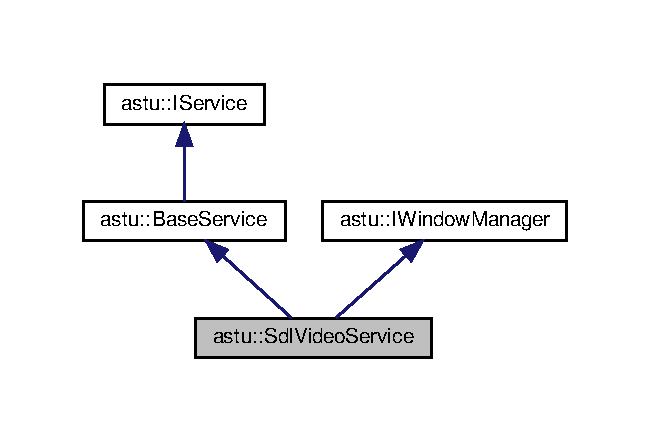
\includegraphics[width=350pt]{classastu_1_1SdlVideoService__inherit__graph}
\end{center}
\end{figure}


Collaboration diagram for astu\+:\+:Sdl\+Video\+Service\+:\nopagebreak
\begin{figure}[H]
\begin{center}
\leavevmode
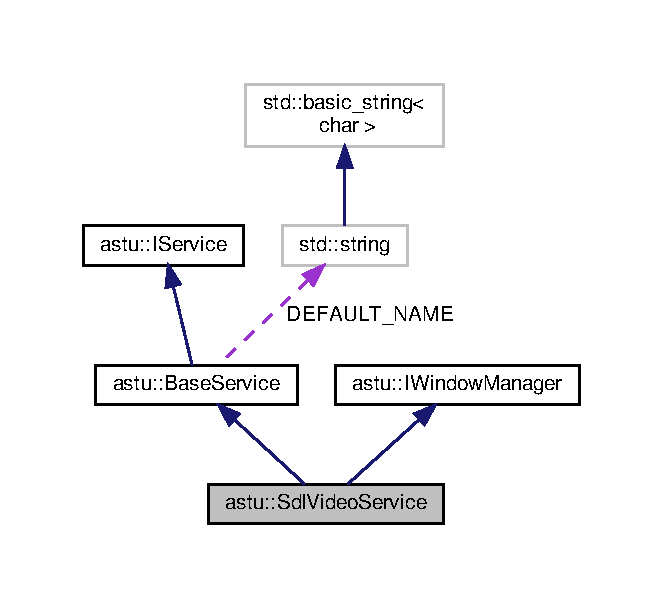
\includegraphics[width=350pt]{classastu_1_1SdlVideoService__coll__graph}
\end{center}
\end{figure}
\subsection*{Public Member Functions}
\begin{DoxyCompactItemize}
\item 
\hyperlink{classastu_1_1SdlVideoService_a21f04798e41b0c5c083acc1eefcbb5c1}{Sdl\+Video\+Service} ()
\item 
virtual \hyperlink{classastu_1_1SdlVideoService_a5ab48fd8569c517151099d71a86cc0b5}{$\sim$\+Sdl\+Video\+Service} ()
\item 
S\+D\+L\+\_\+\+Window $\ast$ \hyperlink{classastu_1_1SdlVideoService_af0282450cc95c0cbc2a6add84603dd7a}{Get\+Sdl\+Window} ()
\item 
bool \hyperlink{classastu_1_1SdlVideoService_aa40bb996597ad6c1005ce9dfd632cf28}{Is\+Vulkan\+Support\+Enabled} () const
\item 
\hyperlink{classastu_1_1SdlVideoService}{Sdl\+Video\+Service} \& \hyperlink{classastu_1_1SdlVideoService_a1ffb1c36698630d153b50b37cb1bcaee}{Enable\+Vulkan\+Support} (bool b)
\item 
\hyperlink{classastu_1_1SdlVideoService}{Sdl\+Video\+Service} \& \hyperlink{classastu_1_1SdlVideoService_a46fe8816a8975a2d6cd7311bdbd46167}{Set\+Display} (int idx)
\item 
virtual void \hyperlink{classastu_1_1SdlVideoService_a1c8d729ef42024bc0cc5065ecc6631c8}{Set\+Size} (int width, int height) override
\item 
virtual int \hyperlink{classastu_1_1SdlVideoService_a45c3181611e718bcfe44862baed6d520}{Get\+Width} () const override
\item 
virtual int \hyperlink{classastu_1_1SdlVideoService_a76d0f56254c9545d4d9762349133d4af}{Get\+Height} () const override
\item 
virtual void \hyperlink{classastu_1_1SdlVideoService_aad3c873db481dd622d6ddcea70b279af}{Set\+Title} (const std\+::string \&title) override
\item 
virtual const std\+::string \& \hyperlink{classastu_1_1SdlVideoService_ad6ee7f7a409960e91ddd77bbcea6432f}{Get\+Title} () const override
\item 
virtual void \hyperlink{classastu_1_1SdlVideoService_ab50969b38dedf29146704898a74df5ae}{Set\+Resizable} (bool b) override
\item 
virtual bool \hyperlink{classastu_1_1SdlVideoService_a335762da99b341205b8bf759a0b57c64}{Is\+Resizable} () const override
\item 
virtual int \hyperlink{classastu_1_1SdlVideoService_a3aefc8ab3780a23cdef8780e42436fd5}{Num\+Displays} () const override
\item 
virtual void \hyperlink{classastu_1_1SdlVideoService_a45a37b4958f6e77e22ffa55699a171ef}{Set\+Fullscreen} (bool b) override
\item 
virtual bool \hyperlink{classastu_1_1SdlVideoService_ae2be9aedf021799802cf7d1feaef7dfc}{Is\+Fullscreen} () const override
\end{DoxyCompactItemize}
\subsection*{Protected Member Functions}
\begin{DoxyCompactItemize}
\item 
virtual void \hyperlink{classastu_1_1SdlVideoService_add229ac2af59a4aea090e4de4c67e530}{On\+Startup} () override
\item 
virtual void \hyperlink{classastu_1_1SdlVideoService_a6d6085e9ff213c5d41546d604ff53e92}{On\+Shutdown} () override
\end{DoxyCompactItemize}
\subsection*{Additional Inherited Members}


\subsection{Detailed Description}
Initializes and opens the S\+D\+L-\/based main application window.

This service initializes the video submodule of S\+DL and maintains the main application window. 

\subsection{Constructor \& Destructor Documentation}
\mbox{\Hypertarget{classastu_1_1SdlVideoService_a21f04798e41b0c5c083acc1eefcbb5c1}\label{classastu_1_1SdlVideoService_a21f04798e41b0c5c083acc1eefcbb5c1}} 
\index{astu\+::\+Sdl\+Video\+Service@{astu\+::\+Sdl\+Video\+Service}!Sdl\+Video\+Service@{Sdl\+Video\+Service}}
\index{Sdl\+Video\+Service@{Sdl\+Video\+Service}!astu\+::\+Sdl\+Video\+Service@{astu\+::\+Sdl\+Video\+Service}}
\subsubsection{\texorpdfstring{Sdl\+Video\+Service()}{SdlVideoService()}}
{\footnotesize\ttfamily astu\+::\+Sdl\+Video\+Service\+::\+Sdl\+Video\+Service (\begin{DoxyParamCaption}{ }\end{DoxyParamCaption})}

Constructor. \mbox{\Hypertarget{classastu_1_1SdlVideoService_a5ab48fd8569c517151099d71a86cc0b5}\label{classastu_1_1SdlVideoService_a5ab48fd8569c517151099d71a86cc0b5}} 
\index{astu\+::\+Sdl\+Video\+Service@{astu\+::\+Sdl\+Video\+Service}!````~Sdl\+Video\+Service@{$\sim$\+Sdl\+Video\+Service}}
\index{````~Sdl\+Video\+Service@{$\sim$\+Sdl\+Video\+Service}!astu\+::\+Sdl\+Video\+Service@{astu\+::\+Sdl\+Video\+Service}}
\subsubsection{\texorpdfstring{$\sim$\+Sdl\+Video\+Service()}{~SdlVideoService()}}
{\footnotesize\ttfamily virtual astu\+::\+Sdl\+Video\+Service\+::$\sim$\+Sdl\+Video\+Service (\begin{DoxyParamCaption}{ }\end{DoxyParamCaption})\hspace{0.3cm}{\ttfamily [inline]}, {\ttfamily [virtual]}}

Virtual destructor. 

\subsection{Member Function Documentation}
\mbox{\Hypertarget{classastu_1_1SdlVideoService_a1ffb1c36698630d153b50b37cb1bcaee}\label{classastu_1_1SdlVideoService_a1ffb1c36698630d153b50b37cb1bcaee}} 
\index{astu\+::\+Sdl\+Video\+Service@{astu\+::\+Sdl\+Video\+Service}!Enable\+Vulkan\+Support@{Enable\+Vulkan\+Support}}
\index{Enable\+Vulkan\+Support@{Enable\+Vulkan\+Support}!astu\+::\+Sdl\+Video\+Service@{astu\+::\+Sdl\+Video\+Service}}
\subsubsection{\texorpdfstring{Enable\+Vulkan\+Support()}{EnableVulkanSupport()}}
{\footnotesize\ttfamily \hyperlink{classastu_1_1SdlVideoService}{Sdl\+Video\+Service}\& astu\+::\+Sdl\+Video\+Service\+::\+Enable\+Vulkan\+Support (\begin{DoxyParamCaption}\item[{bool}]{b }\end{DoxyParamCaption})}

Enables or disables Vulkan support.


\begin{DoxyParams}{Parameters}
{\em b} & set to {\ttfamily true} to enable Vulkan \\
\hline
\end{DoxyParams}
\begin{DoxyReturn}{Returns}
reference to this service for method chaining 
\end{DoxyReturn}

\begin{DoxyExceptions}{Exceptions}
{\em std\+::logic\+\_\+error} & in case this service is already running \\
\hline
\end{DoxyExceptions}
\mbox{\Hypertarget{classastu_1_1SdlVideoService_a76d0f56254c9545d4d9762349133d4af}\label{classastu_1_1SdlVideoService_a76d0f56254c9545d4d9762349133d4af}} 
\index{astu\+::\+Sdl\+Video\+Service@{astu\+::\+Sdl\+Video\+Service}!Get\+Height@{Get\+Height}}
\index{Get\+Height@{Get\+Height}!astu\+::\+Sdl\+Video\+Service@{astu\+::\+Sdl\+Video\+Service}}
\subsubsection{\texorpdfstring{Get\+Height()}{GetHeight()}}
{\footnotesize\ttfamily virtual int astu\+::\+Sdl\+Video\+Service\+::\+Get\+Height (\begin{DoxyParamCaption}{ }\end{DoxyParamCaption}) const\hspace{0.3cm}{\ttfamily [override]}, {\ttfamily [virtual]}}

Returns the height of the window in pixels.

\begin{DoxyReturn}{Returns}
the height in pixls 
\end{DoxyReturn}


Implements \hyperlink{classastu_1_1WindowService_a16d1880606a2c597162d8c80bed9d1a2}{astu\+::\+Window\+Service}.

\mbox{\Hypertarget{classastu_1_1SdlVideoService_af0282450cc95c0cbc2a6add84603dd7a}\label{classastu_1_1SdlVideoService_af0282450cc95c0cbc2a6add84603dd7a}} 
\index{astu\+::\+Sdl\+Video\+Service@{astu\+::\+Sdl\+Video\+Service}!Get\+Sdl\+Window@{Get\+Sdl\+Window}}
\index{Get\+Sdl\+Window@{Get\+Sdl\+Window}!astu\+::\+Sdl\+Video\+Service@{astu\+::\+Sdl\+Video\+Service}}
\subsubsection{\texorpdfstring{Get\+Sdl\+Window()}{GetSdlWindow()}}
{\footnotesize\ttfamily S\+D\+L\+\_\+\+Window$\ast$ astu\+::\+Sdl\+Video\+Service\+::\+Get\+Sdl\+Window (\begin{DoxyParamCaption}{ }\end{DoxyParamCaption})}

Returns a pointer to the S\+DL window structure.

This method is mostly used by other S\+DL services.

\begin{DoxyReturn}{Returns}
S\+D\+L\+\_\+\+Window the S\+DL window or {\ttfamily nullptr} if this service has not been started 
\end{DoxyReturn}
\mbox{\Hypertarget{classastu_1_1SdlVideoService_ad6ee7f7a409960e91ddd77bbcea6432f}\label{classastu_1_1SdlVideoService_ad6ee7f7a409960e91ddd77bbcea6432f}} 
\index{astu\+::\+Sdl\+Video\+Service@{astu\+::\+Sdl\+Video\+Service}!Get\+Title@{Get\+Title}}
\index{Get\+Title@{Get\+Title}!astu\+::\+Sdl\+Video\+Service@{astu\+::\+Sdl\+Video\+Service}}
\subsubsection{\texorpdfstring{Get\+Title()}{GetTitle()}}
{\footnotesize\ttfamily virtual const std\+::string\& astu\+::\+Sdl\+Video\+Service\+::\+Get\+Title (\begin{DoxyParamCaption}{ }\end{DoxyParamCaption}) const\hspace{0.3cm}{\ttfamily [override]}, {\ttfamily [virtual]}}

Returns the current window title.

\begin{DoxyReturn}{Returns}
the window title 
\end{DoxyReturn}


Implements \hyperlink{classastu_1_1WindowService_a54815692f9d3086673dd2694d75dcb65}{astu\+::\+Window\+Service}.

\mbox{\Hypertarget{classastu_1_1SdlVideoService_a45c3181611e718bcfe44862baed6d520}\label{classastu_1_1SdlVideoService_a45c3181611e718bcfe44862baed6d520}} 
\index{astu\+::\+Sdl\+Video\+Service@{astu\+::\+Sdl\+Video\+Service}!Get\+Width@{Get\+Width}}
\index{Get\+Width@{Get\+Width}!astu\+::\+Sdl\+Video\+Service@{astu\+::\+Sdl\+Video\+Service}}
\subsubsection{\texorpdfstring{Get\+Width()}{GetWidth()}}
{\footnotesize\ttfamily virtual int astu\+::\+Sdl\+Video\+Service\+::\+Get\+Width (\begin{DoxyParamCaption}{ }\end{DoxyParamCaption}) const\hspace{0.3cm}{\ttfamily [override]}, {\ttfamily [virtual]}}

Returns the width of the window in pixels.

\begin{DoxyReturn}{Returns}
the width in pixls 
\end{DoxyReturn}


Implements \hyperlink{classastu_1_1WindowService_ad2e75e91b0d72afb92c980fcbd8f227a}{astu\+::\+Window\+Service}.

\mbox{\Hypertarget{classastu_1_1SdlVideoService_ae2be9aedf021799802cf7d1feaef7dfc}\label{classastu_1_1SdlVideoService_ae2be9aedf021799802cf7d1feaef7dfc}} 
\index{astu\+::\+Sdl\+Video\+Service@{astu\+::\+Sdl\+Video\+Service}!Is\+Fullscreen@{Is\+Fullscreen}}
\index{Is\+Fullscreen@{Is\+Fullscreen}!astu\+::\+Sdl\+Video\+Service@{astu\+::\+Sdl\+Video\+Service}}
\subsubsection{\texorpdfstring{Is\+Fullscreen()}{IsFullscreen()}}
{\footnotesize\ttfamily virtual bool astu\+::\+Sdl\+Video\+Service\+::\+Is\+Fullscreen (\begin{DoxyParamCaption}{ }\end{DoxyParamCaption}) const\hspace{0.3cm}{\ttfamily [override]}, {\ttfamily [virtual]}}

Returns whether fullscreen mode is currently activated.

\begin{DoxyReturn}{Returns}
{\ttfamily true} if fulscreen mode is activated 
\end{DoxyReturn}


Implements \hyperlink{classastu_1_1WindowService_aa94ce60d1e8dd7484d364b65c25be1ca}{astu\+::\+Window\+Service}.

\mbox{\Hypertarget{classastu_1_1SdlVideoService_a335762da99b341205b8bf759a0b57c64}\label{classastu_1_1SdlVideoService_a335762da99b341205b8bf759a0b57c64}} 
\index{astu\+::\+Sdl\+Video\+Service@{astu\+::\+Sdl\+Video\+Service}!Is\+Resizable@{Is\+Resizable}}
\index{Is\+Resizable@{Is\+Resizable}!astu\+::\+Sdl\+Video\+Service@{astu\+::\+Sdl\+Video\+Service}}
\subsubsection{\texorpdfstring{Is\+Resizable()}{IsResizable()}}
{\footnotesize\ttfamily virtual bool astu\+::\+Sdl\+Video\+Service\+::\+Is\+Resizable (\begin{DoxyParamCaption}{ }\end{DoxyParamCaption}) const\hspace{0.3cm}{\ttfamily [override]}, {\ttfamily [virtual]}}

Returns whether the window is resizable.

\begin{DoxyReturn}{Returns}
{\ttfamily true} if the window is resizable 
\end{DoxyReturn}


Implements \hyperlink{classastu_1_1WindowService_a277954f71dd019b3ffc5d37df3f8b3af}{astu\+::\+Window\+Service}.

\mbox{\Hypertarget{classastu_1_1SdlVideoService_aa40bb996597ad6c1005ce9dfd632cf28}\label{classastu_1_1SdlVideoService_aa40bb996597ad6c1005ce9dfd632cf28}} 
\index{astu\+::\+Sdl\+Video\+Service@{astu\+::\+Sdl\+Video\+Service}!Is\+Vulkan\+Support\+Enabled@{Is\+Vulkan\+Support\+Enabled}}
\index{Is\+Vulkan\+Support\+Enabled@{Is\+Vulkan\+Support\+Enabled}!astu\+::\+Sdl\+Video\+Service@{astu\+::\+Sdl\+Video\+Service}}
\subsubsection{\texorpdfstring{Is\+Vulkan\+Support\+Enabled()}{IsVulkanSupportEnabled()}}
{\footnotesize\ttfamily bool astu\+::\+Sdl\+Video\+Service\+::\+Is\+Vulkan\+Support\+Enabled (\begin{DoxyParamCaption}{ }\end{DoxyParamCaption}) const}

Returns whether Vulkan support has been enabled.

\begin{DoxyReturn}{Returns}
{\ttfamily true} if support for Vulkan has been enabled 
\end{DoxyReturn}
\mbox{\Hypertarget{classastu_1_1SdlVideoService_a3aefc8ab3780a23cdef8780e42436fd5}\label{classastu_1_1SdlVideoService_a3aefc8ab3780a23cdef8780e42436fd5}} 
\index{astu\+::\+Sdl\+Video\+Service@{astu\+::\+Sdl\+Video\+Service}!Num\+Displays@{Num\+Displays}}
\index{Num\+Displays@{Num\+Displays}!astu\+::\+Sdl\+Video\+Service@{astu\+::\+Sdl\+Video\+Service}}
\subsubsection{\texorpdfstring{Num\+Displays()}{NumDisplays()}}
{\footnotesize\ttfamily virtual int astu\+::\+Sdl\+Video\+Service\+::\+Num\+Displays (\begin{DoxyParamCaption}{ }\end{DoxyParamCaption}) const\hspace{0.3cm}{\ttfamily [override]}, {\ttfamily [virtual]}}

Returns the number of available displays. 

Implements \hyperlink{classastu_1_1WindowService_ad773e0c567946e06ace76c016bb16349}{astu\+::\+Window\+Service}.

\mbox{\Hypertarget{classastu_1_1SdlVideoService_a6d6085e9ff213c5d41546d604ff53e92}\label{classastu_1_1SdlVideoService_a6d6085e9ff213c5d41546d604ff53e92}} 
\index{astu\+::\+Sdl\+Video\+Service@{astu\+::\+Sdl\+Video\+Service}!On\+Shutdown@{On\+Shutdown}}
\index{On\+Shutdown@{On\+Shutdown}!astu\+::\+Sdl\+Video\+Service@{astu\+::\+Sdl\+Video\+Service}}
\subsubsection{\texorpdfstring{On\+Shutdown()}{OnShutdown()}}
{\footnotesize\ttfamily virtual void astu\+::\+Sdl\+Video\+Service\+::\+On\+Shutdown (\begin{DoxyParamCaption}{ }\end{DoxyParamCaption})\hspace{0.3cm}{\ttfamily [override]}, {\ttfamily [protected]}, {\ttfamily [virtual]}}

Called by the service base method on shutdown.

Derived can override this method for de-\/initialization purposes, e.\+g., releasing resources, etc. 

Reimplemented from \hyperlink{classastu_1_1Service_a1e1dff727df791c57fae782d8a613c5f}{astu\+::\+Service}.

\mbox{\Hypertarget{classastu_1_1SdlVideoService_add229ac2af59a4aea090e4de4c67e530}\label{classastu_1_1SdlVideoService_add229ac2af59a4aea090e4de4c67e530}} 
\index{astu\+::\+Sdl\+Video\+Service@{astu\+::\+Sdl\+Video\+Service}!On\+Startup@{On\+Startup}}
\index{On\+Startup@{On\+Startup}!astu\+::\+Sdl\+Video\+Service@{astu\+::\+Sdl\+Video\+Service}}
\subsubsection{\texorpdfstring{On\+Startup()}{OnStartup()}}
{\footnotesize\ttfamily virtual void astu\+::\+Sdl\+Video\+Service\+::\+On\+Startup (\begin{DoxyParamCaption}{ }\end{DoxyParamCaption})\hspace{0.3cm}{\ttfamily [override]}, {\ttfamily [protected]}, {\ttfamily [virtual]}}

Called by the service base class on startup.

Derived can override this method for initialization purposes. 

Reimplemented from \hyperlink{classastu_1_1Service_a357dc663e000b1f086f681ec3c459bfe}{astu\+::\+Service}.

\mbox{\Hypertarget{classastu_1_1SdlVideoService_a46fe8816a8975a2d6cd7311bdbd46167}\label{classastu_1_1SdlVideoService_a46fe8816a8975a2d6cd7311bdbd46167}} 
\index{astu\+::\+Sdl\+Video\+Service@{astu\+::\+Sdl\+Video\+Service}!Set\+Display@{Set\+Display}}
\index{Set\+Display@{Set\+Display}!astu\+::\+Sdl\+Video\+Service@{astu\+::\+Sdl\+Video\+Service}}
\subsubsection{\texorpdfstring{Set\+Display()}{SetDisplay()}}
{\footnotesize\ttfamily \hyperlink{classastu_1_1SdlVideoService}{Sdl\+Video\+Service}\& astu\+::\+Sdl\+Video\+Service\+::\+Set\+Display (\begin{DoxyParamCaption}\item[{int}]{idx }\end{DoxyParamCaption})}

Sets the index of the display used to open the window.


\begin{DoxyParams}{Parameters}
{\em idx} & the index of the display. \\
\hline
\end{DoxyParams}
\begin{DoxyReturn}{Returns}
reference to this service for method chaining 
\end{DoxyReturn}
\mbox{\Hypertarget{classastu_1_1SdlVideoService_a45a37b4958f6e77e22ffa55699a171ef}\label{classastu_1_1SdlVideoService_a45a37b4958f6e77e22ffa55699a171ef}} 
\index{astu\+::\+Sdl\+Video\+Service@{astu\+::\+Sdl\+Video\+Service}!Set\+Fullscreen@{Set\+Fullscreen}}
\index{Set\+Fullscreen@{Set\+Fullscreen}!astu\+::\+Sdl\+Video\+Service@{astu\+::\+Sdl\+Video\+Service}}
\subsubsection{\texorpdfstring{Set\+Fullscreen()}{SetFullscreen()}}
{\footnotesize\ttfamily virtual void astu\+::\+Sdl\+Video\+Service\+::\+Set\+Fullscreen (\begin{DoxyParamCaption}\item[{bool}]{enable\+Fullscreen }\end{DoxyParamCaption})\hspace{0.3cm}{\ttfamily [override]}, {\ttfamily [virtual]}}

Activates or deactivates fullscreen mode.


\begin{DoxyParams}{Parameters}
{\em enable\+Fullscreen} & set to {\ttfamily true} to activate fullscreen mode \\
\hline
\end{DoxyParams}


Implements \hyperlink{classastu_1_1WindowService_abe2ef0eb9f42078676318945e15d2dce}{astu\+::\+Window\+Service}.

\mbox{\Hypertarget{classastu_1_1SdlVideoService_ab50969b38dedf29146704898a74df5ae}\label{classastu_1_1SdlVideoService_ab50969b38dedf29146704898a74df5ae}} 
\index{astu\+::\+Sdl\+Video\+Service@{astu\+::\+Sdl\+Video\+Service}!Set\+Resizable@{Set\+Resizable}}
\index{Set\+Resizable@{Set\+Resizable}!astu\+::\+Sdl\+Video\+Service@{astu\+::\+Sdl\+Video\+Service}}
\subsubsection{\texorpdfstring{Set\+Resizable()}{SetResizable()}}
{\footnotesize\ttfamily virtual void astu\+::\+Sdl\+Video\+Service\+::\+Set\+Resizable (\begin{DoxyParamCaption}\item[{bool}]{b }\end{DoxyParamCaption})\hspace{0.3cm}{\ttfamily [override]}, {\ttfamily [virtual]}}

Specifies whether the window should be resizable.


\begin{DoxyParams}{Parameters}
{\em b} & the {\ttfamily true} if the window should be resizable \\
\hline
\end{DoxyParams}


Implements \hyperlink{classastu_1_1WindowService_a78bee95831f4497fcee7b8d10575f0d8}{astu\+::\+Window\+Service}.

\mbox{\Hypertarget{classastu_1_1SdlVideoService_a1c8d729ef42024bc0cc5065ecc6631c8}\label{classastu_1_1SdlVideoService_a1c8d729ef42024bc0cc5065ecc6631c8}} 
\index{astu\+::\+Sdl\+Video\+Service@{astu\+::\+Sdl\+Video\+Service}!Set\+Size@{Set\+Size}}
\index{Set\+Size@{Set\+Size}!astu\+::\+Sdl\+Video\+Service@{astu\+::\+Sdl\+Video\+Service}}
\subsubsection{\texorpdfstring{Set\+Size()}{SetSize()}}
{\footnotesize\ttfamily virtual void astu\+::\+Sdl\+Video\+Service\+::\+Set\+Size (\begin{DoxyParamCaption}\item[{int}]{width,  }\item[{int}]{height }\end{DoxyParamCaption})\hspace{0.3cm}{\ttfamily [override]}, {\ttfamily [virtual]}}

Sets the dimension of the window.


\begin{DoxyParams}{Parameters}
{\em width} & the width of the window in pixels \\
\hline
{\em height} & the height of the window in pixels \\
\hline
\end{DoxyParams}


Implements \hyperlink{classastu_1_1WindowService_a77fb8b7272b58e39c7d003923034eedf}{astu\+::\+Window\+Service}.

\mbox{\Hypertarget{classastu_1_1SdlVideoService_aad3c873db481dd622d6ddcea70b279af}\label{classastu_1_1SdlVideoService_aad3c873db481dd622d6ddcea70b279af}} 
\index{astu\+::\+Sdl\+Video\+Service@{astu\+::\+Sdl\+Video\+Service}!Set\+Title@{Set\+Title}}
\index{Set\+Title@{Set\+Title}!astu\+::\+Sdl\+Video\+Service@{astu\+::\+Sdl\+Video\+Service}}
\subsubsection{\texorpdfstring{Set\+Title()}{SetTitle()}}
{\footnotesize\ttfamily virtual void astu\+::\+Sdl\+Video\+Service\+::\+Set\+Title (\begin{DoxyParamCaption}\item[{const std\+::string \&}]{title }\end{DoxyParamCaption})\hspace{0.3cm}{\ttfamily [override]}, {\ttfamily [virtual]}}

Sets the window title.


\begin{DoxyParams}{Parameters}
{\em title} & the title of the window \\
\hline
\end{DoxyParams}


Implements \hyperlink{classastu_1_1WindowService_a298dcaad372f611f14edb4ad33044efd}{astu\+::\+Window\+Service}.



The documentation for this class was generated from the following file\+:\begin{DoxyCompactItemize}
\item 
include/\+Suite\+S\+D\+L/Sdl\+Video\+Service.\+h\end{DoxyCompactItemize}

\hypertarget{classastu_1_1ServiceManager}{}\section{astu\+:\+:Service\+Manager Class Reference}
\label{classastu_1_1ServiceManager}\index{astu\+::\+Service\+Manager@{astu\+::\+Service\+Manager}}


{\ttfamily \#include $<$Service\+Manager.\+h$>$}

\subsection*{Public Member Functions}
\begin{DoxyCompactItemize}
\item 
void \hyperlink{classastu_1_1ServiceManager_a274475bef03cea4810f98082cdb24295}{Add\+Service} (std\+::shared\+\_\+ptr$<$ \hyperlink{classastu_1_1Service}{Service} $>$ service)
\item 
void \hyperlink{classastu_1_1ServiceManager_adbab5f4a6e042604e2c51eefcf69f7b5}{Remove\+Service} (std\+::shared\+\_\+ptr$<$ \hyperlink{classastu_1_1Service}{Service} $>$ service)
\item 
void \hyperlink{classastu_1_1ServiceManager_ad94c3984be162a0d4e3633abd8b81099}{Remove\+All\+Services} ()
\item 
bool \hyperlink{classastu_1_1ServiceManager_ab8af7a024cea64d9f4f4431360641b16}{Has\+Service} (std\+::shared\+\_\+ptr$<$ \hyperlink{classastu_1_1Service}{Service} $>$ service) const
\item 
void \hyperlink{classastu_1_1ServiceManager_a7d4918c435a26a4212902ade5f9829b6}{Startup\+All} ()
\item 
void \hyperlink{classastu_1_1ServiceManager_a0ec3c06392ae4e7dab8d4b550bed1699}{Shutdown\+All} ()
\item 
bool \hyperlink{classastu_1_1ServiceManager_a64cea7132b9be6521a9af6f76009e5d4}{Is\+Running} () const
\item 
{\footnotesize template$<$typename T $>$ }\\std\+::shared\+\_\+ptr$<$ T $>$ \hyperlink{classastu_1_1ServiceManager_acef5ab6b48a9811b810851c69751f71a}{Find\+Service} ()
\item 
{\footnotesize template$<$typename T $>$ }\\std\+::shared\+\_\+ptr$<$ T $>$ \hyperlink{classastu_1_1ServiceManager_a3000933260f102748f75c9b4064fd119}{Find\+Service} (std\+::shared\+\_\+ptr$<$ T $>$ default\+Result)
\end{DoxyCompactItemize}
\subsection*{Static Public Member Functions}
\begin{DoxyCompactItemize}
\item 
static \hyperlink{classastu_1_1ServiceManager}{Service\+Manager} \& \hyperlink{classastu_1_1ServiceManager_a26941fe98ea3f2792deca62e4124bf15}{Get\+Instance} ()
\end{DoxyCompactItemize}


\subsection{Detailed Description}
\hyperlink{classastu_1_1Service}{Service} manager is used administer essential application-\/wide services.

This implementation realizes the service manager as a singleton. 

\subsection{Member Function Documentation}
\mbox{\Hypertarget{classastu_1_1ServiceManager_a274475bef03cea4810f98082cdb24295}\label{classastu_1_1ServiceManager_a274475bef03cea4810f98082cdb24295}} 
\index{astu\+::\+Service\+Manager@{astu\+::\+Service\+Manager}!Add\+Service@{Add\+Service}}
\index{Add\+Service@{Add\+Service}!astu\+::\+Service\+Manager@{astu\+::\+Service\+Manager}}
\subsubsection{\texorpdfstring{Add\+Service()}{AddService()}}
{\footnotesize\ttfamily void astu\+::\+Service\+Manager\+::\+Add\+Service (\begin{DoxyParamCaption}\item[{std\+::shared\+\_\+ptr$<$ \hyperlink{classastu_1_1Service}{Service} $>$}]{service }\end{DoxyParamCaption})}

Adds a service to this manager.


\begin{DoxyParams}{Parameters}
{\em service} & the service to add \\
\hline
\end{DoxyParams}

\begin{DoxyExceptions}{Exceptions}
{\em std\+::logic\+\_\+error} & in case the service has already been added \\
\hline
\end{DoxyExceptions}
\mbox{\Hypertarget{classastu_1_1ServiceManager_acef5ab6b48a9811b810851c69751f71a}\label{classastu_1_1ServiceManager_acef5ab6b48a9811b810851c69751f71a}} 
\index{astu\+::\+Service\+Manager@{astu\+::\+Service\+Manager}!Find\+Service@{Find\+Service}}
\index{Find\+Service@{Find\+Service}!astu\+::\+Service\+Manager@{astu\+::\+Service\+Manager}}
\subsubsection{\texorpdfstring{Find\+Service()}{FindService()}\hspace{0.1cm}{\footnotesize\ttfamily [1/2]}}
{\footnotesize\ttfamily template$<$typename T $>$ \\
std\+::shared\+\_\+ptr$<$T$>$ astu\+::\+Service\+Manager\+::\+Find\+Service (\begin{DoxyParamCaption}{ }\end{DoxyParamCaption})\hspace{0.3cm}{\ttfamily [inline]}}

Searches for a service of a certain type.

{\bfseries Example}


\begin{DoxyCode}
\textcolor{comment}{// Fetch reference to the one and only service manager.}
\textcolor{keyword}{auto} & sm = \hyperlink{classastu_1_1ServiceManager_a26941fe98ea3f2792deca62e4124bf15}{ServiceManager::GetInstance}();

\textcolor{comment}{// Get a (smart-) pointer to a service which implements a certain}
\textcolor{comment}{// interface, in this case the TimeService interface.}
\textcolor{keyword}{auto} timeSrv = sm.FindService<TimeService>();

\textcolor{comment}{// Use the time service.}
\textcolor{keywordtype}{double} dt = timeSrv->GetElapsedTime();
\end{DoxyCode}



\begin{DoxyTemplParams}{Template Parameters}
{\em T} & the type of service to look for \\
\hline
\end{DoxyTemplParams}
\begin{DoxyReturn}{Returns}
the requested service 
\end{DoxyReturn}

\begin{DoxyExceptions}{Exceptions}
{\em std\+::logic\+\_\+error} & in case the service could not be found \\
\hline
\end{DoxyExceptions}
\mbox{\Hypertarget{classastu_1_1ServiceManager_a3000933260f102748f75c9b4064fd119}\label{classastu_1_1ServiceManager_a3000933260f102748f75c9b4064fd119}} 
\index{astu\+::\+Service\+Manager@{astu\+::\+Service\+Manager}!Find\+Service@{Find\+Service}}
\index{Find\+Service@{Find\+Service}!astu\+::\+Service\+Manager@{astu\+::\+Service\+Manager}}
\subsubsection{\texorpdfstring{Find\+Service()}{FindService()}\hspace{0.1cm}{\footnotesize\ttfamily [2/2]}}
{\footnotesize\ttfamily template$<$typename T $>$ \\
std\+::shared\+\_\+ptr$<$T$>$ astu\+::\+Service\+Manager\+::\+Find\+Service (\begin{DoxyParamCaption}\item[{std\+::shared\+\_\+ptr$<$ T $>$}]{default\+Result }\end{DoxyParamCaption})\hspace{0.3cm}{\ttfamily [inline]}}

Searches for a service of a certain type.


\begin{DoxyTemplParams}{Template Parameters}
{\em T} & the type of service to look for \\
\hline
\end{DoxyTemplParams}

\begin{DoxyParams}{Parameters}
{\em default\+Result} & the default value if no appropriate service could be found \\
\hline
\end{DoxyParams}
\begin{DoxyReturn}{Returns}
the requested service or the specified default value 
\end{DoxyReturn}
\mbox{\Hypertarget{classastu_1_1ServiceManager_a26941fe98ea3f2792deca62e4124bf15}\label{classastu_1_1ServiceManager_a26941fe98ea3f2792deca62e4124bf15}} 
\index{astu\+::\+Service\+Manager@{astu\+::\+Service\+Manager}!Get\+Instance@{Get\+Instance}}
\index{Get\+Instance@{Get\+Instance}!astu\+::\+Service\+Manager@{astu\+::\+Service\+Manager}}
\subsubsection{\texorpdfstring{Get\+Instance()}{GetInstance()}}
{\footnotesize\ttfamily static \hyperlink{classastu_1_1ServiceManager}{Service\+Manager}\& astu\+::\+Service\+Manager\+::\+Get\+Instance (\begin{DoxyParamCaption}{ }\end{DoxyParamCaption})\hspace{0.3cm}{\ttfamily [static]}}

Returns the one and only instance of the service manager.

\begin{DoxyReturn}{Returns}
the one and only service manager 
\end{DoxyReturn}
\mbox{\Hypertarget{classastu_1_1ServiceManager_ab8af7a024cea64d9f4f4431360641b16}\label{classastu_1_1ServiceManager_ab8af7a024cea64d9f4f4431360641b16}} 
\index{astu\+::\+Service\+Manager@{astu\+::\+Service\+Manager}!Has\+Service@{Has\+Service}}
\index{Has\+Service@{Has\+Service}!astu\+::\+Service\+Manager@{astu\+::\+Service\+Manager}}
\subsubsection{\texorpdfstring{Has\+Service()}{HasService()}}
{\footnotesize\ttfamily bool astu\+::\+Service\+Manager\+::\+Has\+Service (\begin{DoxyParamCaption}\item[{std\+::shared\+\_\+ptr$<$ \hyperlink{classastu_1_1Service}{Service} $>$}]{service }\end{DoxyParamCaption}) const}

Tests whether the specified services has already been added.


\begin{DoxyParams}{Parameters}
{\em service} & the service to test \\
\hline
\end{DoxyParams}
\begin{DoxyReturn}{Returns}
{\ttfamily true} in case the service has already been added 
\end{DoxyReturn}
\mbox{\Hypertarget{classastu_1_1ServiceManager_a64cea7132b9be6521a9af6f76009e5d4}\label{classastu_1_1ServiceManager_a64cea7132b9be6521a9af6f76009e5d4}} 
\index{astu\+::\+Service\+Manager@{astu\+::\+Service\+Manager}!Is\+Running@{Is\+Running}}
\index{Is\+Running@{Is\+Running}!astu\+::\+Service\+Manager@{astu\+::\+Service\+Manager}}
\subsubsection{\texorpdfstring{Is\+Running()}{IsRunning()}}
{\footnotesize\ttfamily bool astu\+::\+Service\+Manager\+::\+Is\+Running (\begin{DoxyParamCaption}{ }\end{DoxyParamCaption}) const}

Returns whether the services have been started.

\begin{DoxyReturn}{Returns}
{\ttfamily true} if the services have been started 
\end{DoxyReturn}
\mbox{\Hypertarget{classastu_1_1ServiceManager_ad94c3984be162a0d4e3633abd8b81099}\label{classastu_1_1ServiceManager_ad94c3984be162a0d4e3633abd8b81099}} 
\index{astu\+::\+Service\+Manager@{astu\+::\+Service\+Manager}!Remove\+All\+Services@{Remove\+All\+Services}}
\index{Remove\+All\+Services@{Remove\+All\+Services}!astu\+::\+Service\+Manager@{astu\+::\+Service\+Manager}}
\subsubsection{\texorpdfstring{Remove\+All\+Services()}{RemoveAllServices()}}
{\footnotesize\ttfamily void astu\+::\+Service\+Manager\+::\+Remove\+All\+Services (\begin{DoxyParamCaption}{ }\end{DoxyParamCaption})}

Removes all services. \mbox{\Hypertarget{classastu_1_1ServiceManager_adbab5f4a6e042604e2c51eefcf69f7b5}\label{classastu_1_1ServiceManager_adbab5f4a6e042604e2c51eefcf69f7b5}} 
\index{astu\+::\+Service\+Manager@{astu\+::\+Service\+Manager}!Remove\+Service@{Remove\+Service}}
\index{Remove\+Service@{Remove\+Service}!astu\+::\+Service\+Manager@{astu\+::\+Service\+Manager}}
\subsubsection{\texorpdfstring{Remove\+Service()}{RemoveService()}}
{\footnotesize\ttfamily void astu\+::\+Service\+Manager\+::\+Remove\+Service (\begin{DoxyParamCaption}\item[{std\+::shared\+\_\+ptr$<$ \hyperlink{classastu_1_1Service}{Service} $>$}]{service }\end{DoxyParamCaption})}

Removes the specified service.


\begin{DoxyParams}{Parameters}
{\em service} & the service to remove \\
\hline
\end{DoxyParams}
\mbox{\Hypertarget{classastu_1_1ServiceManager_a0ec3c06392ae4e7dab8d4b550bed1699}\label{classastu_1_1ServiceManager_a0ec3c06392ae4e7dab8d4b550bed1699}} 
\index{astu\+::\+Service\+Manager@{astu\+::\+Service\+Manager}!Shutdown\+All@{Shutdown\+All}}
\index{Shutdown\+All@{Shutdown\+All}!astu\+::\+Service\+Manager@{astu\+::\+Service\+Manager}}
\subsubsection{\texorpdfstring{Shutdown\+All()}{ShutdownAll()}}
{\footnotesize\ttfamily void astu\+::\+Service\+Manager\+::\+Shutdown\+All (\begin{DoxyParamCaption}{ }\end{DoxyParamCaption})}

Shuts down all services. \mbox{\Hypertarget{classastu_1_1ServiceManager_a7d4918c435a26a4212902ade5f9829b6}\label{classastu_1_1ServiceManager_a7d4918c435a26a4212902ade5f9829b6}} 
\index{astu\+::\+Service\+Manager@{astu\+::\+Service\+Manager}!Startup\+All@{Startup\+All}}
\index{Startup\+All@{Startup\+All}!astu\+::\+Service\+Manager@{astu\+::\+Service\+Manager}}
\subsubsection{\texorpdfstring{Startup\+All()}{StartupAll()}}
{\footnotesize\ttfamily void astu\+::\+Service\+Manager\+::\+Startup\+All (\begin{DoxyParamCaption}{ }\end{DoxyParamCaption})}

Starts up all services. 

The documentation for this class was generated from the following file\+:\begin{DoxyCompactItemize}
\item 
include/\+Service/Service\+Manager.\+h\end{DoxyCompactItemize}

\hypertarget{classastu_1_1SignalService}{}\section{astu\+:\+:Signal\+Service$<$ T $>$ Class Template Reference}
\label{classastu_1_1SignalService}\index{astu\+::\+Signal\+Service$<$ T $>$@{astu\+::\+Signal\+Service$<$ T $>$}}


{\ttfamily \#include $<$Signal\+Service.\+h$>$}



Inheritance diagram for astu\+:\+:Signal\+Service$<$ T $>$\+:\nopagebreak
\begin{figure}[H]
\begin{center}
\leavevmode
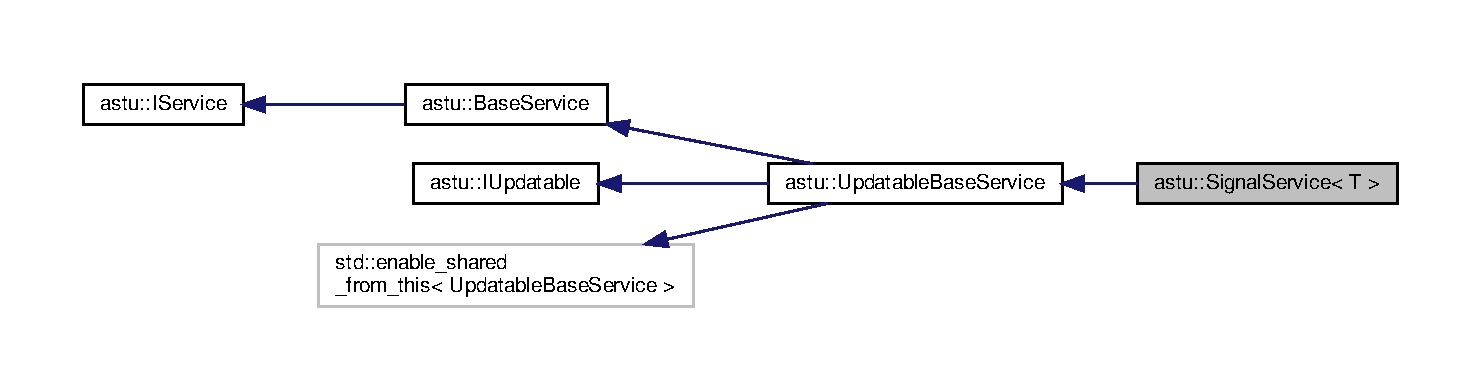
\includegraphics[width=350pt]{classastu_1_1SignalService__inherit__graph}
\end{center}
\end{figure}


Collaboration diagram for astu\+:\+:Signal\+Service$<$ T $>$\+:\nopagebreak
\begin{figure}[H]
\begin{center}
\leavevmode
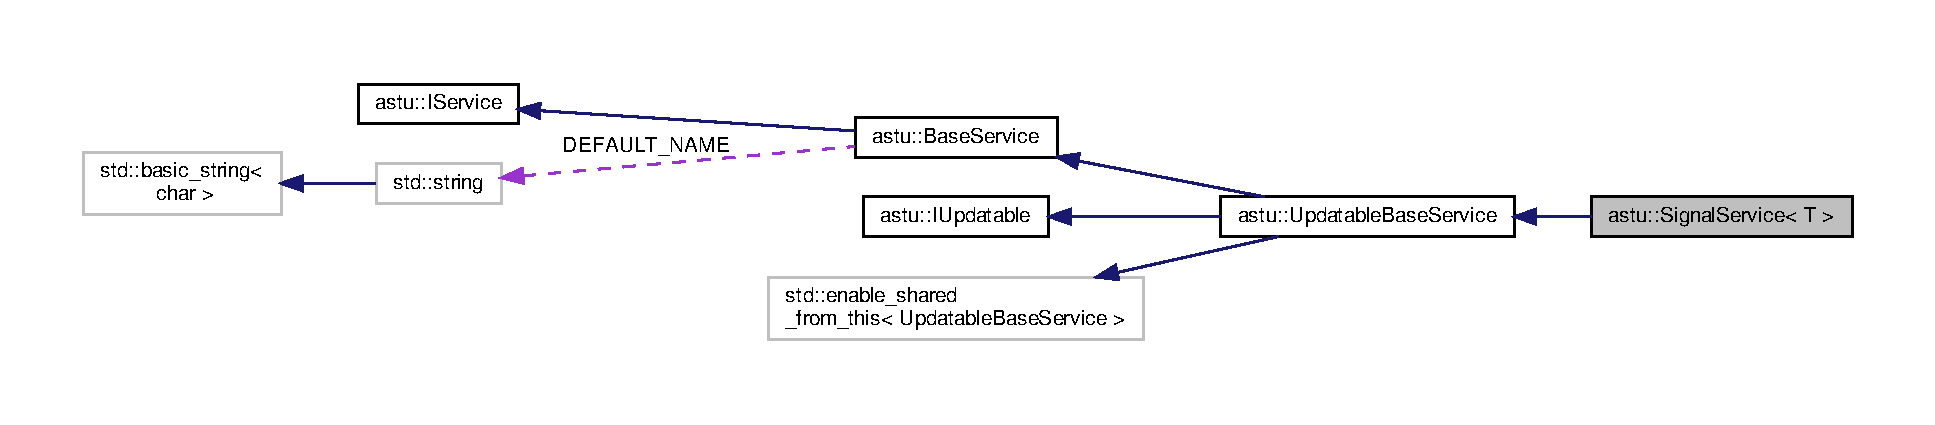
\includegraphics[width=350pt]{classastu_1_1SignalService__coll__graph}
\end{center}
\end{figure}
\subsection*{Public Member Functions}
\begin{DoxyCompactItemize}
\item 
\hyperlink{classastu_1_1SignalService_acf4e3bfbacc9eb6654a84d59b3ff1a6a}{Signal\+Service} (const std\+::string \&name=\hyperlink{classastu_1_1BaseService_a9483b26ad631bd14646ef2d2170cd828}{D\+E\+F\+A\+U\+L\+T\+\_\+\+N\+A\+ME}, int priority=0)
\item 
void \hyperlink{classastu_1_1SignalService_aa028a039b066a779af3834ffb3bdaa18}{Queue\+Signal} (const T \&signal)
\item 
void \hyperlink{classastu_1_1SignalService_a3ead09955e8e76bbdd6d9e5a853e88af}{Fire\+Signal} (const T \&signal)
\item 
void \hyperlink{classastu_1_1SignalService_a9027644028616eb9bad00447648cae29}{Add\+Listener} (const std\+::shared\+\_\+ptr$<$ \hyperlink{classastu_1_1ISignalListener}{I\+Signal\+Listener}$<$ T $>$$>$ \&listener)
\item 
void \hyperlink{classastu_1_1SignalService_aea0777f0393a7f3c4dafff9d58934194}{Remove\+Listener} (const std\+::shared\+\_\+ptr$<$ \hyperlink{classastu_1_1ISignalListener}{I\+Signal\+Listener}$<$ T $>$$>$ \&listener)
\item 
bool \hyperlink{classastu_1_1SignalService_acc4935715afef10b89fd905e714be389}{Has\+Listener} (const std\+::shared\+\_\+ptr$<$ \hyperlink{classastu_1_1ISignalListener}{I\+Signal\+Listener}$<$ T $>$$>$ \&listener) const
\end{DoxyCompactItemize}
\subsection*{Additional Inherited Members}


\subsection{Detailed Description}
\subsubsection*{template$<$typename T$>$\newline
class astu\+::\+Signal\+Service$<$ T $>$}

A template-\/based service which is used to transmit objects called \char`\"{}signals\char`\"{} to registered listeners. 

\subsection{Constructor \& Destructor Documentation}
\mbox{\Hypertarget{classastu_1_1SignalService_acf4e3bfbacc9eb6654a84d59b3ff1a6a}\label{classastu_1_1SignalService_acf4e3bfbacc9eb6654a84d59b3ff1a6a}} 
\index{astu\+::\+Signal\+Service@{astu\+::\+Signal\+Service}!Signal\+Service@{Signal\+Service}}
\index{Signal\+Service@{Signal\+Service}!astu\+::\+Signal\+Service@{astu\+::\+Signal\+Service}}
\subsubsection{\texorpdfstring{Signal\+Service()}{SignalService()}}
{\footnotesize\ttfamily template$<$typename T $>$ \\
\hyperlink{classastu_1_1SignalService}{astu\+::\+Signal\+Service}$<$ T $>$\+::\hyperlink{classastu_1_1SignalService}{Signal\+Service} (\begin{DoxyParamCaption}\item[{const std\+::string \&}]{name = {\ttfamily \hyperlink{classastu_1_1BaseService_a9483b26ad631bd14646ef2d2170cd828}{D\+E\+F\+A\+U\+L\+T\+\_\+\+N\+A\+ME}},  }\item[{int}]{priority = {\ttfamily 0} }\end{DoxyParamCaption})\hspace{0.3cm}{\ttfamily [inline]}}

Constructor.


\begin{DoxyParams}{Parameters}
{\em name} & the name of this service \\
\hline
{\em priority} & the update priority of this service \\
\hline
\end{DoxyParams}


\subsection{Member Function Documentation}
\mbox{\Hypertarget{classastu_1_1SignalService_a9027644028616eb9bad00447648cae29}\label{classastu_1_1SignalService_a9027644028616eb9bad00447648cae29}} 
\index{astu\+::\+Signal\+Service@{astu\+::\+Signal\+Service}!Add\+Listener@{Add\+Listener}}
\index{Add\+Listener@{Add\+Listener}!astu\+::\+Signal\+Service@{astu\+::\+Signal\+Service}}
\subsubsection{\texorpdfstring{Add\+Listener()}{AddListener()}}
{\footnotesize\ttfamily template$<$typename T $>$ \\
void \hyperlink{classastu_1_1SignalService}{astu\+::\+Signal\+Service}$<$ T $>$\+::Add\+Listener (\begin{DoxyParamCaption}\item[{const std\+::shared\+\_\+ptr$<$ \hyperlink{classastu_1_1ISignalListener}{I\+Signal\+Listener}$<$ T $>$$>$ \&}]{listener }\end{DoxyParamCaption})\hspace{0.3cm}{\ttfamily [inline]}}

Adds a signal listener to this service.


\begin{DoxyParams}{Parameters}
{\em listener} & the listener to add \\
\hline
\end{DoxyParams}
\mbox{\Hypertarget{classastu_1_1SignalService_a3ead09955e8e76bbdd6d9e5a853e88af}\label{classastu_1_1SignalService_a3ead09955e8e76bbdd6d9e5a853e88af}} 
\index{astu\+::\+Signal\+Service@{astu\+::\+Signal\+Service}!Fire\+Signal@{Fire\+Signal}}
\index{Fire\+Signal@{Fire\+Signal}!astu\+::\+Signal\+Service@{astu\+::\+Signal\+Service}}
\subsubsection{\texorpdfstring{Fire\+Signal()}{FireSignal()}}
{\footnotesize\ttfamily template$<$typename T $>$ \\
void \hyperlink{classastu_1_1SignalService}{astu\+::\+Signal\+Service}$<$ T $>$\+::Fire\+Signal (\begin{DoxyParamCaption}\item[{const T \&}]{signal }\end{DoxyParamCaption})\hspace{0.3cm}{\ttfamily [inline]}}

Fires a signal immediately.

The signal is transmitted to signal listener immediately.


\begin{DoxyParams}{Parameters}
{\em signal} & the signal to transmit to the registered receivers \\
\hline
\end{DoxyParams}
\mbox{\Hypertarget{classastu_1_1SignalService_acc4935715afef10b89fd905e714be389}\label{classastu_1_1SignalService_acc4935715afef10b89fd905e714be389}} 
\index{astu\+::\+Signal\+Service@{astu\+::\+Signal\+Service}!Has\+Listener@{Has\+Listener}}
\index{Has\+Listener@{Has\+Listener}!astu\+::\+Signal\+Service@{astu\+::\+Signal\+Service}}
\subsubsection{\texorpdfstring{Has\+Listener()}{HasListener()}}
{\footnotesize\ttfamily template$<$typename T $>$ \\
bool \hyperlink{classastu_1_1SignalService}{astu\+::\+Signal\+Service}$<$ T $>$\+::Has\+Listener (\begin{DoxyParamCaption}\item[{const std\+::shared\+\_\+ptr$<$ \hyperlink{classastu_1_1ISignalListener}{I\+Signal\+Listener}$<$ T $>$$>$ \&}]{listener }\end{DoxyParamCaption}) const\hspace{0.3cm}{\ttfamily [inline]}}

Tests whether a signal listener has already been added.


\begin{DoxyParams}{Parameters}
{\em listener} & the listener to test \\
\hline
\end{DoxyParams}
\mbox{\Hypertarget{classastu_1_1SignalService_aa028a039b066a779af3834ffb3bdaa18}\label{classastu_1_1SignalService_aa028a039b066a779af3834ffb3bdaa18}} 
\index{astu\+::\+Signal\+Service@{astu\+::\+Signal\+Service}!Queue\+Signal@{Queue\+Signal}}
\index{Queue\+Signal@{Queue\+Signal}!astu\+::\+Signal\+Service@{astu\+::\+Signal\+Service}}
\subsubsection{\texorpdfstring{Queue\+Signal()}{QueueSignal()}}
{\footnotesize\ttfamily template$<$typename T $>$ \\
void \hyperlink{classastu_1_1SignalService}{astu\+::\+Signal\+Service}$<$ T $>$\+::Queue\+Signal (\begin{DoxyParamCaption}\item[{const T \&}]{signal }\end{DoxyParamCaption})\hspace{0.3cm}{\ttfamily [inline]}}

Enqueues a signal for delayed tranmission.

The specified signal will be queued and transmitted during the next update cycle.


\begin{DoxyParams}{Parameters}
{\em signal} & the signal to transmit to the registered listeners \\
\hline
\end{DoxyParams}
\mbox{\Hypertarget{classastu_1_1SignalService_aea0777f0393a7f3c4dafff9d58934194}\label{classastu_1_1SignalService_aea0777f0393a7f3c4dafff9d58934194}} 
\index{astu\+::\+Signal\+Service@{astu\+::\+Signal\+Service}!Remove\+Listener@{Remove\+Listener}}
\index{Remove\+Listener@{Remove\+Listener}!astu\+::\+Signal\+Service@{astu\+::\+Signal\+Service}}
\subsubsection{\texorpdfstring{Remove\+Listener()}{RemoveListener()}}
{\footnotesize\ttfamily template$<$typename T $>$ \\
void \hyperlink{classastu_1_1SignalService}{astu\+::\+Signal\+Service}$<$ T $>$\+::Remove\+Listener (\begin{DoxyParamCaption}\item[{const std\+::shared\+\_\+ptr$<$ \hyperlink{classastu_1_1ISignalListener}{I\+Signal\+Listener}$<$ T $>$$>$ \&}]{listener }\end{DoxyParamCaption})\hspace{0.3cm}{\ttfamily [inline]}}

Removes a signal listener from this service.


\begin{DoxyParams}{Parameters}
{\em listener} & the listener to remove \\
\hline
\end{DoxyParams}


The documentation for this class was generated from the following file\+:\begin{DoxyCompactItemize}
\item 
include/Signal\+Service.\+h\end{DoxyCompactItemize}

\hypertarget{classastu_1_1StateService}{}\section{astu\+:\+:State\+Service Class Reference}
\label{classastu_1_1StateService}\index{astu\+::\+State\+Service@{astu\+::\+State\+Service}}


{\ttfamily \#include $<$State\+Service.\+h$>$}



Inheritance diagram for astu\+:\+:State\+Service\+:\nopagebreak
\begin{figure}[H]
\begin{center}
\leavevmode
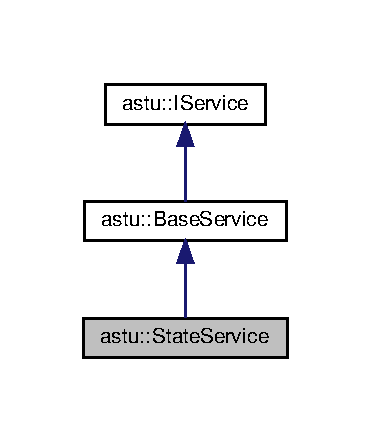
\includegraphics[width=196pt]{classastu_1_1StateService__inherit__graph}
\end{center}
\end{figure}


Collaboration diagram for astu\+:\+:State\+Service\+:\nopagebreak
\begin{figure}[H]
\begin{center}
\leavevmode
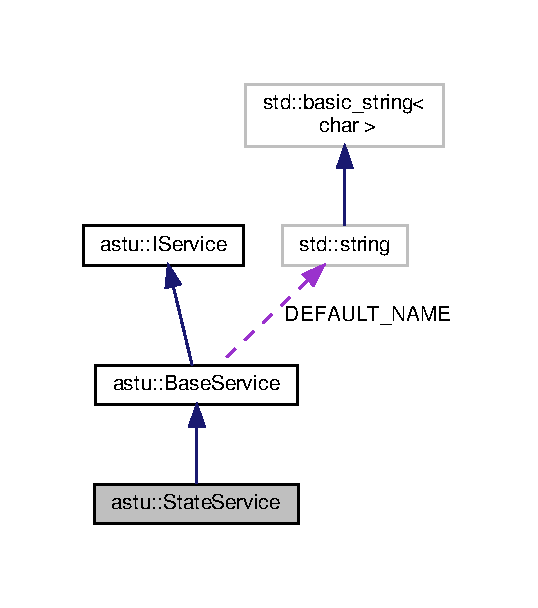
\includegraphics[width=310pt]{classastu_1_1StateService__coll__graph}
\end{center}
\end{figure}
\subsection*{Public Member Functions}
\begin{DoxyCompactItemize}
\item 
\hyperlink{classastu_1_1StateService_ae8be300ce5fd92351d52fc7162ce9793}{State\+Service} ()
\item 
\hyperlink{classastu_1_1StateService_a27bbe3ef0f9a4600c559ca9f6def3f5f}{$\sim$\+State\+Service} ()
\item 
void \hyperlink{classastu_1_1StateService_a5b6125be259b52bf9f3e80453def9e21}{Add\+Service} (const std\+::string \&state, std\+::shared\+\_\+ptr$<$ \hyperlink{classastu_1_1IService}{I\+Service} $>$ srv)
\item 
bool \hyperlink{classastu_1_1StateService_a611255de384fd0e53fccf30cb53662b6}{Has\+Service} (const std\+::string \&state, std\+::shared\+\_\+ptr$<$ \hyperlink{classastu_1_1IService}{I\+Service} $>$ srv) const
\item 
bool \hyperlink{classastu_1_1StateService_adfd94f9b5d622131a1fdcc4dcf5ef51d}{Has\+State} (const std\+::string \&state) const
\item 
void \hyperlink{classastu_1_1StateService_ae1916f97f8f386b6f4ac42d58c0ae97f}{Create\+State} (const std\+::string \&state)
\item 
void \hyperlink{classastu_1_1StateService_a3396bad71a626dd749295375759015d3}{Switch\+State} (const std\+::string \&state)
\item 
const std\+::string \& \hyperlink{classastu_1_1StateService_ac643aebb1bfe9880db1bac7533e0ec75}{Get\+Current\+State} () const
\end{DoxyCompactItemize}
\subsection*{Protected Member Functions}
\begin{DoxyCompactItemize}
\item 
virtual void \hyperlink{classastu_1_1StateService_a06419feca958b72db99dde6eda301f86}{On\+Startup} () override
\item 
virtual void \hyperlink{classastu_1_1StateService_ad8fa5b6d52bd795ebba450f119540d87}{On\+Shutdown} () override
\end{DoxyCompactItemize}
\subsection*{Additional Inherited Members}


\subsection{Detailed Description}
The state service manages a set of states.

Each of these states contains a list of services that are added to the active services when the state is activated. As soon as the state is changed, the services of the current state are removed and those of the new state are added accordingly. 

\subsection{Constructor \& Destructor Documentation}
\mbox{\Hypertarget{classastu_1_1StateService_ae8be300ce5fd92351d52fc7162ce9793}\label{classastu_1_1StateService_ae8be300ce5fd92351d52fc7162ce9793}} 
\index{astu\+::\+State\+Service@{astu\+::\+State\+Service}!State\+Service@{State\+Service}}
\index{State\+Service@{State\+Service}!astu\+::\+State\+Service@{astu\+::\+State\+Service}}
\subsubsection{\texorpdfstring{State\+Service()}{StateService()}}
{\footnotesize\ttfamily astu\+::\+State\+Service\+::\+State\+Service (\begin{DoxyParamCaption}{ }\end{DoxyParamCaption})}

Constructor. \mbox{\Hypertarget{classastu_1_1StateService_a27bbe3ef0f9a4600c559ca9f6def3f5f}\label{classastu_1_1StateService_a27bbe3ef0f9a4600c559ca9f6def3f5f}} 
\index{astu\+::\+State\+Service@{astu\+::\+State\+Service}!````~State\+Service@{$\sim$\+State\+Service}}
\index{````~State\+Service@{$\sim$\+State\+Service}!astu\+::\+State\+Service@{astu\+::\+State\+Service}}
\subsubsection{\texorpdfstring{$\sim$\+State\+Service()}{~StateService()}}
{\footnotesize\ttfamily astu\+::\+State\+Service\+::$\sim$\+State\+Service (\begin{DoxyParamCaption}{ }\end{DoxyParamCaption})\hspace{0.3cm}{\ttfamily [inline]}}

Virtual destructor. 

\subsection{Member Function Documentation}
\mbox{\Hypertarget{classastu_1_1StateService_a5b6125be259b52bf9f3e80453def9e21}\label{classastu_1_1StateService_a5b6125be259b52bf9f3e80453def9e21}} 
\index{astu\+::\+State\+Service@{astu\+::\+State\+Service}!Add\+Service@{Add\+Service}}
\index{Add\+Service@{Add\+Service}!astu\+::\+State\+Service@{astu\+::\+State\+Service}}
\subsubsection{\texorpdfstring{Add\+Service()}{AddService()}}
{\footnotesize\ttfamily void astu\+::\+State\+Service\+::\+Add\+Service (\begin{DoxyParamCaption}\item[{const std\+::string \&}]{state,  }\item[{std\+::shared\+\_\+ptr$<$ \hyperlink{classastu_1_1IService}{I\+Service} $>$}]{srv }\end{DoxyParamCaption})}

Adds a service to a state.

If the state does not yet exist, it will be created.


\begin{DoxyParams}{Parameters}
{\em state} & the name of the state \\
\hline
{\em srv} & the service to add \\
\hline
\end{DoxyParams}

\begin{DoxyExceptions}{Exceptions}
{\em std\+::logic\+\_\+error} & in case the service has already beed added \\
\hline
\end{DoxyExceptions}
\mbox{\Hypertarget{classastu_1_1StateService_ae1916f97f8f386b6f4ac42d58c0ae97f}\label{classastu_1_1StateService_ae1916f97f8f386b6f4ac42d58c0ae97f}} 
\index{astu\+::\+State\+Service@{astu\+::\+State\+Service}!Create\+State@{Create\+State}}
\index{Create\+State@{Create\+State}!astu\+::\+State\+Service@{astu\+::\+State\+Service}}
\subsubsection{\texorpdfstring{Create\+State()}{CreateState()}}
{\footnotesize\ttfamily void astu\+::\+State\+Service\+::\+Create\+State (\begin{DoxyParamCaption}\item[{const std\+::string \&}]{state }\end{DoxyParamCaption})}

Creates a new empty state.


\begin{DoxyParams}{Parameters}
{\em state} & the name of the state \\
\hline
\end{DoxyParams}

\begin{DoxyExceptions}{Exceptions}
{\em std\+::logic\+\_\+error} & in case the state name is ambiguous \\
\hline
\end{DoxyExceptions}
\mbox{\Hypertarget{classastu_1_1StateService_ac643aebb1bfe9880db1bac7533e0ec75}\label{classastu_1_1StateService_ac643aebb1bfe9880db1bac7533e0ec75}} 
\index{astu\+::\+State\+Service@{astu\+::\+State\+Service}!Get\+Current\+State@{Get\+Current\+State}}
\index{Get\+Current\+State@{Get\+Current\+State}!astu\+::\+State\+Service@{astu\+::\+State\+Service}}
\subsubsection{\texorpdfstring{Get\+Current\+State()}{GetCurrentState()}}
{\footnotesize\ttfamily const std\+::string\& astu\+::\+State\+Service\+::\+Get\+Current\+State (\begin{DoxyParamCaption}{ }\end{DoxyParamCaption}) const}

Returns the name of the current state.

\begin{DoxyReturn}{Returns}
the current state name 
\end{DoxyReturn}
\mbox{\Hypertarget{classastu_1_1StateService_a611255de384fd0e53fccf30cb53662b6}\label{classastu_1_1StateService_a611255de384fd0e53fccf30cb53662b6}} 
\index{astu\+::\+State\+Service@{astu\+::\+State\+Service}!Has\+Service@{Has\+Service}}
\index{Has\+Service@{Has\+Service}!astu\+::\+State\+Service@{astu\+::\+State\+Service}}
\subsubsection{\texorpdfstring{Has\+Service()}{HasService()}}
{\footnotesize\ttfamily bool astu\+::\+State\+Service\+::\+Has\+Service (\begin{DoxyParamCaption}\item[{const std\+::string \&}]{state,  }\item[{std\+::shared\+\_\+ptr$<$ \hyperlink{classastu_1_1IService}{I\+Service} $>$}]{srv }\end{DoxyParamCaption}) const}

Tests whether a service has already been added to a state.


\begin{DoxyParams}{Parameters}
{\em state} & the name of the state \\
\hline
{\em srv} & the service to add \\
\hline
\end{DoxyParams}
\begin{DoxyReturn}{Returns}
{\ttfamily true} if the service has already been added 
\end{DoxyReturn}
\mbox{\Hypertarget{classastu_1_1StateService_adfd94f9b5d622131a1fdcc4dcf5ef51d}\label{classastu_1_1StateService_adfd94f9b5d622131a1fdcc4dcf5ef51d}} 
\index{astu\+::\+State\+Service@{astu\+::\+State\+Service}!Has\+State@{Has\+State}}
\index{Has\+State@{Has\+State}!astu\+::\+State\+Service@{astu\+::\+State\+Service}}
\subsubsection{\texorpdfstring{Has\+State()}{HasState()}}
{\footnotesize\ttfamily bool astu\+::\+State\+Service\+::\+Has\+State (\begin{DoxyParamCaption}\item[{const std\+::string \&}]{state }\end{DoxyParamCaption}) const}

Tests whether a state exists.


\begin{DoxyParams}{Parameters}
{\em state} & the name of the state \\
\hline
\end{DoxyParams}
\begin{DoxyReturn}{Returns}
{\ttfamily true} if the state exists 
\end{DoxyReturn}
\mbox{\Hypertarget{classastu_1_1StateService_ad8fa5b6d52bd795ebba450f119540d87}\label{classastu_1_1StateService_ad8fa5b6d52bd795ebba450f119540d87}} 
\index{astu\+::\+State\+Service@{astu\+::\+State\+Service}!On\+Shutdown@{On\+Shutdown}}
\index{On\+Shutdown@{On\+Shutdown}!astu\+::\+State\+Service@{astu\+::\+State\+Service}}
\subsubsection{\texorpdfstring{On\+Shutdown()}{OnShutdown()}}
{\footnotesize\ttfamily virtual void astu\+::\+State\+Service\+::\+On\+Shutdown (\begin{DoxyParamCaption}{ }\end{DoxyParamCaption})\hspace{0.3cm}{\ttfamily [override]}, {\ttfamily [protected]}, {\ttfamily [virtual]}}

Called by this base class on shutdown.

Derived classes should override this method rather than {\ttfamily \hyperlink{classastu_1_1BaseService_a7095888244052db294d58738c0d187fb}{Shutdown()}}. The {\ttfamily \hyperlink{classastu_1_1BaseService_a7095888244052db294d58738c0d187fb}{Shutdown()}} method is maintaining the running-\/state of this service. 

Reimplemented from \hyperlink{classastu_1_1BaseService_aeb5003f7c5efe5412725ac4c66942d03}{astu\+::\+Base\+Service}.

\mbox{\Hypertarget{classastu_1_1StateService_a06419feca958b72db99dde6eda301f86}\label{classastu_1_1StateService_a06419feca958b72db99dde6eda301f86}} 
\index{astu\+::\+State\+Service@{astu\+::\+State\+Service}!On\+Startup@{On\+Startup}}
\index{On\+Startup@{On\+Startup}!astu\+::\+State\+Service@{astu\+::\+State\+Service}}
\subsubsection{\texorpdfstring{On\+Startup()}{OnStartup()}}
{\footnotesize\ttfamily virtual void astu\+::\+State\+Service\+::\+On\+Startup (\begin{DoxyParamCaption}{ }\end{DoxyParamCaption})\hspace{0.3cm}{\ttfamily [override]}, {\ttfamily [protected]}, {\ttfamily [virtual]}}

Called by this base class on startup.

Derived classes should override this method rather than {\ttfamily \hyperlink{classastu_1_1BaseService_a59dade033dcb44dd32155c526a3a58e2}{Startup()}}. The {\ttfamily \hyperlink{classastu_1_1BaseService_a59dade033dcb44dd32155c526a3a58e2}{Startup()}} method is maintaining the running-\/state of this service. 

Reimplemented from \hyperlink{classastu_1_1BaseService_ac8710cd2d6dcc990db65e7c8ccfbc5ff}{astu\+::\+Base\+Service}.

\mbox{\Hypertarget{classastu_1_1StateService_a3396bad71a626dd749295375759015d3}\label{classastu_1_1StateService_a3396bad71a626dd749295375759015d3}} 
\index{astu\+::\+State\+Service@{astu\+::\+State\+Service}!Switch\+State@{Switch\+State}}
\index{Switch\+State@{Switch\+State}!astu\+::\+State\+Service@{astu\+::\+State\+Service}}
\subsubsection{\texorpdfstring{Switch\+State()}{SwitchState()}}
{\footnotesize\ttfamily void astu\+::\+State\+Service\+::\+Switch\+State (\begin{DoxyParamCaption}\item[{const std\+::string \&}]{state }\end{DoxyParamCaption})}

Switches to a certain state.


\begin{DoxyParams}{Parameters}
{\em state} & the name of the state to switch \\
\hline
\end{DoxyParams}

\begin{DoxyExceptions}{Exceptions}
{\em std\+::logic\+\_\+error} & in case the state is unknown \\
\hline
\end{DoxyExceptions}


The documentation for this class was generated from the following file\+:\begin{DoxyCompactItemize}
\item 
include/State\+Service.\+h\end{DoxyCompactItemize}

\hypertarget{classastu_1_1UpdatableBaseService}{}\section{astu\+:\+:Updatable\+Base\+Service Class Reference}
\label{classastu_1_1UpdatableBaseService}\index{astu\+::\+Updatable\+Base\+Service@{astu\+::\+Updatable\+Base\+Service}}


{\ttfamily \#include $<$Update\+Service.\+h$>$}



Inheritance diagram for astu\+:\+:Updatable\+Base\+Service\+:\nopagebreak
\begin{figure}[H]
\begin{center}
\leavevmode
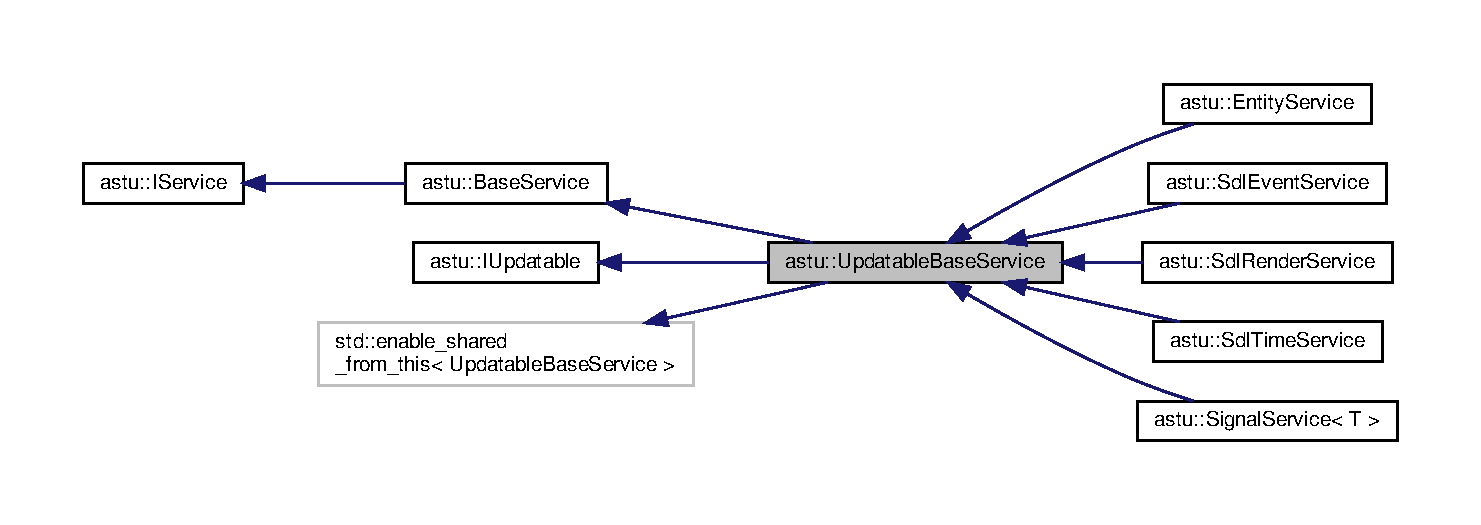
\includegraphics[width=350pt]{classastu_1_1UpdatableBaseService__inherit__graph}
\end{center}
\end{figure}


Collaboration diagram for astu\+:\+:Updatable\+Base\+Service\+:\nopagebreak
\begin{figure}[H]
\begin{center}
\leavevmode
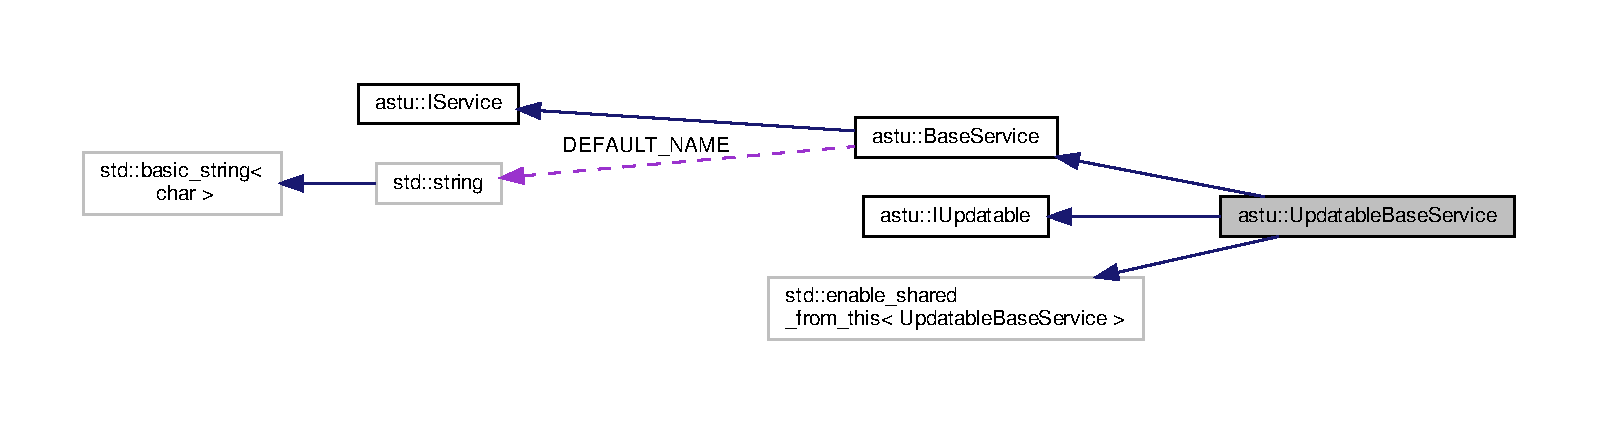
\includegraphics[width=350pt]{classastu_1_1UpdatableBaseService__coll__graph}
\end{center}
\end{figure}
\subsection*{Public Member Functions}
\begin{DoxyCompactItemize}
\item 
\hyperlink{classastu_1_1UpdatableBaseService_affb07c2699a08b42eb5b8ca96ed681c0}{Updatable\+Base\+Service} (const std\+::string \&name=\hyperlink{classastu_1_1BaseService_a9483b26ad631bd14646ef2d2170cd828}{D\+E\+F\+A\+U\+L\+T\+\_\+\+N\+A\+ME}, int priority=0)
\item 
virtual void \hyperlink{classastu_1_1UpdatableBaseService_a47e3725f717cee3cd8983f485b2a0243}{Startup} () override
\item 
virtual void \hyperlink{classastu_1_1UpdatableBaseService_a7ad7e0201007878b6014361dd5ba82f9}{Shutdown} () override
\item 
virtual int \hyperlink{classastu_1_1UpdatableBaseService_a22a9824510d94fa97efb962ae38be945}{Get\+Update\+Priority} () const override
\end{DoxyCompactItemize}
\subsection*{Additional Inherited Members}


\subsection{Detailed Description}
Base class for services whitch require an update. 

\subsection{Constructor \& Destructor Documentation}
\mbox{\Hypertarget{classastu_1_1UpdatableBaseService_affb07c2699a08b42eb5b8ca96ed681c0}\label{classastu_1_1UpdatableBaseService_affb07c2699a08b42eb5b8ca96ed681c0}} 
\index{astu\+::\+Updatable\+Base\+Service@{astu\+::\+Updatable\+Base\+Service}!Updatable\+Base\+Service@{Updatable\+Base\+Service}}
\index{Updatable\+Base\+Service@{Updatable\+Base\+Service}!astu\+::\+Updatable\+Base\+Service@{astu\+::\+Updatable\+Base\+Service}}
\subsubsection{\texorpdfstring{Updatable\+Base\+Service()}{UpdatableBaseService()}}
{\footnotesize\ttfamily astu\+::\+Updatable\+Base\+Service\+::\+Updatable\+Base\+Service (\begin{DoxyParamCaption}\item[{const std\+::string \&}]{name = {\ttfamily \hyperlink{classastu_1_1BaseService_a9483b26ad631bd14646ef2d2170cd828}{D\+E\+F\+A\+U\+L\+T\+\_\+\+N\+A\+ME}},  }\item[{int}]{priority = {\ttfamily 0} }\end{DoxyParamCaption})}

Constructor.


\begin{DoxyParams}{Parameters}
{\em name} & the name of this service \\
\hline
{\em priority} & the update priority of this service \\
\hline
\end{DoxyParams}


\subsection{Member Function Documentation}
\mbox{\Hypertarget{classastu_1_1UpdatableBaseService_a22a9824510d94fa97efb962ae38be945}\label{classastu_1_1UpdatableBaseService_a22a9824510d94fa97efb962ae38be945}} 
\index{astu\+::\+Updatable\+Base\+Service@{astu\+::\+Updatable\+Base\+Service}!Get\+Update\+Priority@{Get\+Update\+Priority}}
\index{Get\+Update\+Priority@{Get\+Update\+Priority}!astu\+::\+Updatable\+Base\+Service@{astu\+::\+Updatable\+Base\+Service}}
\subsubsection{\texorpdfstring{Get\+Update\+Priority()}{GetUpdatePriority()}}
{\footnotesize\ttfamily virtual int astu\+::\+Updatable\+Base\+Service\+::\+Get\+Update\+Priority (\begin{DoxyParamCaption}{ }\end{DoxyParamCaption}) const\hspace{0.3cm}{\ttfamily [override]}, {\ttfamily [virtual]}}

Returns the update priority.

Updatables with lower priorities get updated before updatables with higher priorities.

\begin{DoxyReturn}{Returns}
the update priority 
\end{DoxyReturn}


Implements \hyperlink{classastu_1_1IUpdatable_a1bf76b0fce2360b8ade25ef9ae9e3065}{astu\+::\+I\+Updatable}.

\mbox{\Hypertarget{classastu_1_1UpdatableBaseService_a7ad7e0201007878b6014361dd5ba82f9}\label{classastu_1_1UpdatableBaseService_a7ad7e0201007878b6014361dd5ba82f9}} 
\index{astu\+::\+Updatable\+Base\+Service@{astu\+::\+Updatable\+Base\+Service}!Shutdown@{Shutdown}}
\index{Shutdown@{Shutdown}!astu\+::\+Updatable\+Base\+Service@{astu\+::\+Updatable\+Base\+Service}}
\subsubsection{\texorpdfstring{Shutdown()}{Shutdown()}}
{\footnotesize\ttfamily virtual void astu\+::\+Updatable\+Base\+Service\+::\+Shutdown (\begin{DoxyParamCaption}{ }\end{DoxyParamCaption})\hspace{0.3cm}{\ttfamily [override]}, {\ttfamily [virtual]}}

Stops this service.

In case this service is currently not running, calling this method has no effect. 

Reimplemented from \hyperlink{classastu_1_1BaseService_a7095888244052db294d58738c0d187fb}{astu\+::\+Base\+Service}.

\mbox{\Hypertarget{classastu_1_1UpdatableBaseService_a47e3725f717cee3cd8983f485b2a0243}\label{classastu_1_1UpdatableBaseService_a47e3725f717cee3cd8983f485b2a0243}} 
\index{astu\+::\+Updatable\+Base\+Service@{astu\+::\+Updatable\+Base\+Service}!Startup@{Startup}}
\index{Startup@{Startup}!astu\+::\+Updatable\+Base\+Service@{astu\+::\+Updatable\+Base\+Service}}
\subsubsection{\texorpdfstring{Startup()}{Startup()}}
{\footnotesize\ttfamily virtual void astu\+::\+Updatable\+Base\+Service\+::\+Startup (\begin{DoxyParamCaption}{ }\end{DoxyParamCaption})\hspace{0.3cm}{\ttfamily [override]}, {\ttfamily [virtual]}}

Starts this service.


\begin{DoxyExceptions}{Exceptions}
{\em std\+::logic\+\_\+error} & in case this service is already running \\
\hline
\end{DoxyExceptions}


Reimplemented from \hyperlink{classastu_1_1BaseService_a59dade033dcb44dd32155c526a3a58e2}{astu\+::\+Base\+Service}.



The documentation for this class was generated from the following file\+:\begin{DoxyCompactItemize}
\item 
include/Update\+Service.\+h\end{DoxyCompactItemize}

\hypertarget{classastu_1_1UpdateService}{}\section{astu\+:\+:Update\+Service Class Reference}
\label{classastu_1_1UpdateService}\index{astu\+::\+Update\+Service@{astu\+::\+Update\+Service}}


{\ttfamily \#include $<$Update\+Service.\+h$>$}



Inheritance diagram for astu\+:\+:Update\+Service\+:\nopagebreak
\begin{figure}[H]
\begin{center}
\leavevmode
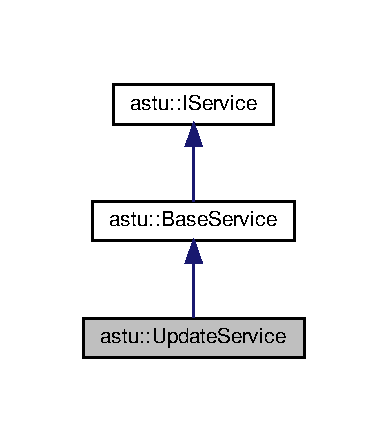
\includegraphics[width=186pt]{classastu_1_1UpdateService__inherit__graph}
\end{center}
\end{figure}


Collaboration diagram for astu\+:\+:Update\+Service\+:\nopagebreak
\begin{figure}[H]
\begin{center}
\leavevmode
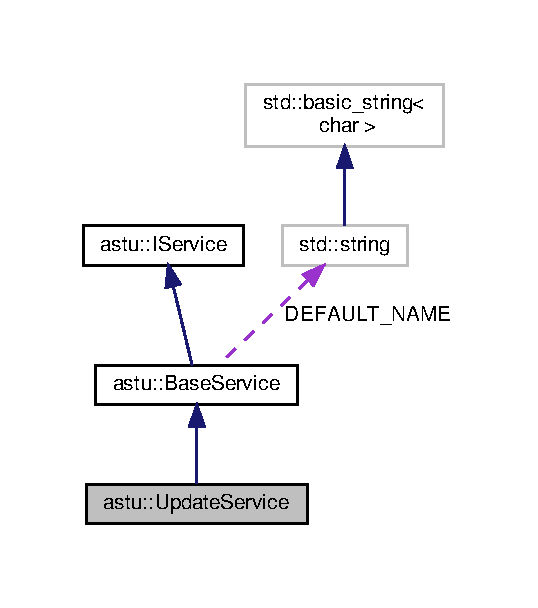
\includegraphics[width=258pt]{classastu_1_1UpdateService__coll__graph}
\end{center}
\end{figure}
\subsection*{Public Member Functions}
\begin{DoxyCompactItemize}
\item 
\hyperlink{classastu_1_1UpdateService_ae4d88fb4772931e35f7c46b7d756b4c8}{Update\+Service} ()
\item 
void \hyperlink{classastu_1_1UpdateService_a83ff161f4280681a50b728e2ac157cf6}{Add\+Updatable} (std\+::shared\+\_\+ptr$<$ \hyperlink{classastu_1_1IUpdatable}{I\+Updatable} $>$ updatable)
\item 
void \hyperlink{classastu_1_1UpdateService_a04911354dbfbf3849fafda10209710b6}{Remove\+Updatable} (std\+::shared\+\_\+ptr$<$ \hyperlink{classastu_1_1IUpdatable}{I\+Updatable} $>$ updatable)
\item 
bool \hyperlink{classastu_1_1UpdateService_aaffeece0ab9fd8fff1020763cd72de13}{Has\+Updatable} (std\+::shared\+\_\+ptr$<$ \hyperlink{classastu_1_1IUpdatable}{I\+Updatable} $>$ updatable)
\item 
\mbox{\Hypertarget{classastu_1_1UpdateService_a9ee615ce365e1910446a2646b0a2ad9a}\label{classastu_1_1UpdateService_a9ee615ce365e1910446a2646b0a2ad9a}} 
void {\bfseries Update\+All} ()
\end{DoxyCompactItemize}
\subsection*{Additional Inherited Members}


\subsection{Detailed Description}
This service manages and updates {\ttfamily Updatables}.

To update the {\ttfamily Updatables}, this service\textquotesingle{}s method {\ttfamily Update\+All} must be called within the simulation respectively game loop. 

\subsection{Constructor \& Destructor Documentation}
\mbox{\Hypertarget{classastu_1_1UpdateService_ae4d88fb4772931e35f7c46b7d756b4c8}\label{classastu_1_1UpdateService_ae4d88fb4772931e35f7c46b7d756b4c8}} 
\index{astu\+::\+Update\+Service@{astu\+::\+Update\+Service}!Update\+Service@{Update\+Service}}
\index{Update\+Service@{Update\+Service}!astu\+::\+Update\+Service@{astu\+::\+Update\+Service}}
\subsubsection{\texorpdfstring{Update\+Service()}{UpdateService()}}
{\footnotesize\ttfamily astu\+::\+Update\+Service\+::\+Update\+Service (\begin{DoxyParamCaption}{ }\end{DoxyParamCaption})}

Constructor. 

\subsection{Member Function Documentation}
\mbox{\Hypertarget{classastu_1_1UpdateService_a83ff161f4280681a50b728e2ac157cf6}\label{classastu_1_1UpdateService_a83ff161f4280681a50b728e2ac157cf6}} 
\index{astu\+::\+Update\+Service@{astu\+::\+Update\+Service}!Add\+Updatable@{Add\+Updatable}}
\index{Add\+Updatable@{Add\+Updatable}!astu\+::\+Update\+Service@{astu\+::\+Update\+Service}}
\subsubsection{\texorpdfstring{Add\+Updatable()}{AddUpdatable()}}
{\footnotesize\ttfamily void astu\+::\+Update\+Service\+::\+Add\+Updatable (\begin{DoxyParamCaption}\item[{std\+::shared\+\_\+ptr$<$ \hyperlink{classastu_1_1IUpdatable}{I\+Updatable} $>$}]{updatable }\end{DoxyParamCaption})}

Adds an updatable.


\begin{DoxyParams}{Parameters}
{\em updatable} & the updatable to be added \\
\hline
\end{DoxyParams}
\mbox{\Hypertarget{classastu_1_1UpdateService_aaffeece0ab9fd8fff1020763cd72de13}\label{classastu_1_1UpdateService_aaffeece0ab9fd8fff1020763cd72de13}} 
\index{astu\+::\+Update\+Service@{astu\+::\+Update\+Service}!Has\+Updatable@{Has\+Updatable}}
\index{Has\+Updatable@{Has\+Updatable}!astu\+::\+Update\+Service@{astu\+::\+Update\+Service}}
\subsubsection{\texorpdfstring{Has\+Updatable()}{HasUpdatable()}}
{\footnotesize\ttfamily bool astu\+::\+Update\+Service\+::\+Has\+Updatable (\begin{DoxyParamCaption}\item[{std\+::shared\+\_\+ptr$<$ \hyperlink{classastu_1_1IUpdatable}{I\+Updatable} $>$}]{updatable }\end{DoxyParamCaption})}

Tests whether a specific updatablel has already been added.


\begin{DoxyParams}{Parameters}
{\em updatable} & the updatable to be tested \\
\hline
\end{DoxyParams}
\begin{DoxyReturn}{Returns}
{\ttfamily true} if the updatale has already beed added 
\end{DoxyReturn}
\mbox{\Hypertarget{classastu_1_1UpdateService_a04911354dbfbf3849fafda10209710b6}\label{classastu_1_1UpdateService_a04911354dbfbf3849fafda10209710b6}} 
\index{astu\+::\+Update\+Service@{astu\+::\+Update\+Service}!Remove\+Updatable@{Remove\+Updatable}}
\index{Remove\+Updatable@{Remove\+Updatable}!astu\+::\+Update\+Service@{astu\+::\+Update\+Service}}
\subsubsection{\texorpdfstring{Remove\+Updatable()}{RemoveUpdatable()}}
{\footnotesize\ttfamily void astu\+::\+Update\+Service\+::\+Remove\+Updatable (\begin{DoxyParamCaption}\item[{std\+::shared\+\_\+ptr$<$ \hyperlink{classastu_1_1IUpdatable}{I\+Updatable} $>$}]{updatable }\end{DoxyParamCaption})}

Removes an updatable.


\begin{DoxyParams}{Parameters}
{\em updatable} & the updatable to be removed \\
\hline
\end{DoxyParams}


The documentation for this class was generated from the following file\+:\begin{DoxyCompactItemize}
\item 
include/Update\+Service.\+h\end{DoxyCompactItemize}

\chapter{File Documentation}
\hypertarget{AstEcs_8h}{}\section{include/\+Ast\+Ecs.h File Reference}
\label{AstEcs_8h}\index{include/\+Ast\+Ecs.\+h@{include/\+Ast\+Ecs.\+h}}


This file defines public functions, templates and classes offered by the entity component system (E\+CS) of A\+ST utilities.  


{\ttfamily \#include \char`\"{}Entity\+Service.\+h\char`\"{}}\newline
{\ttfamily \#include \char`\"{}Iterating\+Entity\+System.\+h\char`\"{}}\newline
Include dependency graph for Ast\+Ecs.\+h\+:\nopagebreak
\begin{figure}[H]
\begin{center}
\leavevmode
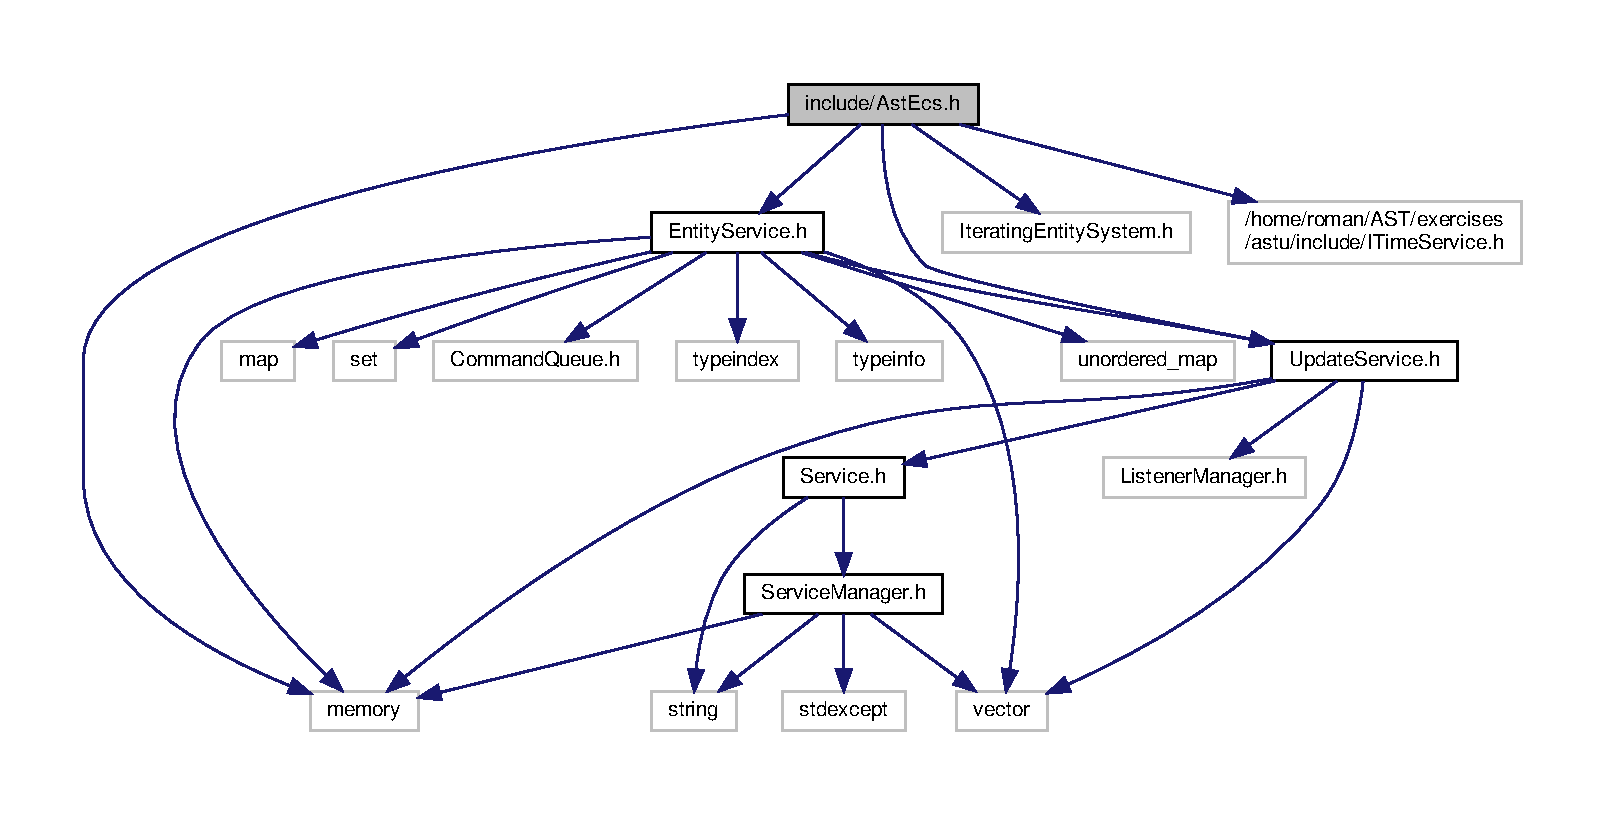
\includegraphics[width=350pt]{AstEcs_8h__incl}
\end{center}
\end{figure}


\subsection{Detailed Description}
This file defines public functions, templates and classes offered by the entity component system (E\+CS) of A\+ST utilities. 


\hypertarget{AstGraphics_8h}{}\section{include/\+Ast\+Graphics.h File Reference}
\label{AstGraphics_8h}\index{include/\+Ast\+Graphics.\+h@{include/\+Ast\+Graphics.\+h}}


This file defines public functions offered by the graphics module of A\+ST utilities.  


{\ttfamily \#include $<$string$>$}\newline
{\ttfamily \#include $<$memory$>$}\newline
{\ttfamily \#include \char`\"{}Color.\+h\char`\"{}}\newline
{\ttfamily \#include \char`\"{}Color\+Hsv.\+h\char`\"{}}\newline
{\ttfamily \#include \char`\"{}Vector2.\+h\char`\"{}}\newline
{\ttfamily \#include \char`\"{}Palette.\+h\char`\"{}}\newline
{\ttfamily \#include \char`\"{}Image.\+h\char`\"{}}\newline
{\ttfamily \#include \char`\"{}Image\+Renderer.\+h\char`\"{}}\newline
{\ttfamily \#include \char`\"{}Turtle.\+h\char`\"{}}\newline
Include dependency graph for Ast\+Graphics.\+h\+:\nopagebreak
\begin{figure}[H]
\begin{center}
\leavevmode
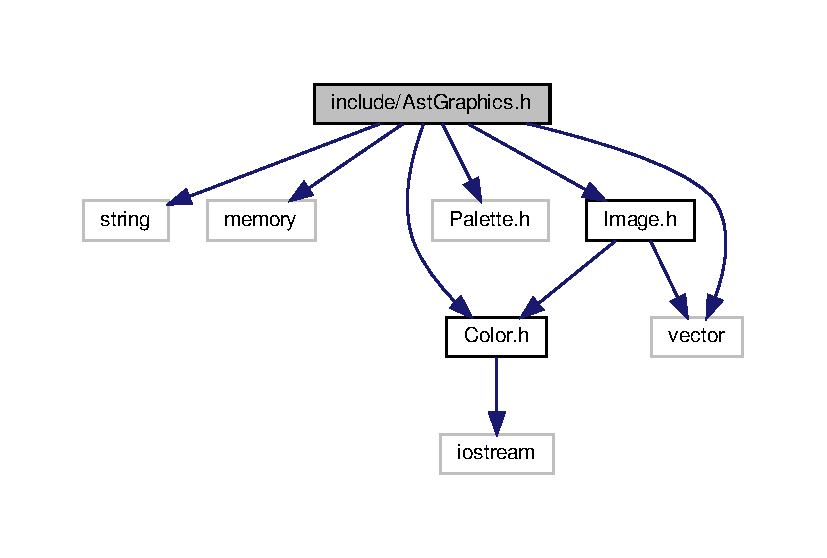
\includegraphics[width=350pt]{AstGraphics_8h__incl}
\end{center}
\end{figure}
\subsection*{Functions}
\begin{DoxyCompactItemize}
\item 
void \hyperlink{group__gfx__group_gaca5f9cb8047c60049300242c20d30cd6}{astu\+::\+Store\+Image} (const Image \&image, const std\+::string \&filename)
\item 
std\+::unique\+\_\+ptr$<$ Image $>$ \hyperlink{group__gfx__group_ga46ac561eac42d4ace785797db8bc89a0}{astu\+::\+Load\+Image} (const std\+::string \&filename)
\end{DoxyCompactItemize}


\subsection{Detailed Description}
This file defines public functions offered by the graphics module of A\+ST utilities. 


\hypertarget{AstInput_8h}{}\section{include/\+Ast\+Input.h File Reference}
\label{AstInput_8h}\index{include/\+Ast\+Input.\+h@{include/\+Ast\+Input.\+h}}


This file defines public functions, templates and classes provided by input module.  


{\ttfamily \#include \char`\"{}Mouse.\+h\char`\"{}}\newline
{\ttfamily \#include \char`\"{}Events.\+h\char`\"{}}\newline
Include dependency graph for Ast\+Input.\+h\+:\nopagebreak
\begin{figure}[H]
\begin{center}
\leavevmode
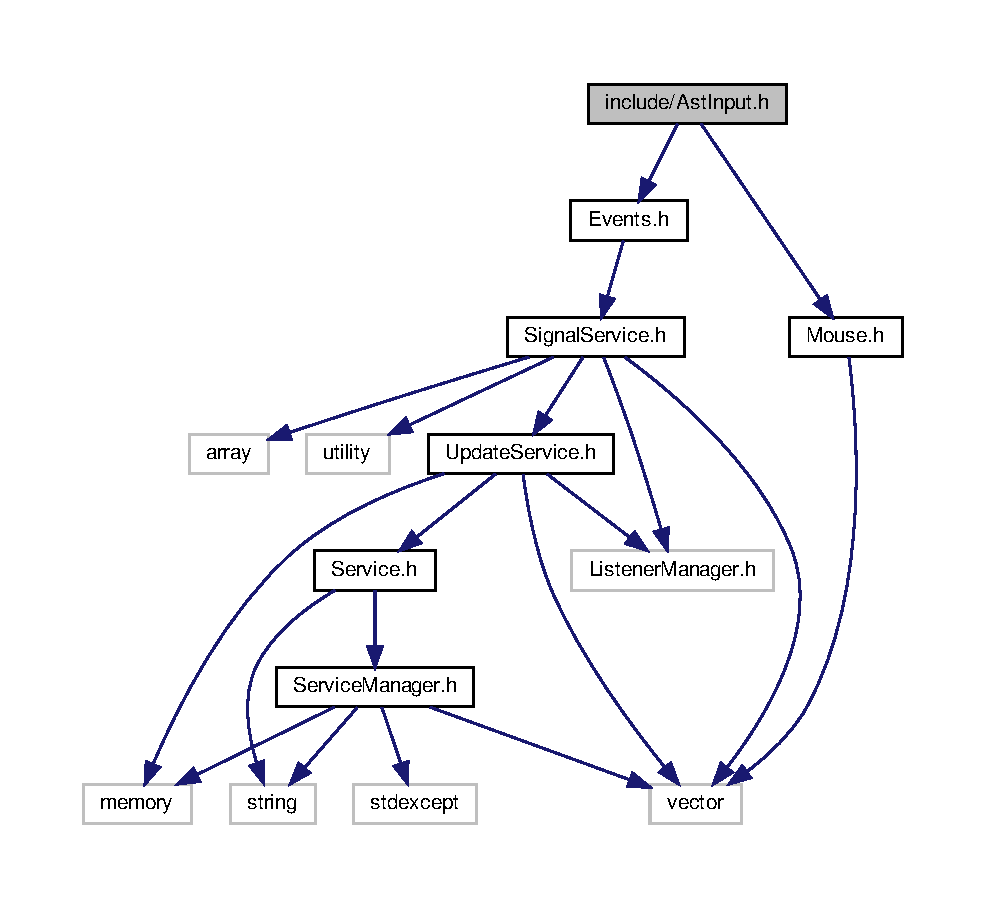
\includegraphics[width=350pt]{AstInput_8h__incl}
\end{center}
\end{figure}


\subsection{Detailed Description}
This file defines public functions, templates and classes provided by input module. 


\hypertarget{AstIO_8h}{}\section{include/\+Ast\+IO.h File Reference}
\label{AstIO_8h}\index{include/\+Ast\+I\+O.\+h@{include/\+Ast\+I\+O.\+h}}


This file defines public functions offered by the I/O module of A\+ST utilities.  


{\ttfamily \#include $<$string$>$}\newline
Include dependency graph for Ast\+I\+O.\+h\+:\nopagebreak
\begin{figure}[H]
\begin{center}
\leavevmode
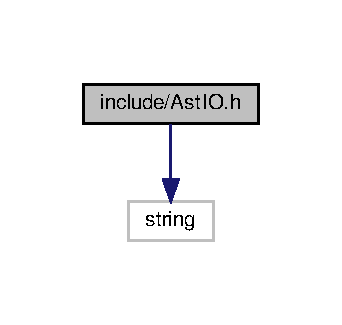
\includegraphics[width=164pt]{AstIO_8h__incl}
\end{center}
\end{figure}
\subsection*{Functions}
\begin{DoxyCompactItemize}
\item 
void \hyperlink{AstIO_8h_a7cc89ae306750b9cfebac64bb5e9181c}{astu\+::\+Skip\+Line} ()
\item 
std\+::string \hyperlink{AstIO_8h_ac80dcbf4d76b7e0f3b4e44617e005608}{astu\+::\+Query\+String} (const std\+::string \&text)
\item 
int \hyperlink{AstIO_8h_ad54c0019fb3e7671e9b32db9cb3d7ebe}{astu\+::\+Query\+Int} (const std\+::string \&text)
\end{DoxyCompactItemize}


\subsection{Detailed Description}
This file defines public functions offered by the I/O module of A\+ST utilities. 



\subsection{Function Documentation}
\mbox{\Hypertarget{AstIO_8h_file_ad54c0019fb3e7671e9b32db9cb3d7ebe}\label{AstIO_8h_file_ad54c0019fb3e7671e9b32db9cb3d7ebe}} 
\index{Ast\+I\+O.\+h@{Ast\+I\+O.\+h}!Query\+Int@{Query\+Int}}
\index{Query\+Int@{Query\+Int}!Ast\+I\+O.\+h@{Ast\+I\+O.\+h}}
\subsubsection{\texorpdfstring{Query\+Int()}{QueryInt()}}
{\footnotesize\ttfamily int astu\+::\+Query\+Int (\begin{DoxyParamCaption}\item[{const std\+::string \&}]{text }\end{DoxyParamCaption})}

Queries an integer value from the standard input stream.

This function ensures that no additional characters entered by the user remain in the input stream.


\begin{DoxyParams}{Parameters}
{\em text} & preceding text printed before the use input is collected \\
\hline
\end{DoxyParams}
\begin{DoxyReturn}{Returns}
the integer value entered by the user 
\end{DoxyReturn}
\mbox{\Hypertarget{AstIO_8h_file_ac80dcbf4d76b7e0f3b4e44617e005608}\label{AstIO_8h_file_ac80dcbf4d76b7e0f3b4e44617e005608}} 
\index{Ast\+I\+O.\+h@{Ast\+I\+O.\+h}!Query\+String@{Query\+String}}
\index{Query\+String@{Query\+String}!Ast\+I\+O.\+h@{Ast\+I\+O.\+h}}
\subsubsection{\texorpdfstring{Query\+String()}{QueryString()}}
{\footnotesize\ttfamily std\+::string astu\+::\+Query\+String (\begin{DoxyParamCaption}\item[{const std\+::string \&}]{text }\end{DoxyParamCaption})}

Queries a string from the standard input stream.


\begin{DoxyParams}{Parameters}
{\em text} & preceding text printed before the use input is collected \\
\hline
\end{DoxyParams}
\begin{DoxyReturn}{Returns}
the string entered by the user 
\end{DoxyReturn}
\mbox{\Hypertarget{AstIO_8h_file_a7cc89ae306750b9cfebac64bb5e9181c}\label{AstIO_8h_file_a7cc89ae306750b9cfebac64bb5e9181c}} 
\index{Ast\+I\+O.\+h@{Ast\+I\+O.\+h}!Skip\+Line@{Skip\+Line}}
\index{Skip\+Line@{Skip\+Line}!Ast\+I\+O.\+h@{Ast\+I\+O.\+h}}
\subsubsection{\texorpdfstring{Skip\+Line()}{SkipLine()}}
{\footnotesize\ttfamily void astu\+::\+Skip\+Line (\begin{DoxyParamCaption}{ }\end{DoxyParamCaption})}

Removes all remaining characters from standard input until new line is detected.

The newline character is removed as well by this function. 
\hypertarget{AstSdl_8h}{}\section{include/\+Ast\+Sdl.h File Reference}
\label{AstSdl_8h}\index{include/\+Ast\+Sdl.\+h@{include/\+Ast\+Sdl.\+h}}


This file defines public functions, templates and classes related to Simple Direct Layer S\+DL.  


{\ttfamily \#include \char`\"{}Sdl\+Service.\+h\char`\"{}}\newline
{\ttfamily \#include \char`\"{}Sdl\+Video\+Service.\+h\char`\"{}}\newline
{\ttfamily \#include \char`\"{}Sdl\+Event\+Service.\+h\char`\"{}}\newline
{\ttfamily \#include \char`\"{}Sdl\+Time\+Service.\+h\char`\"{}}\newline
{\ttfamily \#include \char`\"{}Sdl\+Render\+Service.\+h\char`\"{}}\newline
Include dependency graph for Ast\+Sdl.\+h\+:
\nopagebreak
\begin{figure}[H]
\begin{center}
\leavevmode
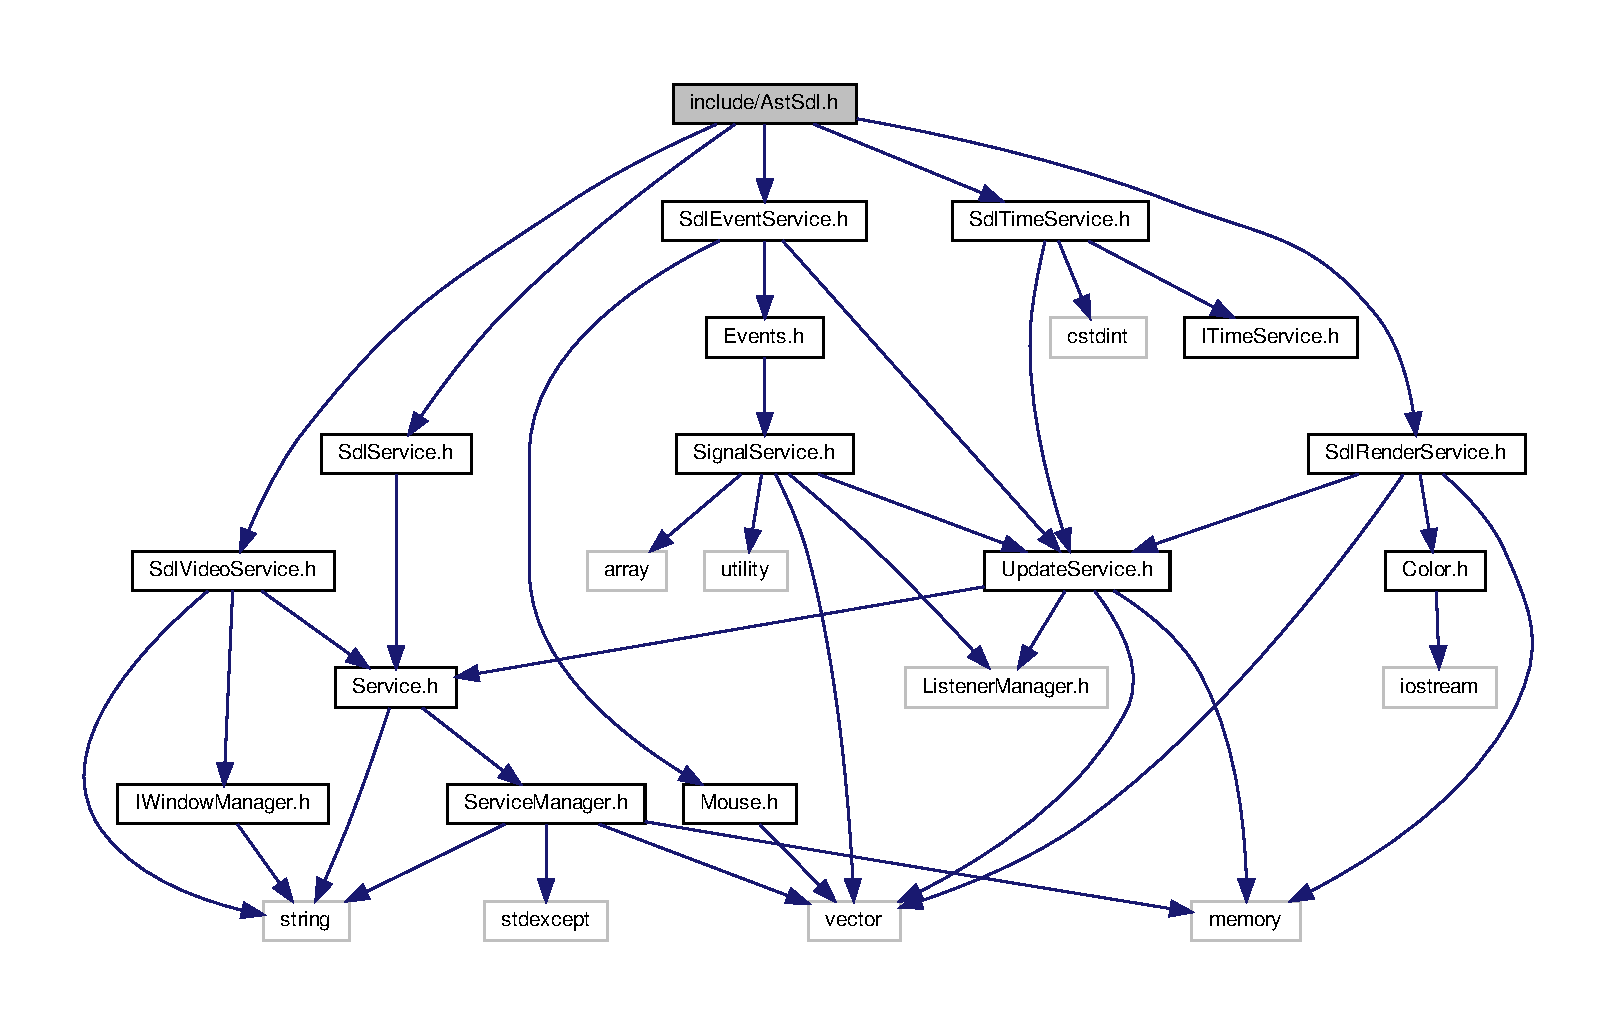
\includegraphics[width=350pt]{AstSdl_8h__incl}
\end{center}
\end{figure}


\subsection{Detailed Description}
This file defines public functions, templates and classes related to Simple Direct Layer S\+DL. 


\hypertarget{AstService_8h}{}\section{include/\+Ast\+Service.h File Reference}
\label{AstService_8h}\index{include/\+Ast\+Service.\+h@{include/\+Ast\+Service.\+h}}


This file defines public functions, templates and classes offered by the service module of A\+ST utilities.  


{\ttfamily \#include \char`\"{}Service.\+h\char`\"{}}\newline
{\ttfamily \#include \char`\"{}Update\+Service.\+h\char`\"{}}\newline
{\ttfamily \#include \char`\"{}State\+Service.\+h\char`\"{}}\newline
{\ttfamily \#include \char`\"{}Signal\+Service.\+h\char`\"{}}\newline
{\ttfamily \#include \char`\"{}Service\+Manager.\+h\char`\"{}}\newline
{\ttfamily \#include \char`\"{}I\+Time\+Service.\+h\char`\"{}}\newline
{\ttfamily \#include \char`\"{}I\+Window\+Manager.\+h\char`\"{}}\newline
Include dependency graph for Ast\+Service.\+h\+:\nopagebreak
\begin{figure}[H]
\begin{center}
\leavevmode
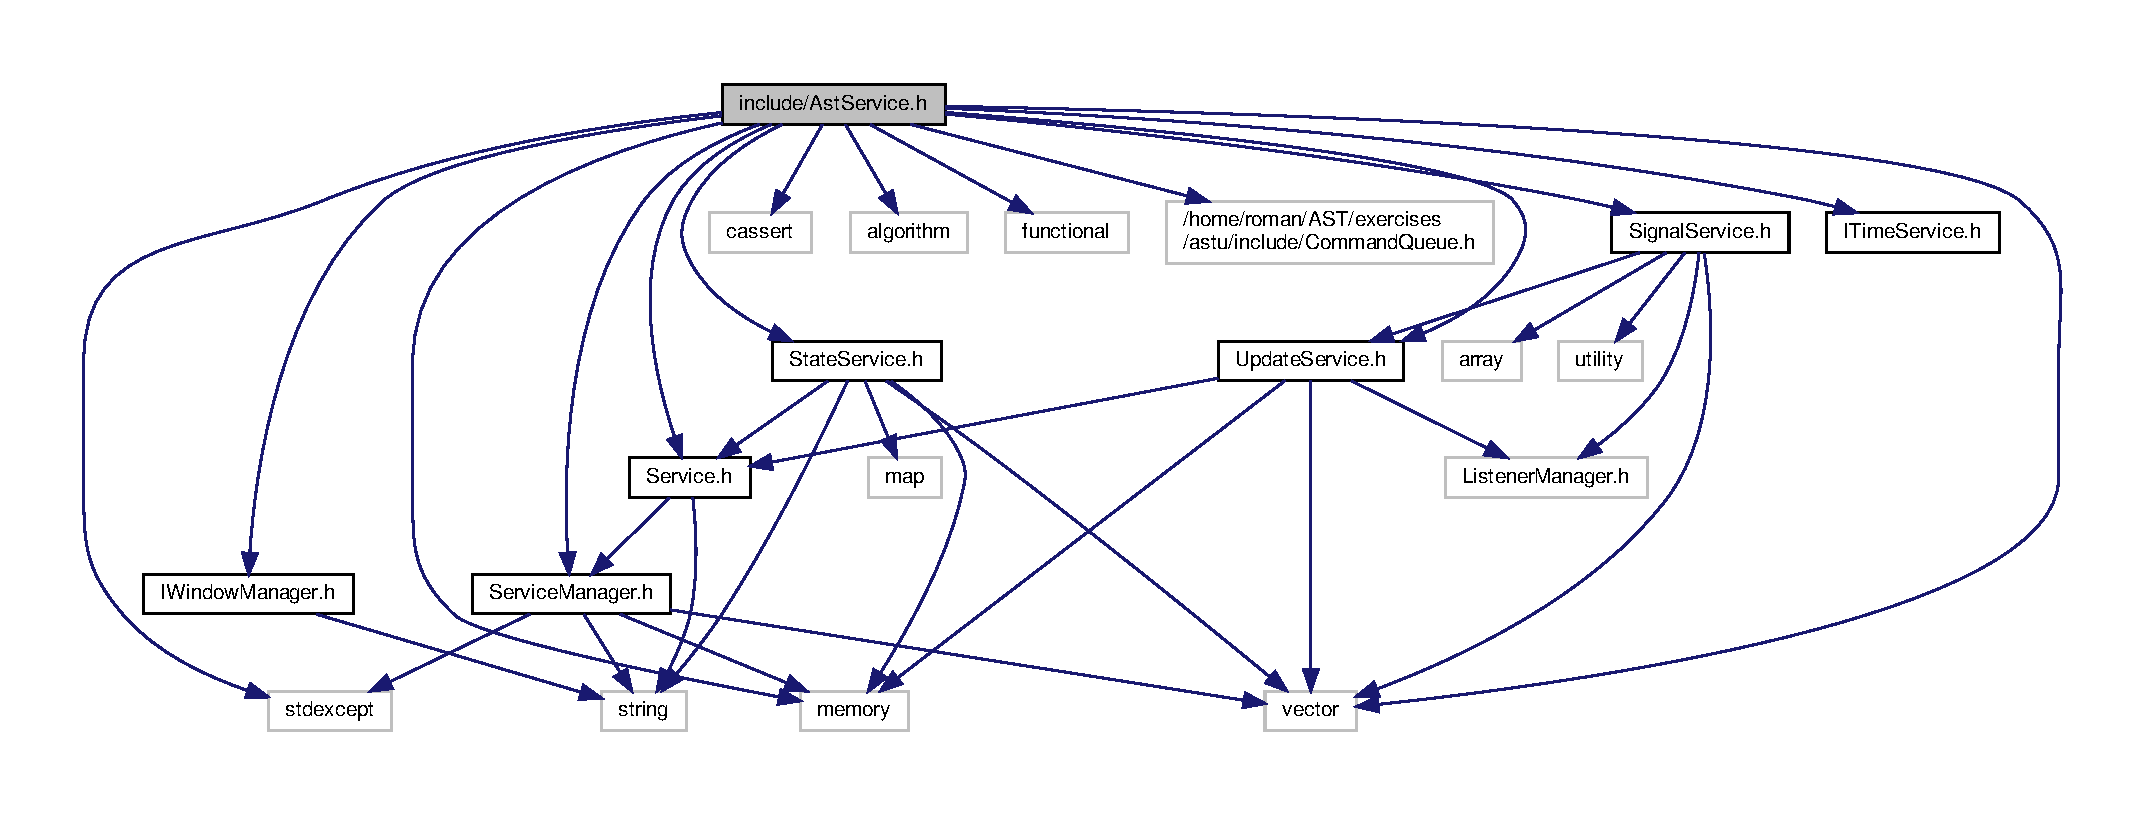
\includegraphics[width=350pt]{AstService_8h__incl}
\end{center}
\end{figure}


\subsection{Detailed Description}
This file defines public functions, templates and classes offered by the service module of A\+ST utilities. 


%--- End generated contents ---

% Index
\backmatter
\newpage
\phantomsection
\clearemptydoublepage
\addcontentsline{toc}{chapter}{Index}
\printindex

\end{document}
